% =============================================================================
% main_thesis.tex — Master Document (KOMA-Script scrreprt, A4, XeTeX/Tectonic)
% =============================================================================
\documentclass[
  11pt,
  a4paper,
  oneside,
  bibliography=totoc,
  listof=totoc,
  numbers=noenddot
]{scrreprt}

% --- Page Geometry (16.0 cm text width cleanly accommodates nomenclature tables) ---
\usepackage[
  a4paper,
  left=2.5cm,
  right=2.5cm,
  top=2.5cm,
  bottom=2.5cm,
  headheight=18pt
]{geometry}

% --- Fonts, Microtypography & Line Spacing ---
\usepackage{fontspec}
\usepackage{lmodern}
\usepackage{microtype}
\usepackage{setspace}
\setstretch{1.25}

% --- Mathematics, Tables & SI Units ---
\usepackage{amsmath,amssymb,mathtools}
\usepackage{booktabs,longtable,array,tabularx,multirow}
\usepackage{siunitx}
\DeclareSIUnit{\bpm}{bpm}
\sisetup{
  detect-all=true,
  per-mode=symbol,
  range-phrase=\text{--},
  range-units=single
}

% --- Graphics, Colors & Pure-TikZ Diagrams ---
\usepackage{graphicx}
\graphicspath{{../paper_orchestra_bundle/raw_materials/figures/}}
\usepackage[table]{xcolor}
\usepackage{tikz}
\usetikzlibrary{arrows.meta,positioning,shapes.geometric,fit,backgrounds,calc}

% Okabe-Ito Colorblind-Safe Palette (matched across Matplotlib & TikZ figures)
\definecolor{oiBlue}{HTML}{0072B2}
\definecolor{oiVermilion}{HTML}{D55E00}
\definecolor{oiGreen}{HTML}{009E73}
\definecolor{oiOrange}{HTML}{E69F00}
\definecolor{oiSky}{HTML}{56B4E9}
\definecolor{oiPurple}{HTML}{CC79A7}
\definecolor{oiGray}{HTML}{595959}
\definecolor{oiLightBg}{HTML}{F7F9FB}
\definecolor{oiWarnBg}{HTML}{FFF5F0}
\definecolor{oiSafeBg}{HTML}{F0F9F6}

% --- Headers, Captions & Floats ---
\usepackage[automark,headsepline]{scrlayer-scrpage}
\clearpairofpagestyles
\ihead{\headmark}
\ohead{\pagemark}
\pagestyle{scrheadings}

\usepackage{enumitem}
\setlist{nosep,topsep=4pt}

% --- Citations (bib entries verified 71/71 in seed_references.bib) ---
\usepackage[numbers,sort&compress]{natbib}

% --- Centralized Metadata & Locked Notation Contract ---
% =============================================================================
% Centralized Thesis Metadata (BTU Cottbus-Senftenberg, Faculty 1, Module 13600)
% Update bracketed placeholders prior to final university submission.
% =============================================================================

\newcommand{\ThesisTitle}{Physics-Constrained Machine Learning for Contactless Neonatal Radar Respiratory Monitoring: Parsimony, Causal Inductive Bias, and Safety-Aware Uncertainty Quantification}
\newcommand{\ThesisShortTitle}{Contactless NICU Radar Monitoring: Parsimony \& Safety-Aware UQ}
\newcommand{\ThesisType}{Master's Thesis}
\newcommand{\ThesisDegree}{Master of Science (M.Sc.) in Artificial Intelligence}
\newcommand{\ThesisModule}{Module 13600 (30\,ECTS)}

\newcommand{\ThesisAuthor}{Hosam Shibly}
\newcommand{\ThesisMatriculation}{[Insert Matriculation No.]}
\newcommand{\ThesisEmail}{[Insert BTU E-Mail Address]}

\newcommand{\ThesisUniversity}{Brandenburg University of Technology Cottbus-Senftenberg}
\newcommand{\ThesisFaculty}{Faculty 1: Mathematics, Computer Science, Physics, Electrical Engineering and Information Technology}
\newcommand{\ThesisChair}{[Insert Chair / Research Group Name]}

\newcommand{\FirstExaminer}{[Insert 1st Examiner, Title \& Name]}
\newcommand{\SecondExaminer}{[Insert 2nd Examiner, Title \& Name]}
\newcommand{\SubmissionPlace}{Cottbus, Germany}
\newcommand{\SubmissionDate}{[Insert Submission Date, e.g., DD Month YYYY]}

% Provenance & Freeze Identifiers (Read-Only Anchor)
\newcommand{\FrozenGitCommit}{\texttt{5e458c1}}
\newcommand{\FrozenArchiveHash}{\texttt{af33a83e157f7d2e}}
\newcommand{\FrozenArchiveHashFull}{\texttt{af33a83e157f7d2efb0f47e50c9544ee19bacb7da88ab0e0235ccead029cbcc4}}


\def\NOTATIONMACROSONLY{1}
% =============================================================================
% notation_glossary.tex
% Single Authoritative Symbol, Macro, Python Identifier & Figure-Label Lock
% Project : Non-Contact NICU Radar Breathing Monitoring (Master's Thesis)
% Authors : Frozen across Python docstrings (paper_workspace/src/*.py),
%           PaperOrchestra (google-research/paper-orchestra) dense inputs,
%           Matplotlib/TikZ figures, and LaTeX thesis chapters.
%
% USAGE:
%   1. In thesis main.tex PREAMBLE (loads macros only):
%        \def\NOTATIONMACROSONLY{1}
%        % =============================================================================
% notation_glossary.tex
% Single Authoritative Symbol, Macro, Python Identifier & Figure-Label Lock
% Project : Non-Contact NICU Radar Breathing Monitoring (Master's Thesis)
% Authors : Frozen across Python docstrings (paper_workspace/src/*.py),
%           PaperOrchestra (google-research/paper-orchestra) dense inputs,
%           Matplotlib/TikZ figures, and LaTeX thesis chapters.
%
% USAGE:
%   1. In thesis main.tex PREAMBLE (loads macros only):
%        \def\NOTATIONMACROSONLY{1}
%        % =============================================================================
% notation_glossary.tex
% Single Authoritative Symbol, Macro, Python Identifier & Figure-Label Lock
% Project : Non-Contact NICU Radar Breathing Monitoring (Master's Thesis)
% Authors : Frozen across Python docstrings (paper_workspace/src/*.py),
%           PaperOrchestra (google-research/paper-orchestra) dense inputs,
%           Matplotlib/TikZ figures, and LaTeX thesis chapters.
%
% USAGE:
%   1. In thesis main.tex PREAMBLE (loads macros only):
%        \def\NOTATIONMACROSONLY{1}
%        \input{paper_orchestra_bundle/raw_materials/notation_glossary.tex}
%   2. In thesis Appendix / Nomenclature chapter BODY (prints full tables):
%        \let\NOTATIONMACROSONLY\undefined
%        \input{paper_orchestra_bundle/raw_materials/notation_glossary.tex}
%   3. Requires standard LaTeX packages in parent document:
%        amsmath, amssymb, booktabs, longtable, array
% =============================================================================

% -----------------------------------------------------------------------------
% PART A: CANONICAL SEMANTIC LATEX MACROS (\providecommand avoids collisions)
% -----------------------------------------------------------------------------

% --- Physical & Radar Front-End Parameters (WP1) ---
\providecommand{\speedLight}{c}
\providecommand{\carrierFreq}{f_c}
\providecommand{\radarLambda}{\lambda}
\providecommand{\fsRadar}{f_s}
\providecommand{\fsRefRaw}{f_{s,\mathrm{ref}}}
\providecommand{\fsRefRate}{f_{s,\mathrm{rate}}}
\providecommand{\nomRange}{d_0}
\providecommand{\chestDisp}{d(t)}
\providecommand{\chestDispResp}{d_{\mathrm{resp}}(t)}
\providecommand{\chestDispCard}{d_{\mathrm{card}}(t)}
\providecommand{\chestDispRBM}{d_{\mathrm{RBM}}(t)}
\providecommand{\chestDispEst}{\hat{d}(t)}
\providecommand{\phaseSig}{\phi(t)}
\providecommand{\phaseZero}{\theta_0}
\providecommand{\modIndex}{\beta_{\mathrm{mod}}}
\providecommand{\besselJ}[2]{J_{#1}\!\left(#2\right)}
\providecommand{\iqI}{b_I(t)}
\providecommand{\iqQ}{b_Q(t)}
\providecommand{\iqComplex}{z(t)}
\providecommand{\iqGainImb}{g}
\providecommand{\iqPhaseSkew}{\psi}
\providecommand{\iqDcI}{c_I}
\providecommand{\iqDcQ}{c_Q}
\providecommand{\csdSignal}{x(t)}
\providecommand{\csdClean}{\hat{x}(t)}
\providecommand{\adPhase}{\hat{\phi}_{\mathrm{AD}}(t)}
\providecommand{\dacmPhase}{\hat{\phi}_{\mathrm{DACM}}(t)}

% --- Filtering, Windowing & STFT Decomposition (WP2) ---
\providecommand{\winSec}{W}
\providecommand{\updateSec}{\Delta_{\mathrm{upd}}}
\providecommand{\winSamples}{N_w}
\providecommand{\bandLow}{f_{\mathrm{low}}}
\providecommand{\bandHigh}{f_{\mathrm{high}}}
\providecommand{\firTaps}{M_{\mathrm{FIR}}}
\providecommand{\kaiserBeta}{\beta_{\mathrm{K}}}
\providecommand{\stftWin}{N_{\mathrm{win}}}
\providecommand{\stftHop}{H_{\mathrm{stft}}}
\providecommand{\stftNfft}{N_{\mathrm{FFT}}}
\providecommand{\stftComplex}{X[k,m]}
\providecommand{\stftMag}{\lvert X[k,m] \rvert}
\providecommand{\stftPhase}{\angle X[k,m]}
\providecommand{\stftMagFilt}{\lvert \hat{X}[k,m] \rvert}

% --- NMF/RBM Baseline vs HPSS Variants (WP2) ---
\providecommand{\nmfRank}{K_{\mathrm{NMF}}}
\providecommand{\nmfW}{\mathbf{W}}
\providecommand{\nmfH}{\mathbf{H}}
\providecommand{\hoyerSpar}{\sigma_{\mathrm{Hoyer}}}
\providecommand{\rbmAlpha}{\alpha_{\mathrm{RBM}}}
\providecommand{\rbmSparThresh}{\tau_{\mathrm{Hoyer}}}
\providecommand{\nRemoved}{n_{\mathrm{rem}}}
\providecommand{\hpssHarm}{S_H}
\providecommand{\hpssPerc}{S_P}
\providecommand{\hpssMask}{M_H}
\providecommand{\hpssMaskBand}{M_{H,\mathrm{band}}}
\providecommand{\hpssLenH}{L_H}
\providecommand{\hpssLenP}{L_P}
\providecommand{\hpssGamma}{\gamma}
\providecommand{\hpssEps}{\varepsilon}
\providecommand{\hpssMargin}{\beta_{\mathrm{sep}}}
\providecommand{\hpssKeptFrac}{\kappa_{\mathrm{kept}}}

% --- Harmonic NLS, HQI & Viterbi State-Space Tracking (WP3) ---
\providecommand{\psdFolded}{P(f)}
\providecommand{\autocorrFn}{r_{\mathrm{ac}}[\tau]}
\providecommand{\freqCoarse}{\hat{f}_{\mathrm{coarse}}}
\providecommand{\nlsOrder}{L_k}
\providecommand{\nlsRadius}{\Delta_{\mathrm{NLS}}}
\providecommand{\nlsStep}{\delta_{\mathrm{NLS}}}
\providecommand{\nlsCost}{\mathcal{J}_{\mathrm{NLS}}(f)}
\providecommand{\brEst}{\hat{f}_b}
\providecommand{\brRef}{f^{\mathrm{ref}}}
\providecommand{\hqiScore}{\mathrm{HQI}(f)}
\providecommand{\viterbiState}{q}
\providecommand{\viterbiEmit}{p_{\mathrm{emit}}}
\providecommand{\viterbiTrans}{A_{q',q}}
\providecommand{\brVit}{\hat{f}_b^{\mathrm{Vit}}}

% --- Synchronization, SQI & Selective Prediction (WP4) ---
\providecommand{\syncLag}{\hat{\tau}_s}
\providecommand{\satThresh}{\tau_{\mathrm{sat}}}
\providecommand{\validMask}{v_{s,w}}
\providecommand{\sqiScore}{\mathrm{SQI}_{s,w}}
\providecommand{\covLevel}{c_{\mathrm{cov}}}
\providecommand{\selRisk}{R(\covLevel)}
\providecommand{\aurcMetric}{\mathrm{AURC}}
\providecommand{\eaurcMetric}{\mathrm{E\text{-}AURC}}

% --- Cohort Evaluation, Clustered Agreement & Statistics (WP5) ---
\providecommand{\sessCount}{S}
\providecommand{\winSetSess}{\mathcal{W}_s}
\providecommand{\winErr}{e_{s,w}}
\providecommand{\rmseSession}[1]{\mathrm{RMSE}_{#1}}
\providecommand{\rmseSess}{\mathrm{RMSE}_{\mathrm{sess}}}
\providecommand{\rmsePool}{\mathrm{RMSE}_{\mathrm{pool}}}
\providecommand{\maeSess}{\mathrm{MAE}_{\mathrm{sess}}}
\providecommand{\accTau}[1]{\mathrm{Acc}@#1}
\providecommand{\rWithin}{r_{\mathrm{within}}}
\providecommand{\rWithinSessMean}{\bar{r}_{\mathrm{within}}^{(\mathrm{sess})}}
\providecommand{\baBias}{\hat{\mu}_d}
\providecommand{\baLoaLo}{\mathrm{LoA}_{\mathrm{lo}}}
\providecommand{\baLoaUp}{\mathrm{LoA}_{\mathrm{up}}}
\providecommand{\pairedDelta}{\Delta_s}
\providecommand{\tostMargin}{\Delta_{\mathrm{TOST}}}
\providecommand{\constGlobal}{\mathrm{const}_{\mathrm{global}}}
\providecommand{\constLoso}{\mathrm{const}_{\mathrm{LOSO}}}
\providecommand{\oracleSd}{\overline{\mathrm{SD}}_{\mathrm{ref}}}


% -----------------------------------------------------------------------------
% PART B: PRINTABLE NOMENCLATURE TABLES (suppressed if \NOTATIONMACROSONLY set)
% -----------------------------------------------------------------------------
\ifdefined\NOTATIONMACROSONLY\else

\section*{Master Notation Glossary and Code-to-Manuscript Contract}
\label{sec:notation_glossary}

{\sloppy
This glossary freezes every mathematical symbol, LaTeX macro, Python identifier
(\texttt{paper\_workspace/src/*.py}), and figure/plot axis label across the thesis
and all \texttt{PaperOrchestra} generation passes. Symbols marked \textbf{[LOCKED-v1]}
correspond to frozen provenance constants in \texttt{paper\_workspace/src/config.py}
(\texttt{SHA-256} manifest across all $15$ core modules, \texttt{pipeline\_version = main-v3-audit-fix-2});
symbols marked \textbf{[THESIS-NEW]} are introduced in work packages \texttt{WP1}--\texttt{WP5}
(denoted \texttt{[WPx TODO]} where code is not yet implemented in \texttt{paper\_workspace/src/}).
\par}

\begingroup
\footnotesize
\setlength{\tabcolsep}{3.5pt}
\begin{longtable}{@{}>{\raggedright\arraybackslash}p{0.13\textwidth} >{\raggedright\arraybackslash}p{0.19\textwidth} >{\raggedright\arraybackslash}p{0.28\textwidth} >{\raggedright\arraybackslash}p{0.20\textwidth} >{\raggedright\arraybackslash}p{0.12\textwidth}@{}}
\caption{Master Notation Contract: Physics, Demodulation, HPSS, Tracking, SQI, and Agreement Statistics.} \label{tab:master_notation} \\
\toprule
\textbf{Symbol} & \textbf{LaTeX Macro} & \textbf{Mathematical Definition \& Units} & \textbf{Python Identifier(s) \& Module} & \textbf{Figure / Prompt Label} \\
\midrule
\endfirsthead
\toprule
\textbf{Symbol} & \textbf{LaTeX Macro} & \textbf{Mathematical Definition \& Units} & \textbf{Python Identifier(s) \& Module} & \textbf{Figure / Prompt Label} \\
\midrule
\endhead
\midrule
\multicolumn{5}{r}{\textit{Continued on next page}} \\
\endfoot
\bottomrule
\endlastfoot

% --- 1. Physical Signal & CW I/Q Model ---
\multicolumn{5}{l}{\textbf{1. Radar Physics, I/Q Baseband \& Jacobi--Anger Phase Model (WP1)}} \\
$\carrierFreq, \speedLight$ & \texttt{\textbackslash carrierFreq}, \texttt{\textbackslash speedLight} & CW carrier frequency ($24\,\mathrm{GHz}$) and speed of light ($3\times 10^8\,\mathrm{m/s}$) \textbf{[LOCKED-v1]} & \texttt{FC\_HZ = 24e9} (\texttt{config.py}) & $f_c$ (GHz), $c$ \\
$\radarLambda$ & \texttt{\textbackslash radarLambda} & RF carrier wavelength $\lambda = c/f_c = 0.0125\,\mathrm{m}$ ($12.5\,\mathrm{mm}$ in \texttt{config.py}) \textbf{[LOCKED-v1]} & \texttt{LAMBDA\_M}, \texttt{LAMBDA\_MM}, \texttt{lam} (\texttt{config.py}, \texttt{demod.py}) & $\lambda$ (mm) \\
$\fsRadar$ & \texttt{\textbackslash fsRadar} & Decimated slow-time radar sampling rate ($16\,\mathrm{Hz}$) \textbf{[LOCKED-v1]} & \texttt{FS\_RADAR = 16} (\texttt{config.py}) & $f_s$ (Hz) \\
$\fsRefRaw, \fsRefRate$ & \texttt{\textbackslash fsRefRaw}, \texttt{\textbackslash fsRefRate} & Reference EDF raw respiration waveform ($256\,\mathrm{Hz}$) and rate ($1\,\mathrm{Hz}$, $1\,\mathrm{bpm}$ res.) \textbf{[LOCKED-v1]} & \texttt{FS\_REF\_RAW = 256}, \texttt{FS\_REF\_RATE = 1} (\texttt{config.py}) & $f_{s,\mathrm{ref}}, f_{s,\mathrm{rate}}$ \\
$\nomRange$ & \texttt{\textbackslash nomRange} & Static nominal antenna-to-chest standoff distance ($\mathrm{m}$) \textbf{[THESIS-NEW]} & \texttt{d\_0} (\texttt{WP1 TODO}) & $d_0$ (m) \\
$\chestDisp$ & \texttt{\textbackslash chestDisp} & Net physiological chest-wall displacement ($\mathrm{m}$ or $\mathrm{mm}$) \textbf{[THESIS-NEW]} & \texttt{d\_true} (\texttt{WP1 TODO}; dist.\ from \texttt{d\_hat}) & $d(t)$ (mm) \\
$\chestDispResp$, $\chestDispCard$, $\chestDispRBM$ & \texttt{\textbackslash chestDisp\allowbreak Resp}, \texttt{\textbackslash chestDisp\allowbreak Card}, \texttt{\textbackslash chestDisp\allowbreak RBM} & Respiratory, cardiogenic, and random-body-movement components summing to $\chestDisp$ \textbf{[THESIS-NEW]} & \texttt{WP1 TODO} synth simulator & $d_{\mathrm{resp}}$, $d_{\mathrm{card}}$, $d_{\mathrm{RBM}}$ \\
$\phaseSig, \phaseZero$ & \texttt{\textbackslash phaseSig}, \texttt{\textbackslash phaseZero} & Total RF phase $\phaseSig = \phaseZero + \frac{4\pi}{\radarLambda}\chestDisp$ ($\mathrm{rad}$) and equilibrium carrier phase $\phaseZero = \frac{4\pi\nomRange}{\radarLambda}+\phi_{\mathrm{rf}} \pmod{2\pi}$ \textbf{[THESIS-NEW]} & \texttt{theta\_0} (\texttt{WP1 TODO} Jacobi--Anger / IQ calib) & $\phi(t), \theta_0$ (rad) \\
$\iqI$, $\iqQ$, $\iqComplex$ & \texttt{\textbackslash iqI}, \texttt{\textbackslash iqQ}, \texttt{\textbackslash iqComplex} & ADC baseband channels ($\mathrm{V}$) and raw complex baseband $\iqComplex = \iqI + j\iqQ$ \textbf{[LOCKED-v1]} & \texttt{bI}, \texttt{bQ} (\texttt{demod.py}, \texttt{data\_\allowbreak loader.py}) & $b_I(t)$, $b_Q(t)$, $z(t)$ \\
$\iqDcI, \iqDcQ, \iqGainImb, \iqPhaseSkew$ & \texttt{\textbackslash iqDcI}, \texttt{\textbackslash iqDcQ}, \texttt{\textbackslash iqGainImb}, \texttt{\textbackslash iqPhaseSkew} & Receiver I/Q DC offsets, gain ratio $A_Q/A_I$, and quadrature skew error ($\mathrm{rad}$) \textbf{[THESIS-NEW]} & \texttt{dc\_i, dc\_q, iq\_gain, iq\_skew} (\texttt{WP1 TODO}) & $(c_I, c_Q, g, \psi)$ \\
$\csdSignal$ & \texttt{\textbackslash csdSignal} & Per-window mean-centered complex baseband $\csdSignal = (b_I - \bar{b}_I) + j(b_Q - \bar{b}_Q)$ via \texttt{csd()} \textbf{[LOCKED-v1]} & \texttt{x} (\texttt{demod.csd}, \texttt{run\_\allowbreak measurement.py}) & $x(t)$ (complex) \\
$\adPhase$, $\dacmPhase$ & \texttt{\textbackslash adPhase}, \texttt{\textbackslash dacmPhase} & Unwrapped arctangent $\frac{\lambda}{4\pi}\mathrm{unwrap}(\mathrm{atan2}(\Delta b_Q,\Delta b_I))$ (\texttt{demod.ad}: unused in active scoring, audit A10) vs DACM phase \textbf{[v1 / WP1]} & \texttt{ad} (\texttt{demod.py}, unused); \texttt{phase\_\allowbreak dacm} (\texttt{WP1 TODO}) & $\hat{\phi}_{\mathrm{AD}}$, $\hat{\phi}_{\mathrm{DACM}}$ \\
$\besselJ{n}{\modIndex}$ & \texttt{\textbackslash besselJ\{n\}\allowbreak\{\textbackslash modIndex\}} & $n$-th Bessel function of first kind at modulation depth $\modIndex = 4\pi A_r / \lambda$ \textbf{[THESIS-NEW]} & \texttt{scipy.\allowbreak special.jv} (\texttt{WP1 TODO} analyzer) & $J_n(\beta_{\mathrm{mod}})$ \\
$\chestDispEst$ & \texttt{\textbackslash chestDispEst} & Bandpass-filtered complex signal from \texttt{bandpass()}: upstream \texttt{d\_raw}, Branch-A \texttt{d\_hat}, Branch-B \texttt{d\_hpss} \textbf{[LOCKED-v1]} & \texttt{d\_raw, d\_hat, d\_hpss} (\texttt{filtering.py}, \texttt{run\_measurement.py}) & $\hat{d}(t)$ (a.u.) \\

% --- 2. Windowing, STFT & HPSS ---
\multicolumn{5}{l}{\textbf{2. Windowing, STFT Representation, NMF Baseline \& HPSS Variants (WP2)}} \\
$\winSec$, $\updateSec$, $\winSamples$ & \texttt{\textbackslash winSec}, \texttt{\textbackslash updateSec}, \texttt{\textbackslash winSamples} & Sliding analysis window $30\,\mathrm{s}$, hop $2\,\mathrm{s}$ ($28\,\mathrm{s}$ overlap), samples $\winSamples = 480$ \textbf{[LOCKED-v1]} & \texttt{WIN\_S, OVERLAP\_S, UPDATE\_S, WIN\_\allowbreak SAMPLES} (\texttt{config.py}) & $W=30\,\mathrm{s}$ \\
$\bandLow$, $\bandHigh$, $\firTaps$, $\kaiserBeta$ & \texttt{\textbackslash bandLow}, \texttt{\textbackslash bandHigh}, \texttt{\textbackslash firTaps}, \texttt{\textbackslash kaiserBeta} & Zero-phase Kaiser FIR passband $[0.3, 3.0]\,\mathrm{Hz}$ ($18$--$180\,\mathrm{bpm}$), $64$ taps, $\beta_{\mathrm{K}}=6.5$ \textbf{[LOCKED-v1]} & \texttt{BAND\_\allowbreak LOW\_\allowbreak HZ, BAND\_\allowbreak HIGH\_\allowbreak HZ, FIR\_\allowbreak TAPS, KAISER\_\allowbreak BETA} & $[0.3, 3.0]\,\mathrm{Hz}$ \\
$\stftWin$, $\stftHop$, $\stftNfft$ & \texttt{\textbackslash stftWin}, \texttt{\textbackslash stftHop}, \texttt{\textbackslash stftNfft} & STFT \emph{rectangular} window $48$ ($3\,\mathrm{s}$), hop $16$ ($1\,\mathrm{s}$), FFT size $256$ ($\Delta f=3.75\,\mathrm{bpm}$) \textbf{[LOCKED-v1]} & \texttt{STFT\_\allowbreak WIN, STFT\_\allowbreak HOP, STFT\_\allowbreak NFFT} (\texttt{config.py}, \texttt{rbm\_\allowbreak nmf.py}) & $48/16/256$ rect.\ STFT \\
$\stftComplex$, $\stftMag$, $\stftPhase$, $\stftMagFilt$ & \texttt{\textbackslash stftComplex}, \texttt{\textbackslash stftMag}, \texttt{\textbackslash stftPhase}, \texttt{\textbackslash stftMag\allowbreak Filt} & Two-sided complex STFT ($256 \times T_f$), magnitude, wrapped phase, and post-\texttt{env\_\allowbreak normalize} magnitude ($\times\mathrm{clip}(\mathrm{med}(M_{\mathrm{frame}})/M_{\mathrm{frame}},$ $0.5, 2.0)$) \textbf{[LOCKED-v1]} & \texttt{X, mag, phase, mag\_\allowbreak filt} (\texttt{rbm\_\allowbreak nmf.py}, \texttt{hpss.py}) & $|X[k,m]|$, $|\hat{X}[k,m]|$ \\
$\hpssLenH, \hpssLenP$ & \texttt{\textbackslash hpssLenH}, \texttt{\textbackslash hpssLenP} & Horizontal (time) and vertical (frequency) median kernel lengths ($7$ frames, $21$ bins) \textbf{[LOCKED-v1]} & \texttt{L\_HARM = 7}, \texttt{L\_PERC = 21} (\texttt{hpss.py}) & $(L_H, L_P)$ \\
$\hpssHarm$ & \texttt{\textbackslash hpssHarm} & Harmonic spectrogram estimate via time-axis median filter $\mathrm{med}_{m}(|X[k,m]|; \hpssLenH)$ \textbf{[LOCKED-v1]} & \texttt{s\_harm} (\texttt{hpss.hpss\_filter}) & $S_H[k,m]$ \\
$\hpssPerc$ & \texttt{\textbackslash hpssPerc} & Percussive/motion spectrogram estimate via freq-axis median filter $\mathrm{med}_{k}(|X[k,m]|; \hpssLenP)$ \textbf{[LOCKED-v1]} & \texttt{s\_perc} (\texttt{hpss.hpss\_filter}) & $S_P[k,m]$ \\
$\hpssGamma, \hpssEps, \hpssMargin$ & \texttt{\textbackslash hpssGamma}, \texttt{\textbackslash hpssEps}, \texttt{\textbackslash hpssMargin} & Wiener power exponent ($\gamma=2.0$), stabilizer ($\varepsilon=10^{-12}$) \textbf{[LOCKED-v1]}; Driedger separation factor $\beta_{\mathrm{sep}}$ \textbf{[THESIS-NEW]} & \texttt{GAMMA = 2.0}, \texttt{EPS = 1e-12} (\texttt{hpss.py}); \texttt{WP2 TODO} & $\gamma, \varepsilon, \beta_{\mathrm{sep}}$ \\
$\hpssMask$ & \texttt{\textbackslash hpssMask} & Harmonic soft Wiener mask $\hpssMask = \hpssHarm^\gamma / (\hpssHarm^\gamma + \hpssPerc^\gamma + \varepsilon) \in [0,1]$ on two-sided \texttt{fftshift} STFT \textbf{[LOCKED-v1]} & \texttt{mask, mask\_s} (\texttt{hpss.hpss\_filter}) & $M_H[k,m]$ \\
$\hpssMaskBand$ & \texttt{\textbackslash hpssMaskBand} & Proposed band-restricted or directional harmonic mask restricted to $|f_k| \in [\bandLow, \bandHigh]$ \textbf{[THESIS-NEW]} & \texttt{WP2 TODO} (dist.\ from \texttt{v1} \texttt{mask\_s}) & $M_{H,\mathrm{band}}$ \\
$\nmfRank, \nmfW, \nmfH$ & \texttt{\textbackslash nmfRank}, \texttt{\textbackslash nmfW}, \texttt{\textbackslash nmfH} & Baseline NMF rank ($K_{\mathrm{NMF}}=11$), basis dictionary $\nmfW \in \mathbb{R}_{\ge 0}^{F\times K}$, temporal activations $\nmfH \in \mathbb{R}_{\ge 0}^{K\times T_f}$ \textbf{[LOCKED-v1]} & \texttt{NMF\_K = 11}, \texttt{W}, \texttt{H} (\texttt{config.py}, \texttt{rbm\_nmf.py}) & $\mathbf{W}, \mathbf{H}$ \\
$\rbmAlpha$, $\hoyerSpar$, $\rbmSparThresh$, $\nRemoved$ & \texttt{\textbackslash rbmAlpha}, \texttt{\textbackslash hoyerSpar}, \texttt{\textbackslash rbmSpar\allowbreak Thresh}, \texttt{\textbackslash nRemoved} & \texttt{beltrao\_\allowbreak tuned} thresh $\alpha_{\mathrm{RBM}}=3.0$ (top-3 frac $>0.6$); \texttt{attached\_\allowbreak locked} row Hoyer sparsity $>\tau_{\mathrm{Hoyer}}=0.55$ ($\&\ \max h_k > 2\bar{H}$); removed NMF basis count $n_{\mathrm{rem}}$ ($>2\Rightarrow$ heavy move) \textbf{[LOCKED-v1]} & \texttt{RBM\_\allowbreak ALPHA}, \texttt{hoyer\_\allowbreak sparsity}, \texttt{s\_thresh=0.55}, \texttt{n\_removed} (\texttt{rbm\_\allowbreak nmf.py}) & $\sigma_{\mathrm{Hoyer}}$, $\tau_{\mathrm{Hoyer}}$, $n_{\mathrm{rem}}$ \\
$\csdClean$, $\hpssKeptFrac$ & \texttt{\textbackslash csdClean}, \texttt{\textbackslash hpssKept\allowbreak Frac} & ISTFT-reconstructed complex signal and pre-\texttt{env\_\allowbreak normalize} full-spectrum $L_1$ magnitude fraction $\sum|\hat{X}_{\mathrm{raw}}|/\sum|X|$ \textbf{[LOCKED-v1]} & \texttt{x\_hat}, \texttt{kept\_\allowbreak frac} (\texttt{hpss.\allowbreak mitigate\_\allowbreak hpss}) & $\hat{x}(t)$, $\kappa_{\mathrm{kept}}$ \\

% --- 3. Estimation, HQI & Viterbi ---
\multicolumn{5}{l}{\textbf{3. Spectral/NLS Estimation, HQI Disambiguation \& Viterbi Tracking (WP3)}} \\
$\psdFolded$, $\autocorrFn$, $\freqCoarse$ & \texttt{\textbackslash psdFolded}, \texttt{\textbackslash autocorrFn}, \texttt{\textbackslash freqCoarse} & Folded PSD ($|X(+f)|^2+|X(-f)|^2$), normalized autocorr of $\chestDispEst$, and coarse breathing peak ($\mathrm{Hz}$, prom.\ $\ge 0.10$) \textbf{[LOCKED-v1]} & \texttt{Pf}, \texttt{r}, \texttt{f\_coarse} (\texttt{estimation.py}, \texttt{filtering.py}) & $\hat{f}_{\mathrm{coarse}}$ (bpm) \\
$\nlsOrder$, $\nlsRadius$, $\nlsStep$, $\nlsCost$ & \texttt{\textbackslash nlsOrder}, \texttt{\textbackslash nlsRadius}, \texttt{\textbackslash nlsStep}, \texttt{\textbackslash nlsCost} & Harmonic NLS order ($L_k=2$), coarse radius ($\pm 5\,\mathrm{bpm}$), step ($0.1\,\mathrm{bpm}$), objective $\sum_{\ell=1}^{L_k} w_\ell P(\ell f)$ \textbf{[LOCKED-v1]} & \texttt{NLS\_\allowbreak LK = 2}, \texttt{NLS\_\allowbreak RADIUS\_\allowbreak BPM = 5.0}, \texttt{NLS\_\allowbreak GRID\_\allowbreak STEP\_\allowbreak BPM = 0.1}, \texttt{score} & $\mathcal{J}_{\mathrm{NLS}}(f)$, $L_k=2$ \\
$\brEst$ & \texttt{\textbackslash brEst} & Window-level breathing rate estimate ($\mathrm{bpm}$, $60\hat{f}_b$) from NMF/HPSS/NLS/DFT branch \textbf{[LOCKED-v1]} & \texttt{bestf} (\texttt{estimation.py}); \texttt{est, est\_\allowbreak hpss, est\_\allowbreak nls, est\_\allowbreak dft} (\texttt{cache}) & $\hat{f}_b$ (bpm) \\
$\hqiScore$ & \texttt{\textbackslash hqiScore} & Harmonic Quality Index disambiguating fundamental vs $0.5\times$/$2\times$ octave errors \textbf{[THESIS-NEW]} & \texttt{hqi} (\texttt{WP3 TODO} estimator) & $\mathrm{HQI}(f)$ \\
$\viterbiState$, $\viterbiEmit$, $\viterbiTrans$, $\brVit$ & \texttt{\textbackslash viterbiState}, \texttt{\textbackslash viterbiEmit}, \texttt{\textbackslash viterbiTrans}, \texttt{\textbackslash brVit} & HMM breathing-rate state grid, emission likelihood, transition matrix, and Viterbi path ($\mathrm{bpm}$) \textbf{[THESIS-NEW]} & \texttt{states\_\allowbreak bpm, log\_\allowbreak emit, log\_\allowbreak trans, est\_\allowbreak viterbi} (\texttt{WP3 TODO}) & $q$, $A_{q',q}$, $\hat{f}_b^{\mathrm{Vit}}$ \\

% --- 4. Sync, SQI & Selective Prediction ---
\multicolumn{5}{l}{\textbf{4. Reference Alignment, Signal Quality Indices \& Selective Prediction (WP4)}} \\
$\syncLag$ & \texttt{\textbackslash syncLag} & Metadata-anchored cross-correlation radar-vs-EDF alignment lag ($\pm 60\,\mathrm{s}$ search) \textbf{[LOCKED-v1]} & \texttt{lag}, \texttt{lag\_s} (\texttt{evaluation.\allowbreak sync\_\allowbreak arrays}, \texttt{cache}) & $\hat{\tau}_s$ (s) \\
$\satThresh$, $\validMask$, $\brRef$ & \texttt{\textbackslash satThresh}, \texttt{\textbackslash validMask}, \texttt{\textbackslash brRef} & ADC saturation cutoff ($2.99$, zero saturated seconds allowed), window validity boolean, and $30\,\mathrm{s}$ mean ref BR ($\mathrm{bpm}$) \textbf{[LOCKED-v1]} & \texttt{sat\_\allowbreak thresh=2.99}, \texttt{valid}, \texttt{vwin}, \texttt{ref} (\texttt{evaluation.py}) & $f^{\mathrm{ref}}_{s,w}$ (bpm) \\
$\sqiScore$ & \texttt{\textbackslash sqiScore} & Interpretable continuous Signal Quality Index for window $w$ in session $s$, $\sqiScore \in [0, 1]$ \textbf{[THESIS-NEW]} & \texttt{sqi} (\texttt{WP4 TODO} selective gating) & $\mathrm{SQI} \in [0, 1]$ \\
$\covLevel$, $\selRisk$, $\aurcMetric$, $\eaurcMetric$ & \texttt{\textbackslash covLevel}, \texttt{\textbackslash selRisk}, \texttt{\textbackslash aurcMetric}, \texttt{\textbackslash eaurcMetric} & Retention coverage, risk at coverage $c_{\mathrm{cov}}$ ($\mathrm{RMSE}^2$/$\mathrm{MAE}$), Area Under Risk--Coverage Curve, and Excess-AURC \textbf{[THESIS-NEW]} & \texttt{coverage, risk, aurc, e\_aurc} (\texttt{WP4 TODO}) & $\mathrm{AURC}$, $c_{\mathrm{cov}}$ \\

% --- 5. Statistical Evaluation ---
\multicolumn{5}{l}{\textbf{5. Cohort Performance, Agreement \& Hypothesis Testing Metrics (WP5)}} \\
$\sessCount$, $\winSetSess$, $\winErr$ & \texttt{\textbackslash sessCount}, \texttt{\textbackslash winSetSess}, \texttt{\textbackslash winErr} & Valid sessions in cohort, valid window index set $\winSetSess$, and signed error $\hat{f}_{b,s,w} - f^{\mathrm{ref}}_{s,w}$ ($\mathrm{bpm}$) & \texttt{len(sess)}, \texttt{v}, \texttt{err\_n / err\_h} (\texttt{final\_\allowbreak review.py}) & $e_{s,w}$ (bpm) \\
$\rmseSession{s}$ & \texttt{\textbackslash rmseSession\allowbreak \{s\}} & Within-session Root Mean Squared Error $\sqrt{\frac{1}{|\winSetSess|}\sum_{w\in\winSetSess} e_{s,w}^2}$ ($\mathrm{bpm}$) \textbf{[LOCKED-v1]} & \texttt{\_\allowbreak per\_\allowbreak session\_\allowbreak rmse(\allowbreak sess, key)} (\texttt{final\_\allowbreak review.py}) & $\mathrm{RMSE}_s$ (bpm) \\
$\rmseSess$, $\maeSess$ & \texttt{\textbackslash rmseSess}, \texttt{\textbackslash maeSess} & Equal-session macro-averages $\frac{1}{S}\sum_{s=1}^S \rmseSession{s}$ and $\mathrm{MAE}_{\mathrm{sess}}$ ($\mathrm{bpm}$; \texttt{final\_\allowbreak review.py} also reports session median) \textbf{[LOCKED-v1]} & \texttt{baselines[c][b]}, \texttt{rmse\_\allowbreak *\_\allowbreak per\_\allowbreak window}, \texttt{mae\_\allowbreak *\_\allowbreak session\_\allowbreak median} & $\mathrm{RMSE}_{\mathrm{sess}}$, $\mathrm{MAE}_{\mathrm{sess}}$ \\
$\rmsePool$ & \texttt{\textbackslash rmsePool} & Window-pooled RMSE $\sqrt{\frac{1}{\sum_s|\winSetSess|}\sum_{s,w} e_{s,w}^2}$ ($\mathrm{bpm}$; dist.\ from $\rmseSess$) \textbf{[LOCKED-v1]} & \texttt{pooled\_\allowbreak rmse\_\allowbreak nmf\_\allowbreak hpss\_\allowbreak rawnls}, \texttt{scores()['rmse']} & $\mathrm{RMSE}_{\mathrm{pool}}$ (bpm) \\
$\rWithin$ & \texttt{\textbackslash rWithin} & Bland--Altman (1995) ANCOVA pooled within-session Pearson correlation removing session means \textbf{[THESIS-NEW]} & \texttt{r\_\allowbreak within\_\allowbreak rmcorr} (\texttt{WP5 TODO} repeated-measures stats) & $r_{\mathrm{within}}$ \\
$\rWithinSessMean$ & \texttt{\textbackslash rWithin\allowbreak SessMean} & Unweighted cohort mean of per-session Pearson $r_s$ computed in \texttt{final\_\allowbreak review.py} \textbf{[LOCKED-v1]} & \texttt{within\_\allowbreak session\_\allowbreak pearson\_\allowbreak r\_\allowbreak *\_\allowbreak mean} (\texttt{final\_\allowbreak review.py:\allowbreak 290-291}) & $\bar{r}_{\mathrm{within}}^{(\mathrm{sess})}$ \\
$\accTau{\delta}$ & \texttt{\textbackslash accTau\allowbreak \{\textbackslash delta\}} & Percentage of windows with $|\winErr| < \delta\,\mathrm{bpm}$ for $\delta \in \{3, 6, 10\}$ \textbf{[LOCKED-v1]} & \texttt{acc3, acc6, acc10} (\texttt{evaluation.\allowbreak scores:193}) & $\mathrm{Acc}@\delta$ (\%) \\
$\baBias$, $\baLoaLo$, $\baLoaUp$ & \texttt{\textbackslash baBias}, \texttt{\textbackslash baLoaLo}, \texttt{\textbackslash baLoaUp} & Mean error bias and $\pm 1.96\,\mathrm{SD}$ Limits of Agreement (clustered ANOVA for final thesis) & \texttt{bias, loa\_lo, loa\_up} (\texttt{evaluation.py}); \texttt{bland\_\allowbreak altman\_\allowbreak pooled\_\allowbreak *} & Bias $\pm 1.96\,\mathrm{SD}$ \\
$\pairedDelta$, $\tostMargin$ & \texttt{\textbackslash pairedDelta}, \texttt{\textbackslash tostMargin} & Paired delta $\rmseSession{\mathrm{new},s} - \rmseSession{\mathrm{base},s}$ and pre-registered TOST bound $0.50\,\mathrm{bpm}$ \textbf{[LOCKED-v1]} & \texttt{delta}, \texttt{TOST\_\allowbreak MARGIN = 0.50} (\texttt{final\_\allowbreak review.py}) & $\Delta_s$, $\Delta_{\mathrm{TOST}}$ \\
$\constGlobal$, $\constLoso$, $\oracleSd$ & \texttt{\textbackslash constGlobal}, \texttt{\textbackslash constLoso}, \texttt{\textbackslash oracleSd} & In-sample pooled mean baseline, zero-leakage LOSO median predictor, and within-session reference SD oracle & \texttt{const\_\allowbreak global\_\allowbreak oracle, const\_\allowbreak loso, session\_\allowbreak mean\_\allowbreak oracle} & $\constLoso$, $\overline{\mathrm{SD}}_{\mathrm{ref}}$ \\
\end{longtable}
\endgroup


\section*{Notation Disambiguation \& Anti-Drift Guardrails for PaperOrchestra}
\label{sec:notation_guardrails}

All \texttt{PaperOrchestra} drafting agents, dense-input outlines, and Python
docstrings MUST obey the five disambiguation rules in
Table~\ref{tab:notation_guardrails} to eliminate collisions observed in legacy logs
and preliminary scripts.

\begin{table}[htbp]
\centering
\footnotesize
\setlength{\tabcolsep}{4pt}
\caption{Critical Symbol \& Identifier Disambiguation Rules.} \label{tab:notation_guardrails}
\begin{tabular}{@{}>{\raggedright\arraybackslash}p{0.19\textwidth} >{\raggedright\arraybackslash}p{0.34\textwidth} >{\raggedright\arraybackslash}p{0.41\textwidth}@{}}
\toprule
\textbf{Confused Pair} & \textbf{Root Cause of Ambiguity} & \textbf{Mandatory Thesis \& Code Rule} \\
\midrule
$\chestDisp$ vs $\chestDispEst$ vs $\csdSignal$ &
In \texttt{run\_\allowbreak measurement.py}, \texttt{csd()} produces mean-centered complex $\csdSignal$; downstream calls pass \texttt{d\_raw = bandpass(x)} into \texttt{mitigate} / \texttt{mitigate\_\allowbreak hpss}, yielding \texttt{d\_hat} (NMF) and \texttt{d\_hpss} (HPSS)---none are metric displacement $\chestDisp$ ($\mathrm{mm}$) unless calibrated. &
Use $\chestDisp$ solely for physical chest displacement ($\mathrm{mm}$); $\csdSignal$ for mean-centered complex baseband; $\chestDispEst$ explicitly distinguished as \texttt{d\_raw}, \texttt{d\_hat}, or \texttt{d\_hpss}. Never equate $|\mathrm{bandpass}(\csdSignal)|$ with metric displacement in $\mathrm{mm}$. \\
\addlinespace
$\rmseSess$ vs \texttt{rmse\_\allowbreak *\_\allowbreak per\_\allowbreak window} vs $\rmsePool$ &
In \texttt{paper\_\allowbreak workspace/\allowbreak src/\allowbreak final\_\allowbreak review.py:\allowbreak 255}, the JSON field \texttt{rmse\_\allowbreak hpss\_\allowbreak per\_\allowbreak window} stores the \emph{unweighted session mean} of $\rmseSession{s}$, whereas \texttt{evaluation.\allowbreak scores()['rmse']} and \texttt{pooled\_\allowbreak rmse\_\allowbreak *} aggregate squared errors across windows. &
Report $\rmseSess$ (\texttt{\textbackslash rmseSess}) as the primary equal-session KPI ($6.798\,\mathrm{bpm}$ HPSS on \texttt{PAPER\_18}); explicitly label window-pooled values as $\rmsePool$ (\texttt{\textbackslash rmsePool}; $7.217\,\mathrm{bpm}$ on \texttt{PAPER\_18}). \\
\addlinespace
$\rWithin$ vs $\rWithinSessMean$ &
Bland \& Altman (1995) $\rWithin$ uses ANCOVA residual sums of squares weighted by $|\winSetSess|-1$ across sessions, whereas \texttt{final\_\allowbreak review.py:\allowbreak 290-291} averages per-session $r_s$ unweighted ($\bar{r}_{\mathrm{within}}^{(\mathrm{sess})} = 0.465$ HPSS on \texttt{PAPER\_18}). &
Reserve $\rWithin$ (\texttt{\textbackslash rWithin}) strictly for Bland--Altman ANCOVA \texttt{rmcorr}, and denote unweighted session averages as $\rWithinSessMean$ (\texttt{\textbackslash rWithin\allowbreak SessMean}). Never compute pooled cross-session Pearson $r$. \\
\addlinespace
$\hpssMask$ vs $\hpssMaskBand$ &
In \texttt{hpss.py:42}, locked \texttt{v1} computes $\hpssMask = \frac{\hpssHarm^\gamma}{\hpssHarm^\gamma + \hpssPerc^\gamma + \varepsilon}$ (single $\varepsilon$ in denominator only) across the full two-sided \texttt{fftshift} FFT ($F=256$); the Python variable \texttt{mask\_s} is simply the \texttt{fftshift}-centered mask, NOT a band-restricted mask. &
Write the exact denominator $\hpssHarm^\gamma + \hpssPerc^\gamma + \varepsilon$ when documenting locked \texttt{v1}, note the two-sided STFT domain (\texttt{hpss.py:20-23}), and reserve $\hpssMaskBand$ strictly for the proposed \texttt{WP2} in-band/directional mask ($|f_k| \in [\bandLow, \bandHigh]$). \\
\addlinespace
$\nmfH$ / $\hpssHarm$ notation collision &
Audio papers sometimes write $H$ for harmonic spectrogram while NMF writes $\nmfH$ for temporal activation matrices ($\mathbf{W}\mathbf{H}$). &
Use bold $\nmfW$, $\nmfH$ exclusively for NMF decomposition factors, and reserve $\hpssHarm$, $\hpssPerc$ (\texttt{\textbackslash hpssHarm}, \texttt{\textbackslash hpssPerc}) for median-filtered HPSS spectrograms. \\
\bottomrule
\end{tabular}
\end{table}

\fi

%   2. In thesis Appendix / Nomenclature chapter BODY (prints full tables):
%        \let\NOTATIONMACROSONLY\undefined
%        % =============================================================================
% notation_glossary.tex
% Single Authoritative Symbol, Macro, Python Identifier & Figure-Label Lock
% Project : Non-Contact NICU Radar Breathing Monitoring (Master's Thesis)
% Authors : Frozen across Python docstrings (paper_workspace/src/*.py),
%           PaperOrchestra (google-research/paper-orchestra) dense inputs,
%           Matplotlib/TikZ figures, and LaTeX thesis chapters.
%
% USAGE:
%   1. In thesis main.tex PREAMBLE (loads macros only):
%        \def\NOTATIONMACROSONLY{1}
%        \input{paper_orchestra_bundle/raw_materials/notation_glossary.tex}
%   2. In thesis Appendix / Nomenclature chapter BODY (prints full tables):
%        \let\NOTATIONMACROSONLY\undefined
%        \input{paper_orchestra_bundle/raw_materials/notation_glossary.tex}
%   3. Requires standard LaTeX packages in parent document:
%        amsmath, amssymb, booktabs, longtable, array
% =============================================================================

% -----------------------------------------------------------------------------
% PART A: CANONICAL SEMANTIC LATEX MACROS (\providecommand avoids collisions)
% -----------------------------------------------------------------------------

% --- Physical & Radar Front-End Parameters (WP1) ---
\providecommand{\speedLight}{c}
\providecommand{\carrierFreq}{f_c}
\providecommand{\radarLambda}{\lambda}
\providecommand{\fsRadar}{f_s}
\providecommand{\fsRefRaw}{f_{s,\mathrm{ref}}}
\providecommand{\fsRefRate}{f_{s,\mathrm{rate}}}
\providecommand{\nomRange}{d_0}
\providecommand{\chestDisp}{d(t)}
\providecommand{\chestDispResp}{d_{\mathrm{resp}}(t)}
\providecommand{\chestDispCard}{d_{\mathrm{card}}(t)}
\providecommand{\chestDispRBM}{d_{\mathrm{RBM}}(t)}
\providecommand{\chestDispEst}{\hat{d}(t)}
\providecommand{\phaseSig}{\phi(t)}
\providecommand{\phaseZero}{\theta_0}
\providecommand{\modIndex}{\beta_{\mathrm{mod}}}
\providecommand{\besselJ}[2]{J_{#1}\!\left(#2\right)}
\providecommand{\iqI}{b_I(t)}
\providecommand{\iqQ}{b_Q(t)}
\providecommand{\iqComplex}{z(t)}
\providecommand{\iqGainImb}{g}
\providecommand{\iqPhaseSkew}{\psi}
\providecommand{\iqDcI}{c_I}
\providecommand{\iqDcQ}{c_Q}
\providecommand{\csdSignal}{x(t)}
\providecommand{\csdClean}{\hat{x}(t)}
\providecommand{\adPhase}{\hat{\phi}_{\mathrm{AD}}(t)}
\providecommand{\dacmPhase}{\hat{\phi}_{\mathrm{DACM}}(t)}

% --- Filtering, Windowing & STFT Decomposition (WP2) ---
\providecommand{\winSec}{W}
\providecommand{\updateSec}{\Delta_{\mathrm{upd}}}
\providecommand{\winSamples}{N_w}
\providecommand{\bandLow}{f_{\mathrm{low}}}
\providecommand{\bandHigh}{f_{\mathrm{high}}}
\providecommand{\firTaps}{M_{\mathrm{FIR}}}
\providecommand{\kaiserBeta}{\beta_{\mathrm{K}}}
\providecommand{\stftWin}{N_{\mathrm{win}}}
\providecommand{\stftHop}{H_{\mathrm{stft}}}
\providecommand{\stftNfft}{N_{\mathrm{FFT}}}
\providecommand{\stftComplex}{X[k,m]}
\providecommand{\stftMag}{\lvert X[k,m] \rvert}
\providecommand{\stftPhase}{\angle X[k,m]}
\providecommand{\stftMagFilt}{\lvert \hat{X}[k,m] \rvert}

% --- NMF/RBM Baseline vs HPSS Variants (WP2) ---
\providecommand{\nmfRank}{K_{\mathrm{NMF}}}
\providecommand{\nmfW}{\mathbf{W}}
\providecommand{\nmfH}{\mathbf{H}}
\providecommand{\hoyerSpar}{\sigma_{\mathrm{Hoyer}}}
\providecommand{\rbmAlpha}{\alpha_{\mathrm{RBM}}}
\providecommand{\rbmSparThresh}{\tau_{\mathrm{Hoyer}}}
\providecommand{\nRemoved}{n_{\mathrm{rem}}}
\providecommand{\hpssHarm}{S_H}
\providecommand{\hpssPerc}{S_P}
\providecommand{\hpssMask}{M_H}
\providecommand{\hpssMaskBand}{M_{H,\mathrm{band}}}
\providecommand{\hpssLenH}{L_H}
\providecommand{\hpssLenP}{L_P}
\providecommand{\hpssGamma}{\gamma}
\providecommand{\hpssEps}{\varepsilon}
\providecommand{\hpssMargin}{\beta_{\mathrm{sep}}}
\providecommand{\hpssKeptFrac}{\kappa_{\mathrm{kept}}}

% --- Harmonic NLS, HQI & Viterbi State-Space Tracking (WP3) ---
\providecommand{\psdFolded}{P(f)}
\providecommand{\autocorrFn}{r_{\mathrm{ac}}[\tau]}
\providecommand{\freqCoarse}{\hat{f}_{\mathrm{coarse}}}
\providecommand{\nlsOrder}{L_k}
\providecommand{\nlsRadius}{\Delta_{\mathrm{NLS}}}
\providecommand{\nlsStep}{\delta_{\mathrm{NLS}}}
\providecommand{\nlsCost}{\mathcal{J}_{\mathrm{NLS}}(f)}
\providecommand{\brEst}{\hat{f}_b}
\providecommand{\brRef}{f^{\mathrm{ref}}}
\providecommand{\hqiScore}{\mathrm{HQI}(f)}
\providecommand{\viterbiState}{q}
\providecommand{\viterbiEmit}{p_{\mathrm{emit}}}
\providecommand{\viterbiTrans}{A_{q',q}}
\providecommand{\brVit}{\hat{f}_b^{\mathrm{Vit}}}

% --- Synchronization, SQI & Selective Prediction (WP4) ---
\providecommand{\syncLag}{\hat{\tau}_s}
\providecommand{\satThresh}{\tau_{\mathrm{sat}}}
\providecommand{\validMask}{v_{s,w}}
\providecommand{\sqiScore}{\mathrm{SQI}_{s,w}}
\providecommand{\covLevel}{c_{\mathrm{cov}}}
\providecommand{\selRisk}{R(\covLevel)}
\providecommand{\aurcMetric}{\mathrm{AURC}}
\providecommand{\eaurcMetric}{\mathrm{E\text{-}AURC}}

% --- Cohort Evaluation, Clustered Agreement & Statistics (WP5) ---
\providecommand{\sessCount}{S}
\providecommand{\winSetSess}{\mathcal{W}_s}
\providecommand{\winErr}{e_{s,w}}
\providecommand{\rmseSession}[1]{\mathrm{RMSE}_{#1}}
\providecommand{\rmseSess}{\mathrm{RMSE}_{\mathrm{sess}}}
\providecommand{\rmsePool}{\mathrm{RMSE}_{\mathrm{pool}}}
\providecommand{\maeSess}{\mathrm{MAE}_{\mathrm{sess}}}
\providecommand{\accTau}[1]{\mathrm{Acc}@#1}
\providecommand{\rWithin}{r_{\mathrm{within}}}
\providecommand{\rWithinSessMean}{\bar{r}_{\mathrm{within}}^{(\mathrm{sess})}}
\providecommand{\baBias}{\hat{\mu}_d}
\providecommand{\baLoaLo}{\mathrm{LoA}_{\mathrm{lo}}}
\providecommand{\baLoaUp}{\mathrm{LoA}_{\mathrm{up}}}
\providecommand{\pairedDelta}{\Delta_s}
\providecommand{\tostMargin}{\Delta_{\mathrm{TOST}}}
\providecommand{\constGlobal}{\mathrm{const}_{\mathrm{global}}}
\providecommand{\constLoso}{\mathrm{const}_{\mathrm{LOSO}}}
\providecommand{\oracleSd}{\overline{\mathrm{SD}}_{\mathrm{ref}}}


% -----------------------------------------------------------------------------
% PART B: PRINTABLE NOMENCLATURE TABLES (suppressed if \NOTATIONMACROSONLY set)
% -----------------------------------------------------------------------------
\ifdefined\NOTATIONMACROSONLY\else

\section*{Master Notation Glossary and Code-to-Manuscript Contract}
\label{sec:notation_glossary}

{\sloppy
This glossary freezes every mathematical symbol, LaTeX macro, Python identifier
(\texttt{paper\_workspace/src/*.py}), and figure/plot axis label across the thesis
and all \texttt{PaperOrchestra} generation passes. Symbols marked \textbf{[LOCKED-v1]}
correspond to frozen provenance constants in \texttt{paper\_workspace/src/config.py}
(\texttt{SHA-256} manifest across all $15$ core modules, \texttt{pipeline\_version = main-v3-audit-fix-2});
symbols marked \textbf{[THESIS-NEW]} are introduced in work packages \texttt{WP1}--\texttt{WP5}
(denoted \texttt{[WPx TODO]} where code is not yet implemented in \texttt{paper\_workspace/src/}).
\par}

\begingroup
\footnotesize
\setlength{\tabcolsep}{3.5pt}
\begin{longtable}{@{}>{\raggedright\arraybackslash}p{0.13\textwidth} >{\raggedright\arraybackslash}p{0.19\textwidth} >{\raggedright\arraybackslash}p{0.28\textwidth} >{\raggedright\arraybackslash}p{0.20\textwidth} >{\raggedright\arraybackslash}p{0.12\textwidth}@{}}
\caption{Master Notation Contract: Physics, Demodulation, HPSS, Tracking, SQI, and Agreement Statistics.} \label{tab:master_notation} \\
\toprule
\textbf{Symbol} & \textbf{LaTeX Macro} & \textbf{Mathematical Definition \& Units} & \textbf{Python Identifier(s) \& Module} & \textbf{Figure / Prompt Label} \\
\midrule
\endfirsthead
\toprule
\textbf{Symbol} & \textbf{LaTeX Macro} & \textbf{Mathematical Definition \& Units} & \textbf{Python Identifier(s) \& Module} & \textbf{Figure / Prompt Label} \\
\midrule
\endhead
\midrule
\multicolumn{5}{r}{\textit{Continued on next page}} \\
\endfoot
\bottomrule
\endlastfoot

% --- 1. Physical Signal & CW I/Q Model ---
\multicolumn{5}{l}{\textbf{1. Radar Physics, I/Q Baseband \& Jacobi--Anger Phase Model (WP1)}} \\
$\carrierFreq, \speedLight$ & \texttt{\textbackslash carrierFreq}, \texttt{\textbackslash speedLight} & CW carrier frequency ($24\,\mathrm{GHz}$) and speed of light ($3\times 10^8\,\mathrm{m/s}$) \textbf{[LOCKED-v1]} & \texttt{FC\_HZ = 24e9} (\texttt{config.py}) & $f_c$ (GHz), $c$ \\
$\radarLambda$ & \texttt{\textbackslash radarLambda} & RF carrier wavelength $\lambda = c/f_c = 0.0125\,\mathrm{m}$ ($12.5\,\mathrm{mm}$ in \texttt{config.py}) \textbf{[LOCKED-v1]} & \texttt{LAMBDA\_M}, \texttt{LAMBDA\_MM}, \texttt{lam} (\texttt{config.py}, \texttt{demod.py}) & $\lambda$ (mm) \\
$\fsRadar$ & \texttt{\textbackslash fsRadar} & Decimated slow-time radar sampling rate ($16\,\mathrm{Hz}$) \textbf{[LOCKED-v1]} & \texttt{FS\_RADAR = 16} (\texttt{config.py}) & $f_s$ (Hz) \\
$\fsRefRaw, \fsRefRate$ & \texttt{\textbackslash fsRefRaw}, \texttt{\textbackslash fsRefRate} & Reference EDF raw respiration waveform ($256\,\mathrm{Hz}$) and rate ($1\,\mathrm{Hz}$, $1\,\mathrm{bpm}$ res.) \textbf{[LOCKED-v1]} & \texttt{FS\_REF\_RAW = 256}, \texttt{FS\_REF\_RATE = 1} (\texttt{config.py}) & $f_{s,\mathrm{ref}}, f_{s,\mathrm{rate}}$ \\
$\nomRange$ & \texttt{\textbackslash nomRange} & Static nominal antenna-to-chest standoff distance ($\mathrm{m}$) \textbf{[THESIS-NEW]} & \texttt{d\_0} (\texttt{WP1 TODO}) & $d_0$ (m) \\
$\chestDisp$ & \texttt{\textbackslash chestDisp} & Net physiological chest-wall displacement ($\mathrm{m}$ or $\mathrm{mm}$) \textbf{[THESIS-NEW]} & \texttt{d\_true} (\texttt{WP1 TODO}; dist.\ from \texttt{d\_hat}) & $d(t)$ (mm) \\
$\chestDispResp$, $\chestDispCard$, $\chestDispRBM$ & \texttt{\textbackslash chestDisp\allowbreak Resp}, \texttt{\textbackslash chestDisp\allowbreak Card}, \texttt{\textbackslash chestDisp\allowbreak RBM} & Respiratory, cardiogenic, and random-body-movement components summing to $\chestDisp$ \textbf{[THESIS-NEW]} & \texttt{WP1 TODO} synth simulator & $d_{\mathrm{resp}}$, $d_{\mathrm{card}}$, $d_{\mathrm{RBM}}$ \\
$\phaseSig, \phaseZero$ & \texttt{\textbackslash phaseSig}, \texttt{\textbackslash phaseZero} & Total RF phase $\phaseSig = \phaseZero + \frac{4\pi}{\radarLambda}\chestDisp$ ($\mathrm{rad}$) and equilibrium carrier phase $\phaseZero = \frac{4\pi\nomRange}{\radarLambda}+\phi_{\mathrm{rf}} \pmod{2\pi}$ \textbf{[THESIS-NEW]} & \texttt{theta\_0} (\texttt{WP1 TODO} Jacobi--Anger / IQ calib) & $\phi(t), \theta_0$ (rad) \\
$\iqI$, $\iqQ$, $\iqComplex$ & \texttt{\textbackslash iqI}, \texttt{\textbackslash iqQ}, \texttt{\textbackslash iqComplex} & ADC baseband channels ($\mathrm{V}$) and raw complex baseband $\iqComplex = \iqI + j\iqQ$ \textbf{[LOCKED-v1]} & \texttt{bI}, \texttt{bQ} (\texttt{demod.py}, \texttt{data\_\allowbreak loader.py}) & $b_I(t)$, $b_Q(t)$, $z(t)$ \\
$\iqDcI, \iqDcQ, \iqGainImb, \iqPhaseSkew$ & \texttt{\textbackslash iqDcI}, \texttt{\textbackslash iqDcQ}, \texttt{\textbackslash iqGainImb}, \texttt{\textbackslash iqPhaseSkew} & Receiver I/Q DC offsets, gain ratio $A_Q/A_I$, and quadrature skew error ($\mathrm{rad}$) \textbf{[THESIS-NEW]} & \texttt{dc\_i, dc\_q, iq\_gain, iq\_skew} (\texttt{WP1 TODO}) & $(c_I, c_Q, g, \psi)$ \\
$\csdSignal$ & \texttt{\textbackslash csdSignal} & Per-window mean-centered complex baseband $\csdSignal = (b_I - \bar{b}_I) + j(b_Q - \bar{b}_Q)$ via \texttt{csd()} \textbf{[LOCKED-v1]} & \texttt{x} (\texttt{demod.csd}, \texttt{run\_\allowbreak measurement.py}) & $x(t)$ (complex) \\
$\adPhase$, $\dacmPhase$ & \texttt{\textbackslash adPhase}, \texttt{\textbackslash dacmPhase} & Unwrapped arctangent $\frac{\lambda}{4\pi}\mathrm{unwrap}(\mathrm{atan2}(\Delta b_Q,\Delta b_I))$ (\texttt{demod.ad}: unused in active scoring, audit A10) vs DACM phase \textbf{[v1 / WP1]} & \texttt{ad} (\texttt{demod.py}, unused); \texttt{phase\_\allowbreak dacm} (\texttt{WP1 TODO}) & $\hat{\phi}_{\mathrm{AD}}$, $\hat{\phi}_{\mathrm{DACM}}$ \\
$\besselJ{n}{\modIndex}$ & \texttt{\textbackslash besselJ\{n\}\allowbreak\{\textbackslash modIndex\}} & $n$-th Bessel function of first kind at modulation depth $\modIndex = 4\pi A_r / \lambda$ \textbf{[THESIS-NEW]} & \texttt{scipy.\allowbreak special.jv} (\texttt{WP1 TODO} analyzer) & $J_n(\beta_{\mathrm{mod}})$ \\
$\chestDispEst$ & \texttt{\textbackslash chestDispEst} & Bandpass-filtered complex signal from \texttt{bandpass()}: upstream \texttt{d\_raw}, Branch-A \texttt{d\_hat}, Branch-B \texttt{d\_hpss} \textbf{[LOCKED-v1]} & \texttt{d\_raw, d\_hat, d\_hpss} (\texttt{filtering.py}, \texttt{run\_measurement.py}) & $\hat{d}(t)$ (a.u.) \\

% --- 2. Windowing, STFT & HPSS ---
\multicolumn{5}{l}{\textbf{2. Windowing, STFT Representation, NMF Baseline \& HPSS Variants (WP2)}} \\
$\winSec$, $\updateSec$, $\winSamples$ & \texttt{\textbackslash winSec}, \texttt{\textbackslash updateSec}, \texttt{\textbackslash winSamples} & Sliding analysis window $30\,\mathrm{s}$, hop $2\,\mathrm{s}$ ($28\,\mathrm{s}$ overlap), samples $\winSamples = 480$ \textbf{[LOCKED-v1]} & \texttt{WIN\_S, OVERLAP\_S, UPDATE\_S, WIN\_\allowbreak SAMPLES} (\texttt{config.py}) & $W=30\,\mathrm{s}$ \\
$\bandLow$, $\bandHigh$, $\firTaps$, $\kaiserBeta$ & \texttt{\textbackslash bandLow}, \texttt{\textbackslash bandHigh}, \texttt{\textbackslash firTaps}, \texttt{\textbackslash kaiserBeta} & Zero-phase Kaiser FIR passband $[0.3, 3.0]\,\mathrm{Hz}$ ($18$--$180\,\mathrm{bpm}$), $64$ taps, $\beta_{\mathrm{K}}=6.5$ \textbf{[LOCKED-v1]} & \texttt{BAND\_\allowbreak LOW\_\allowbreak HZ, BAND\_\allowbreak HIGH\_\allowbreak HZ, FIR\_\allowbreak TAPS, KAISER\_\allowbreak BETA} & $[0.3, 3.0]\,\mathrm{Hz}$ \\
$\stftWin$, $\stftHop$, $\stftNfft$ & \texttt{\textbackslash stftWin}, \texttt{\textbackslash stftHop}, \texttt{\textbackslash stftNfft} & STFT \emph{rectangular} window $48$ ($3\,\mathrm{s}$), hop $16$ ($1\,\mathrm{s}$), FFT size $256$ ($\Delta f=3.75\,\mathrm{bpm}$) \textbf{[LOCKED-v1]} & \texttt{STFT\_\allowbreak WIN, STFT\_\allowbreak HOP, STFT\_\allowbreak NFFT} (\texttt{config.py}, \texttt{rbm\_\allowbreak nmf.py}) & $48/16/256$ rect.\ STFT \\
$\stftComplex$, $\stftMag$, $\stftPhase$, $\stftMagFilt$ & \texttt{\textbackslash stftComplex}, \texttt{\textbackslash stftMag}, \texttt{\textbackslash stftPhase}, \texttt{\textbackslash stftMag\allowbreak Filt} & Two-sided complex STFT ($256 \times T_f$), magnitude, wrapped phase, and post-\texttt{env\_\allowbreak normalize} magnitude ($\times\mathrm{clip}(\mathrm{med}(M_{\mathrm{frame}})/M_{\mathrm{frame}},$ $0.5, 2.0)$) \textbf{[LOCKED-v1]} & \texttt{X, mag, phase, mag\_\allowbreak filt} (\texttt{rbm\_\allowbreak nmf.py}, \texttt{hpss.py}) & $|X[k,m]|$, $|\hat{X}[k,m]|$ \\
$\hpssLenH, \hpssLenP$ & \texttt{\textbackslash hpssLenH}, \texttt{\textbackslash hpssLenP} & Horizontal (time) and vertical (frequency) median kernel lengths ($7$ frames, $21$ bins) \textbf{[LOCKED-v1]} & \texttt{L\_HARM = 7}, \texttt{L\_PERC = 21} (\texttt{hpss.py}) & $(L_H, L_P)$ \\
$\hpssHarm$ & \texttt{\textbackslash hpssHarm} & Harmonic spectrogram estimate via time-axis median filter $\mathrm{med}_{m}(|X[k,m]|; \hpssLenH)$ \textbf{[LOCKED-v1]} & \texttt{s\_harm} (\texttt{hpss.hpss\_filter}) & $S_H[k,m]$ \\
$\hpssPerc$ & \texttt{\textbackslash hpssPerc} & Percussive/motion spectrogram estimate via freq-axis median filter $\mathrm{med}_{k}(|X[k,m]|; \hpssLenP)$ \textbf{[LOCKED-v1]} & \texttt{s\_perc} (\texttt{hpss.hpss\_filter}) & $S_P[k,m]$ \\
$\hpssGamma, \hpssEps, \hpssMargin$ & \texttt{\textbackslash hpssGamma}, \texttt{\textbackslash hpssEps}, \texttt{\textbackslash hpssMargin} & Wiener power exponent ($\gamma=2.0$), stabilizer ($\varepsilon=10^{-12}$) \textbf{[LOCKED-v1]}; Driedger separation factor $\beta_{\mathrm{sep}}$ \textbf{[THESIS-NEW]} & \texttt{GAMMA = 2.0}, \texttt{EPS = 1e-12} (\texttt{hpss.py}); \texttt{WP2 TODO} & $\gamma, \varepsilon, \beta_{\mathrm{sep}}$ \\
$\hpssMask$ & \texttt{\textbackslash hpssMask} & Harmonic soft Wiener mask $\hpssMask = \hpssHarm^\gamma / (\hpssHarm^\gamma + \hpssPerc^\gamma + \varepsilon) \in [0,1]$ on two-sided \texttt{fftshift} STFT \textbf{[LOCKED-v1]} & \texttt{mask, mask\_s} (\texttt{hpss.hpss\_filter}) & $M_H[k,m]$ \\
$\hpssMaskBand$ & \texttt{\textbackslash hpssMaskBand} & Proposed band-restricted or directional harmonic mask restricted to $|f_k| \in [\bandLow, \bandHigh]$ \textbf{[THESIS-NEW]} & \texttt{WP2 TODO} (dist.\ from \texttt{v1} \texttt{mask\_s}) & $M_{H,\mathrm{band}}$ \\
$\nmfRank, \nmfW, \nmfH$ & \texttt{\textbackslash nmfRank}, \texttt{\textbackslash nmfW}, \texttt{\textbackslash nmfH} & Baseline NMF rank ($K_{\mathrm{NMF}}=11$), basis dictionary $\nmfW \in \mathbb{R}_{\ge 0}^{F\times K}$, temporal activations $\nmfH \in \mathbb{R}_{\ge 0}^{K\times T_f}$ \textbf{[LOCKED-v1]} & \texttt{NMF\_K = 11}, \texttt{W}, \texttt{H} (\texttt{config.py}, \texttt{rbm\_nmf.py}) & $\mathbf{W}, \mathbf{H}$ \\
$\rbmAlpha$, $\hoyerSpar$, $\rbmSparThresh$, $\nRemoved$ & \texttt{\textbackslash rbmAlpha}, \texttt{\textbackslash hoyerSpar}, \texttt{\textbackslash rbmSpar\allowbreak Thresh}, \texttt{\textbackslash nRemoved} & \texttt{beltrao\_\allowbreak tuned} thresh $\alpha_{\mathrm{RBM}}=3.0$ (top-3 frac $>0.6$); \texttt{attached\_\allowbreak locked} row Hoyer sparsity $>\tau_{\mathrm{Hoyer}}=0.55$ ($\&\ \max h_k > 2\bar{H}$); removed NMF basis count $n_{\mathrm{rem}}$ ($>2\Rightarrow$ heavy move) \textbf{[LOCKED-v1]} & \texttt{RBM\_\allowbreak ALPHA}, \texttt{hoyer\_\allowbreak sparsity}, \texttt{s\_thresh=0.55}, \texttt{n\_removed} (\texttt{rbm\_\allowbreak nmf.py}) & $\sigma_{\mathrm{Hoyer}}$, $\tau_{\mathrm{Hoyer}}$, $n_{\mathrm{rem}}$ \\
$\csdClean$, $\hpssKeptFrac$ & \texttt{\textbackslash csdClean}, \texttt{\textbackslash hpssKept\allowbreak Frac} & ISTFT-reconstructed complex signal and pre-\texttt{env\_\allowbreak normalize} full-spectrum $L_1$ magnitude fraction $\sum|\hat{X}_{\mathrm{raw}}|/\sum|X|$ \textbf{[LOCKED-v1]} & \texttt{x\_hat}, \texttt{kept\_\allowbreak frac} (\texttt{hpss.\allowbreak mitigate\_\allowbreak hpss}) & $\hat{x}(t)$, $\kappa_{\mathrm{kept}}$ \\

% --- 3. Estimation, HQI & Viterbi ---
\multicolumn{5}{l}{\textbf{3. Spectral/NLS Estimation, HQI Disambiguation \& Viterbi Tracking (WP3)}} \\
$\psdFolded$, $\autocorrFn$, $\freqCoarse$ & \texttt{\textbackslash psdFolded}, \texttt{\textbackslash autocorrFn}, \texttt{\textbackslash freqCoarse} & Folded PSD ($|X(+f)|^2+|X(-f)|^2$), normalized autocorr of $\chestDispEst$, and coarse breathing peak ($\mathrm{Hz}$, prom.\ $\ge 0.10$) \textbf{[LOCKED-v1]} & \texttt{Pf}, \texttt{r}, \texttt{f\_coarse} (\texttt{estimation.py}, \texttt{filtering.py}) & $\hat{f}_{\mathrm{coarse}}$ (bpm) \\
$\nlsOrder$, $\nlsRadius$, $\nlsStep$, $\nlsCost$ & \texttt{\textbackslash nlsOrder}, \texttt{\textbackslash nlsRadius}, \texttt{\textbackslash nlsStep}, \texttt{\textbackslash nlsCost} & Harmonic NLS order ($L_k=2$), coarse radius ($\pm 5\,\mathrm{bpm}$), step ($0.1\,\mathrm{bpm}$), objective $\sum_{\ell=1}^{L_k} w_\ell P(\ell f)$ \textbf{[LOCKED-v1]} & \texttt{NLS\_\allowbreak LK = 2}, \texttt{NLS\_\allowbreak RADIUS\_\allowbreak BPM = 5.0}, \texttt{NLS\_\allowbreak GRID\_\allowbreak STEP\_\allowbreak BPM = 0.1}, \texttt{score} & $\mathcal{J}_{\mathrm{NLS}}(f)$, $L_k=2$ \\
$\brEst$ & \texttt{\textbackslash brEst} & Window-level breathing rate estimate ($\mathrm{bpm}$, $60\hat{f}_b$) from NMF/HPSS/NLS/DFT branch \textbf{[LOCKED-v1]} & \texttt{bestf} (\texttt{estimation.py}); \texttt{est, est\_\allowbreak hpss, est\_\allowbreak nls, est\_\allowbreak dft} (\texttt{cache}) & $\hat{f}_b$ (bpm) \\
$\hqiScore$ & \texttt{\textbackslash hqiScore} & Harmonic Quality Index disambiguating fundamental vs $0.5\times$/$2\times$ octave errors \textbf{[THESIS-NEW]} & \texttt{hqi} (\texttt{WP3 TODO} estimator) & $\mathrm{HQI}(f)$ \\
$\viterbiState$, $\viterbiEmit$, $\viterbiTrans$, $\brVit$ & \texttt{\textbackslash viterbiState}, \texttt{\textbackslash viterbiEmit}, \texttt{\textbackslash viterbiTrans}, \texttt{\textbackslash brVit} & HMM breathing-rate state grid, emission likelihood, transition matrix, and Viterbi path ($\mathrm{bpm}$) \textbf{[THESIS-NEW]} & \texttt{states\_\allowbreak bpm, log\_\allowbreak emit, log\_\allowbreak trans, est\_\allowbreak viterbi} (\texttt{WP3 TODO}) & $q$, $A_{q',q}$, $\hat{f}_b^{\mathrm{Vit}}$ \\

% --- 4. Sync, SQI & Selective Prediction ---
\multicolumn{5}{l}{\textbf{4. Reference Alignment, Signal Quality Indices \& Selective Prediction (WP4)}} \\
$\syncLag$ & \texttt{\textbackslash syncLag} & Metadata-anchored cross-correlation radar-vs-EDF alignment lag ($\pm 60\,\mathrm{s}$ search) \textbf{[LOCKED-v1]} & \texttt{lag}, \texttt{lag\_s} (\texttt{evaluation.\allowbreak sync\_\allowbreak arrays}, \texttt{cache}) & $\hat{\tau}_s$ (s) \\
$\satThresh$, $\validMask$, $\brRef$ & \texttt{\textbackslash satThresh}, \texttt{\textbackslash validMask}, \texttt{\textbackslash brRef} & ADC saturation cutoff ($2.99$, zero saturated seconds allowed), window validity boolean, and $30\,\mathrm{s}$ mean ref BR ($\mathrm{bpm}$) \textbf{[LOCKED-v1]} & \texttt{sat\_\allowbreak thresh=2.99}, \texttt{valid}, \texttt{vwin}, \texttt{ref} (\texttt{evaluation.py}) & $f^{\mathrm{ref}}_{s,w}$ (bpm) \\
$\sqiScore$ & \texttt{\textbackslash sqiScore} & Interpretable continuous Signal Quality Index for window $w$ in session $s$, $\sqiScore \in [0, 1]$ \textbf{[THESIS-NEW]} & \texttt{sqi} (\texttt{WP4 TODO} selective gating) & $\mathrm{SQI} \in [0, 1]$ \\
$\covLevel$, $\selRisk$, $\aurcMetric$, $\eaurcMetric$ & \texttt{\textbackslash covLevel}, \texttt{\textbackslash selRisk}, \texttt{\textbackslash aurcMetric}, \texttt{\textbackslash eaurcMetric} & Retention coverage, risk at coverage $c_{\mathrm{cov}}$ ($\mathrm{RMSE}^2$/$\mathrm{MAE}$), Area Under Risk--Coverage Curve, and Excess-AURC \textbf{[THESIS-NEW]} & \texttt{coverage, risk, aurc, e\_aurc} (\texttt{WP4 TODO}) & $\mathrm{AURC}$, $c_{\mathrm{cov}}$ \\

% --- 5. Statistical Evaluation ---
\multicolumn{5}{l}{\textbf{5. Cohort Performance, Agreement \& Hypothesis Testing Metrics (WP5)}} \\
$\sessCount$, $\winSetSess$, $\winErr$ & \texttt{\textbackslash sessCount}, \texttt{\textbackslash winSetSess}, \texttt{\textbackslash winErr} & Valid sessions in cohort, valid window index set $\winSetSess$, and signed error $\hat{f}_{b,s,w} - f^{\mathrm{ref}}_{s,w}$ ($\mathrm{bpm}$) & \texttt{len(sess)}, \texttt{v}, \texttt{err\_n / err\_h} (\texttt{final\_\allowbreak review.py}) & $e_{s,w}$ (bpm) \\
$\rmseSession{s}$ & \texttt{\textbackslash rmseSession\allowbreak \{s\}} & Within-session Root Mean Squared Error $\sqrt{\frac{1}{|\winSetSess|}\sum_{w\in\winSetSess} e_{s,w}^2}$ ($\mathrm{bpm}$) \textbf{[LOCKED-v1]} & \texttt{\_\allowbreak per\_\allowbreak session\_\allowbreak rmse(\allowbreak sess, key)} (\texttt{final\_\allowbreak review.py}) & $\mathrm{RMSE}_s$ (bpm) \\
$\rmseSess$, $\maeSess$ & \texttt{\textbackslash rmseSess}, \texttt{\textbackslash maeSess} & Equal-session macro-averages $\frac{1}{S}\sum_{s=1}^S \rmseSession{s}$ and $\mathrm{MAE}_{\mathrm{sess}}$ ($\mathrm{bpm}$; \texttt{final\_\allowbreak review.py} also reports session median) \textbf{[LOCKED-v1]} & \texttt{baselines[c][b]}, \texttt{rmse\_\allowbreak *\_\allowbreak per\_\allowbreak window}, \texttt{mae\_\allowbreak *\_\allowbreak session\_\allowbreak median} & $\mathrm{RMSE}_{\mathrm{sess}}$, $\mathrm{MAE}_{\mathrm{sess}}$ \\
$\rmsePool$ & \texttt{\textbackslash rmsePool} & Window-pooled RMSE $\sqrt{\frac{1}{\sum_s|\winSetSess|}\sum_{s,w} e_{s,w}^2}$ ($\mathrm{bpm}$; dist.\ from $\rmseSess$) \textbf{[LOCKED-v1]} & \texttt{pooled\_\allowbreak rmse\_\allowbreak nmf\_\allowbreak hpss\_\allowbreak rawnls}, \texttt{scores()['rmse']} & $\mathrm{RMSE}_{\mathrm{pool}}$ (bpm) \\
$\rWithin$ & \texttt{\textbackslash rWithin} & Bland--Altman (1995) ANCOVA pooled within-session Pearson correlation removing session means \textbf{[THESIS-NEW]} & \texttt{r\_\allowbreak within\_\allowbreak rmcorr} (\texttt{WP5 TODO} repeated-measures stats) & $r_{\mathrm{within}}$ \\
$\rWithinSessMean$ & \texttt{\textbackslash rWithin\allowbreak SessMean} & Unweighted cohort mean of per-session Pearson $r_s$ computed in \texttt{final\_\allowbreak review.py} \textbf{[LOCKED-v1]} & \texttt{within\_\allowbreak session\_\allowbreak pearson\_\allowbreak r\_\allowbreak *\_\allowbreak mean} (\texttt{final\_\allowbreak review.py:\allowbreak 290-291}) & $\bar{r}_{\mathrm{within}}^{(\mathrm{sess})}$ \\
$\accTau{\delta}$ & \texttt{\textbackslash accTau\allowbreak \{\textbackslash delta\}} & Percentage of windows with $|\winErr| < \delta\,\mathrm{bpm}$ for $\delta \in \{3, 6, 10\}$ \textbf{[LOCKED-v1]} & \texttt{acc3, acc6, acc10} (\texttt{evaluation.\allowbreak scores:193}) & $\mathrm{Acc}@\delta$ (\%) \\
$\baBias$, $\baLoaLo$, $\baLoaUp$ & \texttt{\textbackslash baBias}, \texttt{\textbackslash baLoaLo}, \texttt{\textbackslash baLoaUp} & Mean error bias and $\pm 1.96\,\mathrm{SD}$ Limits of Agreement (clustered ANOVA for final thesis) & \texttt{bias, loa\_lo, loa\_up} (\texttt{evaluation.py}); \texttt{bland\_\allowbreak altman\_\allowbreak pooled\_\allowbreak *} & Bias $\pm 1.96\,\mathrm{SD}$ \\
$\pairedDelta$, $\tostMargin$ & \texttt{\textbackslash pairedDelta}, \texttt{\textbackslash tostMargin} & Paired delta $\rmseSession{\mathrm{new},s} - \rmseSession{\mathrm{base},s}$ and pre-registered TOST bound $0.50\,\mathrm{bpm}$ \textbf{[LOCKED-v1]} & \texttt{delta}, \texttt{TOST\_\allowbreak MARGIN = 0.50} (\texttt{final\_\allowbreak review.py}) & $\Delta_s$, $\Delta_{\mathrm{TOST}}$ \\
$\constGlobal$, $\constLoso$, $\oracleSd$ & \texttt{\textbackslash constGlobal}, \texttt{\textbackslash constLoso}, \texttt{\textbackslash oracleSd} & In-sample pooled mean baseline, zero-leakage LOSO median predictor, and within-session reference SD oracle & \texttt{const\_\allowbreak global\_\allowbreak oracle, const\_\allowbreak loso, session\_\allowbreak mean\_\allowbreak oracle} & $\constLoso$, $\overline{\mathrm{SD}}_{\mathrm{ref}}$ \\
\end{longtable}
\endgroup


\section*{Notation Disambiguation \& Anti-Drift Guardrails for PaperOrchestra}
\label{sec:notation_guardrails}

All \texttt{PaperOrchestra} drafting agents, dense-input outlines, and Python
docstrings MUST obey the five disambiguation rules in
Table~\ref{tab:notation_guardrails} to eliminate collisions observed in legacy logs
and preliminary scripts.

\begin{table}[htbp]
\centering
\footnotesize
\setlength{\tabcolsep}{4pt}
\caption{Critical Symbol \& Identifier Disambiguation Rules.} \label{tab:notation_guardrails}
\begin{tabular}{@{}>{\raggedright\arraybackslash}p{0.19\textwidth} >{\raggedright\arraybackslash}p{0.34\textwidth} >{\raggedright\arraybackslash}p{0.41\textwidth}@{}}
\toprule
\textbf{Confused Pair} & \textbf{Root Cause of Ambiguity} & \textbf{Mandatory Thesis \& Code Rule} \\
\midrule
$\chestDisp$ vs $\chestDispEst$ vs $\csdSignal$ &
In \texttt{run\_\allowbreak measurement.py}, \texttt{csd()} produces mean-centered complex $\csdSignal$; downstream calls pass \texttt{d\_raw = bandpass(x)} into \texttt{mitigate} / \texttt{mitigate\_\allowbreak hpss}, yielding \texttt{d\_hat} (NMF) and \texttt{d\_hpss} (HPSS)---none are metric displacement $\chestDisp$ ($\mathrm{mm}$) unless calibrated. &
Use $\chestDisp$ solely for physical chest displacement ($\mathrm{mm}$); $\csdSignal$ for mean-centered complex baseband; $\chestDispEst$ explicitly distinguished as \texttt{d\_raw}, \texttt{d\_hat}, or \texttt{d\_hpss}. Never equate $|\mathrm{bandpass}(\csdSignal)|$ with metric displacement in $\mathrm{mm}$. \\
\addlinespace
$\rmseSess$ vs \texttt{rmse\_\allowbreak *\_\allowbreak per\_\allowbreak window} vs $\rmsePool$ &
In \texttt{paper\_\allowbreak workspace/\allowbreak src/\allowbreak final\_\allowbreak review.py:\allowbreak 255}, the JSON field \texttt{rmse\_\allowbreak hpss\_\allowbreak per\_\allowbreak window} stores the \emph{unweighted session mean} of $\rmseSession{s}$, whereas \texttt{evaluation.\allowbreak scores()['rmse']} and \texttt{pooled\_\allowbreak rmse\_\allowbreak *} aggregate squared errors across windows. &
Report $\rmseSess$ (\texttt{\textbackslash rmseSess}) as the primary equal-session KPI ($6.798\,\mathrm{bpm}$ HPSS on \texttt{PAPER\_18}); explicitly label window-pooled values as $\rmsePool$ (\texttt{\textbackslash rmsePool}; $7.217\,\mathrm{bpm}$ on \texttt{PAPER\_18}). \\
\addlinespace
$\rWithin$ vs $\rWithinSessMean$ &
Bland \& Altman (1995) $\rWithin$ uses ANCOVA residual sums of squares weighted by $|\winSetSess|-1$ across sessions, whereas \texttt{final\_\allowbreak review.py:\allowbreak 290-291} averages per-session $r_s$ unweighted ($\bar{r}_{\mathrm{within}}^{(\mathrm{sess})} = 0.465$ HPSS on \texttt{PAPER\_18}). &
Reserve $\rWithin$ (\texttt{\textbackslash rWithin}) strictly for Bland--Altman ANCOVA \texttt{rmcorr}, and denote unweighted session averages as $\rWithinSessMean$ (\texttt{\textbackslash rWithin\allowbreak SessMean}). Never compute pooled cross-session Pearson $r$. \\
\addlinespace
$\hpssMask$ vs $\hpssMaskBand$ &
In \texttt{hpss.py:42}, locked \texttt{v1} computes $\hpssMask = \frac{\hpssHarm^\gamma}{\hpssHarm^\gamma + \hpssPerc^\gamma + \varepsilon}$ (single $\varepsilon$ in denominator only) across the full two-sided \texttt{fftshift} FFT ($F=256$); the Python variable \texttt{mask\_s} is simply the \texttt{fftshift}-centered mask, NOT a band-restricted mask. &
Write the exact denominator $\hpssHarm^\gamma + \hpssPerc^\gamma + \varepsilon$ when documenting locked \texttt{v1}, note the two-sided STFT domain (\texttt{hpss.py:20-23}), and reserve $\hpssMaskBand$ strictly for the proposed \texttt{WP2} in-band/directional mask ($|f_k| \in [\bandLow, \bandHigh]$). \\
\addlinespace
$\nmfH$ / $\hpssHarm$ notation collision &
Audio papers sometimes write $H$ for harmonic spectrogram while NMF writes $\nmfH$ for temporal activation matrices ($\mathbf{W}\mathbf{H}$). &
Use bold $\nmfW$, $\nmfH$ exclusively for NMF decomposition factors, and reserve $\hpssHarm$, $\hpssPerc$ (\texttt{\textbackslash hpssHarm}, \texttt{\textbackslash hpssPerc}) for median-filtered HPSS spectrograms. \\
\bottomrule
\end{tabular}
\end{table}

\fi

%   3. Requires standard LaTeX packages in parent document:
%        amsmath, amssymb, booktabs, longtable, array
% =============================================================================

% -----------------------------------------------------------------------------
% PART A: CANONICAL SEMANTIC LATEX MACROS (\providecommand avoids collisions)
% -----------------------------------------------------------------------------

% --- Physical & Radar Front-End Parameters (WP1) ---
\providecommand{\speedLight}{c}
\providecommand{\carrierFreq}{f_c}
\providecommand{\radarLambda}{\lambda}
\providecommand{\fsRadar}{f_s}
\providecommand{\fsRefRaw}{f_{s,\mathrm{ref}}}
\providecommand{\fsRefRate}{f_{s,\mathrm{rate}}}
\providecommand{\nomRange}{d_0}
\providecommand{\chestDisp}{d(t)}
\providecommand{\chestDispResp}{d_{\mathrm{resp}}(t)}
\providecommand{\chestDispCard}{d_{\mathrm{card}}(t)}
\providecommand{\chestDispRBM}{d_{\mathrm{RBM}}(t)}
\providecommand{\chestDispEst}{\hat{d}(t)}
\providecommand{\phaseSig}{\phi(t)}
\providecommand{\phaseZero}{\theta_0}
\providecommand{\modIndex}{\beta_{\mathrm{mod}}}
\providecommand{\besselJ}[2]{J_{#1}\!\left(#2\right)}
\providecommand{\iqI}{b_I(t)}
\providecommand{\iqQ}{b_Q(t)}
\providecommand{\iqComplex}{z(t)}
\providecommand{\iqGainImb}{g}
\providecommand{\iqPhaseSkew}{\psi}
\providecommand{\iqDcI}{c_I}
\providecommand{\iqDcQ}{c_Q}
\providecommand{\csdSignal}{x(t)}
\providecommand{\csdClean}{\hat{x}(t)}
\providecommand{\adPhase}{\hat{\phi}_{\mathrm{AD}}(t)}
\providecommand{\dacmPhase}{\hat{\phi}_{\mathrm{DACM}}(t)}

% --- Filtering, Windowing & STFT Decomposition (WP2) ---
\providecommand{\winSec}{W}
\providecommand{\updateSec}{\Delta_{\mathrm{upd}}}
\providecommand{\winSamples}{N_w}
\providecommand{\bandLow}{f_{\mathrm{low}}}
\providecommand{\bandHigh}{f_{\mathrm{high}}}
\providecommand{\firTaps}{M_{\mathrm{FIR}}}
\providecommand{\kaiserBeta}{\beta_{\mathrm{K}}}
\providecommand{\stftWin}{N_{\mathrm{win}}}
\providecommand{\stftHop}{H_{\mathrm{stft}}}
\providecommand{\stftNfft}{N_{\mathrm{FFT}}}
\providecommand{\stftComplex}{X[k,m]}
\providecommand{\stftMag}{\lvert X[k,m] \rvert}
\providecommand{\stftPhase}{\angle X[k,m]}
\providecommand{\stftMagFilt}{\lvert \hat{X}[k,m] \rvert}

% --- NMF/RBM Baseline vs HPSS Variants (WP2) ---
\providecommand{\nmfRank}{K_{\mathrm{NMF}}}
\providecommand{\nmfW}{\mathbf{W}}
\providecommand{\nmfH}{\mathbf{H}}
\providecommand{\hoyerSpar}{\sigma_{\mathrm{Hoyer}}}
\providecommand{\rbmAlpha}{\alpha_{\mathrm{RBM}}}
\providecommand{\rbmSparThresh}{\tau_{\mathrm{Hoyer}}}
\providecommand{\nRemoved}{n_{\mathrm{rem}}}
\providecommand{\hpssHarm}{S_H}
\providecommand{\hpssPerc}{S_P}
\providecommand{\hpssMask}{M_H}
\providecommand{\hpssMaskBand}{M_{H,\mathrm{band}}}
\providecommand{\hpssLenH}{L_H}
\providecommand{\hpssLenP}{L_P}
\providecommand{\hpssGamma}{\gamma}
\providecommand{\hpssEps}{\varepsilon}
\providecommand{\hpssMargin}{\beta_{\mathrm{sep}}}
\providecommand{\hpssKeptFrac}{\kappa_{\mathrm{kept}}}

% --- Harmonic NLS, HQI & Viterbi State-Space Tracking (WP3) ---
\providecommand{\psdFolded}{P(f)}
\providecommand{\autocorrFn}{r_{\mathrm{ac}}[\tau]}
\providecommand{\freqCoarse}{\hat{f}_{\mathrm{coarse}}}
\providecommand{\nlsOrder}{L_k}
\providecommand{\nlsRadius}{\Delta_{\mathrm{NLS}}}
\providecommand{\nlsStep}{\delta_{\mathrm{NLS}}}
\providecommand{\nlsCost}{\mathcal{J}_{\mathrm{NLS}}(f)}
\providecommand{\brEst}{\hat{f}_b}
\providecommand{\brRef}{f^{\mathrm{ref}}}
\providecommand{\hqiScore}{\mathrm{HQI}(f)}
\providecommand{\viterbiState}{q}
\providecommand{\viterbiEmit}{p_{\mathrm{emit}}}
\providecommand{\viterbiTrans}{A_{q',q}}
\providecommand{\brVit}{\hat{f}_b^{\mathrm{Vit}}}

% --- Synchronization, SQI & Selective Prediction (WP4) ---
\providecommand{\syncLag}{\hat{\tau}_s}
\providecommand{\satThresh}{\tau_{\mathrm{sat}}}
\providecommand{\validMask}{v_{s,w}}
\providecommand{\sqiScore}{\mathrm{SQI}_{s,w}}
\providecommand{\covLevel}{c_{\mathrm{cov}}}
\providecommand{\selRisk}{R(\covLevel)}
\providecommand{\aurcMetric}{\mathrm{AURC}}
\providecommand{\eaurcMetric}{\mathrm{E\text{-}AURC}}

% --- Cohort Evaluation, Clustered Agreement & Statistics (WP5) ---
\providecommand{\sessCount}{S}
\providecommand{\winSetSess}{\mathcal{W}_s}
\providecommand{\winErr}{e_{s,w}}
\providecommand{\rmseSession}[1]{\mathrm{RMSE}_{#1}}
\providecommand{\rmseSess}{\mathrm{RMSE}_{\mathrm{sess}}}
\providecommand{\rmsePool}{\mathrm{RMSE}_{\mathrm{pool}}}
\providecommand{\maeSess}{\mathrm{MAE}_{\mathrm{sess}}}
\providecommand{\accTau}[1]{\mathrm{Acc}@#1}
\providecommand{\rWithin}{r_{\mathrm{within}}}
\providecommand{\rWithinSessMean}{\bar{r}_{\mathrm{within}}^{(\mathrm{sess})}}
\providecommand{\baBias}{\hat{\mu}_d}
\providecommand{\baLoaLo}{\mathrm{LoA}_{\mathrm{lo}}}
\providecommand{\baLoaUp}{\mathrm{LoA}_{\mathrm{up}}}
\providecommand{\pairedDelta}{\Delta_s}
\providecommand{\tostMargin}{\Delta_{\mathrm{TOST}}}
\providecommand{\constGlobal}{\mathrm{const}_{\mathrm{global}}}
\providecommand{\constLoso}{\mathrm{const}_{\mathrm{LOSO}}}
\providecommand{\oracleSd}{\overline{\mathrm{SD}}_{\mathrm{ref}}}


% -----------------------------------------------------------------------------
% PART B: PRINTABLE NOMENCLATURE TABLES (suppressed if \NOTATIONMACROSONLY set)
% -----------------------------------------------------------------------------
\ifdefined\NOTATIONMACROSONLY\else

\section*{Master Notation Glossary and Code-to-Manuscript Contract}
\label{sec:notation_glossary}

{\sloppy
This glossary freezes every mathematical symbol, LaTeX macro, Python identifier
(\texttt{paper\_workspace/src/*.py}), and figure/plot axis label across the thesis
and all \texttt{PaperOrchestra} generation passes. Symbols marked \textbf{[LOCKED-v1]}
correspond to frozen provenance constants in \texttt{paper\_workspace/src/config.py}
(\texttt{SHA-256} manifest across all $15$ core modules, \texttt{pipeline\_version = main-v3-audit-fix-2});
symbols marked \textbf{[THESIS-NEW]} are introduced in work packages \texttt{WP1}--\texttt{WP5}
(denoted \texttt{[WPx TODO]} where code is not yet implemented in \texttt{paper\_workspace/src/}).
\par}

\begingroup
\footnotesize
\setlength{\tabcolsep}{3.5pt}
\begin{longtable}{@{}>{\raggedright\arraybackslash}p{0.13\textwidth} >{\raggedright\arraybackslash}p{0.19\textwidth} >{\raggedright\arraybackslash}p{0.28\textwidth} >{\raggedright\arraybackslash}p{0.20\textwidth} >{\raggedright\arraybackslash}p{0.12\textwidth}@{}}
\caption{Master Notation Contract: Physics, Demodulation, HPSS, Tracking, SQI, and Agreement Statistics.} \label{tab:master_notation} \\
\toprule
\textbf{Symbol} & \textbf{LaTeX Macro} & \textbf{Mathematical Definition \& Units} & \textbf{Python Identifier(s) \& Module} & \textbf{Figure / Prompt Label} \\
\midrule
\endfirsthead
\toprule
\textbf{Symbol} & \textbf{LaTeX Macro} & \textbf{Mathematical Definition \& Units} & \textbf{Python Identifier(s) \& Module} & \textbf{Figure / Prompt Label} \\
\midrule
\endhead
\midrule
\multicolumn{5}{r}{\textit{Continued on next page}} \\
\endfoot
\bottomrule
\endlastfoot

% --- 1. Physical Signal & CW I/Q Model ---
\multicolumn{5}{l}{\textbf{1. Radar Physics, I/Q Baseband \& Jacobi--Anger Phase Model (WP1)}} \\
$\carrierFreq, \speedLight$ & \texttt{\textbackslash carrierFreq}, \texttt{\textbackslash speedLight} & CW carrier frequency ($24\,\mathrm{GHz}$) and speed of light ($3\times 10^8\,\mathrm{m/s}$) \textbf{[LOCKED-v1]} & \texttt{FC\_HZ = 24e9} (\texttt{config.py}) & $f_c$ (GHz), $c$ \\
$\radarLambda$ & \texttt{\textbackslash radarLambda} & RF carrier wavelength $\lambda = c/f_c = 0.0125\,\mathrm{m}$ ($12.5\,\mathrm{mm}$ in \texttt{config.py}) \textbf{[LOCKED-v1]} & \texttt{LAMBDA\_M}, \texttt{LAMBDA\_MM}, \texttt{lam} (\texttt{config.py}, \texttt{demod.py}) & $\lambda$ (mm) \\
$\fsRadar$ & \texttt{\textbackslash fsRadar} & Decimated slow-time radar sampling rate ($16\,\mathrm{Hz}$) \textbf{[LOCKED-v1]} & \texttt{FS\_RADAR = 16} (\texttt{config.py}) & $f_s$ (Hz) \\
$\fsRefRaw, \fsRefRate$ & \texttt{\textbackslash fsRefRaw}, \texttt{\textbackslash fsRefRate} & Reference EDF raw respiration waveform ($256\,\mathrm{Hz}$) and rate ($1\,\mathrm{Hz}$, $1\,\mathrm{bpm}$ res.) \textbf{[LOCKED-v1]} & \texttt{FS\_REF\_RAW = 256}, \texttt{FS\_REF\_RATE = 1} (\texttt{config.py}) & $f_{s,\mathrm{ref}}, f_{s,\mathrm{rate}}$ \\
$\nomRange$ & \texttt{\textbackslash nomRange} & Static nominal antenna-to-chest standoff distance ($\mathrm{m}$) \textbf{[THESIS-NEW]} & \texttt{d\_0} (\texttt{WP1 TODO}) & $d_0$ (m) \\
$\chestDisp$ & \texttt{\textbackslash chestDisp} & Net physiological chest-wall displacement ($\mathrm{m}$ or $\mathrm{mm}$) \textbf{[THESIS-NEW]} & \texttt{d\_true} (\texttt{WP1 TODO}; dist.\ from \texttt{d\_hat}) & $d(t)$ (mm) \\
$\chestDispResp$, $\chestDispCard$, $\chestDispRBM$ & \texttt{\textbackslash chestDisp\allowbreak Resp}, \texttt{\textbackslash chestDisp\allowbreak Card}, \texttt{\textbackslash chestDisp\allowbreak RBM} & Respiratory, cardiogenic, and random-body-movement components summing to $\chestDisp$ \textbf{[THESIS-NEW]} & \texttt{WP1 TODO} synth simulator & $d_{\mathrm{resp}}$, $d_{\mathrm{card}}$, $d_{\mathrm{RBM}}$ \\
$\phaseSig, \phaseZero$ & \texttt{\textbackslash phaseSig}, \texttt{\textbackslash phaseZero} & Total RF phase $\phaseSig = \phaseZero + \frac{4\pi}{\radarLambda}\chestDisp$ ($\mathrm{rad}$) and equilibrium carrier phase $\phaseZero = \frac{4\pi\nomRange}{\radarLambda}+\phi_{\mathrm{rf}} \pmod{2\pi}$ \textbf{[THESIS-NEW]} & \texttt{theta\_0} (\texttt{WP1 TODO} Jacobi--Anger / IQ calib) & $\phi(t), \theta_0$ (rad) \\
$\iqI$, $\iqQ$, $\iqComplex$ & \texttt{\textbackslash iqI}, \texttt{\textbackslash iqQ}, \texttt{\textbackslash iqComplex} & ADC baseband channels ($\mathrm{V}$) and raw complex baseband $\iqComplex = \iqI + j\iqQ$ \textbf{[LOCKED-v1]} & \texttt{bI}, \texttt{bQ} (\texttt{demod.py}, \texttt{data\_\allowbreak loader.py}) & $b_I(t)$, $b_Q(t)$, $z(t)$ \\
$\iqDcI, \iqDcQ, \iqGainImb, \iqPhaseSkew$ & \texttt{\textbackslash iqDcI}, \texttt{\textbackslash iqDcQ}, \texttt{\textbackslash iqGainImb}, \texttt{\textbackslash iqPhaseSkew} & Receiver I/Q DC offsets, gain ratio $A_Q/A_I$, and quadrature skew error ($\mathrm{rad}$) \textbf{[THESIS-NEW]} & \texttt{dc\_i, dc\_q, iq\_gain, iq\_skew} (\texttt{WP1 TODO}) & $(c_I, c_Q, g, \psi)$ \\
$\csdSignal$ & \texttt{\textbackslash csdSignal} & Per-window mean-centered complex baseband $\csdSignal = (b_I - \bar{b}_I) + j(b_Q - \bar{b}_Q)$ via \texttt{csd()} \textbf{[LOCKED-v1]} & \texttt{x} (\texttt{demod.csd}, \texttt{run\_\allowbreak measurement.py}) & $x(t)$ (complex) \\
$\adPhase$, $\dacmPhase$ & \texttt{\textbackslash adPhase}, \texttt{\textbackslash dacmPhase} & Unwrapped arctangent $\frac{\lambda}{4\pi}\mathrm{unwrap}(\mathrm{atan2}(\Delta b_Q,\Delta b_I))$ (\texttt{demod.ad}: unused in active scoring, audit A10) vs DACM phase \textbf{[v1 / WP1]} & \texttt{ad} (\texttt{demod.py}, unused); \texttt{phase\_\allowbreak dacm} (\texttt{WP1 TODO}) & $\hat{\phi}_{\mathrm{AD}}$, $\hat{\phi}_{\mathrm{DACM}}$ \\
$\besselJ{n}{\modIndex}$ & \texttt{\textbackslash besselJ\{n\}\allowbreak\{\textbackslash modIndex\}} & $n$-th Bessel function of first kind at modulation depth $\modIndex = 4\pi A_r / \lambda$ \textbf{[THESIS-NEW]} & \texttt{scipy.\allowbreak special.jv} (\texttt{WP1 TODO} analyzer) & $J_n(\beta_{\mathrm{mod}})$ \\
$\chestDispEst$ & \texttt{\textbackslash chestDispEst} & Bandpass-filtered complex signal from \texttt{bandpass()}: upstream \texttt{d\_raw}, Branch-A \texttt{d\_hat}, Branch-B \texttt{d\_hpss} \textbf{[LOCKED-v1]} & \texttt{d\_raw, d\_hat, d\_hpss} (\texttt{filtering.py}, \texttt{run\_measurement.py}) & $\hat{d}(t)$ (a.u.) \\

% --- 2. Windowing, STFT & HPSS ---
\multicolumn{5}{l}{\textbf{2. Windowing, STFT Representation, NMF Baseline \& HPSS Variants (WP2)}} \\
$\winSec$, $\updateSec$, $\winSamples$ & \texttt{\textbackslash winSec}, \texttt{\textbackslash updateSec}, \texttt{\textbackslash winSamples} & Sliding analysis window $30\,\mathrm{s}$, hop $2\,\mathrm{s}$ ($28\,\mathrm{s}$ overlap), samples $\winSamples = 480$ \textbf{[LOCKED-v1]} & \texttt{WIN\_S, OVERLAP\_S, UPDATE\_S, WIN\_\allowbreak SAMPLES} (\texttt{config.py}) & $W=30\,\mathrm{s}$ \\
$\bandLow$, $\bandHigh$, $\firTaps$, $\kaiserBeta$ & \texttt{\textbackslash bandLow}, \texttt{\textbackslash bandHigh}, \texttt{\textbackslash firTaps}, \texttt{\textbackslash kaiserBeta} & Zero-phase Kaiser FIR passband $[0.3, 3.0]\,\mathrm{Hz}$ ($18$--$180\,\mathrm{bpm}$), $64$ taps, $\beta_{\mathrm{K}}=6.5$ \textbf{[LOCKED-v1]} & \texttt{BAND\_\allowbreak LOW\_\allowbreak HZ, BAND\_\allowbreak HIGH\_\allowbreak HZ, FIR\_\allowbreak TAPS, KAISER\_\allowbreak BETA} & $[0.3, 3.0]\,\mathrm{Hz}$ \\
$\stftWin$, $\stftHop$, $\stftNfft$ & \texttt{\textbackslash stftWin}, \texttt{\textbackslash stftHop}, \texttt{\textbackslash stftNfft} & STFT \emph{rectangular} window $48$ ($3\,\mathrm{s}$), hop $16$ ($1\,\mathrm{s}$), FFT size $256$ ($\Delta f=3.75\,\mathrm{bpm}$) \textbf{[LOCKED-v1]} & \texttt{STFT\_\allowbreak WIN, STFT\_\allowbreak HOP, STFT\_\allowbreak NFFT} (\texttt{config.py}, \texttt{rbm\_\allowbreak nmf.py}) & $48/16/256$ rect.\ STFT \\
$\stftComplex$, $\stftMag$, $\stftPhase$, $\stftMagFilt$ & \texttt{\textbackslash stftComplex}, \texttt{\textbackslash stftMag}, \texttt{\textbackslash stftPhase}, \texttt{\textbackslash stftMag\allowbreak Filt} & Two-sided complex STFT ($256 \times T_f$), magnitude, wrapped phase, and post-\texttt{env\_\allowbreak normalize} magnitude ($\times\mathrm{clip}(\mathrm{med}(M_{\mathrm{frame}})/M_{\mathrm{frame}},$ $0.5, 2.0)$) \textbf{[LOCKED-v1]} & \texttt{X, mag, phase, mag\_\allowbreak filt} (\texttt{rbm\_\allowbreak nmf.py}, \texttt{hpss.py}) & $|X[k,m]|$, $|\hat{X}[k,m]|$ \\
$\hpssLenH, \hpssLenP$ & \texttt{\textbackslash hpssLenH}, \texttt{\textbackslash hpssLenP} & Horizontal (time) and vertical (frequency) median kernel lengths ($7$ frames, $21$ bins) \textbf{[LOCKED-v1]} & \texttt{L\_HARM = 7}, \texttt{L\_PERC = 21} (\texttt{hpss.py}) & $(L_H, L_P)$ \\
$\hpssHarm$ & \texttt{\textbackslash hpssHarm} & Harmonic spectrogram estimate via time-axis median filter $\mathrm{med}_{m}(|X[k,m]|; \hpssLenH)$ \textbf{[LOCKED-v1]} & \texttt{s\_harm} (\texttt{hpss.hpss\_filter}) & $S_H[k,m]$ \\
$\hpssPerc$ & \texttt{\textbackslash hpssPerc} & Percussive/motion spectrogram estimate via freq-axis median filter $\mathrm{med}_{k}(|X[k,m]|; \hpssLenP)$ \textbf{[LOCKED-v1]} & \texttt{s\_perc} (\texttt{hpss.hpss\_filter}) & $S_P[k,m]$ \\
$\hpssGamma, \hpssEps, \hpssMargin$ & \texttt{\textbackslash hpssGamma}, \texttt{\textbackslash hpssEps}, \texttt{\textbackslash hpssMargin} & Wiener power exponent ($\gamma=2.0$), stabilizer ($\varepsilon=10^{-12}$) \textbf{[LOCKED-v1]}; Driedger separation factor $\beta_{\mathrm{sep}}$ \textbf{[THESIS-NEW]} & \texttt{GAMMA = 2.0}, \texttt{EPS = 1e-12} (\texttt{hpss.py}); \texttt{WP2 TODO} & $\gamma, \varepsilon, \beta_{\mathrm{sep}}$ \\
$\hpssMask$ & \texttt{\textbackslash hpssMask} & Harmonic soft Wiener mask $\hpssMask = \hpssHarm^\gamma / (\hpssHarm^\gamma + \hpssPerc^\gamma + \varepsilon) \in [0,1]$ on two-sided \texttt{fftshift} STFT \textbf{[LOCKED-v1]} & \texttt{mask, mask\_s} (\texttt{hpss.hpss\_filter}) & $M_H[k,m]$ \\
$\hpssMaskBand$ & \texttt{\textbackslash hpssMaskBand} & Proposed band-restricted or directional harmonic mask restricted to $|f_k| \in [\bandLow, \bandHigh]$ \textbf{[THESIS-NEW]} & \texttt{WP2 TODO} (dist.\ from \texttt{v1} \texttt{mask\_s}) & $M_{H,\mathrm{band}}$ \\
$\nmfRank, \nmfW, \nmfH$ & \texttt{\textbackslash nmfRank}, \texttt{\textbackslash nmfW}, \texttt{\textbackslash nmfH} & Baseline NMF rank ($K_{\mathrm{NMF}}=11$), basis dictionary $\nmfW \in \mathbb{R}_{\ge 0}^{F\times K}$, temporal activations $\nmfH \in \mathbb{R}_{\ge 0}^{K\times T_f}$ \textbf{[LOCKED-v1]} & \texttt{NMF\_K = 11}, \texttt{W}, \texttt{H} (\texttt{config.py}, \texttt{rbm\_nmf.py}) & $\mathbf{W}, \mathbf{H}$ \\
$\rbmAlpha$, $\hoyerSpar$, $\rbmSparThresh$, $\nRemoved$ & \texttt{\textbackslash rbmAlpha}, \texttt{\textbackslash hoyerSpar}, \texttt{\textbackslash rbmSpar\allowbreak Thresh}, \texttt{\textbackslash nRemoved} & \texttt{beltrao\_\allowbreak tuned} thresh $\alpha_{\mathrm{RBM}}=3.0$ (top-3 frac $>0.6$); \texttt{attached\_\allowbreak locked} row Hoyer sparsity $>\tau_{\mathrm{Hoyer}}=0.55$ ($\&\ \max h_k > 2\bar{H}$); removed NMF basis count $n_{\mathrm{rem}}$ ($>2\Rightarrow$ heavy move) \textbf{[LOCKED-v1]} & \texttt{RBM\_\allowbreak ALPHA}, \texttt{hoyer\_\allowbreak sparsity}, \texttt{s\_thresh=0.55}, \texttt{n\_removed} (\texttt{rbm\_\allowbreak nmf.py}) & $\sigma_{\mathrm{Hoyer}}$, $\tau_{\mathrm{Hoyer}}$, $n_{\mathrm{rem}}$ \\
$\csdClean$, $\hpssKeptFrac$ & \texttt{\textbackslash csdClean}, \texttt{\textbackslash hpssKept\allowbreak Frac} & ISTFT-reconstructed complex signal and pre-\texttt{env\_\allowbreak normalize} full-spectrum $L_1$ magnitude fraction $\sum|\hat{X}_{\mathrm{raw}}|/\sum|X|$ \textbf{[LOCKED-v1]} & \texttt{x\_hat}, \texttt{kept\_\allowbreak frac} (\texttt{hpss.\allowbreak mitigate\_\allowbreak hpss}) & $\hat{x}(t)$, $\kappa_{\mathrm{kept}}$ \\

% --- 3. Estimation, HQI & Viterbi ---
\multicolumn{5}{l}{\textbf{3. Spectral/NLS Estimation, HQI Disambiguation \& Viterbi Tracking (WP3)}} \\
$\psdFolded$, $\autocorrFn$, $\freqCoarse$ & \texttt{\textbackslash psdFolded}, \texttt{\textbackslash autocorrFn}, \texttt{\textbackslash freqCoarse} & Folded PSD ($|X(+f)|^2+|X(-f)|^2$), normalized autocorr of $\chestDispEst$, and coarse breathing peak ($\mathrm{Hz}$, prom.\ $\ge 0.10$) \textbf{[LOCKED-v1]} & \texttt{Pf}, \texttt{r}, \texttt{f\_coarse} (\texttt{estimation.py}, \texttt{filtering.py}) & $\hat{f}_{\mathrm{coarse}}$ (bpm) \\
$\nlsOrder$, $\nlsRadius$, $\nlsStep$, $\nlsCost$ & \texttt{\textbackslash nlsOrder}, \texttt{\textbackslash nlsRadius}, \texttt{\textbackslash nlsStep}, \texttt{\textbackslash nlsCost} & Harmonic NLS order ($L_k=2$), coarse radius ($\pm 5\,\mathrm{bpm}$), step ($0.1\,\mathrm{bpm}$), objective $\sum_{\ell=1}^{L_k} w_\ell P(\ell f)$ \textbf{[LOCKED-v1]} & \texttt{NLS\_\allowbreak LK = 2}, \texttt{NLS\_\allowbreak RADIUS\_\allowbreak BPM = 5.0}, \texttt{NLS\_\allowbreak GRID\_\allowbreak STEP\_\allowbreak BPM = 0.1}, \texttt{score} & $\mathcal{J}_{\mathrm{NLS}}(f)$, $L_k=2$ \\
$\brEst$ & \texttt{\textbackslash brEst} & Window-level breathing rate estimate ($\mathrm{bpm}$, $60\hat{f}_b$) from NMF/HPSS/NLS/DFT branch \textbf{[LOCKED-v1]} & \texttt{bestf} (\texttt{estimation.py}); \texttt{est, est\_\allowbreak hpss, est\_\allowbreak nls, est\_\allowbreak dft} (\texttt{cache}) & $\hat{f}_b$ (bpm) \\
$\hqiScore$ & \texttt{\textbackslash hqiScore} & Harmonic Quality Index disambiguating fundamental vs $0.5\times$/$2\times$ octave errors \textbf{[THESIS-NEW]} & \texttt{hqi} (\texttt{WP3 TODO} estimator) & $\mathrm{HQI}(f)$ \\
$\viterbiState$, $\viterbiEmit$, $\viterbiTrans$, $\brVit$ & \texttt{\textbackslash viterbiState}, \texttt{\textbackslash viterbiEmit}, \texttt{\textbackslash viterbiTrans}, \texttt{\textbackslash brVit} & HMM breathing-rate state grid, emission likelihood, transition matrix, and Viterbi path ($\mathrm{bpm}$) \textbf{[THESIS-NEW]} & \texttt{states\_\allowbreak bpm, log\_\allowbreak emit, log\_\allowbreak trans, est\_\allowbreak viterbi} (\texttt{WP3 TODO}) & $q$, $A_{q',q}$, $\hat{f}_b^{\mathrm{Vit}}$ \\

% --- 4. Sync, SQI & Selective Prediction ---
\multicolumn{5}{l}{\textbf{4. Reference Alignment, Signal Quality Indices \& Selective Prediction (WP4)}} \\
$\syncLag$ & \texttt{\textbackslash syncLag} & Metadata-anchored cross-correlation radar-vs-EDF alignment lag ($\pm 60\,\mathrm{s}$ search) \textbf{[LOCKED-v1]} & \texttt{lag}, \texttt{lag\_s} (\texttt{evaluation.\allowbreak sync\_\allowbreak arrays}, \texttt{cache}) & $\hat{\tau}_s$ (s) \\
$\satThresh$, $\validMask$, $\brRef$ & \texttt{\textbackslash satThresh}, \texttt{\textbackslash validMask}, \texttt{\textbackslash brRef} & ADC saturation cutoff ($2.99$, zero saturated seconds allowed), window validity boolean, and $30\,\mathrm{s}$ mean ref BR ($\mathrm{bpm}$) \textbf{[LOCKED-v1]} & \texttt{sat\_\allowbreak thresh=2.99}, \texttt{valid}, \texttt{vwin}, \texttt{ref} (\texttt{evaluation.py}) & $f^{\mathrm{ref}}_{s,w}$ (bpm) \\
$\sqiScore$ & \texttt{\textbackslash sqiScore} & Interpretable continuous Signal Quality Index for window $w$ in session $s$, $\sqiScore \in [0, 1]$ \textbf{[THESIS-NEW]} & \texttt{sqi} (\texttt{WP4 TODO} selective gating) & $\mathrm{SQI} \in [0, 1]$ \\
$\covLevel$, $\selRisk$, $\aurcMetric$, $\eaurcMetric$ & \texttt{\textbackslash covLevel}, \texttt{\textbackslash selRisk}, \texttt{\textbackslash aurcMetric}, \texttt{\textbackslash eaurcMetric} & Retention coverage, risk at coverage $c_{\mathrm{cov}}$ ($\mathrm{RMSE}^2$/$\mathrm{MAE}$), Area Under Risk--Coverage Curve, and Excess-AURC \textbf{[THESIS-NEW]} & \texttt{coverage, risk, aurc, e\_aurc} (\texttt{WP4 TODO}) & $\mathrm{AURC}$, $c_{\mathrm{cov}}$ \\

% --- 5. Statistical Evaluation ---
\multicolumn{5}{l}{\textbf{5. Cohort Performance, Agreement \& Hypothesis Testing Metrics (WP5)}} \\
$\sessCount$, $\winSetSess$, $\winErr$ & \texttt{\textbackslash sessCount}, \texttt{\textbackslash winSetSess}, \texttt{\textbackslash winErr} & Valid sessions in cohort, valid window index set $\winSetSess$, and signed error $\hat{f}_{b,s,w} - f^{\mathrm{ref}}_{s,w}$ ($\mathrm{bpm}$) & \texttt{len(sess)}, \texttt{v}, \texttt{err\_n / err\_h} (\texttt{final\_\allowbreak review.py}) & $e_{s,w}$ (bpm) \\
$\rmseSession{s}$ & \texttt{\textbackslash rmseSession\allowbreak \{s\}} & Within-session Root Mean Squared Error $\sqrt{\frac{1}{|\winSetSess|}\sum_{w\in\winSetSess} e_{s,w}^2}$ ($\mathrm{bpm}$) \textbf{[LOCKED-v1]} & \texttt{\_\allowbreak per\_\allowbreak session\_\allowbreak rmse(\allowbreak sess, key)} (\texttt{final\_\allowbreak review.py}) & $\mathrm{RMSE}_s$ (bpm) \\
$\rmseSess$, $\maeSess$ & \texttt{\textbackslash rmseSess}, \texttt{\textbackslash maeSess} & Equal-session macro-averages $\frac{1}{S}\sum_{s=1}^S \rmseSession{s}$ and $\mathrm{MAE}_{\mathrm{sess}}$ ($\mathrm{bpm}$; \texttt{final\_\allowbreak review.py} also reports session median) \textbf{[LOCKED-v1]} & \texttt{baselines[c][b]}, \texttt{rmse\_\allowbreak *\_\allowbreak per\_\allowbreak window}, \texttt{mae\_\allowbreak *\_\allowbreak session\_\allowbreak median} & $\mathrm{RMSE}_{\mathrm{sess}}$, $\mathrm{MAE}_{\mathrm{sess}}$ \\
$\rmsePool$ & \texttt{\textbackslash rmsePool} & Window-pooled RMSE $\sqrt{\frac{1}{\sum_s|\winSetSess|}\sum_{s,w} e_{s,w}^2}$ ($\mathrm{bpm}$; dist.\ from $\rmseSess$) \textbf{[LOCKED-v1]} & \texttt{pooled\_\allowbreak rmse\_\allowbreak nmf\_\allowbreak hpss\_\allowbreak rawnls}, \texttt{scores()['rmse']} & $\mathrm{RMSE}_{\mathrm{pool}}$ (bpm) \\
$\rWithin$ & \texttt{\textbackslash rWithin} & Bland--Altman (1995) ANCOVA pooled within-session Pearson correlation removing session means \textbf{[THESIS-NEW]} & \texttt{r\_\allowbreak within\_\allowbreak rmcorr} (\texttt{WP5 TODO} repeated-measures stats) & $r_{\mathrm{within}}$ \\
$\rWithinSessMean$ & \texttt{\textbackslash rWithin\allowbreak SessMean} & Unweighted cohort mean of per-session Pearson $r_s$ computed in \texttt{final\_\allowbreak review.py} \textbf{[LOCKED-v1]} & \texttt{within\_\allowbreak session\_\allowbreak pearson\_\allowbreak r\_\allowbreak *\_\allowbreak mean} (\texttt{final\_\allowbreak review.py:\allowbreak 290-291}) & $\bar{r}_{\mathrm{within}}^{(\mathrm{sess})}$ \\
$\accTau{\delta}$ & \texttt{\textbackslash accTau\allowbreak \{\textbackslash delta\}} & Percentage of windows with $|\winErr| < \delta\,\mathrm{bpm}$ for $\delta \in \{3, 6, 10\}$ \textbf{[LOCKED-v1]} & \texttt{acc3, acc6, acc10} (\texttt{evaluation.\allowbreak scores:193}) & $\mathrm{Acc}@\delta$ (\%) \\
$\baBias$, $\baLoaLo$, $\baLoaUp$ & \texttt{\textbackslash baBias}, \texttt{\textbackslash baLoaLo}, \texttt{\textbackslash baLoaUp} & Mean error bias and $\pm 1.96\,\mathrm{SD}$ Limits of Agreement (clustered ANOVA for final thesis) & \texttt{bias, loa\_lo, loa\_up} (\texttt{evaluation.py}); \texttt{bland\_\allowbreak altman\_\allowbreak pooled\_\allowbreak *} & Bias $\pm 1.96\,\mathrm{SD}$ \\
$\pairedDelta$, $\tostMargin$ & \texttt{\textbackslash pairedDelta}, \texttt{\textbackslash tostMargin} & Paired delta $\rmseSession{\mathrm{new},s} - \rmseSession{\mathrm{base},s}$ and pre-registered TOST bound $0.50\,\mathrm{bpm}$ \textbf{[LOCKED-v1]} & \texttt{delta}, \texttt{TOST\_\allowbreak MARGIN = 0.50} (\texttt{final\_\allowbreak review.py}) & $\Delta_s$, $\Delta_{\mathrm{TOST}}$ \\
$\constGlobal$, $\constLoso$, $\oracleSd$ & \texttt{\textbackslash constGlobal}, \texttt{\textbackslash constLoso}, \texttt{\textbackslash oracleSd} & In-sample pooled mean baseline, zero-leakage LOSO median predictor, and within-session reference SD oracle & \texttt{const\_\allowbreak global\_\allowbreak oracle, const\_\allowbreak loso, session\_\allowbreak mean\_\allowbreak oracle} & $\constLoso$, $\overline{\mathrm{SD}}_{\mathrm{ref}}$ \\
\end{longtable}
\endgroup


\section*{Notation Disambiguation \& Anti-Drift Guardrails for PaperOrchestra}
\label{sec:notation_guardrails}

All \texttt{PaperOrchestra} drafting agents, dense-input outlines, and Python
docstrings MUST obey the five disambiguation rules in
Table~\ref{tab:notation_guardrails} to eliminate collisions observed in legacy logs
and preliminary scripts.

\begin{table}[htbp]
\centering
\footnotesize
\setlength{\tabcolsep}{4pt}
\caption{Critical Symbol \& Identifier Disambiguation Rules.} \label{tab:notation_guardrails}
\begin{tabular}{@{}>{\raggedright\arraybackslash}p{0.19\textwidth} >{\raggedright\arraybackslash}p{0.34\textwidth} >{\raggedright\arraybackslash}p{0.41\textwidth}@{}}
\toprule
\textbf{Confused Pair} & \textbf{Root Cause of Ambiguity} & \textbf{Mandatory Thesis \& Code Rule} \\
\midrule
$\chestDisp$ vs $\chestDispEst$ vs $\csdSignal$ &
In \texttt{run\_\allowbreak measurement.py}, \texttt{csd()} produces mean-centered complex $\csdSignal$; downstream calls pass \texttt{d\_raw = bandpass(x)} into \texttt{mitigate} / \texttt{mitigate\_\allowbreak hpss}, yielding \texttt{d\_hat} (NMF) and \texttt{d\_hpss} (HPSS)---none are metric displacement $\chestDisp$ ($\mathrm{mm}$) unless calibrated. &
Use $\chestDisp$ solely for physical chest displacement ($\mathrm{mm}$); $\csdSignal$ for mean-centered complex baseband; $\chestDispEst$ explicitly distinguished as \texttt{d\_raw}, \texttt{d\_hat}, or \texttt{d\_hpss}. Never equate $|\mathrm{bandpass}(\csdSignal)|$ with metric displacement in $\mathrm{mm}$. \\
\addlinespace
$\rmseSess$ vs \texttt{rmse\_\allowbreak *\_\allowbreak per\_\allowbreak window} vs $\rmsePool$ &
In \texttt{paper\_\allowbreak workspace/\allowbreak src/\allowbreak final\_\allowbreak review.py:\allowbreak 255}, the JSON field \texttt{rmse\_\allowbreak hpss\_\allowbreak per\_\allowbreak window} stores the \emph{unweighted session mean} of $\rmseSession{s}$, whereas \texttt{evaluation.\allowbreak scores()['rmse']} and \texttt{pooled\_\allowbreak rmse\_\allowbreak *} aggregate squared errors across windows. &
Report $\rmseSess$ (\texttt{\textbackslash rmseSess}) as the primary equal-session KPI ($6.798\,\mathrm{bpm}$ HPSS on \texttt{PAPER\_18}); explicitly label window-pooled values as $\rmsePool$ (\texttt{\textbackslash rmsePool}; $7.217\,\mathrm{bpm}$ on \texttt{PAPER\_18}). \\
\addlinespace
$\rWithin$ vs $\rWithinSessMean$ &
Bland \& Altman (1995) $\rWithin$ uses ANCOVA residual sums of squares weighted by $|\winSetSess|-1$ across sessions, whereas \texttt{final\_\allowbreak review.py:\allowbreak 290-291} averages per-session $r_s$ unweighted ($\bar{r}_{\mathrm{within}}^{(\mathrm{sess})} = 0.465$ HPSS on \texttt{PAPER\_18}). &
Reserve $\rWithin$ (\texttt{\textbackslash rWithin}) strictly for Bland--Altman ANCOVA \texttt{rmcorr}, and denote unweighted session averages as $\rWithinSessMean$ (\texttt{\textbackslash rWithin\allowbreak SessMean}). Never compute pooled cross-session Pearson $r$. \\
\addlinespace
$\hpssMask$ vs $\hpssMaskBand$ &
In \texttt{hpss.py:42}, locked \texttt{v1} computes $\hpssMask = \frac{\hpssHarm^\gamma}{\hpssHarm^\gamma + \hpssPerc^\gamma + \varepsilon}$ (single $\varepsilon$ in denominator only) across the full two-sided \texttt{fftshift} FFT ($F=256$); the Python variable \texttt{mask\_s} is simply the \texttt{fftshift}-centered mask, NOT a band-restricted mask. &
Write the exact denominator $\hpssHarm^\gamma + \hpssPerc^\gamma + \varepsilon$ when documenting locked \texttt{v1}, note the two-sided STFT domain (\texttt{hpss.py:20-23}), and reserve $\hpssMaskBand$ strictly for the proposed \texttt{WP2} in-band/directional mask ($|f_k| \in [\bandLow, \bandHigh]$). \\
\addlinespace
$\nmfH$ / $\hpssHarm$ notation collision &
Audio papers sometimes write $H$ for harmonic spectrogram while NMF writes $\nmfH$ for temporal activation matrices ($\mathbf{W}\mathbf{H}$). &
Use bold $\nmfW$, $\nmfH$ exclusively for NMF decomposition factors, and reserve $\hpssHarm$, $\hpssPerc$ (\texttt{\textbackslash hpssHarm}, \texttt{\textbackslash hpssPerc}) for median-filtered HPSS spectrograms. \\
\bottomrule
\end{tabular}
\end{table}

\fi

%   2. In thesis Appendix / Nomenclature chapter BODY (prints full tables):
%        \let\NOTATIONMACROSONLY\undefined
%        % =============================================================================
% notation_glossary.tex
% Single Authoritative Symbol, Macro, Python Identifier & Figure-Label Lock
% Project : Non-Contact NICU Radar Breathing Monitoring (Master's Thesis)
% Authors : Frozen across Python docstrings (paper_workspace/src/*.py),
%           PaperOrchestra (google-research/paper-orchestra) dense inputs,
%           Matplotlib/TikZ figures, and LaTeX thesis chapters.
%
% USAGE:
%   1. In thesis main.tex PREAMBLE (loads macros only):
%        \def\NOTATIONMACROSONLY{1}
%        % =============================================================================
% notation_glossary.tex
% Single Authoritative Symbol, Macro, Python Identifier & Figure-Label Lock
% Project : Non-Contact NICU Radar Breathing Monitoring (Master's Thesis)
% Authors : Frozen across Python docstrings (paper_workspace/src/*.py),
%           PaperOrchestra (google-research/paper-orchestra) dense inputs,
%           Matplotlib/TikZ figures, and LaTeX thesis chapters.
%
% USAGE:
%   1. In thesis main.tex PREAMBLE (loads macros only):
%        \def\NOTATIONMACROSONLY{1}
%        \input{paper_orchestra_bundle/raw_materials/notation_glossary.tex}
%   2. In thesis Appendix / Nomenclature chapter BODY (prints full tables):
%        \let\NOTATIONMACROSONLY\undefined
%        \input{paper_orchestra_bundle/raw_materials/notation_glossary.tex}
%   3. Requires standard LaTeX packages in parent document:
%        amsmath, amssymb, booktabs, longtable, array
% =============================================================================

% -----------------------------------------------------------------------------
% PART A: CANONICAL SEMANTIC LATEX MACROS (\providecommand avoids collisions)
% -----------------------------------------------------------------------------

% --- Physical & Radar Front-End Parameters (WP1) ---
\providecommand{\speedLight}{c}
\providecommand{\carrierFreq}{f_c}
\providecommand{\radarLambda}{\lambda}
\providecommand{\fsRadar}{f_s}
\providecommand{\fsRefRaw}{f_{s,\mathrm{ref}}}
\providecommand{\fsRefRate}{f_{s,\mathrm{rate}}}
\providecommand{\nomRange}{d_0}
\providecommand{\chestDisp}{d(t)}
\providecommand{\chestDispResp}{d_{\mathrm{resp}}(t)}
\providecommand{\chestDispCard}{d_{\mathrm{card}}(t)}
\providecommand{\chestDispRBM}{d_{\mathrm{RBM}}(t)}
\providecommand{\chestDispEst}{\hat{d}(t)}
\providecommand{\phaseSig}{\phi(t)}
\providecommand{\phaseZero}{\theta_0}
\providecommand{\modIndex}{\beta_{\mathrm{mod}}}
\providecommand{\besselJ}[2]{J_{#1}\!\left(#2\right)}
\providecommand{\iqI}{b_I(t)}
\providecommand{\iqQ}{b_Q(t)}
\providecommand{\iqComplex}{z(t)}
\providecommand{\iqGainImb}{g}
\providecommand{\iqPhaseSkew}{\psi}
\providecommand{\iqDcI}{c_I}
\providecommand{\iqDcQ}{c_Q}
\providecommand{\csdSignal}{x(t)}
\providecommand{\csdClean}{\hat{x}(t)}
\providecommand{\adPhase}{\hat{\phi}_{\mathrm{AD}}(t)}
\providecommand{\dacmPhase}{\hat{\phi}_{\mathrm{DACM}}(t)}

% --- Filtering, Windowing & STFT Decomposition (WP2) ---
\providecommand{\winSec}{W}
\providecommand{\updateSec}{\Delta_{\mathrm{upd}}}
\providecommand{\winSamples}{N_w}
\providecommand{\bandLow}{f_{\mathrm{low}}}
\providecommand{\bandHigh}{f_{\mathrm{high}}}
\providecommand{\firTaps}{M_{\mathrm{FIR}}}
\providecommand{\kaiserBeta}{\beta_{\mathrm{K}}}
\providecommand{\stftWin}{N_{\mathrm{win}}}
\providecommand{\stftHop}{H_{\mathrm{stft}}}
\providecommand{\stftNfft}{N_{\mathrm{FFT}}}
\providecommand{\stftComplex}{X[k,m]}
\providecommand{\stftMag}{\lvert X[k,m] \rvert}
\providecommand{\stftPhase}{\angle X[k,m]}
\providecommand{\stftMagFilt}{\lvert \hat{X}[k,m] \rvert}

% --- NMF/RBM Baseline vs HPSS Variants (WP2) ---
\providecommand{\nmfRank}{K_{\mathrm{NMF}}}
\providecommand{\nmfW}{\mathbf{W}}
\providecommand{\nmfH}{\mathbf{H}}
\providecommand{\hoyerSpar}{\sigma_{\mathrm{Hoyer}}}
\providecommand{\rbmAlpha}{\alpha_{\mathrm{RBM}}}
\providecommand{\rbmSparThresh}{\tau_{\mathrm{Hoyer}}}
\providecommand{\nRemoved}{n_{\mathrm{rem}}}
\providecommand{\hpssHarm}{S_H}
\providecommand{\hpssPerc}{S_P}
\providecommand{\hpssMask}{M_H}
\providecommand{\hpssMaskBand}{M_{H,\mathrm{band}}}
\providecommand{\hpssLenH}{L_H}
\providecommand{\hpssLenP}{L_P}
\providecommand{\hpssGamma}{\gamma}
\providecommand{\hpssEps}{\varepsilon}
\providecommand{\hpssMargin}{\beta_{\mathrm{sep}}}
\providecommand{\hpssKeptFrac}{\kappa_{\mathrm{kept}}}

% --- Harmonic NLS, HQI & Viterbi State-Space Tracking (WP3) ---
\providecommand{\psdFolded}{P(f)}
\providecommand{\autocorrFn}{r_{\mathrm{ac}}[\tau]}
\providecommand{\freqCoarse}{\hat{f}_{\mathrm{coarse}}}
\providecommand{\nlsOrder}{L_k}
\providecommand{\nlsRadius}{\Delta_{\mathrm{NLS}}}
\providecommand{\nlsStep}{\delta_{\mathrm{NLS}}}
\providecommand{\nlsCost}{\mathcal{J}_{\mathrm{NLS}}(f)}
\providecommand{\brEst}{\hat{f}_b}
\providecommand{\brRef}{f^{\mathrm{ref}}}
\providecommand{\hqiScore}{\mathrm{HQI}(f)}
\providecommand{\viterbiState}{q}
\providecommand{\viterbiEmit}{p_{\mathrm{emit}}}
\providecommand{\viterbiTrans}{A_{q',q}}
\providecommand{\brVit}{\hat{f}_b^{\mathrm{Vit}}}

% --- Synchronization, SQI & Selective Prediction (WP4) ---
\providecommand{\syncLag}{\hat{\tau}_s}
\providecommand{\satThresh}{\tau_{\mathrm{sat}}}
\providecommand{\validMask}{v_{s,w}}
\providecommand{\sqiScore}{\mathrm{SQI}_{s,w}}
\providecommand{\covLevel}{c_{\mathrm{cov}}}
\providecommand{\selRisk}{R(\covLevel)}
\providecommand{\aurcMetric}{\mathrm{AURC}}
\providecommand{\eaurcMetric}{\mathrm{E\text{-}AURC}}

% --- Cohort Evaluation, Clustered Agreement & Statistics (WP5) ---
\providecommand{\sessCount}{S}
\providecommand{\winSetSess}{\mathcal{W}_s}
\providecommand{\winErr}{e_{s,w}}
\providecommand{\rmseSession}[1]{\mathrm{RMSE}_{#1}}
\providecommand{\rmseSess}{\mathrm{RMSE}_{\mathrm{sess}}}
\providecommand{\rmsePool}{\mathrm{RMSE}_{\mathrm{pool}}}
\providecommand{\maeSess}{\mathrm{MAE}_{\mathrm{sess}}}
\providecommand{\accTau}[1]{\mathrm{Acc}@#1}
\providecommand{\rWithin}{r_{\mathrm{within}}}
\providecommand{\rWithinSessMean}{\bar{r}_{\mathrm{within}}^{(\mathrm{sess})}}
\providecommand{\baBias}{\hat{\mu}_d}
\providecommand{\baLoaLo}{\mathrm{LoA}_{\mathrm{lo}}}
\providecommand{\baLoaUp}{\mathrm{LoA}_{\mathrm{up}}}
\providecommand{\pairedDelta}{\Delta_s}
\providecommand{\tostMargin}{\Delta_{\mathrm{TOST}}}
\providecommand{\constGlobal}{\mathrm{const}_{\mathrm{global}}}
\providecommand{\constLoso}{\mathrm{const}_{\mathrm{LOSO}}}
\providecommand{\oracleSd}{\overline{\mathrm{SD}}_{\mathrm{ref}}}


% -----------------------------------------------------------------------------
% PART B: PRINTABLE NOMENCLATURE TABLES (suppressed if \NOTATIONMACROSONLY set)
% -----------------------------------------------------------------------------
\ifdefined\NOTATIONMACROSONLY\else

\section*{Master Notation Glossary and Code-to-Manuscript Contract}
\label{sec:notation_glossary}

{\sloppy
This glossary freezes every mathematical symbol, LaTeX macro, Python identifier
(\texttt{paper\_workspace/src/*.py}), and figure/plot axis label across the thesis
and all \texttt{PaperOrchestra} generation passes. Symbols marked \textbf{[LOCKED-v1]}
correspond to frozen provenance constants in \texttt{paper\_workspace/src/config.py}
(\texttt{SHA-256} manifest across all $15$ core modules, \texttt{pipeline\_version = main-v3-audit-fix-2});
symbols marked \textbf{[THESIS-NEW]} are introduced in work packages \texttt{WP1}--\texttt{WP5}
(denoted \texttt{[WPx TODO]} where code is not yet implemented in \texttt{paper\_workspace/src/}).
\par}

\begingroup
\footnotesize
\setlength{\tabcolsep}{3.5pt}
\begin{longtable}{@{}>{\raggedright\arraybackslash}p{0.13\textwidth} >{\raggedright\arraybackslash}p{0.19\textwidth} >{\raggedright\arraybackslash}p{0.28\textwidth} >{\raggedright\arraybackslash}p{0.20\textwidth} >{\raggedright\arraybackslash}p{0.12\textwidth}@{}}
\caption{Master Notation Contract: Physics, Demodulation, HPSS, Tracking, SQI, and Agreement Statistics.} \label{tab:master_notation} \\
\toprule
\textbf{Symbol} & \textbf{LaTeX Macro} & \textbf{Mathematical Definition \& Units} & \textbf{Python Identifier(s) \& Module} & \textbf{Figure / Prompt Label} \\
\midrule
\endfirsthead
\toprule
\textbf{Symbol} & \textbf{LaTeX Macro} & \textbf{Mathematical Definition \& Units} & \textbf{Python Identifier(s) \& Module} & \textbf{Figure / Prompt Label} \\
\midrule
\endhead
\midrule
\multicolumn{5}{r}{\textit{Continued on next page}} \\
\endfoot
\bottomrule
\endlastfoot

% --- 1. Physical Signal & CW I/Q Model ---
\multicolumn{5}{l}{\textbf{1. Radar Physics, I/Q Baseband \& Jacobi--Anger Phase Model (WP1)}} \\
$\carrierFreq, \speedLight$ & \texttt{\textbackslash carrierFreq}, \texttt{\textbackslash speedLight} & CW carrier frequency ($24\,\mathrm{GHz}$) and speed of light ($3\times 10^8\,\mathrm{m/s}$) \textbf{[LOCKED-v1]} & \texttt{FC\_HZ = 24e9} (\texttt{config.py}) & $f_c$ (GHz), $c$ \\
$\radarLambda$ & \texttt{\textbackslash radarLambda} & RF carrier wavelength $\lambda = c/f_c = 0.0125\,\mathrm{m}$ ($12.5\,\mathrm{mm}$ in \texttt{config.py}) \textbf{[LOCKED-v1]} & \texttt{LAMBDA\_M}, \texttt{LAMBDA\_MM}, \texttt{lam} (\texttt{config.py}, \texttt{demod.py}) & $\lambda$ (mm) \\
$\fsRadar$ & \texttt{\textbackslash fsRadar} & Decimated slow-time radar sampling rate ($16\,\mathrm{Hz}$) \textbf{[LOCKED-v1]} & \texttt{FS\_RADAR = 16} (\texttt{config.py}) & $f_s$ (Hz) \\
$\fsRefRaw, \fsRefRate$ & \texttt{\textbackslash fsRefRaw}, \texttt{\textbackslash fsRefRate} & Reference EDF raw respiration waveform ($256\,\mathrm{Hz}$) and rate ($1\,\mathrm{Hz}$, $1\,\mathrm{bpm}$ res.) \textbf{[LOCKED-v1]} & \texttt{FS\_REF\_RAW = 256}, \texttt{FS\_REF\_RATE = 1} (\texttt{config.py}) & $f_{s,\mathrm{ref}}, f_{s,\mathrm{rate}}$ \\
$\nomRange$ & \texttt{\textbackslash nomRange} & Static nominal antenna-to-chest standoff distance ($\mathrm{m}$) \textbf{[THESIS-NEW]} & \texttt{d\_0} (\texttt{WP1 TODO}) & $d_0$ (m) \\
$\chestDisp$ & \texttt{\textbackslash chestDisp} & Net physiological chest-wall displacement ($\mathrm{m}$ or $\mathrm{mm}$) \textbf{[THESIS-NEW]} & \texttt{d\_true} (\texttt{WP1 TODO}; dist.\ from \texttt{d\_hat}) & $d(t)$ (mm) \\
$\chestDispResp$, $\chestDispCard$, $\chestDispRBM$ & \texttt{\textbackslash chestDisp\allowbreak Resp}, \texttt{\textbackslash chestDisp\allowbreak Card}, \texttt{\textbackslash chestDisp\allowbreak RBM} & Respiratory, cardiogenic, and random-body-movement components summing to $\chestDisp$ \textbf{[THESIS-NEW]} & \texttt{WP1 TODO} synth simulator & $d_{\mathrm{resp}}$, $d_{\mathrm{card}}$, $d_{\mathrm{RBM}}$ \\
$\phaseSig, \phaseZero$ & \texttt{\textbackslash phaseSig}, \texttt{\textbackslash phaseZero} & Total RF phase $\phaseSig = \phaseZero + \frac{4\pi}{\radarLambda}\chestDisp$ ($\mathrm{rad}$) and equilibrium carrier phase $\phaseZero = \frac{4\pi\nomRange}{\radarLambda}+\phi_{\mathrm{rf}} \pmod{2\pi}$ \textbf{[THESIS-NEW]} & \texttt{theta\_0} (\texttt{WP1 TODO} Jacobi--Anger / IQ calib) & $\phi(t), \theta_0$ (rad) \\
$\iqI$, $\iqQ$, $\iqComplex$ & \texttt{\textbackslash iqI}, \texttt{\textbackslash iqQ}, \texttt{\textbackslash iqComplex} & ADC baseband channels ($\mathrm{V}$) and raw complex baseband $\iqComplex = \iqI + j\iqQ$ \textbf{[LOCKED-v1]} & \texttt{bI}, \texttt{bQ} (\texttt{demod.py}, \texttt{data\_\allowbreak loader.py}) & $b_I(t)$, $b_Q(t)$, $z(t)$ \\
$\iqDcI, \iqDcQ, \iqGainImb, \iqPhaseSkew$ & \texttt{\textbackslash iqDcI}, \texttt{\textbackslash iqDcQ}, \texttt{\textbackslash iqGainImb}, \texttt{\textbackslash iqPhaseSkew} & Receiver I/Q DC offsets, gain ratio $A_Q/A_I$, and quadrature skew error ($\mathrm{rad}$) \textbf{[THESIS-NEW]} & \texttt{dc\_i, dc\_q, iq\_gain, iq\_skew} (\texttt{WP1 TODO}) & $(c_I, c_Q, g, \psi)$ \\
$\csdSignal$ & \texttt{\textbackslash csdSignal} & Per-window mean-centered complex baseband $\csdSignal = (b_I - \bar{b}_I) + j(b_Q - \bar{b}_Q)$ via \texttt{csd()} \textbf{[LOCKED-v1]} & \texttt{x} (\texttt{demod.csd}, \texttt{run\_\allowbreak measurement.py}) & $x(t)$ (complex) \\
$\adPhase$, $\dacmPhase$ & \texttt{\textbackslash adPhase}, \texttt{\textbackslash dacmPhase} & Unwrapped arctangent $\frac{\lambda}{4\pi}\mathrm{unwrap}(\mathrm{atan2}(\Delta b_Q,\Delta b_I))$ (\texttt{demod.ad}: unused in active scoring, audit A10) vs DACM phase \textbf{[v1 / WP1]} & \texttt{ad} (\texttt{demod.py}, unused); \texttt{phase\_\allowbreak dacm} (\texttt{WP1 TODO}) & $\hat{\phi}_{\mathrm{AD}}$, $\hat{\phi}_{\mathrm{DACM}}$ \\
$\besselJ{n}{\modIndex}$ & \texttt{\textbackslash besselJ\{n\}\allowbreak\{\textbackslash modIndex\}} & $n$-th Bessel function of first kind at modulation depth $\modIndex = 4\pi A_r / \lambda$ \textbf{[THESIS-NEW]} & \texttt{scipy.\allowbreak special.jv} (\texttt{WP1 TODO} analyzer) & $J_n(\beta_{\mathrm{mod}})$ \\
$\chestDispEst$ & \texttt{\textbackslash chestDispEst} & Bandpass-filtered complex signal from \texttt{bandpass()}: upstream \texttt{d\_raw}, Branch-A \texttt{d\_hat}, Branch-B \texttt{d\_hpss} \textbf{[LOCKED-v1]} & \texttt{d\_raw, d\_hat, d\_hpss} (\texttt{filtering.py}, \texttt{run\_measurement.py}) & $\hat{d}(t)$ (a.u.) \\

% --- 2. Windowing, STFT & HPSS ---
\multicolumn{5}{l}{\textbf{2. Windowing, STFT Representation, NMF Baseline \& HPSS Variants (WP2)}} \\
$\winSec$, $\updateSec$, $\winSamples$ & \texttt{\textbackslash winSec}, \texttt{\textbackslash updateSec}, \texttt{\textbackslash winSamples} & Sliding analysis window $30\,\mathrm{s}$, hop $2\,\mathrm{s}$ ($28\,\mathrm{s}$ overlap), samples $\winSamples = 480$ \textbf{[LOCKED-v1]} & \texttt{WIN\_S, OVERLAP\_S, UPDATE\_S, WIN\_\allowbreak SAMPLES} (\texttt{config.py}) & $W=30\,\mathrm{s}$ \\
$\bandLow$, $\bandHigh$, $\firTaps$, $\kaiserBeta$ & \texttt{\textbackslash bandLow}, \texttt{\textbackslash bandHigh}, \texttt{\textbackslash firTaps}, \texttt{\textbackslash kaiserBeta} & Zero-phase Kaiser FIR passband $[0.3, 3.0]\,\mathrm{Hz}$ ($18$--$180\,\mathrm{bpm}$), $64$ taps, $\beta_{\mathrm{K}}=6.5$ \textbf{[LOCKED-v1]} & \texttt{BAND\_\allowbreak LOW\_\allowbreak HZ, BAND\_\allowbreak HIGH\_\allowbreak HZ, FIR\_\allowbreak TAPS, KAISER\_\allowbreak BETA} & $[0.3, 3.0]\,\mathrm{Hz}$ \\
$\stftWin$, $\stftHop$, $\stftNfft$ & \texttt{\textbackslash stftWin}, \texttt{\textbackslash stftHop}, \texttt{\textbackslash stftNfft} & STFT \emph{rectangular} window $48$ ($3\,\mathrm{s}$), hop $16$ ($1\,\mathrm{s}$), FFT size $256$ ($\Delta f=3.75\,\mathrm{bpm}$) \textbf{[LOCKED-v1]} & \texttt{STFT\_\allowbreak WIN, STFT\_\allowbreak HOP, STFT\_\allowbreak NFFT} (\texttt{config.py}, \texttt{rbm\_\allowbreak nmf.py}) & $48/16/256$ rect.\ STFT \\
$\stftComplex$, $\stftMag$, $\stftPhase$, $\stftMagFilt$ & \texttt{\textbackslash stftComplex}, \texttt{\textbackslash stftMag}, \texttt{\textbackslash stftPhase}, \texttt{\textbackslash stftMag\allowbreak Filt} & Two-sided complex STFT ($256 \times T_f$), magnitude, wrapped phase, and post-\texttt{env\_\allowbreak normalize} magnitude ($\times\mathrm{clip}(\mathrm{med}(M_{\mathrm{frame}})/M_{\mathrm{frame}},$ $0.5, 2.0)$) \textbf{[LOCKED-v1]} & \texttt{X, mag, phase, mag\_\allowbreak filt} (\texttt{rbm\_\allowbreak nmf.py}, \texttt{hpss.py}) & $|X[k,m]|$, $|\hat{X}[k,m]|$ \\
$\hpssLenH, \hpssLenP$ & \texttt{\textbackslash hpssLenH}, \texttt{\textbackslash hpssLenP} & Horizontal (time) and vertical (frequency) median kernel lengths ($7$ frames, $21$ bins) \textbf{[LOCKED-v1]} & \texttt{L\_HARM = 7}, \texttt{L\_PERC = 21} (\texttt{hpss.py}) & $(L_H, L_P)$ \\
$\hpssHarm$ & \texttt{\textbackslash hpssHarm} & Harmonic spectrogram estimate via time-axis median filter $\mathrm{med}_{m}(|X[k,m]|; \hpssLenH)$ \textbf{[LOCKED-v1]} & \texttt{s\_harm} (\texttt{hpss.hpss\_filter}) & $S_H[k,m]$ \\
$\hpssPerc$ & \texttt{\textbackslash hpssPerc} & Percussive/motion spectrogram estimate via freq-axis median filter $\mathrm{med}_{k}(|X[k,m]|; \hpssLenP)$ \textbf{[LOCKED-v1]} & \texttt{s\_perc} (\texttt{hpss.hpss\_filter}) & $S_P[k,m]$ \\
$\hpssGamma, \hpssEps, \hpssMargin$ & \texttt{\textbackslash hpssGamma}, \texttt{\textbackslash hpssEps}, \texttt{\textbackslash hpssMargin} & Wiener power exponent ($\gamma=2.0$), stabilizer ($\varepsilon=10^{-12}$) \textbf{[LOCKED-v1]}; Driedger separation factor $\beta_{\mathrm{sep}}$ \textbf{[THESIS-NEW]} & \texttt{GAMMA = 2.0}, \texttt{EPS = 1e-12} (\texttt{hpss.py}); \texttt{WP2 TODO} & $\gamma, \varepsilon, \beta_{\mathrm{sep}}$ \\
$\hpssMask$ & \texttt{\textbackslash hpssMask} & Harmonic soft Wiener mask $\hpssMask = \hpssHarm^\gamma / (\hpssHarm^\gamma + \hpssPerc^\gamma + \varepsilon) \in [0,1]$ on two-sided \texttt{fftshift} STFT \textbf{[LOCKED-v1]} & \texttt{mask, mask\_s} (\texttt{hpss.hpss\_filter}) & $M_H[k,m]$ \\
$\hpssMaskBand$ & \texttt{\textbackslash hpssMaskBand} & Proposed band-restricted or directional harmonic mask restricted to $|f_k| \in [\bandLow, \bandHigh]$ \textbf{[THESIS-NEW]} & \texttt{WP2 TODO} (dist.\ from \texttt{v1} \texttt{mask\_s}) & $M_{H,\mathrm{band}}$ \\
$\nmfRank, \nmfW, \nmfH$ & \texttt{\textbackslash nmfRank}, \texttt{\textbackslash nmfW}, \texttt{\textbackslash nmfH} & Baseline NMF rank ($K_{\mathrm{NMF}}=11$), basis dictionary $\nmfW \in \mathbb{R}_{\ge 0}^{F\times K}$, temporal activations $\nmfH \in \mathbb{R}_{\ge 0}^{K\times T_f}$ \textbf{[LOCKED-v1]} & \texttt{NMF\_K = 11}, \texttt{W}, \texttt{H} (\texttt{config.py}, \texttt{rbm\_nmf.py}) & $\mathbf{W}, \mathbf{H}$ \\
$\rbmAlpha$, $\hoyerSpar$, $\rbmSparThresh$, $\nRemoved$ & \texttt{\textbackslash rbmAlpha}, \texttt{\textbackslash hoyerSpar}, \texttt{\textbackslash rbmSpar\allowbreak Thresh}, \texttt{\textbackslash nRemoved} & \texttt{beltrao\_\allowbreak tuned} thresh $\alpha_{\mathrm{RBM}}=3.0$ (top-3 frac $>0.6$); \texttt{attached\_\allowbreak locked} row Hoyer sparsity $>\tau_{\mathrm{Hoyer}}=0.55$ ($\&\ \max h_k > 2\bar{H}$); removed NMF basis count $n_{\mathrm{rem}}$ ($>2\Rightarrow$ heavy move) \textbf{[LOCKED-v1]} & \texttt{RBM\_\allowbreak ALPHA}, \texttt{hoyer\_\allowbreak sparsity}, \texttt{s\_thresh=0.55}, \texttt{n\_removed} (\texttt{rbm\_\allowbreak nmf.py}) & $\sigma_{\mathrm{Hoyer}}$, $\tau_{\mathrm{Hoyer}}$, $n_{\mathrm{rem}}$ \\
$\csdClean$, $\hpssKeptFrac$ & \texttt{\textbackslash csdClean}, \texttt{\textbackslash hpssKept\allowbreak Frac} & ISTFT-reconstructed complex signal and pre-\texttt{env\_\allowbreak normalize} full-spectrum $L_1$ magnitude fraction $\sum|\hat{X}_{\mathrm{raw}}|/\sum|X|$ \textbf{[LOCKED-v1]} & \texttt{x\_hat}, \texttt{kept\_\allowbreak frac} (\texttt{hpss.\allowbreak mitigate\_\allowbreak hpss}) & $\hat{x}(t)$, $\kappa_{\mathrm{kept}}$ \\

% --- 3. Estimation, HQI & Viterbi ---
\multicolumn{5}{l}{\textbf{3. Spectral/NLS Estimation, HQI Disambiguation \& Viterbi Tracking (WP3)}} \\
$\psdFolded$, $\autocorrFn$, $\freqCoarse$ & \texttt{\textbackslash psdFolded}, \texttt{\textbackslash autocorrFn}, \texttt{\textbackslash freqCoarse} & Folded PSD ($|X(+f)|^2+|X(-f)|^2$), normalized autocorr of $\chestDispEst$, and coarse breathing peak ($\mathrm{Hz}$, prom.\ $\ge 0.10$) \textbf{[LOCKED-v1]} & \texttt{Pf}, \texttt{r}, \texttt{f\_coarse} (\texttt{estimation.py}, \texttt{filtering.py}) & $\hat{f}_{\mathrm{coarse}}$ (bpm) \\
$\nlsOrder$, $\nlsRadius$, $\nlsStep$, $\nlsCost$ & \texttt{\textbackslash nlsOrder}, \texttt{\textbackslash nlsRadius}, \texttt{\textbackslash nlsStep}, \texttt{\textbackslash nlsCost} & Harmonic NLS order ($L_k=2$), coarse radius ($\pm 5\,\mathrm{bpm}$), step ($0.1\,\mathrm{bpm}$), objective $\sum_{\ell=1}^{L_k} w_\ell P(\ell f)$ \textbf{[LOCKED-v1]} & \texttt{NLS\_\allowbreak LK = 2}, \texttt{NLS\_\allowbreak RADIUS\_\allowbreak BPM = 5.0}, \texttt{NLS\_\allowbreak GRID\_\allowbreak STEP\_\allowbreak BPM = 0.1}, \texttt{score} & $\mathcal{J}_{\mathrm{NLS}}(f)$, $L_k=2$ \\
$\brEst$ & \texttt{\textbackslash brEst} & Window-level breathing rate estimate ($\mathrm{bpm}$, $60\hat{f}_b$) from NMF/HPSS/NLS/DFT branch \textbf{[LOCKED-v1]} & \texttt{bestf} (\texttt{estimation.py}); \texttt{est, est\_\allowbreak hpss, est\_\allowbreak nls, est\_\allowbreak dft} (\texttt{cache}) & $\hat{f}_b$ (bpm) \\
$\hqiScore$ & \texttt{\textbackslash hqiScore} & Harmonic Quality Index disambiguating fundamental vs $0.5\times$/$2\times$ octave errors \textbf{[THESIS-NEW]} & \texttt{hqi} (\texttt{WP3 TODO} estimator) & $\mathrm{HQI}(f)$ \\
$\viterbiState$, $\viterbiEmit$, $\viterbiTrans$, $\brVit$ & \texttt{\textbackslash viterbiState}, \texttt{\textbackslash viterbiEmit}, \texttt{\textbackslash viterbiTrans}, \texttt{\textbackslash brVit} & HMM breathing-rate state grid, emission likelihood, transition matrix, and Viterbi path ($\mathrm{bpm}$) \textbf{[THESIS-NEW]} & \texttt{states\_\allowbreak bpm, log\_\allowbreak emit, log\_\allowbreak trans, est\_\allowbreak viterbi} (\texttt{WP3 TODO}) & $q$, $A_{q',q}$, $\hat{f}_b^{\mathrm{Vit}}$ \\

% --- 4. Sync, SQI & Selective Prediction ---
\multicolumn{5}{l}{\textbf{4. Reference Alignment, Signal Quality Indices \& Selective Prediction (WP4)}} \\
$\syncLag$ & \texttt{\textbackslash syncLag} & Metadata-anchored cross-correlation radar-vs-EDF alignment lag ($\pm 60\,\mathrm{s}$ search) \textbf{[LOCKED-v1]} & \texttt{lag}, \texttt{lag\_s} (\texttt{evaluation.\allowbreak sync\_\allowbreak arrays}, \texttt{cache}) & $\hat{\tau}_s$ (s) \\
$\satThresh$, $\validMask$, $\brRef$ & \texttt{\textbackslash satThresh}, \texttt{\textbackslash validMask}, \texttt{\textbackslash brRef} & ADC saturation cutoff ($2.99$, zero saturated seconds allowed), window validity boolean, and $30\,\mathrm{s}$ mean ref BR ($\mathrm{bpm}$) \textbf{[LOCKED-v1]} & \texttt{sat\_\allowbreak thresh=2.99}, \texttt{valid}, \texttt{vwin}, \texttt{ref} (\texttt{evaluation.py}) & $f^{\mathrm{ref}}_{s,w}$ (bpm) \\
$\sqiScore$ & \texttt{\textbackslash sqiScore} & Interpretable continuous Signal Quality Index for window $w$ in session $s$, $\sqiScore \in [0, 1]$ \textbf{[THESIS-NEW]} & \texttt{sqi} (\texttt{WP4 TODO} selective gating) & $\mathrm{SQI} \in [0, 1]$ \\
$\covLevel$, $\selRisk$, $\aurcMetric$, $\eaurcMetric$ & \texttt{\textbackslash covLevel}, \texttt{\textbackslash selRisk}, \texttt{\textbackslash aurcMetric}, \texttt{\textbackslash eaurcMetric} & Retention coverage, risk at coverage $c_{\mathrm{cov}}$ ($\mathrm{RMSE}^2$/$\mathrm{MAE}$), Area Under Risk--Coverage Curve, and Excess-AURC \textbf{[THESIS-NEW]} & \texttt{coverage, risk, aurc, e\_aurc} (\texttt{WP4 TODO}) & $\mathrm{AURC}$, $c_{\mathrm{cov}}$ \\

% --- 5. Statistical Evaluation ---
\multicolumn{5}{l}{\textbf{5. Cohort Performance, Agreement \& Hypothesis Testing Metrics (WP5)}} \\
$\sessCount$, $\winSetSess$, $\winErr$ & \texttt{\textbackslash sessCount}, \texttt{\textbackslash winSetSess}, \texttt{\textbackslash winErr} & Valid sessions in cohort, valid window index set $\winSetSess$, and signed error $\hat{f}_{b,s,w} - f^{\mathrm{ref}}_{s,w}$ ($\mathrm{bpm}$) & \texttt{len(sess)}, \texttt{v}, \texttt{err\_n / err\_h} (\texttt{final\_\allowbreak review.py}) & $e_{s,w}$ (bpm) \\
$\rmseSession{s}$ & \texttt{\textbackslash rmseSession\allowbreak \{s\}} & Within-session Root Mean Squared Error $\sqrt{\frac{1}{|\winSetSess|}\sum_{w\in\winSetSess} e_{s,w}^2}$ ($\mathrm{bpm}$) \textbf{[LOCKED-v1]} & \texttt{\_\allowbreak per\_\allowbreak session\_\allowbreak rmse(\allowbreak sess, key)} (\texttt{final\_\allowbreak review.py}) & $\mathrm{RMSE}_s$ (bpm) \\
$\rmseSess$, $\maeSess$ & \texttt{\textbackslash rmseSess}, \texttt{\textbackslash maeSess} & Equal-session macro-averages $\frac{1}{S}\sum_{s=1}^S \rmseSession{s}$ and $\mathrm{MAE}_{\mathrm{sess}}$ ($\mathrm{bpm}$; \texttt{final\_\allowbreak review.py} also reports session median) \textbf{[LOCKED-v1]} & \texttt{baselines[c][b]}, \texttt{rmse\_\allowbreak *\_\allowbreak per\_\allowbreak window}, \texttt{mae\_\allowbreak *\_\allowbreak session\_\allowbreak median} & $\mathrm{RMSE}_{\mathrm{sess}}$, $\mathrm{MAE}_{\mathrm{sess}}$ \\
$\rmsePool$ & \texttt{\textbackslash rmsePool} & Window-pooled RMSE $\sqrt{\frac{1}{\sum_s|\winSetSess|}\sum_{s,w} e_{s,w}^2}$ ($\mathrm{bpm}$; dist.\ from $\rmseSess$) \textbf{[LOCKED-v1]} & \texttt{pooled\_\allowbreak rmse\_\allowbreak nmf\_\allowbreak hpss\_\allowbreak rawnls}, \texttt{scores()['rmse']} & $\mathrm{RMSE}_{\mathrm{pool}}$ (bpm) \\
$\rWithin$ & \texttt{\textbackslash rWithin} & Bland--Altman (1995) ANCOVA pooled within-session Pearson correlation removing session means \textbf{[THESIS-NEW]} & \texttt{r\_\allowbreak within\_\allowbreak rmcorr} (\texttt{WP5 TODO} repeated-measures stats) & $r_{\mathrm{within}}$ \\
$\rWithinSessMean$ & \texttt{\textbackslash rWithin\allowbreak SessMean} & Unweighted cohort mean of per-session Pearson $r_s$ computed in \texttt{final\_\allowbreak review.py} \textbf{[LOCKED-v1]} & \texttt{within\_\allowbreak session\_\allowbreak pearson\_\allowbreak r\_\allowbreak *\_\allowbreak mean} (\texttt{final\_\allowbreak review.py:\allowbreak 290-291}) & $\bar{r}_{\mathrm{within}}^{(\mathrm{sess})}$ \\
$\accTau{\delta}$ & \texttt{\textbackslash accTau\allowbreak \{\textbackslash delta\}} & Percentage of windows with $|\winErr| < \delta\,\mathrm{bpm}$ for $\delta \in \{3, 6, 10\}$ \textbf{[LOCKED-v1]} & \texttt{acc3, acc6, acc10} (\texttt{evaluation.\allowbreak scores:193}) & $\mathrm{Acc}@\delta$ (\%) \\
$\baBias$, $\baLoaLo$, $\baLoaUp$ & \texttt{\textbackslash baBias}, \texttt{\textbackslash baLoaLo}, \texttt{\textbackslash baLoaUp} & Mean error bias and $\pm 1.96\,\mathrm{SD}$ Limits of Agreement (clustered ANOVA for final thesis) & \texttt{bias, loa\_lo, loa\_up} (\texttt{evaluation.py}); \texttt{bland\_\allowbreak altman\_\allowbreak pooled\_\allowbreak *} & Bias $\pm 1.96\,\mathrm{SD}$ \\
$\pairedDelta$, $\tostMargin$ & \texttt{\textbackslash pairedDelta}, \texttt{\textbackslash tostMargin} & Paired delta $\rmseSession{\mathrm{new},s} - \rmseSession{\mathrm{base},s}$ and pre-registered TOST bound $0.50\,\mathrm{bpm}$ \textbf{[LOCKED-v1]} & \texttt{delta}, \texttt{TOST\_\allowbreak MARGIN = 0.50} (\texttt{final\_\allowbreak review.py}) & $\Delta_s$, $\Delta_{\mathrm{TOST}}$ \\
$\constGlobal$, $\constLoso$, $\oracleSd$ & \texttt{\textbackslash constGlobal}, \texttt{\textbackslash constLoso}, \texttt{\textbackslash oracleSd} & In-sample pooled mean baseline, zero-leakage LOSO median predictor, and within-session reference SD oracle & \texttt{const\_\allowbreak global\_\allowbreak oracle, const\_\allowbreak loso, session\_\allowbreak mean\_\allowbreak oracle} & $\constLoso$, $\overline{\mathrm{SD}}_{\mathrm{ref}}$ \\
\end{longtable}
\endgroup


\section*{Notation Disambiguation \& Anti-Drift Guardrails for PaperOrchestra}
\label{sec:notation_guardrails}

All \texttt{PaperOrchestra} drafting agents, dense-input outlines, and Python
docstrings MUST obey the five disambiguation rules in
Table~\ref{tab:notation_guardrails} to eliminate collisions observed in legacy logs
and preliminary scripts.

\begin{table}[htbp]
\centering
\footnotesize
\setlength{\tabcolsep}{4pt}
\caption{Critical Symbol \& Identifier Disambiguation Rules.} \label{tab:notation_guardrails}
\begin{tabular}{@{}>{\raggedright\arraybackslash}p{0.19\textwidth} >{\raggedright\arraybackslash}p{0.34\textwidth} >{\raggedright\arraybackslash}p{0.41\textwidth}@{}}
\toprule
\textbf{Confused Pair} & \textbf{Root Cause of Ambiguity} & \textbf{Mandatory Thesis \& Code Rule} \\
\midrule
$\chestDisp$ vs $\chestDispEst$ vs $\csdSignal$ &
In \texttt{run\_\allowbreak measurement.py}, \texttt{csd()} produces mean-centered complex $\csdSignal$; downstream calls pass \texttt{d\_raw = bandpass(x)} into \texttt{mitigate} / \texttt{mitigate\_\allowbreak hpss}, yielding \texttt{d\_hat} (NMF) and \texttt{d\_hpss} (HPSS)---none are metric displacement $\chestDisp$ ($\mathrm{mm}$) unless calibrated. &
Use $\chestDisp$ solely for physical chest displacement ($\mathrm{mm}$); $\csdSignal$ for mean-centered complex baseband; $\chestDispEst$ explicitly distinguished as \texttt{d\_raw}, \texttt{d\_hat}, or \texttt{d\_hpss}. Never equate $|\mathrm{bandpass}(\csdSignal)|$ with metric displacement in $\mathrm{mm}$. \\
\addlinespace
$\rmseSess$ vs \texttt{rmse\_\allowbreak *\_\allowbreak per\_\allowbreak window} vs $\rmsePool$ &
In \texttt{paper\_\allowbreak workspace/\allowbreak src/\allowbreak final\_\allowbreak review.py:\allowbreak 255}, the JSON field \texttt{rmse\_\allowbreak hpss\_\allowbreak per\_\allowbreak window} stores the \emph{unweighted session mean} of $\rmseSession{s}$, whereas \texttt{evaluation.\allowbreak scores()['rmse']} and \texttt{pooled\_\allowbreak rmse\_\allowbreak *} aggregate squared errors across windows. &
Report $\rmseSess$ (\texttt{\textbackslash rmseSess}) as the primary equal-session KPI ($6.798\,\mathrm{bpm}$ HPSS on \texttt{PAPER\_18}); explicitly label window-pooled values as $\rmsePool$ (\texttt{\textbackslash rmsePool}; $7.217\,\mathrm{bpm}$ on \texttt{PAPER\_18}). \\
\addlinespace
$\rWithin$ vs $\rWithinSessMean$ &
Bland \& Altman (1995) $\rWithin$ uses ANCOVA residual sums of squares weighted by $|\winSetSess|-1$ across sessions, whereas \texttt{final\_\allowbreak review.py:\allowbreak 290-291} averages per-session $r_s$ unweighted ($\bar{r}_{\mathrm{within}}^{(\mathrm{sess})} = 0.465$ HPSS on \texttt{PAPER\_18}). &
Reserve $\rWithin$ (\texttt{\textbackslash rWithin}) strictly for Bland--Altman ANCOVA \texttt{rmcorr}, and denote unweighted session averages as $\rWithinSessMean$ (\texttt{\textbackslash rWithin\allowbreak SessMean}). Never compute pooled cross-session Pearson $r$. \\
\addlinespace
$\hpssMask$ vs $\hpssMaskBand$ &
In \texttt{hpss.py:42}, locked \texttt{v1} computes $\hpssMask = \frac{\hpssHarm^\gamma}{\hpssHarm^\gamma + \hpssPerc^\gamma + \varepsilon}$ (single $\varepsilon$ in denominator only) across the full two-sided \texttt{fftshift} FFT ($F=256$); the Python variable \texttt{mask\_s} is simply the \texttt{fftshift}-centered mask, NOT a band-restricted mask. &
Write the exact denominator $\hpssHarm^\gamma + \hpssPerc^\gamma + \varepsilon$ when documenting locked \texttt{v1}, note the two-sided STFT domain (\texttt{hpss.py:20-23}), and reserve $\hpssMaskBand$ strictly for the proposed \texttt{WP2} in-band/directional mask ($|f_k| \in [\bandLow, \bandHigh]$). \\
\addlinespace
$\nmfH$ / $\hpssHarm$ notation collision &
Audio papers sometimes write $H$ for harmonic spectrogram while NMF writes $\nmfH$ for temporal activation matrices ($\mathbf{W}\mathbf{H}$). &
Use bold $\nmfW$, $\nmfH$ exclusively for NMF decomposition factors, and reserve $\hpssHarm$, $\hpssPerc$ (\texttt{\textbackslash hpssHarm}, \texttt{\textbackslash hpssPerc}) for median-filtered HPSS spectrograms. \\
\bottomrule
\end{tabular}
\end{table}

\fi

%   2. In thesis Appendix / Nomenclature chapter BODY (prints full tables):
%        \let\NOTATIONMACROSONLY\undefined
%        % =============================================================================
% notation_glossary.tex
% Single Authoritative Symbol, Macro, Python Identifier & Figure-Label Lock
% Project : Non-Contact NICU Radar Breathing Monitoring (Master's Thesis)
% Authors : Frozen across Python docstrings (paper_workspace/src/*.py),
%           PaperOrchestra (google-research/paper-orchestra) dense inputs,
%           Matplotlib/TikZ figures, and LaTeX thesis chapters.
%
% USAGE:
%   1. In thesis main.tex PREAMBLE (loads macros only):
%        \def\NOTATIONMACROSONLY{1}
%        \input{paper_orchestra_bundle/raw_materials/notation_glossary.tex}
%   2. In thesis Appendix / Nomenclature chapter BODY (prints full tables):
%        \let\NOTATIONMACROSONLY\undefined
%        \input{paper_orchestra_bundle/raw_materials/notation_glossary.tex}
%   3. Requires standard LaTeX packages in parent document:
%        amsmath, amssymb, booktabs, longtable, array
% =============================================================================

% -----------------------------------------------------------------------------
% PART A: CANONICAL SEMANTIC LATEX MACROS (\providecommand avoids collisions)
% -----------------------------------------------------------------------------

% --- Physical & Radar Front-End Parameters (WP1) ---
\providecommand{\speedLight}{c}
\providecommand{\carrierFreq}{f_c}
\providecommand{\radarLambda}{\lambda}
\providecommand{\fsRadar}{f_s}
\providecommand{\fsRefRaw}{f_{s,\mathrm{ref}}}
\providecommand{\fsRefRate}{f_{s,\mathrm{rate}}}
\providecommand{\nomRange}{d_0}
\providecommand{\chestDisp}{d(t)}
\providecommand{\chestDispResp}{d_{\mathrm{resp}}(t)}
\providecommand{\chestDispCard}{d_{\mathrm{card}}(t)}
\providecommand{\chestDispRBM}{d_{\mathrm{RBM}}(t)}
\providecommand{\chestDispEst}{\hat{d}(t)}
\providecommand{\phaseSig}{\phi(t)}
\providecommand{\phaseZero}{\theta_0}
\providecommand{\modIndex}{\beta_{\mathrm{mod}}}
\providecommand{\besselJ}[2]{J_{#1}\!\left(#2\right)}
\providecommand{\iqI}{b_I(t)}
\providecommand{\iqQ}{b_Q(t)}
\providecommand{\iqComplex}{z(t)}
\providecommand{\iqGainImb}{g}
\providecommand{\iqPhaseSkew}{\psi}
\providecommand{\iqDcI}{c_I}
\providecommand{\iqDcQ}{c_Q}
\providecommand{\csdSignal}{x(t)}
\providecommand{\csdClean}{\hat{x}(t)}
\providecommand{\adPhase}{\hat{\phi}_{\mathrm{AD}}(t)}
\providecommand{\dacmPhase}{\hat{\phi}_{\mathrm{DACM}}(t)}

% --- Filtering, Windowing & STFT Decomposition (WP2) ---
\providecommand{\winSec}{W}
\providecommand{\updateSec}{\Delta_{\mathrm{upd}}}
\providecommand{\winSamples}{N_w}
\providecommand{\bandLow}{f_{\mathrm{low}}}
\providecommand{\bandHigh}{f_{\mathrm{high}}}
\providecommand{\firTaps}{M_{\mathrm{FIR}}}
\providecommand{\kaiserBeta}{\beta_{\mathrm{K}}}
\providecommand{\stftWin}{N_{\mathrm{win}}}
\providecommand{\stftHop}{H_{\mathrm{stft}}}
\providecommand{\stftNfft}{N_{\mathrm{FFT}}}
\providecommand{\stftComplex}{X[k,m]}
\providecommand{\stftMag}{\lvert X[k,m] \rvert}
\providecommand{\stftPhase}{\angle X[k,m]}
\providecommand{\stftMagFilt}{\lvert \hat{X}[k,m] \rvert}

% --- NMF/RBM Baseline vs HPSS Variants (WP2) ---
\providecommand{\nmfRank}{K_{\mathrm{NMF}}}
\providecommand{\nmfW}{\mathbf{W}}
\providecommand{\nmfH}{\mathbf{H}}
\providecommand{\hoyerSpar}{\sigma_{\mathrm{Hoyer}}}
\providecommand{\rbmAlpha}{\alpha_{\mathrm{RBM}}}
\providecommand{\rbmSparThresh}{\tau_{\mathrm{Hoyer}}}
\providecommand{\nRemoved}{n_{\mathrm{rem}}}
\providecommand{\hpssHarm}{S_H}
\providecommand{\hpssPerc}{S_P}
\providecommand{\hpssMask}{M_H}
\providecommand{\hpssMaskBand}{M_{H,\mathrm{band}}}
\providecommand{\hpssLenH}{L_H}
\providecommand{\hpssLenP}{L_P}
\providecommand{\hpssGamma}{\gamma}
\providecommand{\hpssEps}{\varepsilon}
\providecommand{\hpssMargin}{\beta_{\mathrm{sep}}}
\providecommand{\hpssKeptFrac}{\kappa_{\mathrm{kept}}}

% --- Harmonic NLS, HQI & Viterbi State-Space Tracking (WP3) ---
\providecommand{\psdFolded}{P(f)}
\providecommand{\autocorrFn}{r_{\mathrm{ac}}[\tau]}
\providecommand{\freqCoarse}{\hat{f}_{\mathrm{coarse}}}
\providecommand{\nlsOrder}{L_k}
\providecommand{\nlsRadius}{\Delta_{\mathrm{NLS}}}
\providecommand{\nlsStep}{\delta_{\mathrm{NLS}}}
\providecommand{\nlsCost}{\mathcal{J}_{\mathrm{NLS}}(f)}
\providecommand{\brEst}{\hat{f}_b}
\providecommand{\brRef}{f^{\mathrm{ref}}}
\providecommand{\hqiScore}{\mathrm{HQI}(f)}
\providecommand{\viterbiState}{q}
\providecommand{\viterbiEmit}{p_{\mathrm{emit}}}
\providecommand{\viterbiTrans}{A_{q',q}}
\providecommand{\brVit}{\hat{f}_b^{\mathrm{Vit}}}

% --- Synchronization, SQI & Selective Prediction (WP4) ---
\providecommand{\syncLag}{\hat{\tau}_s}
\providecommand{\satThresh}{\tau_{\mathrm{sat}}}
\providecommand{\validMask}{v_{s,w}}
\providecommand{\sqiScore}{\mathrm{SQI}_{s,w}}
\providecommand{\covLevel}{c_{\mathrm{cov}}}
\providecommand{\selRisk}{R(\covLevel)}
\providecommand{\aurcMetric}{\mathrm{AURC}}
\providecommand{\eaurcMetric}{\mathrm{E\text{-}AURC}}

% --- Cohort Evaluation, Clustered Agreement & Statistics (WP5) ---
\providecommand{\sessCount}{S}
\providecommand{\winSetSess}{\mathcal{W}_s}
\providecommand{\winErr}{e_{s,w}}
\providecommand{\rmseSession}[1]{\mathrm{RMSE}_{#1}}
\providecommand{\rmseSess}{\mathrm{RMSE}_{\mathrm{sess}}}
\providecommand{\rmsePool}{\mathrm{RMSE}_{\mathrm{pool}}}
\providecommand{\maeSess}{\mathrm{MAE}_{\mathrm{sess}}}
\providecommand{\accTau}[1]{\mathrm{Acc}@#1}
\providecommand{\rWithin}{r_{\mathrm{within}}}
\providecommand{\rWithinSessMean}{\bar{r}_{\mathrm{within}}^{(\mathrm{sess})}}
\providecommand{\baBias}{\hat{\mu}_d}
\providecommand{\baLoaLo}{\mathrm{LoA}_{\mathrm{lo}}}
\providecommand{\baLoaUp}{\mathrm{LoA}_{\mathrm{up}}}
\providecommand{\pairedDelta}{\Delta_s}
\providecommand{\tostMargin}{\Delta_{\mathrm{TOST}}}
\providecommand{\constGlobal}{\mathrm{const}_{\mathrm{global}}}
\providecommand{\constLoso}{\mathrm{const}_{\mathrm{LOSO}}}
\providecommand{\oracleSd}{\overline{\mathrm{SD}}_{\mathrm{ref}}}


% -----------------------------------------------------------------------------
% PART B: PRINTABLE NOMENCLATURE TABLES (suppressed if \NOTATIONMACROSONLY set)
% -----------------------------------------------------------------------------
\ifdefined\NOTATIONMACROSONLY\else

\section*{Master Notation Glossary and Code-to-Manuscript Contract}
\label{sec:notation_glossary}

{\sloppy
This glossary freezes every mathematical symbol, LaTeX macro, Python identifier
(\texttt{paper\_workspace/src/*.py}), and figure/plot axis label across the thesis
and all \texttt{PaperOrchestra} generation passes. Symbols marked \textbf{[LOCKED-v1]}
correspond to frozen provenance constants in \texttt{paper\_workspace/src/config.py}
(\texttt{SHA-256} manifest across all $15$ core modules, \texttt{pipeline\_version = main-v3-audit-fix-2});
symbols marked \textbf{[THESIS-NEW]} are introduced in work packages \texttt{WP1}--\texttt{WP5}
(denoted \texttt{[WPx TODO]} where code is not yet implemented in \texttt{paper\_workspace/src/}).
\par}

\begingroup
\footnotesize
\setlength{\tabcolsep}{3.5pt}
\begin{longtable}{@{}>{\raggedright\arraybackslash}p{0.13\textwidth} >{\raggedright\arraybackslash}p{0.19\textwidth} >{\raggedright\arraybackslash}p{0.28\textwidth} >{\raggedright\arraybackslash}p{0.20\textwidth} >{\raggedright\arraybackslash}p{0.12\textwidth}@{}}
\caption{Master Notation Contract: Physics, Demodulation, HPSS, Tracking, SQI, and Agreement Statistics.} \label{tab:master_notation} \\
\toprule
\textbf{Symbol} & \textbf{LaTeX Macro} & \textbf{Mathematical Definition \& Units} & \textbf{Python Identifier(s) \& Module} & \textbf{Figure / Prompt Label} \\
\midrule
\endfirsthead
\toprule
\textbf{Symbol} & \textbf{LaTeX Macro} & \textbf{Mathematical Definition \& Units} & \textbf{Python Identifier(s) \& Module} & \textbf{Figure / Prompt Label} \\
\midrule
\endhead
\midrule
\multicolumn{5}{r}{\textit{Continued on next page}} \\
\endfoot
\bottomrule
\endlastfoot

% --- 1. Physical Signal & CW I/Q Model ---
\multicolumn{5}{l}{\textbf{1. Radar Physics, I/Q Baseband \& Jacobi--Anger Phase Model (WP1)}} \\
$\carrierFreq, \speedLight$ & \texttt{\textbackslash carrierFreq}, \texttt{\textbackslash speedLight} & CW carrier frequency ($24\,\mathrm{GHz}$) and speed of light ($3\times 10^8\,\mathrm{m/s}$) \textbf{[LOCKED-v1]} & \texttt{FC\_HZ = 24e9} (\texttt{config.py}) & $f_c$ (GHz), $c$ \\
$\radarLambda$ & \texttt{\textbackslash radarLambda} & RF carrier wavelength $\lambda = c/f_c = 0.0125\,\mathrm{m}$ ($12.5\,\mathrm{mm}$ in \texttt{config.py}) \textbf{[LOCKED-v1]} & \texttt{LAMBDA\_M}, \texttt{LAMBDA\_MM}, \texttt{lam} (\texttt{config.py}, \texttt{demod.py}) & $\lambda$ (mm) \\
$\fsRadar$ & \texttt{\textbackslash fsRadar} & Decimated slow-time radar sampling rate ($16\,\mathrm{Hz}$) \textbf{[LOCKED-v1]} & \texttt{FS\_RADAR = 16} (\texttt{config.py}) & $f_s$ (Hz) \\
$\fsRefRaw, \fsRefRate$ & \texttt{\textbackslash fsRefRaw}, \texttt{\textbackslash fsRefRate} & Reference EDF raw respiration waveform ($256\,\mathrm{Hz}$) and rate ($1\,\mathrm{Hz}$, $1\,\mathrm{bpm}$ res.) \textbf{[LOCKED-v1]} & \texttt{FS\_REF\_RAW = 256}, \texttt{FS\_REF\_RATE = 1} (\texttt{config.py}) & $f_{s,\mathrm{ref}}, f_{s,\mathrm{rate}}$ \\
$\nomRange$ & \texttt{\textbackslash nomRange} & Static nominal antenna-to-chest standoff distance ($\mathrm{m}$) \textbf{[THESIS-NEW]} & \texttt{d\_0} (\texttt{WP1 TODO}) & $d_0$ (m) \\
$\chestDisp$ & \texttt{\textbackslash chestDisp} & Net physiological chest-wall displacement ($\mathrm{m}$ or $\mathrm{mm}$) \textbf{[THESIS-NEW]} & \texttt{d\_true} (\texttt{WP1 TODO}; dist.\ from \texttt{d\_hat}) & $d(t)$ (mm) \\
$\chestDispResp$, $\chestDispCard$, $\chestDispRBM$ & \texttt{\textbackslash chestDisp\allowbreak Resp}, \texttt{\textbackslash chestDisp\allowbreak Card}, \texttt{\textbackslash chestDisp\allowbreak RBM} & Respiratory, cardiogenic, and random-body-movement components summing to $\chestDisp$ \textbf{[THESIS-NEW]} & \texttt{WP1 TODO} synth simulator & $d_{\mathrm{resp}}$, $d_{\mathrm{card}}$, $d_{\mathrm{RBM}}$ \\
$\phaseSig, \phaseZero$ & \texttt{\textbackslash phaseSig}, \texttt{\textbackslash phaseZero} & Total RF phase $\phaseSig = \phaseZero + \frac{4\pi}{\radarLambda}\chestDisp$ ($\mathrm{rad}$) and equilibrium carrier phase $\phaseZero = \frac{4\pi\nomRange}{\radarLambda}+\phi_{\mathrm{rf}} \pmod{2\pi}$ \textbf{[THESIS-NEW]} & \texttt{theta\_0} (\texttt{WP1 TODO} Jacobi--Anger / IQ calib) & $\phi(t), \theta_0$ (rad) \\
$\iqI$, $\iqQ$, $\iqComplex$ & \texttt{\textbackslash iqI}, \texttt{\textbackslash iqQ}, \texttt{\textbackslash iqComplex} & ADC baseband channels ($\mathrm{V}$) and raw complex baseband $\iqComplex = \iqI + j\iqQ$ \textbf{[LOCKED-v1]} & \texttt{bI}, \texttt{bQ} (\texttt{demod.py}, \texttt{data\_\allowbreak loader.py}) & $b_I(t)$, $b_Q(t)$, $z(t)$ \\
$\iqDcI, \iqDcQ, \iqGainImb, \iqPhaseSkew$ & \texttt{\textbackslash iqDcI}, \texttt{\textbackslash iqDcQ}, \texttt{\textbackslash iqGainImb}, \texttt{\textbackslash iqPhaseSkew} & Receiver I/Q DC offsets, gain ratio $A_Q/A_I$, and quadrature skew error ($\mathrm{rad}$) \textbf{[THESIS-NEW]} & \texttt{dc\_i, dc\_q, iq\_gain, iq\_skew} (\texttt{WP1 TODO}) & $(c_I, c_Q, g, \psi)$ \\
$\csdSignal$ & \texttt{\textbackslash csdSignal} & Per-window mean-centered complex baseband $\csdSignal = (b_I - \bar{b}_I) + j(b_Q - \bar{b}_Q)$ via \texttt{csd()} \textbf{[LOCKED-v1]} & \texttt{x} (\texttt{demod.csd}, \texttt{run\_\allowbreak measurement.py}) & $x(t)$ (complex) \\
$\adPhase$, $\dacmPhase$ & \texttt{\textbackslash adPhase}, \texttt{\textbackslash dacmPhase} & Unwrapped arctangent $\frac{\lambda}{4\pi}\mathrm{unwrap}(\mathrm{atan2}(\Delta b_Q,\Delta b_I))$ (\texttt{demod.ad}: unused in active scoring, audit A10) vs DACM phase \textbf{[v1 / WP1]} & \texttt{ad} (\texttt{demod.py}, unused); \texttt{phase\_\allowbreak dacm} (\texttt{WP1 TODO}) & $\hat{\phi}_{\mathrm{AD}}$, $\hat{\phi}_{\mathrm{DACM}}$ \\
$\besselJ{n}{\modIndex}$ & \texttt{\textbackslash besselJ\{n\}\allowbreak\{\textbackslash modIndex\}} & $n$-th Bessel function of first kind at modulation depth $\modIndex = 4\pi A_r / \lambda$ \textbf{[THESIS-NEW]} & \texttt{scipy.\allowbreak special.jv} (\texttt{WP1 TODO} analyzer) & $J_n(\beta_{\mathrm{mod}})$ \\
$\chestDispEst$ & \texttt{\textbackslash chestDispEst} & Bandpass-filtered complex signal from \texttt{bandpass()}: upstream \texttt{d\_raw}, Branch-A \texttt{d\_hat}, Branch-B \texttt{d\_hpss} \textbf{[LOCKED-v1]} & \texttt{d\_raw, d\_hat, d\_hpss} (\texttt{filtering.py}, \texttt{run\_measurement.py}) & $\hat{d}(t)$ (a.u.) \\

% --- 2. Windowing, STFT & HPSS ---
\multicolumn{5}{l}{\textbf{2. Windowing, STFT Representation, NMF Baseline \& HPSS Variants (WP2)}} \\
$\winSec$, $\updateSec$, $\winSamples$ & \texttt{\textbackslash winSec}, \texttt{\textbackslash updateSec}, \texttt{\textbackslash winSamples} & Sliding analysis window $30\,\mathrm{s}$, hop $2\,\mathrm{s}$ ($28\,\mathrm{s}$ overlap), samples $\winSamples = 480$ \textbf{[LOCKED-v1]} & \texttt{WIN\_S, OVERLAP\_S, UPDATE\_S, WIN\_\allowbreak SAMPLES} (\texttt{config.py}) & $W=30\,\mathrm{s}$ \\
$\bandLow$, $\bandHigh$, $\firTaps$, $\kaiserBeta$ & \texttt{\textbackslash bandLow}, \texttt{\textbackslash bandHigh}, \texttt{\textbackslash firTaps}, \texttt{\textbackslash kaiserBeta} & Zero-phase Kaiser FIR passband $[0.3, 3.0]\,\mathrm{Hz}$ ($18$--$180\,\mathrm{bpm}$), $64$ taps, $\beta_{\mathrm{K}}=6.5$ \textbf{[LOCKED-v1]} & \texttt{BAND\_\allowbreak LOW\_\allowbreak HZ, BAND\_\allowbreak HIGH\_\allowbreak HZ, FIR\_\allowbreak TAPS, KAISER\_\allowbreak BETA} & $[0.3, 3.0]\,\mathrm{Hz}$ \\
$\stftWin$, $\stftHop$, $\stftNfft$ & \texttt{\textbackslash stftWin}, \texttt{\textbackslash stftHop}, \texttt{\textbackslash stftNfft} & STFT \emph{rectangular} window $48$ ($3\,\mathrm{s}$), hop $16$ ($1\,\mathrm{s}$), FFT size $256$ ($\Delta f=3.75\,\mathrm{bpm}$) \textbf{[LOCKED-v1]} & \texttt{STFT\_\allowbreak WIN, STFT\_\allowbreak HOP, STFT\_\allowbreak NFFT} (\texttt{config.py}, \texttt{rbm\_\allowbreak nmf.py}) & $48/16/256$ rect.\ STFT \\
$\stftComplex$, $\stftMag$, $\stftPhase$, $\stftMagFilt$ & \texttt{\textbackslash stftComplex}, \texttt{\textbackslash stftMag}, \texttt{\textbackslash stftPhase}, \texttt{\textbackslash stftMag\allowbreak Filt} & Two-sided complex STFT ($256 \times T_f$), magnitude, wrapped phase, and post-\texttt{env\_\allowbreak normalize} magnitude ($\times\mathrm{clip}(\mathrm{med}(M_{\mathrm{frame}})/M_{\mathrm{frame}},$ $0.5, 2.0)$) \textbf{[LOCKED-v1]} & \texttt{X, mag, phase, mag\_\allowbreak filt} (\texttt{rbm\_\allowbreak nmf.py}, \texttt{hpss.py}) & $|X[k,m]|$, $|\hat{X}[k,m]|$ \\
$\hpssLenH, \hpssLenP$ & \texttt{\textbackslash hpssLenH}, \texttt{\textbackslash hpssLenP} & Horizontal (time) and vertical (frequency) median kernel lengths ($7$ frames, $21$ bins) \textbf{[LOCKED-v1]} & \texttt{L\_HARM = 7}, \texttt{L\_PERC = 21} (\texttt{hpss.py}) & $(L_H, L_P)$ \\
$\hpssHarm$ & \texttt{\textbackslash hpssHarm} & Harmonic spectrogram estimate via time-axis median filter $\mathrm{med}_{m}(|X[k,m]|; \hpssLenH)$ \textbf{[LOCKED-v1]} & \texttt{s\_harm} (\texttt{hpss.hpss\_filter}) & $S_H[k,m]$ \\
$\hpssPerc$ & \texttt{\textbackslash hpssPerc} & Percussive/motion spectrogram estimate via freq-axis median filter $\mathrm{med}_{k}(|X[k,m]|; \hpssLenP)$ \textbf{[LOCKED-v1]} & \texttt{s\_perc} (\texttt{hpss.hpss\_filter}) & $S_P[k,m]$ \\
$\hpssGamma, \hpssEps, \hpssMargin$ & \texttt{\textbackslash hpssGamma}, \texttt{\textbackslash hpssEps}, \texttt{\textbackslash hpssMargin} & Wiener power exponent ($\gamma=2.0$), stabilizer ($\varepsilon=10^{-12}$) \textbf{[LOCKED-v1]}; Driedger separation factor $\beta_{\mathrm{sep}}$ \textbf{[THESIS-NEW]} & \texttt{GAMMA = 2.0}, \texttt{EPS = 1e-12} (\texttt{hpss.py}); \texttt{WP2 TODO} & $\gamma, \varepsilon, \beta_{\mathrm{sep}}$ \\
$\hpssMask$ & \texttt{\textbackslash hpssMask} & Harmonic soft Wiener mask $\hpssMask = \hpssHarm^\gamma / (\hpssHarm^\gamma + \hpssPerc^\gamma + \varepsilon) \in [0,1]$ on two-sided \texttt{fftshift} STFT \textbf{[LOCKED-v1]} & \texttt{mask, mask\_s} (\texttt{hpss.hpss\_filter}) & $M_H[k,m]$ \\
$\hpssMaskBand$ & \texttt{\textbackslash hpssMaskBand} & Proposed band-restricted or directional harmonic mask restricted to $|f_k| \in [\bandLow, \bandHigh]$ \textbf{[THESIS-NEW]} & \texttt{WP2 TODO} (dist.\ from \texttt{v1} \texttt{mask\_s}) & $M_{H,\mathrm{band}}$ \\
$\nmfRank, \nmfW, \nmfH$ & \texttt{\textbackslash nmfRank}, \texttt{\textbackslash nmfW}, \texttt{\textbackslash nmfH} & Baseline NMF rank ($K_{\mathrm{NMF}}=11$), basis dictionary $\nmfW \in \mathbb{R}_{\ge 0}^{F\times K}$, temporal activations $\nmfH \in \mathbb{R}_{\ge 0}^{K\times T_f}$ \textbf{[LOCKED-v1]} & \texttt{NMF\_K = 11}, \texttt{W}, \texttt{H} (\texttt{config.py}, \texttt{rbm\_nmf.py}) & $\mathbf{W}, \mathbf{H}$ \\
$\rbmAlpha$, $\hoyerSpar$, $\rbmSparThresh$, $\nRemoved$ & \texttt{\textbackslash rbmAlpha}, \texttt{\textbackslash hoyerSpar}, \texttt{\textbackslash rbmSpar\allowbreak Thresh}, \texttt{\textbackslash nRemoved} & \texttt{beltrao\_\allowbreak tuned} thresh $\alpha_{\mathrm{RBM}}=3.0$ (top-3 frac $>0.6$); \texttt{attached\_\allowbreak locked} row Hoyer sparsity $>\tau_{\mathrm{Hoyer}}=0.55$ ($\&\ \max h_k > 2\bar{H}$); removed NMF basis count $n_{\mathrm{rem}}$ ($>2\Rightarrow$ heavy move) \textbf{[LOCKED-v1]} & \texttt{RBM\_\allowbreak ALPHA}, \texttt{hoyer\_\allowbreak sparsity}, \texttt{s\_thresh=0.55}, \texttt{n\_removed} (\texttt{rbm\_\allowbreak nmf.py}) & $\sigma_{\mathrm{Hoyer}}$, $\tau_{\mathrm{Hoyer}}$, $n_{\mathrm{rem}}$ \\
$\csdClean$, $\hpssKeptFrac$ & \texttt{\textbackslash csdClean}, \texttt{\textbackslash hpssKept\allowbreak Frac} & ISTFT-reconstructed complex signal and pre-\texttt{env\_\allowbreak normalize} full-spectrum $L_1$ magnitude fraction $\sum|\hat{X}_{\mathrm{raw}}|/\sum|X|$ \textbf{[LOCKED-v1]} & \texttt{x\_hat}, \texttt{kept\_\allowbreak frac} (\texttt{hpss.\allowbreak mitigate\_\allowbreak hpss}) & $\hat{x}(t)$, $\kappa_{\mathrm{kept}}$ \\

% --- 3. Estimation, HQI & Viterbi ---
\multicolumn{5}{l}{\textbf{3. Spectral/NLS Estimation, HQI Disambiguation \& Viterbi Tracking (WP3)}} \\
$\psdFolded$, $\autocorrFn$, $\freqCoarse$ & \texttt{\textbackslash psdFolded}, \texttt{\textbackslash autocorrFn}, \texttt{\textbackslash freqCoarse} & Folded PSD ($|X(+f)|^2+|X(-f)|^2$), normalized autocorr of $\chestDispEst$, and coarse breathing peak ($\mathrm{Hz}$, prom.\ $\ge 0.10$) \textbf{[LOCKED-v1]} & \texttt{Pf}, \texttt{r}, \texttt{f\_coarse} (\texttt{estimation.py}, \texttt{filtering.py}) & $\hat{f}_{\mathrm{coarse}}$ (bpm) \\
$\nlsOrder$, $\nlsRadius$, $\nlsStep$, $\nlsCost$ & \texttt{\textbackslash nlsOrder}, \texttt{\textbackslash nlsRadius}, \texttt{\textbackslash nlsStep}, \texttt{\textbackslash nlsCost} & Harmonic NLS order ($L_k=2$), coarse radius ($\pm 5\,\mathrm{bpm}$), step ($0.1\,\mathrm{bpm}$), objective $\sum_{\ell=1}^{L_k} w_\ell P(\ell f)$ \textbf{[LOCKED-v1]} & \texttt{NLS\_\allowbreak LK = 2}, \texttt{NLS\_\allowbreak RADIUS\_\allowbreak BPM = 5.0}, \texttt{NLS\_\allowbreak GRID\_\allowbreak STEP\_\allowbreak BPM = 0.1}, \texttt{score} & $\mathcal{J}_{\mathrm{NLS}}(f)$, $L_k=2$ \\
$\brEst$ & \texttt{\textbackslash brEst} & Window-level breathing rate estimate ($\mathrm{bpm}$, $60\hat{f}_b$) from NMF/HPSS/NLS/DFT branch \textbf{[LOCKED-v1]} & \texttt{bestf} (\texttt{estimation.py}); \texttt{est, est\_\allowbreak hpss, est\_\allowbreak nls, est\_\allowbreak dft} (\texttt{cache}) & $\hat{f}_b$ (bpm) \\
$\hqiScore$ & \texttt{\textbackslash hqiScore} & Harmonic Quality Index disambiguating fundamental vs $0.5\times$/$2\times$ octave errors \textbf{[THESIS-NEW]} & \texttt{hqi} (\texttt{WP3 TODO} estimator) & $\mathrm{HQI}(f)$ \\
$\viterbiState$, $\viterbiEmit$, $\viterbiTrans$, $\brVit$ & \texttt{\textbackslash viterbiState}, \texttt{\textbackslash viterbiEmit}, \texttt{\textbackslash viterbiTrans}, \texttt{\textbackslash brVit} & HMM breathing-rate state grid, emission likelihood, transition matrix, and Viterbi path ($\mathrm{bpm}$) \textbf{[THESIS-NEW]} & \texttt{states\_\allowbreak bpm, log\_\allowbreak emit, log\_\allowbreak trans, est\_\allowbreak viterbi} (\texttt{WP3 TODO}) & $q$, $A_{q',q}$, $\hat{f}_b^{\mathrm{Vit}}$ \\

% --- 4. Sync, SQI & Selective Prediction ---
\multicolumn{5}{l}{\textbf{4. Reference Alignment, Signal Quality Indices \& Selective Prediction (WP4)}} \\
$\syncLag$ & \texttt{\textbackslash syncLag} & Metadata-anchored cross-correlation radar-vs-EDF alignment lag ($\pm 60\,\mathrm{s}$ search) \textbf{[LOCKED-v1]} & \texttt{lag}, \texttt{lag\_s} (\texttt{evaluation.\allowbreak sync\_\allowbreak arrays}, \texttt{cache}) & $\hat{\tau}_s$ (s) \\
$\satThresh$, $\validMask$, $\brRef$ & \texttt{\textbackslash satThresh}, \texttt{\textbackslash validMask}, \texttt{\textbackslash brRef} & ADC saturation cutoff ($2.99$, zero saturated seconds allowed), window validity boolean, and $30\,\mathrm{s}$ mean ref BR ($\mathrm{bpm}$) \textbf{[LOCKED-v1]} & \texttt{sat\_\allowbreak thresh=2.99}, \texttt{valid}, \texttt{vwin}, \texttt{ref} (\texttt{evaluation.py}) & $f^{\mathrm{ref}}_{s,w}$ (bpm) \\
$\sqiScore$ & \texttt{\textbackslash sqiScore} & Interpretable continuous Signal Quality Index for window $w$ in session $s$, $\sqiScore \in [0, 1]$ \textbf{[THESIS-NEW]} & \texttt{sqi} (\texttt{WP4 TODO} selective gating) & $\mathrm{SQI} \in [0, 1]$ \\
$\covLevel$, $\selRisk$, $\aurcMetric$, $\eaurcMetric$ & \texttt{\textbackslash covLevel}, \texttt{\textbackslash selRisk}, \texttt{\textbackslash aurcMetric}, \texttt{\textbackslash eaurcMetric} & Retention coverage, risk at coverage $c_{\mathrm{cov}}$ ($\mathrm{RMSE}^2$/$\mathrm{MAE}$), Area Under Risk--Coverage Curve, and Excess-AURC \textbf{[THESIS-NEW]} & \texttt{coverage, risk, aurc, e\_aurc} (\texttt{WP4 TODO}) & $\mathrm{AURC}$, $c_{\mathrm{cov}}$ \\

% --- 5. Statistical Evaluation ---
\multicolumn{5}{l}{\textbf{5. Cohort Performance, Agreement \& Hypothesis Testing Metrics (WP5)}} \\
$\sessCount$, $\winSetSess$, $\winErr$ & \texttt{\textbackslash sessCount}, \texttt{\textbackslash winSetSess}, \texttt{\textbackslash winErr} & Valid sessions in cohort, valid window index set $\winSetSess$, and signed error $\hat{f}_{b,s,w} - f^{\mathrm{ref}}_{s,w}$ ($\mathrm{bpm}$) & \texttt{len(sess)}, \texttt{v}, \texttt{err\_n / err\_h} (\texttt{final\_\allowbreak review.py}) & $e_{s,w}$ (bpm) \\
$\rmseSession{s}$ & \texttt{\textbackslash rmseSession\allowbreak \{s\}} & Within-session Root Mean Squared Error $\sqrt{\frac{1}{|\winSetSess|}\sum_{w\in\winSetSess} e_{s,w}^2}$ ($\mathrm{bpm}$) \textbf{[LOCKED-v1]} & \texttt{\_\allowbreak per\_\allowbreak session\_\allowbreak rmse(\allowbreak sess, key)} (\texttt{final\_\allowbreak review.py}) & $\mathrm{RMSE}_s$ (bpm) \\
$\rmseSess$, $\maeSess$ & \texttt{\textbackslash rmseSess}, \texttt{\textbackslash maeSess} & Equal-session macro-averages $\frac{1}{S}\sum_{s=1}^S \rmseSession{s}$ and $\mathrm{MAE}_{\mathrm{sess}}$ ($\mathrm{bpm}$; \texttt{final\_\allowbreak review.py} also reports session median) \textbf{[LOCKED-v1]} & \texttt{baselines[c][b]}, \texttt{rmse\_\allowbreak *\_\allowbreak per\_\allowbreak window}, \texttt{mae\_\allowbreak *\_\allowbreak session\_\allowbreak median} & $\mathrm{RMSE}_{\mathrm{sess}}$, $\mathrm{MAE}_{\mathrm{sess}}$ \\
$\rmsePool$ & \texttt{\textbackslash rmsePool} & Window-pooled RMSE $\sqrt{\frac{1}{\sum_s|\winSetSess|}\sum_{s,w} e_{s,w}^2}$ ($\mathrm{bpm}$; dist.\ from $\rmseSess$) \textbf{[LOCKED-v1]} & \texttt{pooled\_\allowbreak rmse\_\allowbreak nmf\_\allowbreak hpss\_\allowbreak rawnls}, \texttt{scores()['rmse']} & $\mathrm{RMSE}_{\mathrm{pool}}$ (bpm) \\
$\rWithin$ & \texttt{\textbackslash rWithin} & Bland--Altman (1995) ANCOVA pooled within-session Pearson correlation removing session means \textbf{[THESIS-NEW]} & \texttt{r\_\allowbreak within\_\allowbreak rmcorr} (\texttt{WP5 TODO} repeated-measures stats) & $r_{\mathrm{within}}$ \\
$\rWithinSessMean$ & \texttt{\textbackslash rWithin\allowbreak SessMean} & Unweighted cohort mean of per-session Pearson $r_s$ computed in \texttt{final\_\allowbreak review.py} \textbf{[LOCKED-v1]} & \texttt{within\_\allowbreak session\_\allowbreak pearson\_\allowbreak r\_\allowbreak *\_\allowbreak mean} (\texttt{final\_\allowbreak review.py:\allowbreak 290-291}) & $\bar{r}_{\mathrm{within}}^{(\mathrm{sess})}$ \\
$\accTau{\delta}$ & \texttt{\textbackslash accTau\allowbreak \{\textbackslash delta\}} & Percentage of windows with $|\winErr| < \delta\,\mathrm{bpm}$ for $\delta \in \{3, 6, 10\}$ \textbf{[LOCKED-v1]} & \texttt{acc3, acc6, acc10} (\texttt{evaluation.\allowbreak scores:193}) & $\mathrm{Acc}@\delta$ (\%) \\
$\baBias$, $\baLoaLo$, $\baLoaUp$ & \texttt{\textbackslash baBias}, \texttt{\textbackslash baLoaLo}, \texttt{\textbackslash baLoaUp} & Mean error bias and $\pm 1.96\,\mathrm{SD}$ Limits of Agreement (clustered ANOVA for final thesis) & \texttt{bias, loa\_lo, loa\_up} (\texttt{evaluation.py}); \texttt{bland\_\allowbreak altman\_\allowbreak pooled\_\allowbreak *} & Bias $\pm 1.96\,\mathrm{SD}$ \\
$\pairedDelta$, $\tostMargin$ & \texttt{\textbackslash pairedDelta}, \texttt{\textbackslash tostMargin} & Paired delta $\rmseSession{\mathrm{new},s} - \rmseSession{\mathrm{base},s}$ and pre-registered TOST bound $0.50\,\mathrm{bpm}$ \textbf{[LOCKED-v1]} & \texttt{delta}, \texttt{TOST\_\allowbreak MARGIN = 0.50} (\texttt{final\_\allowbreak review.py}) & $\Delta_s$, $\Delta_{\mathrm{TOST}}$ \\
$\constGlobal$, $\constLoso$, $\oracleSd$ & \texttt{\textbackslash constGlobal}, \texttt{\textbackslash constLoso}, \texttt{\textbackslash oracleSd} & In-sample pooled mean baseline, zero-leakage LOSO median predictor, and within-session reference SD oracle & \texttt{const\_\allowbreak global\_\allowbreak oracle, const\_\allowbreak loso, session\_\allowbreak mean\_\allowbreak oracle} & $\constLoso$, $\overline{\mathrm{SD}}_{\mathrm{ref}}$ \\
\end{longtable}
\endgroup


\section*{Notation Disambiguation \& Anti-Drift Guardrails for PaperOrchestra}
\label{sec:notation_guardrails}

All \texttt{PaperOrchestra} drafting agents, dense-input outlines, and Python
docstrings MUST obey the five disambiguation rules in
Table~\ref{tab:notation_guardrails} to eliminate collisions observed in legacy logs
and preliminary scripts.

\begin{table}[htbp]
\centering
\footnotesize
\setlength{\tabcolsep}{4pt}
\caption{Critical Symbol \& Identifier Disambiguation Rules.} \label{tab:notation_guardrails}
\begin{tabular}{@{}>{\raggedright\arraybackslash}p{0.19\textwidth} >{\raggedright\arraybackslash}p{0.34\textwidth} >{\raggedright\arraybackslash}p{0.41\textwidth}@{}}
\toprule
\textbf{Confused Pair} & \textbf{Root Cause of Ambiguity} & \textbf{Mandatory Thesis \& Code Rule} \\
\midrule
$\chestDisp$ vs $\chestDispEst$ vs $\csdSignal$ &
In \texttt{run\_\allowbreak measurement.py}, \texttt{csd()} produces mean-centered complex $\csdSignal$; downstream calls pass \texttt{d\_raw = bandpass(x)} into \texttt{mitigate} / \texttt{mitigate\_\allowbreak hpss}, yielding \texttt{d\_hat} (NMF) and \texttt{d\_hpss} (HPSS)---none are metric displacement $\chestDisp$ ($\mathrm{mm}$) unless calibrated. &
Use $\chestDisp$ solely for physical chest displacement ($\mathrm{mm}$); $\csdSignal$ for mean-centered complex baseband; $\chestDispEst$ explicitly distinguished as \texttt{d\_raw}, \texttt{d\_hat}, or \texttt{d\_hpss}. Never equate $|\mathrm{bandpass}(\csdSignal)|$ with metric displacement in $\mathrm{mm}$. \\
\addlinespace
$\rmseSess$ vs \texttt{rmse\_\allowbreak *\_\allowbreak per\_\allowbreak window} vs $\rmsePool$ &
In \texttt{paper\_\allowbreak workspace/\allowbreak src/\allowbreak final\_\allowbreak review.py:\allowbreak 255}, the JSON field \texttt{rmse\_\allowbreak hpss\_\allowbreak per\_\allowbreak window} stores the \emph{unweighted session mean} of $\rmseSession{s}$, whereas \texttt{evaluation.\allowbreak scores()['rmse']} and \texttt{pooled\_\allowbreak rmse\_\allowbreak *} aggregate squared errors across windows. &
Report $\rmseSess$ (\texttt{\textbackslash rmseSess}) as the primary equal-session KPI ($6.798\,\mathrm{bpm}$ HPSS on \texttt{PAPER\_18}); explicitly label window-pooled values as $\rmsePool$ (\texttt{\textbackslash rmsePool}; $7.217\,\mathrm{bpm}$ on \texttt{PAPER\_18}). \\
\addlinespace
$\rWithin$ vs $\rWithinSessMean$ &
Bland \& Altman (1995) $\rWithin$ uses ANCOVA residual sums of squares weighted by $|\winSetSess|-1$ across sessions, whereas \texttt{final\_\allowbreak review.py:\allowbreak 290-291} averages per-session $r_s$ unweighted ($\bar{r}_{\mathrm{within}}^{(\mathrm{sess})} = 0.465$ HPSS on \texttt{PAPER\_18}). &
Reserve $\rWithin$ (\texttt{\textbackslash rWithin}) strictly for Bland--Altman ANCOVA \texttt{rmcorr}, and denote unweighted session averages as $\rWithinSessMean$ (\texttt{\textbackslash rWithin\allowbreak SessMean}). Never compute pooled cross-session Pearson $r$. \\
\addlinespace
$\hpssMask$ vs $\hpssMaskBand$ &
In \texttt{hpss.py:42}, locked \texttt{v1} computes $\hpssMask = \frac{\hpssHarm^\gamma}{\hpssHarm^\gamma + \hpssPerc^\gamma + \varepsilon}$ (single $\varepsilon$ in denominator only) across the full two-sided \texttt{fftshift} FFT ($F=256$); the Python variable \texttt{mask\_s} is simply the \texttt{fftshift}-centered mask, NOT a band-restricted mask. &
Write the exact denominator $\hpssHarm^\gamma + \hpssPerc^\gamma + \varepsilon$ when documenting locked \texttt{v1}, note the two-sided STFT domain (\texttt{hpss.py:20-23}), and reserve $\hpssMaskBand$ strictly for the proposed \texttt{WP2} in-band/directional mask ($|f_k| \in [\bandLow, \bandHigh]$). \\
\addlinespace
$\nmfH$ / $\hpssHarm$ notation collision &
Audio papers sometimes write $H$ for harmonic spectrogram while NMF writes $\nmfH$ for temporal activation matrices ($\mathbf{W}\mathbf{H}$). &
Use bold $\nmfW$, $\nmfH$ exclusively for NMF decomposition factors, and reserve $\hpssHarm$, $\hpssPerc$ (\texttt{\textbackslash hpssHarm}, \texttt{\textbackslash hpssPerc}) for median-filtered HPSS spectrograms. \\
\bottomrule
\end{tabular}
\end{table}

\fi

%   3. Requires standard LaTeX packages in parent document:
%        amsmath, amssymb, booktabs, longtable, array
% =============================================================================

% -----------------------------------------------------------------------------
% PART A: CANONICAL SEMANTIC LATEX MACROS (\providecommand avoids collisions)
% -----------------------------------------------------------------------------

% --- Physical & Radar Front-End Parameters (WP1) ---
\providecommand{\speedLight}{c}
\providecommand{\carrierFreq}{f_c}
\providecommand{\radarLambda}{\lambda}
\providecommand{\fsRadar}{f_s}
\providecommand{\fsRefRaw}{f_{s,\mathrm{ref}}}
\providecommand{\fsRefRate}{f_{s,\mathrm{rate}}}
\providecommand{\nomRange}{d_0}
\providecommand{\chestDisp}{d(t)}
\providecommand{\chestDispResp}{d_{\mathrm{resp}}(t)}
\providecommand{\chestDispCard}{d_{\mathrm{card}}(t)}
\providecommand{\chestDispRBM}{d_{\mathrm{RBM}}(t)}
\providecommand{\chestDispEst}{\hat{d}(t)}
\providecommand{\phaseSig}{\phi(t)}
\providecommand{\phaseZero}{\theta_0}
\providecommand{\modIndex}{\beta_{\mathrm{mod}}}
\providecommand{\besselJ}[2]{J_{#1}\!\left(#2\right)}
\providecommand{\iqI}{b_I(t)}
\providecommand{\iqQ}{b_Q(t)}
\providecommand{\iqComplex}{z(t)}
\providecommand{\iqGainImb}{g}
\providecommand{\iqPhaseSkew}{\psi}
\providecommand{\iqDcI}{c_I}
\providecommand{\iqDcQ}{c_Q}
\providecommand{\csdSignal}{x(t)}
\providecommand{\csdClean}{\hat{x}(t)}
\providecommand{\adPhase}{\hat{\phi}_{\mathrm{AD}}(t)}
\providecommand{\dacmPhase}{\hat{\phi}_{\mathrm{DACM}}(t)}

% --- Filtering, Windowing & STFT Decomposition (WP2) ---
\providecommand{\winSec}{W}
\providecommand{\updateSec}{\Delta_{\mathrm{upd}}}
\providecommand{\winSamples}{N_w}
\providecommand{\bandLow}{f_{\mathrm{low}}}
\providecommand{\bandHigh}{f_{\mathrm{high}}}
\providecommand{\firTaps}{M_{\mathrm{FIR}}}
\providecommand{\kaiserBeta}{\beta_{\mathrm{K}}}
\providecommand{\stftWin}{N_{\mathrm{win}}}
\providecommand{\stftHop}{H_{\mathrm{stft}}}
\providecommand{\stftNfft}{N_{\mathrm{FFT}}}
\providecommand{\stftComplex}{X[k,m]}
\providecommand{\stftMag}{\lvert X[k,m] \rvert}
\providecommand{\stftPhase}{\angle X[k,m]}
\providecommand{\stftMagFilt}{\lvert \hat{X}[k,m] \rvert}

% --- NMF/RBM Baseline vs HPSS Variants (WP2) ---
\providecommand{\nmfRank}{K_{\mathrm{NMF}}}
\providecommand{\nmfW}{\mathbf{W}}
\providecommand{\nmfH}{\mathbf{H}}
\providecommand{\hoyerSpar}{\sigma_{\mathrm{Hoyer}}}
\providecommand{\rbmAlpha}{\alpha_{\mathrm{RBM}}}
\providecommand{\rbmSparThresh}{\tau_{\mathrm{Hoyer}}}
\providecommand{\nRemoved}{n_{\mathrm{rem}}}
\providecommand{\hpssHarm}{S_H}
\providecommand{\hpssPerc}{S_P}
\providecommand{\hpssMask}{M_H}
\providecommand{\hpssMaskBand}{M_{H,\mathrm{band}}}
\providecommand{\hpssLenH}{L_H}
\providecommand{\hpssLenP}{L_P}
\providecommand{\hpssGamma}{\gamma}
\providecommand{\hpssEps}{\varepsilon}
\providecommand{\hpssMargin}{\beta_{\mathrm{sep}}}
\providecommand{\hpssKeptFrac}{\kappa_{\mathrm{kept}}}

% --- Harmonic NLS, HQI & Viterbi State-Space Tracking (WP3) ---
\providecommand{\psdFolded}{P(f)}
\providecommand{\autocorrFn}{r_{\mathrm{ac}}[\tau]}
\providecommand{\freqCoarse}{\hat{f}_{\mathrm{coarse}}}
\providecommand{\nlsOrder}{L_k}
\providecommand{\nlsRadius}{\Delta_{\mathrm{NLS}}}
\providecommand{\nlsStep}{\delta_{\mathrm{NLS}}}
\providecommand{\nlsCost}{\mathcal{J}_{\mathrm{NLS}}(f)}
\providecommand{\brEst}{\hat{f}_b}
\providecommand{\brRef}{f^{\mathrm{ref}}}
\providecommand{\hqiScore}{\mathrm{HQI}(f)}
\providecommand{\viterbiState}{q}
\providecommand{\viterbiEmit}{p_{\mathrm{emit}}}
\providecommand{\viterbiTrans}{A_{q',q}}
\providecommand{\brVit}{\hat{f}_b^{\mathrm{Vit}}}

% --- Synchronization, SQI & Selective Prediction (WP4) ---
\providecommand{\syncLag}{\hat{\tau}_s}
\providecommand{\satThresh}{\tau_{\mathrm{sat}}}
\providecommand{\validMask}{v_{s,w}}
\providecommand{\sqiScore}{\mathrm{SQI}_{s,w}}
\providecommand{\covLevel}{c_{\mathrm{cov}}}
\providecommand{\selRisk}{R(\covLevel)}
\providecommand{\aurcMetric}{\mathrm{AURC}}
\providecommand{\eaurcMetric}{\mathrm{E\text{-}AURC}}

% --- Cohort Evaluation, Clustered Agreement & Statistics (WP5) ---
\providecommand{\sessCount}{S}
\providecommand{\winSetSess}{\mathcal{W}_s}
\providecommand{\winErr}{e_{s,w}}
\providecommand{\rmseSession}[1]{\mathrm{RMSE}_{#1}}
\providecommand{\rmseSess}{\mathrm{RMSE}_{\mathrm{sess}}}
\providecommand{\rmsePool}{\mathrm{RMSE}_{\mathrm{pool}}}
\providecommand{\maeSess}{\mathrm{MAE}_{\mathrm{sess}}}
\providecommand{\accTau}[1]{\mathrm{Acc}@#1}
\providecommand{\rWithin}{r_{\mathrm{within}}}
\providecommand{\rWithinSessMean}{\bar{r}_{\mathrm{within}}^{(\mathrm{sess})}}
\providecommand{\baBias}{\hat{\mu}_d}
\providecommand{\baLoaLo}{\mathrm{LoA}_{\mathrm{lo}}}
\providecommand{\baLoaUp}{\mathrm{LoA}_{\mathrm{up}}}
\providecommand{\pairedDelta}{\Delta_s}
\providecommand{\tostMargin}{\Delta_{\mathrm{TOST}}}
\providecommand{\constGlobal}{\mathrm{const}_{\mathrm{global}}}
\providecommand{\constLoso}{\mathrm{const}_{\mathrm{LOSO}}}
\providecommand{\oracleSd}{\overline{\mathrm{SD}}_{\mathrm{ref}}}


% -----------------------------------------------------------------------------
% PART B: PRINTABLE NOMENCLATURE TABLES (suppressed if \NOTATIONMACROSONLY set)
% -----------------------------------------------------------------------------
\ifdefined\NOTATIONMACROSONLY\else

\section*{Master Notation Glossary and Code-to-Manuscript Contract}
\label{sec:notation_glossary}

{\sloppy
This glossary freezes every mathematical symbol, LaTeX macro, Python identifier
(\texttt{paper\_workspace/src/*.py}), and figure/plot axis label across the thesis
and all \texttt{PaperOrchestra} generation passes. Symbols marked \textbf{[LOCKED-v1]}
correspond to frozen provenance constants in \texttt{paper\_workspace/src/config.py}
(\texttt{SHA-256} manifest across all $15$ core modules, \texttt{pipeline\_version = main-v3-audit-fix-2});
symbols marked \textbf{[THESIS-NEW]} are introduced in work packages \texttt{WP1}--\texttt{WP5}
(denoted \texttt{[WPx TODO]} where code is not yet implemented in \texttt{paper\_workspace/src/}).
\par}

\begingroup
\footnotesize
\setlength{\tabcolsep}{3.5pt}
\begin{longtable}{@{}>{\raggedright\arraybackslash}p{0.13\textwidth} >{\raggedright\arraybackslash}p{0.19\textwidth} >{\raggedright\arraybackslash}p{0.28\textwidth} >{\raggedright\arraybackslash}p{0.20\textwidth} >{\raggedright\arraybackslash}p{0.12\textwidth}@{}}
\caption{Master Notation Contract: Physics, Demodulation, HPSS, Tracking, SQI, and Agreement Statistics.} \label{tab:master_notation} \\
\toprule
\textbf{Symbol} & \textbf{LaTeX Macro} & \textbf{Mathematical Definition \& Units} & \textbf{Python Identifier(s) \& Module} & \textbf{Figure / Prompt Label} \\
\midrule
\endfirsthead
\toprule
\textbf{Symbol} & \textbf{LaTeX Macro} & \textbf{Mathematical Definition \& Units} & \textbf{Python Identifier(s) \& Module} & \textbf{Figure / Prompt Label} \\
\midrule
\endhead
\midrule
\multicolumn{5}{r}{\textit{Continued on next page}} \\
\endfoot
\bottomrule
\endlastfoot

% --- 1. Physical Signal & CW I/Q Model ---
\multicolumn{5}{l}{\textbf{1. Radar Physics, I/Q Baseband \& Jacobi--Anger Phase Model (WP1)}} \\
$\carrierFreq, \speedLight$ & \texttt{\textbackslash carrierFreq}, \texttt{\textbackslash speedLight} & CW carrier frequency ($24\,\mathrm{GHz}$) and speed of light ($3\times 10^8\,\mathrm{m/s}$) \textbf{[LOCKED-v1]} & \texttt{FC\_HZ = 24e9} (\texttt{config.py}) & $f_c$ (GHz), $c$ \\
$\radarLambda$ & \texttt{\textbackslash radarLambda} & RF carrier wavelength $\lambda = c/f_c = 0.0125\,\mathrm{m}$ ($12.5\,\mathrm{mm}$ in \texttt{config.py}) \textbf{[LOCKED-v1]} & \texttt{LAMBDA\_M}, \texttt{LAMBDA\_MM}, \texttt{lam} (\texttt{config.py}, \texttt{demod.py}) & $\lambda$ (mm) \\
$\fsRadar$ & \texttt{\textbackslash fsRadar} & Decimated slow-time radar sampling rate ($16\,\mathrm{Hz}$) \textbf{[LOCKED-v1]} & \texttt{FS\_RADAR = 16} (\texttt{config.py}) & $f_s$ (Hz) \\
$\fsRefRaw, \fsRefRate$ & \texttt{\textbackslash fsRefRaw}, \texttt{\textbackslash fsRefRate} & Reference EDF raw respiration waveform ($256\,\mathrm{Hz}$) and rate ($1\,\mathrm{Hz}$, $1\,\mathrm{bpm}$ res.) \textbf{[LOCKED-v1]} & \texttt{FS\_REF\_RAW = 256}, \texttt{FS\_REF\_RATE = 1} (\texttt{config.py}) & $f_{s,\mathrm{ref}}, f_{s,\mathrm{rate}}$ \\
$\nomRange$ & \texttt{\textbackslash nomRange} & Static nominal antenna-to-chest standoff distance ($\mathrm{m}$) \textbf{[THESIS-NEW]} & \texttt{d\_0} (\texttt{WP1 TODO}) & $d_0$ (m) \\
$\chestDisp$ & \texttt{\textbackslash chestDisp} & Net physiological chest-wall displacement ($\mathrm{m}$ or $\mathrm{mm}$) \textbf{[THESIS-NEW]} & \texttt{d\_true} (\texttt{WP1 TODO}; dist.\ from \texttt{d\_hat}) & $d(t)$ (mm) \\
$\chestDispResp$, $\chestDispCard$, $\chestDispRBM$ & \texttt{\textbackslash chestDisp\allowbreak Resp}, \texttt{\textbackslash chestDisp\allowbreak Card}, \texttt{\textbackslash chestDisp\allowbreak RBM} & Respiratory, cardiogenic, and random-body-movement components summing to $\chestDisp$ \textbf{[THESIS-NEW]} & \texttt{WP1 TODO} synth simulator & $d_{\mathrm{resp}}$, $d_{\mathrm{card}}$, $d_{\mathrm{RBM}}$ \\
$\phaseSig, \phaseZero$ & \texttt{\textbackslash phaseSig}, \texttt{\textbackslash phaseZero} & Total RF phase $\phaseSig = \phaseZero + \frac{4\pi}{\radarLambda}\chestDisp$ ($\mathrm{rad}$) and equilibrium carrier phase $\phaseZero = \frac{4\pi\nomRange}{\radarLambda}+\phi_{\mathrm{rf}} \pmod{2\pi}$ \textbf{[THESIS-NEW]} & \texttt{theta\_0} (\texttt{WP1 TODO} Jacobi--Anger / IQ calib) & $\phi(t), \theta_0$ (rad) \\
$\iqI$, $\iqQ$, $\iqComplex$ & \texttt{\textbackslash iqI}, \texttt{\textbackslash iqQ}, \texttt{\textbackslash iqComplex} & ADC baseband channels ($\mathrm{V}$) and raw complex baseband $\iqComplex = \iqI + j\iqQ$ \textbf{[LOCKED-v1]} & \texttt{bI}, \texttt{bQ} (\texttt{demod.py}, \texttt{data\_\allowbreak loader.py}) & $b_I(t)$, $b_Q(t)$, $z(t)$ \\
$\iqDcI, \iqDcQ, \iqGainImb, \iqPhaseSkew$ & \texttt{\textbackslash iqDcI}, \texttt{\textbackslash iqDcQ}, \texttt{\textbackslash iqGainImb}, \texttt{\textbackslash iqPhaseSkew} & Receiver I/Q DC offsets, gain ratio $A_Q/A_I$, and quadrature skew error ($\mathrm{rad}$) \textbf{[THESIS-NEW]} & \texttt{dc\_i, dc\_q, iq\_gain, iq\_skew} (\texttt{WP1 TODO}) & $(c_I, c_Q, g, \psi)$ \\
$\csdSignal$ & \texttt{\textbackslash csdSignal} & Per-window mean-centered complex baseband $\csdSignal = (b_I - \bar{b}_I) + j(b_Q - \bar{b}_Q)$ via \texttt{csd()} \textbf{[LOCKED-v1]} & \texttt{x} (\texttt{demod.csd}, \texttt{run\_\allowbreak measurement.py}) & $x(t)$ (complex) \\
$\adPhase$, $\dacmPhase$ & \texttt{\textbackslash adPhase}, \texttt{\textbackslash dacmPhase} & Unwrapped arctangent $\frac{\lambda}{4\pi}\mathrm{unwrap}(\mathrm{atan2}(\Delta b_Q,\Delta b_I))$ (\texttt{demod.ad}: unused in active scoring, audit A10) vs DACM phase \textbf{[v1 / WP1]} & \texttt{ad} (\texttt{demod.py}, unused); \texttt{phase\_\allowbreak dacm} (\texttt{WP1 TODO}) & $\hat{\phi}_{\mathrm{AD}}$, $\hat{\phi}_{\mathrm{DACM}}$ \\
$\besselJ{n}{\modIndex}$ & \texttt{\textbackslash besselJ\{n\}\allowbreak\{\textbackslash modIndex\}} & $n$-th Bessel function of first kind at modulation depth $\modIndex = 4\pi A_r / \lambda$ \textbf{[THESIS-NEW]} & \texttt{scipy.\allowbreak special.jv} (\texttt{WP1 TODO} analyzer) & $J_n(\beta_{\mathrm{mod}})$ \\
$\chestDispEst$ & \texttt{\textbackslash chestDispEst} & Bandpass-filtered complex signal from \texttt{bandpass()}: upstream \texttt{d\_raw}, Branch-A \texttt{d\_hat}, Branch-B \texttt{d\_hpss} \textbf{[LOCKED-v1]} & \texttt{d\_raw, d\_hat, d\_hpss} (\texttt{filtering.py}, \texttt{run\_measurement.py}) & $\hat{d}(t)$ (a.u.) \\

% --- 2. Windowing, STFT & HPSS ---
\multicolumn{5}{l}{\textbf{2. Windowing, STFT Representation, NMF Baseline \& HPSS Variants (WP2)}} \\
$\winSec$, $\updateSec$, $\winSamples$ & \texttt{\textbackslash winSec}, \texttt{\textbackslash updateSec}, \texttt{\textbackslash winSamples} & Sliding analysis window $30\,\mathrm{s}$, hop $2\,\mathrm{s}$ ($28\,\mathrm{s}$ overlap), samples $\winSamples = 480$ \textbf{[LOCKED-v1]} & \texttt{WIN\_S, OVERLAP\_S, UPDATE\_S, WIN\_\allowbreak SAMPLES} (\texttt{config.py}) & $W=30\,\mathrm{s}$ \\
$\bandLow$, $\bandHigh$, $\firTaps$, $\kaiserBeta$ & \texttt{\textbackslash bandLow}, \texttt{\textbackslash bandHigh}, \texttt{\textbackslash firTaps}, \texttt{\textbackslash kaiserBeta} & Zero-phase Kaiser FIR passband $[0.3, 3.0]\,\mathrm{Hz}$ ($18$--$180\,\mathrm{bpm}$), $64$ taps, $\beta_{\mathrm{K}}=6.5$ \textbf{[LOCKED-v1]} & \texttt{BAND\_\allowbreak LOW\_\allowbreak HZ, BAND\_\allowbreak HIGH\_\allowbreak HZ, FIR\_\allowbreak TAPS, KAISER\_\allowbreak BETA} & $[0.3, 3.0]\,\mathrm{Hz}$ \\
$\stftWin$, $\stftHop$, $\stftNfft$ & \texttt{\textbackslash stftWin}, \texttt{\textbackslash stftHop}, \texttt{\textbackslash stftNfft} & STFT \emph{rectangular} window $48$ ($3\,\mathrm{s}$), hop $16$ ($1\,\mathrm{s}$), FFT size $256$ ($\Delta f=3.75\,\mathrm{bpm}$) \textbf{[LOCKED-v1]} & \texttt{STFT\_\allowbreak WIN, STFT\_\allowbreak HOP, STFT\_\allowbreak NFFT} (\texttt{config.py}, \texttt{rbm\_\allowbreak nmf.py}) & $48/16/256$ rect.\ STFT \\
$\stftComplex$, $\stftMag$, $\stftPhase$, $\stftMagFilt$ & \texttt{\textbackslash stftComplex}, \texttt{\textbackslash stftMag}, \texttt{\textbackslash stftPhase}, \texttt{\textbackslash stftMag\allowbreak Filt} & Two-sided complex STFT ($256 \times T_f$), magnitude, wrapped phase, and post-\texttt{env\_\allowbreak normalize} magnitude ($\times\mathrm{clip}(\mathrm{med}(M_{\mathrm{frame}})/M_{\mathrm{frame}},$ $0.5, 2.0)$) \textbf{[LOCKED-v1]} & \texttt{X, mag, phase, mag\_\allowbreak filt} (\texttt{rbm\_\allowbreak nmf.py}, \texttt{hpss.py}) & $|X[k,m]|$, $|\hat{X}[k,m]|$ \\
$\hpssLenH, \hpssLenP$ & \texttt{\textbackslash hpssLenH}, \texttt{\textbackslash hpssLenP} & Horizontal (time) and vertical (frequency) median kernel lengths ($7$ frames, $21$ bins) \textbf{[LOCKED-v1]} & \texttt{L\_HARM = 7}, \texttt{L\_PERC = 21} (\texttt{hpss.py}) & $(L_H, L_P)$ \\
$\hpssHarm$ & \texttt{\textbackslash hpssHarm} & Harmonic spectrogram estimate via time-axis median filter $\mathrm{med}_{m}(|X[k,m]|; \hpssLenH)$ \textbf{[LOCKED-v1]} & \texttt{s\_harm} (\texttt{hpss.hpss\_filter}) & $S_H[k,m]$ \\
$\hpssPerc$ & \texttt{\textbackslash hpssPerc} & Percussive/motion spectrogram estimate via freq-axis median filter $\mathrm{med}_{k}(|X[k,m]|; \hpssLenP)$ \textbf{[LOCKED-v1]} & \texttt{s\_perc} (\texttt{hpss.hpss\_filter}) & $S_P[k,m]$ \\
$\hpssGamma, \hpssEps, \hpssMargin$ & \texttt{\textbackslash hpssGamma}, \texttt{\textbackslash hpssEps}, \texttt{\textbackslash hpssMargin} & Wiener power exponent ($\gamma=2.0$), stabilizer ($\varepsilon=10^{-12}$) \textbf{[LOCKED-v1]}; Driedger separation factor $\beta_{\mathrm{sep}}$ \textbf{[THESIS-NEW]} & \texttt{GAMMA = 2.0}, \texttt{EPS = 1e-12} (\texttt{hpss.py}); \texttt{WP2 TODO} & $\gamma, \varepsilon, \beta_{\mathrm{sep}}$ \\
$\hpssMask$ & \texttt{\textbackslash hpssMask} & Harmonic soft Wiener mask $\hpssMask = \hpssHarm^\gamma / (\hpssHarm^\gamma + \hpssPerc^\gamma + \varepsilon) \in [0,1]$ on two-sided \texttt{fftshift} STFT \textbf{[LOCKED-v1]} & \texttt{mask, mask\_s} (\texttt{hpss.hpss\_filter}) & $M_H[k,m]$ \\
$\hpssMaskBand$ & \texttt{\textbackslash hpssMaskBand} & Proposed band-restricted or directional harmonic mask restricted to $|f_k| \in [\bandLow, \bandHigh]$ \textbf{[THESIS-NEW]} & \texttt{WP2 TODO} (dist.\ from \texttt{v1} \texttt{mask\_s}) & $M_{H,\mathrm{band}}$ \\
$\nmfRank, \nmfW, \nmfH$ & \texttt{\textbackslash nmfRank}, \texttt{\textbackslash nmfW}, \texttt{\textbackslash nmfH} & Baseline NMF rank ($K_{\mathrm{NMF}}=11$), basis dictionary $\nmfW \in \mathbb{R}_{\ge 0}^{F\times K}$, temporal activations $\nmfH \in \mathbb{R}_{\ge 0}^{K\times T_f}$ \textbf{[LOCKED-v1]} & \texttt{NMF\_K = 11}, \texttt{W}, \texttt{H} (\texttt{config.py}, \texttt{rbm\_nmf.py}) & $\mathbf{W}, \mathbf{H}$ \\
$\rbmAlpha$, $\hoyerSpar$, $\rbmSparThresh$, $\nRemoved$ & \texttt{\textbackslash rbmAlpha}, \texttt{\textbackslash hoyerSpar}, \texttt{\textbackslash rbmSpar\allowbreak Thresh}, \texttt{\textbackslash nRemoved} & \texttt{beltrao\_\allowbreak tuned} thresh $\alpha_{\mathrm{RBM}}=3.0$ (top-3 frac $>0.6$); \texttt{attached\_\allowbreak locked} row Hoyer sparsity $>\tau_{\mathrm{Hoyer}}=0.55$ ($\&\ \max h_k > 2\bar{H}$); removed NMF basis count $n_{\mathrm{rem}}$ ($>2\Rightarrow$ heavy move) \textbf{[LOCKED-v1]} & \texttt{RBM\_\allowbreak ALPHA}, \texttt{hoyer\_\allowbreak sparsity}, \texttt{s\_thresh=0.55}, \texttt{n\_removed} (\texttt{rbm\_\allowbreak nmf.py}) & $\sigma_{\mathrm{Hoyer}}$, $\tau_{\mathrm{Hoyer}}$, $n_{\mathrm{rem}}$ \\
$\csdClean$, $\hpssKeptFrac$ & \texttt{\textbackslash csdClean}, \texttt{\textbackslash hpssKept\allowbreak Frac} & ISTFT-reconstructed complex signal and pre-\texttt{env\_\allowbreak normalize} full-spectrum $L_1$ magnitude fraction $\sum|\hat{X}_{\mathrm{raw}}|/\sum|X|$ \textbf{[LOCKED-v1]} & \texttt{x\_hat}, \texttt{kept\_\allowbreak frac} (\texttt{hpss.\allowbreak mitigate\_\allowbreak hpss}) & $\hat{x}(t)$, $\kappa_{\mathrm{kept}}$ \\

% --- 3. Estimation, HQI & Viterbi ---
\multicolumn{5}{l}{\textbf{3. Spectral/NLS Estimation, HQI Disambiguation \& Viterbi Tracking (WP3)}} \\
$\psdFolded$, $\autocorrFn$, $\freqCoarse$ & \texttt{\textbackslash psdFolded}, \texttt{\textbackslash autocorrFn}, \texttt{\textbackslash freqCoarse} & Folded PSD ($|X(+f)|^2+|X(-f)|^2$), normalized autocorr of $\chestDispEst$, and coarse breathing peak ($\mathrm{Hz}$, prom.\ $\ge 0.10$) \textbf{[LOCKED-v1]} & \texttt{Pf}, \texttt{r}, \texttt{f\_coarse} (\texttt{estimation.py}, \texttt{filtering.py}) & $\hat{f}_{\mathrm{coarse}}$ (bpm) \\
$\nlsOrder$, $\nlsRadius$, $\nlsStep$, $\nlsCost$ & \texttt{\textbackslash nlsOrder}, \texttt{\textbackslash nlsRadius}, \texttt{\textbackslash nlsStep}, \texttt{\textbackslash nlsCost} & Harmonic NLS order ($L_k=2$), coarse radius ($\pm 5\,\mathrm{bpm}$), step ($0.1\,\mathrm{bpm}$), objective $\sum_{\ell=1}^{L_k} w_\ell P(\ell f)$ \textbf{[LOCKED-v1]} & \texttt{NLS\_\allowbreak LK = 2}, \texttt{NLS\_\allowbreak RADIUS\_\allowbreak BPM = 5.0}, \texttt{NLS\_\allowbreak GRID\_\allowbreak STEP\_\allowbreak BPM = 0.1}, \texttt{score} & $\mathcal{J}_{\mathrm{NLS}}(f)$, $L_k=2$ \\
$\brEst$ & \texttt{\textbackslash brEst} & Window-level breathing rate estimate ($\mathrm{bpm}$, $60\hat{f}_b$) from NMF/HPSS/NLS/DFT branch \textbf{[LOCKED-v1]} & \texttt{bestf} (\texttt{estimation.py}); \texttt{est, est\_\allowbreak hpss, est\_\allowbreak nls, est\_\allowbreak dft} (\texttt{cache}) & $\hat{f}_b$ (bpm) \\
$\hqiScore$ & \texttt{\textbackslash hqiScore} & Harmonic Quality Index disambiguating fundamental vs $0.5\times$/$2\times$ octave errors \textbf{[THESIS-NEW]} & \texttt{hqi} (\texttt{WP3 TODO} estimator) & $\mathrm{HQI}(f)$ \\
$\viterbiState$, $\viterbiEmit$, $\viterbiTrans$, $\brVit$ & \texttt{\textbackslash viterbiState}, \texttt{\textbackslash viterbiEmit}, \texttt{\textbackslash viterbiTrans}, \texttt{\textbackslash brVit} & HMM breathing-rate state grid, emission likelihood, transition matrix, and Viterbi path ($\mathrm{bpm}$) \textbf{[THESIS-NEW]} & \texttt{states\_\allowbreak bpm, log\_\allowbreak emit, log\_\allowbreak trans, est\_\allowbreak viterbi} (\texttt{WP3 TODO}) & $q$, $A_{q',q}$, $\hat{f}_b^{\mathrm{Vit}}$ \\

% --- 4. Sync, SQI & Selective Prediction ---
\multicolumn{5}{l}{\textbf{4. Reference Alignment, Signal Quality Indices \& Selective Prediction (WP4)}} \\
$\syncLag$ & \texttt{\textbackslash syncLag} & Metadata-anchored cross-correlation radar-vs-EDF alignment lag ($\pm 60\,\mathrm{s}$ search) \textbf{[LOCKED-v1]} & \texttt{lag}, \texttt{lag\_s} (\texttt{evaluation.\allowbreak sync\_\allowbreak arrays}, \texttt{cache}) & $\hat{\tau}_s$ (s) \\
$\satThresh$, $\validMask$, $\brRef$ & \texttt{\textbackslash satThresh}, \texttt{\textbackslash validMask}, \texttt{\textbackslash brRef} & ADC saturation cutoff ($2.99$, zero saturated seconds allowed), window validity boolean, and $30\,\mathrm{s}$ mean ref BR ($\mathrm{bpm}$) \textbf{[LOCKED-v1]} & \texttt{sat\_\allowbreak thresh=2.99}, \texttt{valid}, \texttt{vwin}, \texttt{ref} (\texttt{evaluation.py}) & $f^{\mathrm{ref}}_{s,w}$ (bpm) \\
$\sqiScore$ & \texttt{\textbackslash sqiScore} & Interpretable continuous Signal Quality Index for window $w$ in session $s$, $\sqiScore \in [0, 1]$ \textbf{[THESIS-NEW]} & \texttt{sqi} (\texttt{WP4 TODO} selective gating) & $\mathrm{SQI} \in [0, 1]$ \\
$\covLevel$, $\selRisk$, $\aurcMetric$, $\eaurcMetric$ & \texttt{\textbackslash covLevel}, \texttt{\textbackslash selRisk}, \texttt{\textbackslash aurcMetric}, \texttt{\textbackslash eaurcMetric} & Retention coverage, risk at coverage $c_{\mathrm{cov}}$ ($\mathrm{RMSE}^2$/$\mathrm{MAE}$), Area Under Risk--Coverage Curve, and Excess-AURC \textbf{[THESIS-NEW]} & \texttt{coverage, risk, aurc, e\_aurc} (\texttt{WP4 TODO}) & $\mathrm{AURC}$, $c_{\mathrm{cov}}$ \\

% --- 5. Statistical Evaluation ---
\multicolumn{5}{l}{\textbf{5. Cohort Performance, Agreement \& Hypothesis Testing Metrics (WP5)}} \\
$\sessCount$, $\winSetSess$, $\winErr$ & \texttt{\textbackslash sessCount}, \texttt{\textbackslash winSetSess}, \texttt{\textbackslash winErr} & Valid sessions in cohort, valid window index set $\winSetSess$, and signed error $\hat{f}_{b,s,w} - f^{\mathrm{ref}}_{s,w}$ ($\mathrm{bpm}$) & \texttt{len(sess)}, \texttt{v}, \texttt{err\_n / err\_h} (\texttt{final\_\allowbreak review.py}) & $e_{s,w}$ (bpm) \\
$\rmseSession{s}$ & \texttt{\textbackslash rmseSession\allowbreak \{s\}} & Within-session Root Mean Squared Error $\sqrt{\frac{1}{|\winSetSess|}\sum_{w\in\winSetSess} e_{s,w}^2}$ ($\mathrm{bpm}$) \textbf{[LOCKED-v1]} & \texttt{\_\allowbreak per\_\allowbreak session\_\allowbreak rmse(\allowbreak sess, key)} (\texttt{final\_\allowbreak review.py}) & $\mathrm{RMSE}_s$ (bpm) \\
$\rmseSess$, $\maeSess$ & \texttt{\textbackslash rmseSess}, \texttt{\textbackslash maeSess} & Equal-session macro-averages $\frac{1}{S}\sum_{s=1}^S \rmseSession{s}$ and $\mathrm{MAE}_{\mathrm{sess}}$ ($\mathrm{bpm}$; \texttt{final\_\allowbreak review.py} also reports session median) \textbf{[LOCKED-v1]} & \texttt{baselines[c][b]}, \texttt{rmse\_\allowbreak *\_\allowbreak per\_\allowbreak window}, \texttt{mae\_\allowbreak *\_\allowbreak session\_\allowbreak median} & $\mathrm{RMSE}_{\mathrm{sess}}$, $\mathrm{MAE}_{\mathrm{sess}}$ \\
$\rmsePool$ & \texttt{\textbackslash rmsePool} & Window-pooled RMSE $\sqrt{\frac{1}{\sum_s|\winSetSess|}\sum_{s,w} e_{s,w}^2}$ ($\mathrm{bpm}$; dist.\ from $\rmseSess$) \textbf{[LOCKED-v1]} & \texttt{pooled\_\allowbreak rmse\_\allowbreak nmf\_\allowbreak hpss\_\allowbreak rawnls}, \texttt{scores()['rmse']} & $\mathrm{RMSE}_{\mathrm{pool}}$ (bpm) \\
$\rWithin$ & \texttt{\textbackslash rWithin} & Bland--Altman (1995) ANCOVA pooled within-session Pearson correlation removing session means \textbf{[THESIS-NEW]} & \texttt{r\_\allowbreak within\_\allowbreak rmcorr} (\texttt{WP5 TODO} repeated-measures stats) & $r_{\mathrm{within}}$ \\
$\rWithinSessMean$ & \texttt{\textbackslash rWithin\allowbreak SessMean} & Unweighted cohort mean of per-session Pearson $r_s$ computed in \texttt{final\_\allowbreak review.py} \textbf{[LOCKED-v1]} & \texttt{within\_\allowbreak session\_\allowbreak pearson\_\allowbreak r\_\allowbreak *\_\allowbreak mean} (\texttt{final\_\allowbreak review.py:\allowbreak 290-291}) & $\bar{r}_{\mathrm{within}}^{(\mathrm{sess})}$ \\
$\accTau{\delta}$ & \texttt{\textbackslash accTau\allowbreak \{\textbackslash delta\}} & Percentage of windows with $|\winErr| < \delta\,\mathrm{bpm}$ for $\delta \in \{3, 6, 10\}$ \textbf{[LOCKED-v1]} & \texttt{acc3, acc6, acc10} (\texttt{evaluation.\allowbreak scores:193}) & $\mathrm{Acc}@\delta$ (\%) \\
$\baBias$, $\baLoaLo$, $\baLoaUp$ & \texttt{\textbackslash baBias}, \texttt{\textbackslash baLoaLo}, \texttt{\textbackslash baLoaUp} & Mean error bias and $\pm 1.96\,\mathrm{SD}$ Limits of Agreement (clustered ANOVA for final thesis) & \texttt{bias, loa\_lo, loa\_up} (\texttt{evaluation.py}); \texttt{bland\_\allowbreak altman\_\allowbreak pooled\_\allowbreak *} & Bias $\pm 1.96\,\mathrm{SD}$ \\
$\pairedDelta$, $\tostMargin$ & \texttt{\textbackslash pairedDelta}, \texttt{\textbackslash tostMargin} & Paired delta $\rmseSession{\mathrm{new},s} - \rmseSession{\mathrm{base},s}$ and pre-registered TOST bound $0.50\,\mathrm{bpm}$ \textbf{[LOCKED-v1]} & \texttt{delta}, \texttt{TOST\_\allowbreak MARGIN = 0.50} (\texttt{final\_\allowbreak review.py}) & $\Delta_s$, $\Delta_{\mathrm{TOST}}$ \\
$\constGlobal$, $\constLoso$, $\oracleSd$ & \texttt{\textbackslash constGlobal}, \texttt{\textbackslash constLoso}, \texttt{\textbackslash oracleSd} & In-sample pooled mean baseline, zero-leakage LOSO median predictor, and within-session reference SD oracle & \texttt{const\_\allowbreak global\_\allowbreak oracle, const\_\allowbreak loso, session\_\allowbreak mean\_\allowbreak oracle} & $\constLoso$, $\overline{\mathrm{SD}}_{\mathrm{ref}}$ \\
\end{longtable}
\endgroup


\section*{Notation Disambiguation \& Anti-Drift Guardrails for PaperOrchestra}
\label{sec:notation_guardrails}

All \texttt{PaperOrchestra} drafting agents, dense-input outlines, and Python
docstrings MUST obey the five disambiguation rules in
Table~\ref{tab:notation_guardrails} to eliminate collisions observed in legacy logs
and preliminary scripts.

\begin{table}[htbp]
\centering
\footnotesize
\setlength{\tabcolsep}{4pt}
\caption{Critical Symbol \& Identifier Disambiguation Rules.} \label{tab:notation_guardrails}
\begin{tabular}{@{}>{\raggedright\arraybackslash}p{0.19\textwidth} >{\raggedright\arraybackslash}p{0.34\textwidth} >{\raggedright\arraybackslash}p{0.41\textwidth}@{}}
\toprule
\textbf{Confused Pair} & \textbf{Root Cause of Ambiguity} & \textbf{Mandatory Thesis \& Code Rule} \\
\midrule
$\chestDisp$ vs $\chestDispEst$ vs $\csdSignal$ &
In \texttt{run\_\allowbreak measurement.py}, \texttt{csd()} produces mean-centered complex $\csdSignal$; downstream calls pass \texttt{d\_raw = bandpass(x)} into \texttt{mitigate} / \texttt{mitigate\_\allowbreak hpss}, yielding \texttt{d\_hat} (NMF) and \texttt{d\_hpss} (HPSS)---none are metric displacement $\chestDisp$ ($\mathrm{mm}$) unless calibrated. &
Use $\chestDisp$ solely for physical chest displacement ($\mathrm{mm}$); $\csdSignal$ for mean-centered complex baseband; $\chestDispEst$ explicitly distinguished as \texttt{d\_raw}, \texttt{d\_hat}, or \texttt{d\_hpss}. Never equate $|\mathrm{bandpass}(\csdSignal)|$ with metric displacement in $\mathrm{mm}$. \\
\addlinespace
$\rmseSess$ vs \texttt{rmse\_\allowbreak *\_\allowbreak per\_\allowbreak window} vs $\rmsePool$ &
In \texttt{paper\_\allowbreak workspace/\allowbreak src/\allowbreak final\_\allowbreak review.py:\allowbreak 255}, the JSON field \texttt{rmse\_\allowbreak hpss\_\allowbreak per\_\allowbreak window} stores the \emph{unweighted session mean} of $\rmseSession{s}$, whereas \texttt{evaluation.\allowbreak scores()['rmse']} and \texttt{pooled\_\allowbreak rmse\_\allowbreak *} aggregate squared errors across windows. &
Report $\rmseSess$ (\texttt{\textbackslash rmseSess}) as the primary equal-session KPI ($6.798\,\mathrm{bpm}$ HPSS on \texttt{PAPER\_18}); explicitly label window-pooled values as $\rmsePool$ (\texttt{\textbackslash rmsePool}; $7.217\,\mathrm{bpm}$ on \texttt{PAPER\_18}). \\
\addlinespace
$\rWithin$ vs $\rWithinSessMean$ &
Bland \& Altman (1995) $\rWithin$ uses ANCOVA residual sums of squares weighted by $|\winSetSess|-1$ across sessions, whereas \texttt{final\_\allowbreak review.py:\allowbreak 290-291} averages per-session $r_s$ unweighted ($\bar{r}_{\mathrm{within}}^{(\mathrm{sess})} = 0.465$ HPSS on \texttt{PAPER\_18}). &
Reserve $\rWithin$ (\texttt{\textbackslash rWithin}) strictly for Bland--Altman ANCOVA \texttt{rmcorr}, and denote unweighted session averages as $\rWithinSessMean$ (\texttt{\textbackslash rWithin\allowbreak SessMean}). Never compute pooled cross-session Pearson $r$. \\
\addlinespace
$\hpssMask$ vs $\hpssMaskBand$ &
In \texttt{hpss.py:42}, locked \texttt{v1} computes $\hpssMask = \frac{\hpssHarm^\gamma}{\hpssHarm^\gamma + \hpssPerc^\gamma + \varepsilon}$ (single $\varepsilon$ in denominator only) across the full two-sided \texttt{fftshift} FFT ($F=256$); the Python variable \texttt{mask\_s} is simply the \texttt{fftshift}-centered mask, NOT a band-restricted mask. &
Write the exact denominator $\hpssHarm^\gamma + \hpssPerc^\gamma + \varepsilon$ when documenting locked \texttt{v1}, note the two-sided STFT domain (\texttt{hpss.py:20-23}), and reserve $\hpssMaskBand$ strictly for the proposed \texttt{WP2} in-band/directional mask ($|f_k| \in [\bandLow, \bandHigh]$). \\
\addlinespace
$\nmfH$ / $\hpssHarm$ notation collision &
Audio papers sometimes write $H$ for harmonic spectrogram while NMF writes $\nmfH$ for temporal activation matrices ($\mathbf{W}\mathbf{H}$). &
Use bold $\nmfW$, $\nmfH$ exclusively for NMF decomposition factors, and reserve $\hpssHarm$, $\hpssPerc$ (\texttt{\textbackslash hpssHarm}, \texttt{\textbackslash hpssPerc}) for median-filtered HPSS spectrograms. \\
\bottomrule
\end{tabular}
\end{table}

\fi

%   3. Requires standard LaTeX packages in parent document:
%        amsmath, amssymb, booktabs, longtable, array
% =============================================================================

% -----------------------------------------------------------------------------
% PART A: CANONICAL SEMANTIC LATEX MACROS (\providecommand avoids collisions)
% -----------------------------------------------------------------------------

% --- Physical & Radar Front-End Parameters (WP1) ---
\providecommand{\speedLight}{c}
\providecommand{\carrierFreq}{f_c}
\providecommand{\radarLambda}{\lambda}
\providecommand{\fsRadar}{f_s}
\providecommand{\fsRefRaw}{f_{s,\mathrm{ref}}}
\providecommand{\fsRefRate}{f_{s,\mathrm{rate}}}
\providecommand{\nomRange}{d_0}
\providecommand{\chestDisp}{d(t)}
\providecommand{\chestDispResp}{d_{\mathrm{resp}}(t)}
\providecommand{\chestDispCard}{d_{\mathrm{card}}(t)}
\providecommand{\chestDispRBM}{d_{\mathrm{RBM}}(t)}
\providecommand{\chestDispEst}{\hat{d}(t)}
\providecommand{\phaseSig}{\phi(t)}
\providecommand{\phaseZero}{\theta_0}
\providecommand{\modIndex}{\beta_{\mathrm{mod}}}
\providecommand{\besselJ}[2]{J_{#1}\!\left(#2\right)}
\providecommand{\iqI}{b_I(t)}
\providecommand{\iqQ}{b_Q(t)}
\providecommand{\iqComplex}{z(t)}
\providecommand{\iqGainImb}{g}
\providecommand{\iqPhaseSkew}{\psi}
\providecommand{\iqDcI}{c_I}
\providecommand{\iqDcQ}{c_Q}
\providecommand{\csdSignal}{x(t)}
\providecommand{\csdClean}{\hat{x}(t)}
\providecommand{\adPhase}{\hat{\phi}_{\mathrm{AD}}(t)}
\providecommand{\dacmPhase}{\hat{\phi}_{\mathrm{DACM}}(t)}

% --- Filtering, Windowing & STFT Decomposition (WP2) ---
\providecommand{\winSec}{W}
\providecommand{\updateSec}{\Delta_{\mathrm{upd}}}
\providecommand{\winSamples}{N_w}
\providecommand{\bandLow}{f_{\mathrm{low}}}
\providecommand{\bandHigh}{f_{\mathrm{high}}}
\providecommand{\firTaps}{M_{\mathrm{FIR}}}
\providecommand{\kaiserBeta}{\beta_{\mathrm{K}}}
\providecommand{\stftWin}{N_{\mathrm{win}}}
\providecommand{\stftHop}{H_{\mathrm{stft}}}
\providecommand{\stftNfft}{N_{\mathrm{FFT}}}
\providecommand{\stftComplex}{X[k,m]}
\providecommand{\stftMag}{\lvert X[k,m] \rvert}
\providecommand{\stftPhase}{\angle X[k,m]}
\providecommand{\stftMagFilt}{\lvert \hat{X}[k,m] \rvert}

% --- NMF/RBM Baseline vs HPSS Variants (WP2) ---
\providecommand{\nmfRank}{K_{\mathrm{NMF}}}
\providecommand{\nmfW}{\mathbf{W}}
\providecommand{\nmfH}{\mathbf{H}}
\providecommand{\hoyerSpar}{\sigma_{\mathrm{Hoyer}}}
\providecommand{\rbmAlpha}{\alpha_{\mathrm{RBM}}}
\providecommand{\rbmSparThresh}{\tau_{\mathrm{Hoyer}}}
\providecommand{\nRemoved}{n_{\mathrm{rem}}}
\providecommand{\hpssHarm}{S_H}
\providecommand{\hpssPerc}{S_P}
\providecommand{\hpssMask}{M_H}
\providecommand{\hpssMaskBand}{M_{H,\mathrm{band}}}
\providecommand{\hpssLenH}{L_H}
\providecommand{\hpssLenP}{L_P}
\providecommand{\hpssGamma}{\gamma}
\providecommand{\hpssEps}{\varepsilon}
\providecommand{\hpssMargin}{\beta_{\mathrm{sep}}}
\providecommand{\hpssKeptFrac}{\kappa_{\mathrm{kept}}}

% --- Harmonic NLS, HQI & Viterbi State-Space Tracking (WP3) ---
\providecommand{\psdFolded}{P(f)}
\providecommand{\autocorrFn}{r_{\mathrm{ac}}[\tau]}
\providecommand{\freqCoarse}{\hat{f}_{\mathrm{coarse}}}
\providecommand{\nlsOrder}{L_k}
\providecommand{\nlsRadius}{\Delta_{\mathrm{NLS}}}
\providecommand{\nlsStep}{\delta_{\mathrm{NLS}}}
\providecommand{\nlsCost}{\mathcal{J}_{\mathrm{NLS}}(f)}
\providecommand{\brEst}{\hat{f}_b}
\providecommand{\brRef}{f^{\mathrm{ref}}}
\providecommand{\hqiScore}{\mathrm{HQI}(f)}
\providecommand{\viterbiState}{q}
\providecommand{\viterbiEmit}{p_{\mathrm{emit}}}
\providecommand{\viterbiTrans}{A_{q',q}}
\providecommand{\brVit}{\hat{f}_b^{\mathrm{Vit}}}

% --- Synchronization, SQI & Selective Prediction (WP4) ---
\providecommand{\syncLag}{\hat{\tau}_s}
\providecommand{\satThresh}{\tau_{\mathrm{sat}}}
\providecommand{\validMask}{v_{s,w}}
\providecommand{\sqiScore}{\mathrm{SQI}_{s,w}}
\providecommand{\covLevel}{c_{\mathrm{cov}}}
\providecommand{\selRisk}{R(\covLevel)}
\providecommand{\aurcMetric}{\mathrm{AURC}}
\providecommand{\eaurcMetric}{\mathrm{E\text{-}AURC}}

% --- Cohort Evaluation, Clustered Agreement & Statistics (WP5) ---
\providecommand{\sessCount}{S}
\providecommand{\winSetSess}{\mathcal{W}_s}
\providecommand{\winErr}{e_{s,w}}
\providecommand{\rmseSession}[1]{\mathrm{RMSE}_{#1}}
\providecommand{\rmseSess}{\mathrm{RMSE}_{\mathrm{sess}}}
\providecommand{\rmsePool}{\mathrm{RMSE}_{\mathrm{pool}}}
\providecommand{\maeSess}{\mathrm{MAE}_{\mathrm{sess}}}
\providecommand{\accTau}[1]{\mathrm{Acc}@#1}
\providecommand{\rWithin}{r_{\mathrm{within}}}
\providecommand{\rWithinSessMean}{\bar{r}_{\mathrm{within}}^{(\mathrm{sess})}}
\providecommand{\baBias}{\hat{\mu}_d}
\providecommand{\baLoaLo}{\mathrm{LoA}_{\mathrm{lo}}}
\providecommand{\baLoaUp}{\mathrm{LoA}_{\mathrm{up}}}
\providecommand{\pairedDelta}{\Delta_s}
\providecommand{\tostMargin}{\Delta_{\mathrm{TOST}}}
\providecommand{\constGlobal}{\mathrm{const}_{\mathrm{global}}}
\providecommand{\constLoso}{\mathrm{const}_{\mathrm{LOSO}}}
\providecommand{\oracleSd}{\overline{\mathrm{SD}}_{\mathrm{ref}}}


% -----------------------------------------------------------------------------
% PART B: PRINTABLE NOMENCLATURE TABLES (suppressed if \NOTATIONMACROSONLY set)
% -----------------------------------------------------------------------------
\ifdefined\NOTATIONMACROSONLY\else

\section*{Master Notation Glossary and Code-to-Manuscript Contract}
\label{sec:notation_glossary}

{\sloppy
This glossary freezes every mathematical symbol, LaTeX macro, Python identifier
(\texttt{paper\_workspace/src/*.py}), and figure/plot axis label across the thesis
and all \texttt{PaperOrchestra} generation passes. Symbols marked \textbf{[LOCKED-v1]}
correspond to frozen provenance constants in \texttt{paper\_workspace/src/config.py}
(\texttt{SHA-256} manifest across all $15$ core modules, \texttt{pipeline\_version = main-v3-audit-fix-2});
symbols marked \textbf{[THESIS-NEW]} are introduced in work packages \texttt{WP1}--\texttt{WP5}
(denoted \texttt{[WPx TODO]} where code is not yet implemented in \texttt{paper\_workspace/src/}).
\par}

\begingroup
\footnotesize
\setlength{\tabcolsep}{3.5pt}
\begin{longtable}{@{}>{\raggedright\arraybackslash}p{0.13\textwidth} >{\raggedright\arraybackslash}p{0.19\textwidth} >{\raggedright\arraybackslash}p{0.28\textwidth} >{\raggedright\arraybackslash}p{0.20\textwidth} >{\raggedright\arraybackslash}p{0.12\textwidth}@{}}
\caption{Master Notation Contract: Physics, Demodulation, HPSS, Tracking, SQI, and Agreement Statistics.} \label{tab:master_notation} \\
\toprule
\textbf{Symbol} & \textbf{LaTeX Macro} & \textbf{Mathematical Definition \& Units} & \textbf{Python Identifier(s) \& Module} & \textbf{Figure / Prompt Label} \\
\midrule
\endfirsthead
\toprule
\textbf{Symbol} & \textbf{LaTeX Macro} & \textbf{Mathematical Definition \& Units} & \textbf{Python Identifier(s) \& Module} & \textbf{Figure / Prompt Label} \\
\midrule
\endhead
\midrule
\multicolumn{5}{r}{\textit{Continued on next page}} \\
\endfoot
\bottomrule
\endlastfoot

% --- 1. Physical Signal & CW I/Q Model ---
\multicolumn{5}{l}{\textbf{1. Radar Physics, I/Q Baseband \& Jacobi--Anger Phase Model (WP1)}} \\
$\carrierFreq, \speedLight$ & \texttt{\textbackslash carrierFreq}, \texttt{\textbackslash speedLight} & CW carrier frequency ($24\,\mathrm{GHz}$) and speed of light ($3\times 10^8\,\mathrm{m/s}$) \textbf{[LOCKED-v1]} & \texttt{FC\_HZ = 24e9} (\texttt{config.py}) & $f_c$ (GHz), $c$ \\
$\radarLambda$ & \texttt{\textbackslash radarLambda} & RF carrier wavelength $\lambda = c/f_c = 0.0125\,\mathrm{m}$ ($12.5\,\mathrm{mm}$ in \texttt{config.py}) \textbf{[LOCKED-v1]} & \texttt{LAMBDA\_M}, \texttt{LAMBDA\_MM}, \texttt{lam} (\texttt{config.py}, \texttt{demod.py}) & $\lambda$ (mm) \\
$\fsRadar$ & \texttt{\textbackslash fsRadar} & Decimated slow-time radar sampling rate ($16\,\mathrm{Hz}$) \textbf{[LOCKED-v1]} & \texttt{FS\_RADAR = 16} (\texttt{config.py}) & $f_s$ (Hz) \\
$\fsRefRaw, \fsRefRate$ & \texttt{\textbackslash fsRefRaw}, \texttt{\textbackslash fsRefRate} & Reference EDF raw respiration waveform ($256\,\mathrm{Hz}$) and rate ($1\,\mathrm{Hz}$, $1\,\mathrm{bpm}$ res.) \textbf{[LOCKED-v1]} & \texttt{FS\_REF\_RAW = 256}, \texttt{FS\_REF\_RATE = 1} (\texttt{config.py}) & $f_{s,\mathrm{ref}}, f_{s,\mathrm{rate}}$ \\
$\nomRange$ & \texttt{\textbackslash nomRange} & Static nominal antenna-to-chest standoff distance ($\mathrm{m}$) \textbf{[THESIS-NEW]} & \texttt{d\_0} (\texttt{WP1 TODO}) & $d_0$ (m) \\
$\chestDisp$ & \texttt{\textbackslash chestDisp} & Net physiological chest-wall displacement ($\mathrm{m}$ or $\mathrm{mm}$) \textbf{[THESIS-NEW]} & \texttt{d\_true} (\texttt{WP1 TODO}; dist.\ from \texttt{d\_hat}) & $d(t)$ (mm) \\
$\chestDispResp$, $\chestDispCard$, $\chestDispRBM$ & \texttt{\textbackslash chestDisp\allowbreak Resp}, \texttt{\textbackslash chestDisp\allowbreak Card}, \texttt{\textbackslash chestDisp\allowbreak RBM} & Respiratory, cardiogenic, and random-body-movement components summing to $\chestDisp$ \textbf{[THESIS-NEW]} & \texttt{WP1 TODO} synth simulator & $d_{\mathrm{resp}}$, $d_{\mathrm{card}}$, $d_{\mathrm{RBM}}$ \\
$\phaseSig, \phaseZero$ & \texttt{\textbackslash phaseSig}, \texttt{\textbackslash phaseZero} & Total RF phase $\phaseSig = \phaseZero + \frac{4\pi}{\radarLambda}\chestDisp$ ($\mathrm{rad}$) and equilibrium carrier phase $\phaseZero = \frac{4\pi\nomRange}{\radarLambda}+\phi_{\mathrm{rf}} \pmod{2\pi}$ \textbf{[THESIS-NEW]} & \texttt{theta\_0} (\texttt{WP1 TODO} Jacobi--Anger / IQ calib) & $\phi(t), \theta_0$ (rad) \\
$\iqI$, $\iqQ$, $\iqComplex$ & \texttt{\textbackslash iqI}, \texttt{\textbackslash iqQ}, \texttt{\textbackslash iqComplex} & ADC baseband channels ($\mathrm{V}$) and raw complex baseband $\iqComplex = \iqI + j\iqQ$ \textbf{[LOCKED-v1]} & \texttt{bI}, \texttt{bQ} (\texttt{demod.py}, \texttt{data\_\allowbreak loader.py}) & $b_I(t)$, $b_Q(t)$, $z(t)$ \\
$\iqDcI, \iqDcQ, \iqGainImb, \iqPhaseSkew$ & \texttt{\textbackslash iqDcI}, \texttt{\textbackslash iqDcQ}, \texttt{\textbackslash iqGainImb}, \texttt{\textbackslash iqPhaseSkew} & Receiver I/Q DC offsets, gain ratio $A_Q/A_I$, and quadrature skew error ($\mathrm{rad}$) \textbf{[THESIS-NEW]} & \texttt{dc\_i, dc\_q, iq\_gain, iq\_skew} (\texttt{WP1 TODO}) & $(c_I, c_Q, g, \psi)$ \\
$\csdSignal$ & \texttt{\textbackslash csdSignal} & Per-window mean-centered complex baseband $\csdSignal = (b_I - \bar{b}_I) + j(b_Q - \bar{b}_Q)$ via \texttt{csd()} \textbf{[LOCKED-v1]} & \texttt{x} (\texttt{demod.csd}, \texttt{run\_\allowbreak measurement.py}) & $x(t)$ (complex) \\
$\adPhase$, $\dacmPhase$ & \texttt{\textbackslash adPhase}, \texttt{\textbackslash dacmPhase} & Unwrapped arctangent $\frac{\lambda}{4\pi}\mathrm{unwrap}(\mathrm{atan2}(\Delta b_Q,\Delta b_I))$ (\texttt{demod.ad}: unused in active scoring, audit A10) vs DACM phase \textbf{[v1 / WP1]} & \texttt{ad} (\texttt{demod.py}, unused); \texttt{phase\_\allowbreak dacm} (\texttt{WP1 TODO}) & $\hat{\phi}_{\mathrm{AD}}$, $\hat{\phi}_{\mathrm{DACM}}$ \\
$\besselJ{n}{\modIndex}$ & \texttt{\textbackslash besselJ\{n\}\allowbreak\{\textbackslash modIndex\}} & $n$-th Bessel function of first kind at modulation depth $\modIndex = 4\pi A_r / \lambda$ \textbf{[THESIS-NEW]} & \texttt{scipy.\allowbreak special.jv} (\texttt{WP1 TODO} analyzer) & $J_n(\beta_{\mathrm{mod}})$ \\
$\chestDispEst$ & \texttt{\textbackslash chestDispEst} & Bandpass-filtered complex signal from \texttt{bandpass()}: upstream \texttt{d\_raw}, Branch-A \texttt{d\_hat}, Branch-B \texttt{d\_hpss} \textbf{[LOCKED-v1]} & \texttt{d\_raw, d\_hat, d\_hpss} (\texttt{filtering.py}, \texttt{run\_measurement.py}) & $\hat{d}(t)$ (a.u.) \\

% --- 2. Windowing, STFT & HPSS ---
\multicolumn{5}{l}{\textbf{2. Windowing, STFT Representation, NMF Baseline \& HPSS Variants (WP2)}} \\
$\winSec$, $\updateSec$, $\winSamples$ & \texttt{\textbackslash winSec}, \texttt{\textbackslash updateSec}, \texttt{\textbackslash winSamples} & Sliding analysis window $30\,\mathrm{s}$, hop $2\,\mathrm{s}$ ($28\,\mathrm{s}$ overlap), samples $\winSamples = 480$ \textbf{[LOCKED-v1]} & \texttt{WIN\_S, OVERLAP\_S, UPDATE\_S, WIN\_\allowbreak SAMPLES} (\texttt{config.py}) & $W=30\,\mathrm{s}$ \\
$\bandLow$, $\bandHigh$, $\firTaps$, $\kaiserBeta$ & \texttt{\textbackslash bandLow}, \texttt{\textbackslash bandHigh}, \texttt{\textbackslash firTaps}, \texttt{\textbackslash kaiserBeta} & Zero-phase Kaiser FIR passband $[0.3, 3.0]\,\mathrm{Hz}$ ($18$--$180\,\mathrm{bpm}$), $64$ taps, $\beta_{\mathrm{K}}=6.5$ \textbf{[LOCKED-v1]} & \texttt{BAND\_\allowbreak LOW\_\allowbreak HZ, BAND\_\allowbreak HIGH\_\allowbreak HZ, FIR\_\allowbreak TAPS, KAISER\_\allowbreak BETA} & $[0.3, 3.0]\,\mathrm{Hz}$ \\
$\stftWin$, $\stftHop$, $\stftNfft$ & \texttt{\textbackslash stftWin}, \texttt{\textbackslash stftHop}, \texttt{\textbackslash stftNfft} & STFT \emph{rectangular} window $48$ ($3\,\mathrm{s}$), hop $16$ ($1\,\mathrm{s}$), FFT size $256$ ($\Delta f=3.75\,\mathrm{bpm}$) \textbf{[LOCKED-v1]} & \texttt{STFT\_\allowbreak WIN, STFT\_\allowbreak HOP, STFT\_\allowbreak NFFT} (\texttt{config.py}, \texttt{rbm\_\allowbreak nmf.py}) & $48/16/256$ rect.\ STFT \\
$\stftComplex$, $\stftMag$, $\stftPhase$, $\stftMagFilt$ & \texttt{\textbackslash stftComplex}, \texttt{\textbackslash stftMag}, \texttt{\textbackslash stftPhase}, \texttt{\textbackslash stftMag\allowbreak Filt} & Two-sided complex STFT ($256 \times T_f$), magnitude, wrapped phase, and post-\texttt{env\_\allowbreak normalize} magnitude ($\times\mathrm{clip}(\mathrm{med}(M_{\mathrm{frame}})/M_{\mathrm{frame}},$ $0.5, 2.0)$) \textbf{[LOCKED-v1]} & \texttt{X, mag, phase, mag\_\allowbreak filt} (\texttt{rbm\_\allowbreak nmf.py}, \texttt{hpss.py}) & $|X[k,m]|$, $|\hat{X}[k,m]|$ \\
$\hpssLenH, \hpssLenP$ & \texttt{\textbackslash hpssLenH}, \texttt{\textbackslash hpssLenP} & Horizontal (time) and vertical (frequency) median kernel lengths ($7$ frames, $21$ bins) \textbf{[LOCKED-v1]} & \texttt{L\_HARM = 7}, \texttt{L\_PERC = 21} (\texttt{hpss.py}) & $(L_H, L_P)$ \\
$\hpssHarm$ & \texttt{\textbackslash hpssHarm} & Harmonic spectrogram estimate via time-axis median filter $\mathrm{med}_{m}(|X[k,m]|; \hpssLenH)$ \textbf{[LOCKED-v1]} & \texttt{s\_harm} (\texttt{hpss.hpss\_filter}) & $S_H[k,m]$ \\
$\hpssPerc$ & \texttt{\textbackslash hpssPerc} & Percussive/motion spectrogram estimate via freq-axis median filter $\mathrm{med}_{k}(|X[k,m]|; \hpssLenP)$ \textbf{[LOCKED-v1]} & \texttt{s\_perc} (\texttt{hpss.hpss\_filter}) & $S_P[k,m]$ \\
$\hpssGamma, \hpssEps, \hpssMargin$ & \texttt{\textbackslash hpssGamma}, \texttt{\textbackslash hpssEps}, \texttt{\textbackslash hpssMargin} & Wiener power exponent ($\gamma=2.0$), stabilizer ($\varepsilon=10^{-12}$) \textbf{[LOCKED-v1]}; Driedger separation factor $\beta_{\mathrm{sep}}$ \textbf{[THESIS-NEW]} & \texttt{GAMMA = 2.0}, \texttt{EPS = 1e-12} (\texttt{hpss.py}); \texttt{WP2 TODO} & $\gamma, \varepsilon, \beta_{\mathrm{sep}}$ \\
$\hpssMask$ & \texttt{\textbackslash hpssMask} & Harmonic soft Wiener mask $\hpssMask = \hpssHarm^\gamma / (\hpssHarm^\gamma + \hpssPerc^\gamma + \varepsilon) \in [0,1]$ on two-sided \texttt{fftshift} STFT \textbf{[LOCKED-v1]} & \texttt{mask, mask\_s} (\texttt{hpss.hpss\_filter}) & $M_H[k,m]$ \\
$\hpssMaskBand$ & \texttt{\textbackslash hpssMaskBand} & Proposed band-restricted or directional harmonic mask restricted to $|f_k| \in [\bandLow, \bandHigh]$ \textbf{[THESIS-NEW]} & \texttt{WP2 TODO} (dist.\ from \texttt{v1} \texttt{mask\_s}) & $M_{H,\mathrm{band}}$ \\
$\nmfRank, \nmfW, \nmfH$ & \texttt{\textbackslash nmfRank}, \texttt{\textbackslash nmfW}, \texttt{\textbackslash nmfH} & Baseline NMF rank ($K_{\mathrm{NMF}}=11$), basis dictionary $\nmfW \in \mathbb{R}_{\ge 0}^{F\times K}$, temporal activations $\nmfH \in \mathbb{R}_{\ge 0}^{K\times T_f}$ \textbf{[LOCKED-v1]} & \texttt{NMF\_K = 11}, \texttt{W}, \texttt{H} (\texttt{config.py}, \texttt{rbm\_nmf.py}) & $\mathbf{W}, \mathbf{H}$ \\
$\rbmAlpha$, $\hoyerSpar$, $\rbmSparThresh$, $\nRemoved$ & \texttt{\textbackslash rbmAlpha}, \texttt{\textbackslash hoyerSpar}, \texttt{\textbackslash rbmSpar\allowbreak Thresh}, \texttt{\textbackslash nRemoved} & \texttt{beltrao\_\allowbreak tuned} thresh $\alpha_{\mathrm{RBM}}=3.0$ (top-3 frac $>0.6$); \texttt{attached\_\allowbreak locked} row Hoyer sparsity $>\tau_{\mathrm{Hoyer}}=0.55$ ($\&\ \max h_k > 2\bar{H}$); removed NMF basis count $n_{\mathrm{rem}}$ ($>2\Rightarrow$ heavy move) \textbf{[LOCKED-v1]} & \texttt{RBM\_\allowbreak ALPHA}, \texttt{hoyer\_\allowbreak sparsity}, \texttt{s\_thresh=0.55}, \texttt{n\_removed} (\texttt{rbm\_\allowbreak nmf.py}) & $\sigma_{\mathrm{Hoyer}}$, $\tau_{\mathrm{Hoyer}}$, $n_{\mathrm{rem}}$ \\
$\csdClean$, $\hpssKeptFrac$ & \texttt{\textbackslash csdClean}, \texttt{\textbackslash hpssKept\allowbreak Frac} & ISTFT-reconstructed complex signal and pre-\texttt{env\_\allowbreak normalize} full-spectrum $L_1$ magnitude fraction $\sum|\hat{X}_{\mathrm{raw}}|/\sum|X|$ \textbf{[LOCKED-v1]} & \texttt{x\_hat}, \texttt{kept\_\allowbreak frac} (\texttt{hpss.\allowbreak mitigate\_\allowbreak hpss}) & $\hat{x}(t)$, $\kappa_{\mathrm{kept}}$ \\

% --- 3. Estimation, HQI & Viterbi ---
\multicolumn{5}{l}{\textbf{3. Spectral/NLS Estimation, HQI Disambiguation \& Viterbi Tracking (WP3)}} \\
$\psdFolded$, $\autocorrFn$, $\freqCoarse$ & \texttt{\textbackslash psdFolded}, \texttt{\textbackslash autocorrFn}, \texttt{\textbackslash freqCoarse} & Folded PSD ($|X(+f)|^2+|X(-f)|^2$), normalized autocorr of $\chestDispEst$, and coarse breathing peak ($\mathrm{Hz}$, prom.\ $\ge 0.10$) \textbf{[LOCKED-v1]} & \texttt{Pf}, \texttt{r}, \texttt{f\_coarse} (\texttt{estimation.py}, \texttt{filtering.py}) & $\hat{f}_{\mathrm{coarse}}$ (bpm) \\
$\nlsOrder$, $\nlsRadius$, $\nlsStep$, $\nlsCost$ & \texttt{\textbackslash nlsOrder}, \texttt{\textbackslash nlsRadius}, \texttt{\textbackslash nlsStep}, \texttt{\textbackslash nlsCost} & Harmonic NLS order ($L_k=2$), coarse radius ($\pm 5\,\mathrm{bpm}$), step ($0.1\,\mathrm{bpm}$), objective $\sum_{\ell=1}^{L_k} w_\ell P(\ell f)$ \textbf{[LOCKED-v1]} & \texttt{NLS\_\allowbreak LK = 2}, \texttt{NLS\_\allowbreak RADIUS\_\allowbreak BPM = 5.0}, \texttt{NLS\_\allowbreak GRID\_\allowbreak STEP\_\allowbreak BPM = 0.1}, \texttt{score} & $\mathcal{J}_{\mathrm{NLS}}(f)$, $L_k=2$ \\
$\brEst$ & \texttt{\textbackslash brEst} & Window-level breathing rate estimate ($\mathrm{bpm}$, $60\hat{f}_b$) from NMF/HPSS/NLS/DFT branch \textbf{[LOCKED-v1]} & \texttt{bestf} (\texttt{estimation.py}); \texttt{est, est\_\allowbreak hpss, est\_\allowbreak nls, est\_\allowbreak dft} (\texttt{cache}) & $\hat{f}_b$ (bpm) \\
$\hqiScore$ & \texttt{\textbackslash hqiScore} & Harmonic Quality Index disambiguating fundamental vs $0.5\times$/$2\times$ octave errors \textbf{[THESIS-NEW]} & \texttt{hqi} (\texttt{WP3 TODO} estimator) & $\mathrm{HQI}(f)$ \\
$\viterbiState$, $\viterbiEmit$, $\viterbiTrans$, $\brVit$ & \texttt{\textbackslash viterbiState}, \texttt{\textbackslash viterbiEmit}, \texttt{\textbackslash viterbiTrans}, \texttt{\textbackslash brVit} & HMM breathing-rate state grid, emission likelihood, transition matrix, and Viterbi path ($\mathrm{bpm}$) \textbf{[THESIS-NEW]} & \texttt{states\_\allowbreak bpm, log\_\allowbreak emit, log\_\allowbreak trans, est\_\allowbreak viterbi} (\texttt{WP3 TODO}) & $q$, $A_{q',q}$, $\hat{f}_b^{\mathrm{Vit}}$ \\

% --- 4. Sync, SQI & Selective Prediction ---
\multicolumn{5}{l}{\textbf{4. Reference Alignment, Signal Quality Indices \& Selective Prediction (WP4)}} \\
$\syncLag$ & \texttt{\textbackslash syncLag} & Metadata-anchored cross-correlation radar-vs-EDF alignment lag ($\pm 60\,\mathrm{s}$ search) \textbf{[LOCKED-v1]} & \texttt{lag}, \texttt{lag\_s} (\texttt{evaluation.\allowbreak sync\_\allowbreak arrays}, \texttt{cache}) & $\hat{\tau}_s$ (s) \\
$\satThresh$, $\validMask$, $\brRef$ & \texttt{\textbackslash satThresh}, \texttt{\textbackslash validMask}, \texttt{\textbackslash brRef} & ADC saturation cutoff ($2.99$, zero saturated seconds allowed), window validity boolean, and $30\,\mathrm{s}$ mean ref BR ($\mathrm{bpm}$) \textbf{[LOCKED-v1]} & \texttt{sat\_\allowbreak thresh=2.99}, \texttt{valid}, \texttt{vwin}, \texttt{ref} (\texttt{evaluation.py}) & $f^{\mathrm{ref}}_{s,w}$ (bpm) \\
$\sqiScore$ & \texttt{\textbackslash sqiScore} & Interpretable continuous Signal Quality Index for window $w$ in session $s$, $\sqiScore \in [0, 1]$ \textbf{[THESIS-NEW]} & \texttt{sqi} (\texttt{WP4 TODO} selective gating) & $\mathrm{SQI} \in [0, 1]$ \\
$\covLevel$, $\selRisk$, $\aurcMetric$, $\eaurcMetric$ & \texttt{\textbackslash covLevel}, \texttt{\textbackslash selRisk}, \texttt{\textbackslash aurcMetric}, \texttt{\textbackslash eaurcMetric} & Retention coverage, risk at coverage $c_{\mathrm{cov}}$ ($\mathrm{RMSE}^2$/$\mathrm{MAE}$), Area Under Risk--Coverage Curve, and Excess-AURC \textbf{[THESIS-NEW]} & \texttt{coverage, risk, aurc, e\_aurc} (\texttt{WP4 TODO}) & $\mathrm{AURC}$, $c_{\mathrm{cov}}$ \\

% --- 5. Statistical Evaluation ---
\multicolumn{5}{l}{\textbf{5. Cohort Performance, Agreement \& Hypothesis Testing Metrics (WP5)}} \\
$\sessCount$, $\winSetSess$, $\winErr$ & \texttt{\textbackslash sessCount}, \texttt{\textbackslash winSetSess}, \texttt{\textbackslash winErr} & Valid sessions in cohort, valid window index set $\winSetSess$, and signed error $\hat{f}_{b,s,w} - f^{\mathrm{ref}}_{s,w}$ ($\mathrm{bpm}$) & \texttt{len(sess)}, \texttt{v}, \texttt{err\_n / err\_h} (\texttt{final\_\allowbreak review.py}) & $e_{s,w}$ (bpm) \\
$\rmseSession{s}$ & \texttt{\textbackslash rmseSession\allowbreak \{s\}} & Within-session Root Mean Squared Error $\sqrt{\frac{1}{|\winSetSess|}\sum_{w\in\winSetSess} e_{s,w}^2}$ ($\mathrm{bpm}$) \textbf{[LOCKED-v1]} & \texttt{\_\allowbreak per\_\allowbreak session\_\allowbreak rmse(\allowbreak sess, key)} (\texttt{final\_\allowbreak review.py}) & $\mathrm{RMSE}_s$ (bpm) \\
$\rmseSess$, $\maeSess$ & \texttt{\textbackslash rmseSess}, \texttt{\textbackslash maeSess} & Equal-session macro-averages $\frac{1}{S}\sum_{s=1}^S \rmseSession{s}$ and $\mathrm{MAE}_{\mathrm{sess}}$ ($\mathrm{bpm}$; \texttt{final\_\allowbreak review.py} also reports session median) \textbf{[LOCKED-v1]} & \texttt{baselines[c][b]}, \texttt{rmse\_\allowbreak *\_\allowbreak per\_\allowbreak window}, \texttt{mae\_\allowbreak *\_\allowbreak session\_\allowbreak median} & $\mathrm{RMSE}_{\mathrm{sess}}$, $\mathrm{MAE}_{\mathrm{sess}}$ \\
$\rmsePool$ & \texttt{\textbackslash rmsePool} & Window-pooled RMSE $\sqrt{\frac{1}{\sum_s|\winSetSess|}\sum_{s,w} e_{s,w}^2}$ ($\mathrm{bpm}$; dist.\ from $\rmseSess$) \textbf{[LOCKED-v1]} & \texttt{pooled\_\allowbreak rmse\_\allowbreak nmf\_\allowbreak hpss\_\allowbreak rawnls}, \texttt{scores()['rmse']} & $\mathrm{RMSE}_{\mathrm{pool}}$ (bpm) \\
$\rWithin$ & \texttt{\textbackslash rWithin} & Bland--Altman (1995) ANCOVA pooled within-session Pearson correlation removing session means \textbf{[THESIS-NEW]} & \texttt{r\_\allowbreak within\_\allowbreak rmcorr} (\texttt{WP5 TODO} repeated-measures stats) & $r_{\mathrm{within}}$ \\
$\rWithinSessMean$ & \texttt{\textbackslash rWithin\allowbreak SessMean} & Unweighted cohort mean of per-session Pearson $r_s$ computed in \texttt{final\_\allowbreak review.py} \textbf{[LOCKED-v1]} & \texttt{within\_\allowbreak session\_\allowbreak pearson\_\allowbreak r\_\allowbreak *\_\allowbreak mean} (\texttt{final\_\allowbreak review.py:\allowbreak 290-291}) & $\bar{r}_{\mathrm{within}}^{(\mathrm{sess})}$ \\
$\accTau{\delta}$ & \texttt{\textbackslash accTau\allowbreak \{\textbackslash delta\}} & Percentage of windows with $|\winErr| < \delta\,\mathrm{bpm}$ for $\delta \in \{3, 6, 10\}$ \textbf{[LOCKED-v1]} & \texttt{acc3, acc6, acc10} (\texttt{evaluation.\allowbreak scores:193}) & $\mathrm{Acc}@\delta$ (\%) \\
$\baBias$, $\baLoaLo$, $\baLoaUp$ & \texttt{\textbackslash baBias}, \texttt{\textbackslash baLoaLo}, \texttt{\textbackslash baLoaUp} & Mean error bias and $\pm 1.96\,\mathrm{SD}$ Limits of Agreement (clustered ANOVA for final thesis) & \texttt{bias, loa\_lo, loa\_up} (\texttt{evaluation.py}); \texttt{bland\_\allowbreak altman\_\allowbreak pooled\_\allowbreak *} & Bias $\pm 1.96\,\mathrm{SD}$ \\
$\pairedDelta$, $\tostMargin$ & \texttt{\textbackslash pairedDelta}, \texttt{\textbackslash tostMargin} & Paired delta $\rmseSession{\mathrm{new},s} - \rmseSession{\mathrm{base},s}$ and pre-registered TOST bound $0.50\,\mathrm{bpm}$ \textbf{[LOCKED-v1]} & \texttt{delta}, \texttt{TOST\_\allowbreak MARGIN = 0.50} (\texttt{final\_\allowbreak review.py}) & $\Delta_s$, $\Delta_{\mathrm{TOST}}$ \\
$\constGlobal$, $\constLoso$, $\oracleSd$ & \texttt{\textbackslash constGlobal}, \texttt{\textbackslash constLoso}, \texttt{\textbackslash oracleSd} & In-sample pooled mean baseline, zero-leakage LOSO median predictor, and within-session reference SD oracle & \texttt{const\_\allowbreak global\_\allowbreak oracle, const\_\allowbreak loso, session\_\allowbreak mean\_\allowbreak oracle} & $\constLoso$, $\overline{\mathrm{SD}}_{\mathrm{ref}}$ \\
\end{longtable}
\endgroup


\section*{Notation Disambiguation \& Anti-Drift Guardrails for PaperOrchestra}
\label{sec:notation_guardrails}

All \texttt{PaperOrchestra} drafting agents, dense-input outlines, and Python
docstrings MUST obey the five disambiguation rules in
Table~\ref{tab:notation_guardrails} to eliminate collisions observed in legacy logs
and preliminary scripts.

\begin{table}[htbp]
\centering
\footnotesize
\setlength{\tabcolsep}{4pt}
\caption{Critical Symbol \& Identifier Disambiguation Rules.} \label{tab:notation_guardrails}
\begin{tabular}{@{}>{\raggedright\arraybackslash}p{0.19\textwidth} >{\raggedright\arraybackslash}p{0.34\textwidth} >{\raggedright\arraybackslash}p{0.41\textwidth}@{}}
\toprule
\textbf{Confused Pair} & \textbf{Root Cause of Ambiguity} & \textbf{Mandatory Thesis \& Code Rule} \\
\midrule
$\chestDisp$ vs $\chestDispEst$ vs $\csdSignal$ &
In \texttt{run\_\allowbreak measurement.py}, \texttt{csd()} produces mean-centered complex $\csdSignal$; downstream calls pass \texttt{d\_raw = bandpass(x)} into \texttt{mitigate} / \texttt{mitigate\_\allowbreak hpss}, yielding \texttt{d\_hat} (NMF) and \texttt{d\_hpss} (HPSS)---none are metric displacement $\chestDisp$ ($\mathrm{mm}$) unless calibrated. &
Use $\chestDisp$ solely for physical chest displacement ($\mathrm{mm}$); $\csdSignal$ for mean-centered complex baseband; $\chestDispEst$ explicitly distinguished as \texttt{d\_raw}, \texttt{d\_hat}, or \texttt{d\_hpss}. Never equate $|\mathrm{bandpass}(\csdSignal)|$ with metric displacement in $\mathrm{mm}$. \\
\addlinespace
$\rmseSess$ vs \texttt{rmse\_\allowbreak *\_\allowbreak per\_\allowbreak window} vs $\rmsePool$ &
In \texttt{paper\_\allowbreak workspace/\allowbreak src/\allowbreak final\_\allowbreak review.py:\allowbreak 255}, the JSON field \texttt{rmse\_\allowbreak hpss\_\allowbreak per\_\allowbreak window} stores the \emph{unweighted session mean} of $\rmseSession{s}$, whereas \texttt{evaluation.\allowbreak scores()['rmse']} and \texttt{pooled\_\allowbreak rmse\_\allowbreak *} aggregate squared errors across windows. &
Report $\rmseSess$ (\texttt{\textbackslash rmseSess}) as the primary equal-session KPI ($6.798\,\mathrm{bpm}$ HPSS on \texttt{PAPER\_18}); explicitly label window-pooled values as $\rmsePool$ (\texttt{\textbackslash rmsePool}; $7.217\,\mathrm{bpm}$ on \texttt{PAPER\_18}). \\
\addlinespace
$\rWithin$ vs $\rWithinSessMean$ &
Bland \& Altman (1995) $\rWithin$ uses ANCOVA residual sums of squares weighted by $|\winSetSess|-1$ across sessions, whereas \texttt{final\_\allowbreak review.py:\allowbreak 290-291} averages per-session $r_s$ unweighted ($\bar{r}_{\mathrm{within}}^{(\mathrm{sess})} = 0.465$ HPSS on \texttt{PAPER\_18}). &
Reserve $\rWithin$ (\texttt{\textbackslash rWithin}) strictly for Bland--Altman ANCOVA \texttt{rmcorr}, and denote unweighted session averages as $\rWithinSessMean$ (\texttt{\textbackslash rWithin\allowbreak SessMean}). Never compute pooled cross-session Pearson $r$. \\
\addlinespace
$\hpssMask$ vs $\hpssMaskBand$ &
In \texttt{hpss.py:42}, locked \texttt{v1} computes $\hpssMask = \frac{\hpssHarm^\gamma}{\hpssHarm^\gamma + \hpssPerc^\gamma + \varepsilon}$ (single $\varepsilon$ in denominator only) across the full two-sided \texttt{fftshift} FFT ($F=256$); the Python variable \texttt{mask\_s} is simply the \texttt{fftshift}-centered mask, NOT a band-restricted mask. &
Write the exact denominator $\hpssHarm^\gamma + \hpssPerc^\gamma + \varepsilon$ when documenting locked \texttt{v1}, note the two-sided STFT domain (\texttt{hpss.py:20-23}), and reserve $\hpssMaskBand$ strictly for the proposed \texttt{WP2} in-band/directional mask ($|f_k| \in [\bandLow, \bandHigh]$). \\
\addlinespace
$\nmfH$ / $\hpssHarm$ notation collision &
Audio papers sometimes write $H$ for harmonic spectrogram while NMF writes $\nmfH$ for temporal activation matrices ($\mathbf{W}\mathbf{H}$). &
Use bold $\nmfW$, $\nmfH$ exclusively for NMF decomposition factors, and reserve $\hpssHarm$, $\hpssPerc$ (\texttt{\textbackslash hpssHarm}, \texttt{\textbackslash hpssPerc}) for median-filtered HPSS spectrograms. \\
\bottomrule
\end{tabular}
\end{table}

\fi


% --- Hyperlinks & Smart Cross-References (load last) ---
\usepackage[
  colorlinks=true,
  linkcolor=oiBlue!85!black,
  citecolor=oiBlue!85!black,
  urlcolor=oiBlue!85!black,
  pdftitle={Physics-Constrained Machine Learning for Contactless Neonatal Radar Respiratory Monitoring},
  pdfauthor={Hosam Shibly}
]{hyperref}
\usepackage[noabbrev,capitalize,nameinlink]{cleveref}

% Clean float placement defaults
\renewcommand{\topfraction}{0.90}
\renewcommand{\bottomfraction}{0.80}
\renewcommand{\textfraction}{0.10}
\renewcommand{\floatpagefraction}{0.75}

% =============================================================================
\begin{document}

% --- FRONT MATTER (Roman Page Numbers) ---
\pagenumbering{roman}
\begin{titlepage}
\thispagestyle{empty}
\begin{center}
  \vspace*{0.2cm}
  {\Large\bfseries\sffamily \MakeUppercase{\ThesisUniversity}\par}
  \vspace{0.3cm}
  {\normalsize\sffamily \ThesisFaculty\par}
  \vspace{0.2cm}
  {\normalsize\sffamily \ThesisChair\par}

  \vspace{1.4cm}
  {\large\sffamily \ThesisType{} submitted in partial fulfillment of the requirements for the degree of\par}
  \vspace{0.25cm}
  {\Large\bfseries\sffamily \ThesisDegree\par}
  \vspace{0.15cm}
  {\normalsize\sffamily (\ThesisModule)\par}

  \vspace{1.2cm}
  \rule{\textwidth}{1.2pt}\\[0.45cm]
  {\LARGE\bfseries\sffamily\setstretch{1.20} \ThesisTitle\par}
  \vspace{0.40cm}
  \rule{\textwidth}{1.2pt}

  \vspace{1.4cm}
  {\large\sffamily Submitted by\par}
  \vspace{0.25cm}
  {\Large\bfseries\sffamily \ThesisAuthor\par}
  \vspace{0.15cm}
  {\normalsize Matriculation No.: \ThesisMatriculation\par}
  \vspace{0.10cm}
  {\normalsize E-Mail: \ThesisEmail\par}

  \vfill
  \begin{tabular}{@{}ll@{}}
    \textbf{First Examiner:}  & \FirstExaminer \\[3pt]
    \textbf{Second Examiner:} & \SecondExaminer \\[3pt]
    \textbf{Submission Date:} & \SubmissionPlace, \SubmissionDate \\[3pt]
    \textbf{Code Provenance:} & Sealed Commit \FrozenGitCommit{} (\texttt{thesis/main}) \\
  \end{tabular}
  \vspace*{0.2cm}
\end{center}
\end{titlepage}
\cleardoublepage

\chapter*{Declaration of Authorship}
\addcontentsline{toc}{chapter}{Declaration of Authorship}
\markboth{Declaration of Authorship}{Declaration of Authorship}

{\sloppy
I hereby certify that I have written this Master's Thesis titled
\emph{``\ThesisTitle''}
independently, that I have not submitted it elsewhere for examination purposes,
and that I have used only the sources, datasets, and computational aids
explicitly declared herein. All passages quoted verbatim or adapted closely
from published or unpublished works are marked as such and cited appropriately.
\par}

\vspace{0.75cm}
\noindent
\begin{tabular}{@{}p{6.8cm}@{\hspace{2.4cm}}p{6.8cm}@{}}
  \rule{6.8cm}{0.5pt} & \rule{6.8cm}{0.5pt} \\
  \small\SubmissionPlace, Date & \small\ThesisAuthor\ (\ThesisMatriculation) \\
\end{tabular}

\vspace{0.85cm}
\section*{Disclosure of Generative AI Tooling and Scientific Software Provenance}

In accordance with BTU Cottbus--Senftenberg examination regulations for Module~13600,
all software environments, frozen artifact manifests, and AI-assisted editorial workflows
used in executing and documenting this research are disclosed transparently in
Table~\ref{tab:ai_software_provenance}. All mathematical formulations, hypothesis tests,
source-code verification controls, and scientific claims were verified deterministically
directly from immutable output logs prior to manuscript compilation.

\begin{table}[h!]
  \centering
  \footnotesize
  \caption{Software Provenance, Frozen Manifests, and Generative AI Tooling Disclosure.}
  \label{tab:ai_software_provenance}
  \begin{tabularx}{\textwidth}{@{}>{\raggedright\arraybackslash}p{4.0cm} >{\raggedright\arraybackslash}X@{}}
    \toprule
    \textbf{Component / Aid} & \textbf{Declared Scope and Verification Safeguard} \\
    \midrule
    Locked \texttt{v1} Baseline Engine &
    Python~3.9.6 (\texttt{paper\_\allowbreak workspace/\allowbreak src/}, \texttt{main-v3-audit-fix-2}, commit \texttt{6b19fdd}); \texttt{154/154} frozen baseline SHA-256 hashes (\texttt{paper\_\allowbreak workspace/} and \texttt{beltrao\_\allowbreak data/} subset of \texttt{postfix\_\allowbreak manifest.sha256}), \texttt{33/33} caches, and \texttt{19/19} unit tests verified untouched throughout all thesis experiments. \\
    \addlinespace
    \texttt{WP1--WP5} Research Pipeline &
    Python~3.10.19 (\texttt{thesis/*.py}, \texttt{tests/*.py}); sealed permanently at commit \FrozenGitCommit{} (\texttt{113/113} freeze manifest hashes, \texttt{35/35} pytest invariance, gradient, and causality checks); frozen Stage~4 archive \FrozenArchiveHash{}. \\
    \addlinespace
    Clinical \& External Data &
    Preterm NICU 24\,GHz CW radar corpus (\texttt{beltrao\_data/}, $K=11$ synced infants, $S=28$ primary sessions) and public 24.2\,GHz neonatal thorax simulator benchmark (\texttt{external\_\allowbreak data/\allowbreak gleichauf2024/}, $20$ scenarios, \texttt{49/49} extracted-file SHA-256 hashes, zero-touch \texttt{L4} run only). \\
    \addlinespace
    Generative AI \& Editorial Tooling &
    AI engineering and writing assistance (Antigravity agentic coding/verification harness and \texttt{PaperOrchestra} modular outline preparation protocol) was used for test-suite authoring, adversarial red-team auditing, figure-layout scripting, and LaTeX manuscript drafting/typesetting. Every quantitative value, statistical test, citation key, and LaTeX theorem/figure was machine-checked against raw JSON outputs, source-code ASTs, and compiled PDF inspection. \\
    \bottomrule
  \end{tabularx}
\end{table}
\cleardoublepage

\chapter*{Abstract}
\addcontentsline{toc}{chapter}{Abstract}
\markboth{Abstract}{Abstract}

{\emergencystretch=1.5em
Continuous respiratory monitoring in neonatal intensive care units (NICUs) relies predominantly
on adhesive ECG and impedance pneumography leads that injure fragile preterm skin and suffer
from false alarms. While contactless \SI{24}{\giga\hertz} continuous-wave (CW) quadrature Doppler
radar can sense sub-millimeter thoracic motion through incubators and blankets, clinical
adoption has stalled due to methodological leakage, fragile heuristic tracking, black-box shortcut
learning on tiny neonatal cohorts, and uncalibrated uncertainty estimates during genuine apnea pauses.

This thesis establishes a systematic, claim-gated investigation demonstrating that encoding
physical domain symmetries---translation equivariance in respiratory frequency,
$SO(2)\times\mathbb{R}_{>0}$ complex baseband invariance, and causal discrete Markov continuity---into
ultra-parsimonious models strictly dominates over-parameterized neural regressors across both
point breathing-rate tracking and safety-critical uncertainty quantification. First, an internal
forensic audit (\texttt{EXP-0}) over $K=11$ synchronously monitored preterm infants ($S=28$
confirmatory sessions, $|\mathcal{W}|=6640$ windows) removes branch-dependent synchronization
leakage, exposes a systematic \SI{10}{\second} group delay between smoothed \SI{1}{\hertz} bedside
monitor trends and physical \SI{1024}{\hertz} breath triggers, and documents $1581$ windows
($23.8\%$) containing quiet breathing pauses exceeding \SI{5}{\second}. Next, controlled ablations
confirm that locked complex signal demodulation (\texttt{F0}) and median-filter Harmonic--Percussive
Source Separation (\texttt{H0}, 64-tap Kaiser FIR \SIrange{0.30}{3.00}{\hertz},
$\kaiserBeta=6.5$) remain optimal over multi-parameter I/Q calibration and causal STFT redesigns.

Across a four-rung complexity ladder trained solely on \SI{1}{\hertz} NICU trends, the
$8$-parameter causal shift-equivariant differentiable Hidden Markov Model
(\texttt{FilterSafe-8}, \texttt{R2e}) lowers $\rmseSess$ from memoryless \texttt{R0}
(\SI{7.8173}{\bpm}) to \SI{6.8486}{\bpm} on \SI{1}{\hertz} trends ($\Delta = -0.9687\,\mathrm{bpm}$,
$11/11$ infants, $p_{\mathrm{pat,Holm}} = 0.0117$) and is the only causal estimator retaining
Holm-adjusted patient-level significance on lag-aligned physical breath triggers (\SI{8.7268}
to \SI{8.0634}{\bpm}, $10/11$ infants, $p_{\mathrm{pat,Holm}} = 0.0215$). Crucially,
unconstrained $439$--$15{,}817$-parameter regressors (\texttt{Ridge}, \texttt{MLP}, \texttt{TCN})
appear competitive in-band (\SIrange{5.7985}{6.5844}{\bpm}) only by memorizing monitor smoothing
and the preterm rate prior, failing completely on physical triggers ($p_{\mathrm{pat,Holm}} = 1.00$)
and collapsing under zero-touch transfer to an independent \SI{24.2}{\giga\hertz} neonatal thorax
simulator (\texttt{gleichauf2024}, $20$ scenarios): \texttt{FilterSafe-8} achieves \SI{0.0197}{\bpm}
in-band scenario RMSE (slope~$0.9994$, $0$ outliers $>\SI{0.5}{\bpm}$) versus
\SIrange{3.1782}{3.6353}{\bpm} in-band and \SIrange{11.7783}{32.7040}{\bpm} \SI{20}{\bpm}-skirt
collapse for neural foils.

Within uncertainty quantification, zero-parameter posterior spread
(\texttt{U2\_\allowbreak Posterior\_\allowbreak SD}) shows favorable selective risk reduction
($10/11$ infants, $\eaurcMetric_{\mathrm{sess}} = -0.2454\,\mathrm{bpm}$, raw patient
$p_{\mathrm{pat}} = 0.0098$, Holm-adjusted $0.0781$) while preserving quiet pauses ($1.02\times$
relative rejection), whereas memoryless spectral entropies over-reject genuine apnea pauses
($1.39\times$--$1.42\times > 1.15\times$) and a $5$-parameter ridge composite fails both pause
safety ($1.23\times$) and significance. A
zero-fitted-weight heuristic barrier composite (\texttt{U6b}, $\tau_{\mathrm{ood}}=0.90$) resolves
this pause-safety versus out-of-distribution paradox ($1.13\times$ pause safe, $0.9986$ WGN AUROC,
and $0.9998$ external stopband AUROC). Finally, a finite-$K$ conformal audit proves $95\%$
patient-exchangeable sets vacuous at $K_{\mathrm{cal}}=10$ ($\alpha_{\min} = 1/11$), shows naive
window-pooled conformal under-covers infants, and quantifies via hierarchical calibration
(\texttt{C5}, $80\%$ mean width \SI{24.02}{\bpm}) the exact boundary separating verified hardware
transfer (\texttt{L4}) from bedside clinical readiness (\texttt{L5}).
\par}

% Optional German Zusammenfassung toggle (enable via \def\INCLUDEGERMANABSTRACT{1})
\ifdefined\INCLUDEGERMANABSTRACT
\cleardoublepage
\chapter*{Zusammenfassung}
\addcontentsline{toc}{chapter}{Zusammenfassung}
\markboth{Zusammenfassung}{Zusammenfassung}
\emph{[Optional German translation of the English abstract per BTU examination preference.]}
\fi

\cleardoublepage


\cleardoublepage
\tableofcontents
\cleardoublepage
\listoffigures
\cleardoublepage
\listoftables

% --- MAIN MATTER (Arabic Page Numbers) ---
\cleardoublepage
\pagenumbering{arabic}

\chapter{Introduction}
\label{ch:introduction}

\section{Clinical Motivation and Contactless NICU Monitoring}
\label{sec:ch1_motivation}

Premature infants born before $37$ weeks of gestational age require uninterrupted cardiorespiratory
surveillance in the Neonatal Intensive Care Unit (NICU) to detect tachypnea, periodic breathing,
and central or mixed apnea episodes before severe bradycardia and hypoxemia occur
\citep{beltrao2022contactless,krbec2024emerging,senechal2026next}. In routine clinical care,
continuous breathing rate ($\brRef$) is derived primarily via thoracic impedance pneumography
measured across adhesive electrocardiogram (ECG) electrodes. Although clinically entrenched, wired
contact sensors can cause skin irritation and injury on fragile preterm skin, restrict kangaroo
mother care and routine nursing handling, add environmental stress, and suffer false alarms
triggered by lead detachment and infant movement
\citep{beltrao2022contactless,krbec2024emerging,lee2020feasibility}.

Contactless radio-frequency (RF) Doppler radar offers a physically compelling alternative: coherent
microwave or millimeter-wave transceivers penetrate cotton swaddles, incubator canopies, and plastic
bassinets without optical illumination, line-of-sight skin exposure, or ionizing radiation
\citep{droitcour2004range,li2013review,kim2019noncontact,liao2025noncontact,hari2025contactless}.
At a continuous-wave (CW) quadrature carrier frequency of $\carrierFreq = \SI{24}{\giga\hertz}$
(free-space wavelength $\radarLambda = \speedLight/\carrierFreq = \SI{12.5}{\milli\meter}$), a
preterm thoracic excursion $\chestDisp$---often below \SI{1}{\milli\meter} (spanning roughly
\SIrange{0.5}{2}{\milli\meter} across prone and supine postures)---modulates the
reflected RF carrier phase $\phaseSig = \phaseZero + \frac{4\pi}{\radarLambda}\chestDisp$ across
measurable quadrature baseband channels $\iqComplex = \iqI + j\iqQ$
\citep{li2008random,morgan2009novel,beltrao2022contactless,gleichauf2021automated}. Compared with
ultra-wideband impulse radar (IR-UWB) \citep{kim2019noncontact,lee2020feasibility,wang2020experimental}
or frequency-modulated continuous-wave (FMCW) millimeter-wave arrays \citep{liao2025noncontact},
single-channel \SI{24}{\giga\hertz} CW radar minimizes radio complexity, spectral bandwidth, and
cost, enabling straightforward clinical bedside integration \citep{schellenberger2020dataset} and
retrofit atop acrylic neonatal incubators \citep{beltrao2022contactless,gleichauf2021automated}.

Despite promising feasibility reports, however, a systematic review encompassing $60$
observational neonatal monitoring studies \citep{senechal2026next}, a recent clinical-technology
review \citep{krbec2024emerging}, and open neonatal simulator benchmarking efforts
\citep{gleichauf2024time} highlight a persistent translational gap
between prototype point-accuracy summaries and safety-critical clinical deployment. Four
interlocking technical barriers explain why bedside adoption remains elusive: electromagnetic
intermodulation from cardiac motion, weak methodological controls on tiny cohorts ($K \approx
10\text{--}20$ infants), susceptibility of high-capacity neural models to dataset shortcuts, and
the absence of apnea-safe uncertainty quantification.

\section{Problem Statement: Inductive Bias, Shortcut Learning, and Unaudited Uncertainty}
\label{sec:ch1_problem}

Reconstructing preterm breathing rates from single-channel \SI{24}{\giga\hertz} CW radar inside an
active NICU exposes four concrete scientific and statistical vulnerabilities that prior studies
frequently leave unexamined:

\begin{enumerate}
  \item \textbf{Synchronization Leakage and Reference Ambiguity (\texttt{WP0}):}
    Because preterm infants typically breathe between $30$ and $80$ breaths per minute (\si{\bpm})
    while resting heart rates occupy \SIrange{120}{180}{\bpm}, weak first-order thoracic motion is
    frequently confounded by fundamental cardiac motion ($f_h$), cardiac subharmonic aliasing
    ($f_h/2 \in [60,90]\,\mathrm{bpm}$), respiratory Bessel harmonics ($2\brRef$) driven by
    Jacobi--Anger phase nonlinearity $\besselJ{n}{\modIndex}$ \citep{morgan2009novel}, and episodic
    random body movements (RBM) \citep{li2008random,beltrao2022contactless}. Even before algorithmic
    modeling, our forensic reconstruction of the publicly archived clinical benchmark
    \citep{beltrao2022contactless} uncovered branch-specific synchronization leakage (where candidate
    non-negative matrix factorization [NMF] branches select distinct alignment lags $\syncLag$),
    unclustered window-pooled metrics violating intra-infant correlation structures
    \citep{bland2007agreement}, and an unaligned \SI{10}{\second} effective trend group delay between the
    hospital monitor's smoothed \SI{1}{\hertz} \texttt{RespRate} export and raw \SI{1024}{\hertz}
    physical breath triggers (\texttt{Resp.-Trigger}). Critically, $1581$ of $6640$ valid windows
    ($23.8\%$) in our primary synchronized cohort contain quiet breathing pauses
    exceeding \SI{5}{\second} where rate definitions diverge sharply.

  \item \textbf{Causal Delay versus Neural Shortcut Memorization (\texttt{WP1--WP3}):}
    Memoryless baseline pipelines such as our locked Harmonic--Percussive Source Separation front end
    \citep{fitzgerald2010harmonic} paired with the harmonic nonlinear least-squares estimator of
    Beltr\~ao~et~al.\ \citep{beltrao2022contactless} (\texttt{HPSS+NLS}, \texttt{R0}) process each
    sliding $\winSec = \SI{30}{\second}$ window independently ($\rmseSess =
    \SI{7.8173}{\bpm}$ on \SI{1}{\hertz} trends and \SI{8.7268}{\bpm} on lag-aligned triggers). Adding
    discrete state-space temporal continuity via Viterbi or Forward--Backward decoding
    \citep{rabiner1989tutorial,ye2021spectral} suppresses sporadic octave jumps, yet naive
    over-parameterized neural regressors (ridge regression, multilayer perceptrons, dilated temporal
    convolutional networks) risk committing \emph{shortcut learning} \citep{geirhos2020shortcut}:
    instead of decoding physical chest periodicity, unconstrained predictors can memorize the
    smoothed low-pass dynamics of the bedside VitaGuard monitor and shrink estimates toward the
    \SIrange{45}{50}{\bpm} NICU cohort prior. Such shortcuts inflate apparent in-distribution \SI{1}{\hertz}
    scores while failing silently on physical breath triggers and collapsing under hardware or
    rate-regime shifts \citep{riou2023pesto,geirhos2020shortcut}.

  \item \textbf{The Quiet-Apnea Safety versus Out-of-Distribution Paradox (\texttt{WP4}):}
    Safe clinical decision support requires abstaining when radar returns are corrupted by
    out-of-distribution (OOD) white noise or device faults \citep{orphanidou2015signal,geifman2017selective,traub2024overcoming}.
    Yet memoryless spectral-flatness or spectral-entropy quality indices exhibit a dangerous blind
    spot in neonatal care: during a quiescent breathing pause exceeding \SI{5}{\second} (including
    clinically critical central apnea episodes \citep{krbec2024emerging}), the
    spectrum flattens cleanly alongside SNR drops, causing memoryless spectral proxies to
    disproportionately reject pause episodes rather than preserving alarm visibility.
    Conversely, pure Markov posterior spread from an intact dynamical prior
    safely bridges brief respiratory pauses but can remain overconfident on sustained broadband noise.

  \item \textbf{Finite-$K$ Conformal Invalidity Under Hierarchical Clustering (\texttt{WP4--WP5}):}
    Point error averages obscure wide patient-to-patient variability. Deploying split conformal
    prediction naive to intra-infant serial correlation---by splitting random windows or pooling
    calibration residuals across sessions within leave-one-patient-out (LOPO) folds---violates
    exchangeability and silently under-covers held-out infants \citep{dunn2023distribution,barber2023conformal}.
    Simultaneously, enforcing strict distribution-free patient-level exchangeability over $K=11$
    infants ($K_{\mathrm{cal}}=10$ calibration infants per LOPO fold) hits a hard mathematical
    miscoverage barrier at $\alpha_{\min} = 1/(K_{\mathrm{cal}}+1) = 1/11 \approx 0.0909$. Under
    this current calibration design, $95\%$ prediction intervals are therefore mathematically
    vacuous; non-vacuous $95\%$ patient-exchangeable intervals require at least $K_{\mathrm{cal}}\geq19$
    calibration infants, motivating larger multicenter cohorts.
    Equally important, online adaptive conformal inference requiring live feedback labels
    \citep{gibbs2024conformal} cannot be operated autonomously at an unmonitored bedside where
    concurrent ground truth $\brRef$ is absent.
\end{enumerate}

\section{Research Questions and Central Parsimony Thesis}
\label{sec:ch1_rqs}

To resolve these four vulnerabilities without overclaiming clinical maturity, this thesis advances
and rigorously stress-tests the following \textbf{Central Parsimony Hypothesis}:
\begin{quote}
\itshape
Across both contactless respiratory-rate tracking and safety-critical uncertainty quantification,
encoding exact CW Doppler radar domain symmetries---frequency-shift equivariance,
$SO(2)\times\mathbb{R}_{>0}$ baseband invariance, and causal discrete Markov transition
continuity---into ultra-parsimonious physics-constrained operators outperforms high-capacity
unconstrained regressors on small neonatal cohorts ($K=11$) and transfers zero-touch across
independent radar hardware.
\end{quote}

We operationalize this hypothesis through four concrete research questions aligned cleanly with
work packages \texttt{WP0--WP5} and frozen verification gates \texttt{G1--G5}:

\begin{itemize}
  \item \textbf{RQ1 (Forensic De-Leakage and Front-End Representation Parsimony -- Chapters~\ref{ch:forensics_viterbi}--\ref{ch:parsimony_complexity}, Stage~0--1):}
    What fraction of locked baseline \texttt{v1} error originates from branch-dependent synchronization
    leakage versus physical cardiac/harmonic interference or hardware dropouts, and do clipping-repair
    and symmetric I/Q whitening front-ends (\texttt{F1--F3}, Gate~\texttt{G1}) or strictly causal zero-lookahead STFT
    redesigns (\texttt{H1--H6}, Gate~\texttt{G2}) improve over locked complex signal demodulation
    (\texttt{F0}) and $64$-tap zero-phase Kaiser FIR filtering (\texttt{H0}, \SIrange{0.30}{3.00}{\hertz})?

  \item \textbf{RQ2 (Physical Inductive Bias versus Neural Shortcuts -- Chapter~\ref{ch:parsimony_complexity}, Stage~2):}
    Can an $8$-parameter, filter-safe, shift-equivariant differentiable Hidden Markov Model
    (\texttt{FilterSafe-8}, \texttt{R2e}) optimized end-to-end via exact Backpropagation Through
    Time (BPTT) \citep{mensch2018differentiable,riou2023pesto} surpass the memoryless \texttt{0}-parameter
    baseline (\texttt{R0}) across \emph{both} smoothed \SI{1}{\hertz} monitor trends and lag-aligned
    \SI{1024}{\hertz} breath triggers under strict $11$-infant LOPO validation, while avoiding the
    variance shrinkage and frequency-memorization shortcuts of $439$--$15{,}817$-parameter unconstrained
    regressors (\texttt{R3a--R3c}) \citep{geirhos2020shortcut}?

  \item \textbf{RQ3 (Apnea-Safe Selective Uncertainty and Finite-$K$ Conformal Bounds -- Chapter~\ref{ch:uncertainty_conformal}, Stage~3):}
    How can intrinsic posterior spread and causal spectral OOD cues resolve the quiet-apnea safety
    versus OOD paradox without over-rejecting quiet $> \SI{5}{\second}$ breathing pauses or overfitting
    learned calibration weights, and what exact sample-size and interval-width limits govern valid
    hierarchical conformal prediction sets at $K_{\mathrm{cal}}=10$ NICU infants
    \citep{dunn2023distribution}?

  \item \textbf{RQ4 (Zero-Touch Hardware Transfer and Readiness Boundaries -- Chapters~\ref{ch:external_transfer}--\ref{ch:discussion_conclusion}, Stage~4):}
    When all front-end hyperparameters, HMM weights, uncertainty composites, and conformal quantiles
    are hard-frozen at Gate~\texttt{G4}, how accurately do physics-constrained versus neural shortcut
    models transfer zero-touch to an external \SI{24.2}{\giga\hertz} CW radar neonatal thorax
    simulator benchmark spanning \SIrange{5}{80}{\bpm} \citep{gleichauf2024time}, and what quantitative
    uncertainty gap separates stationary physical transfer (\texttt{L4}) from bedside utility
    (\texttt{L5})?
\end{itemize}

\section{Epistemic Claim-Gate Architecture and Governance}
\label{sec:ch1_gates}

Because medical signal-processing evaluations on small clinical cohorts can easily conflate
reimplementation parity, internal cross-validation, physical bench transfer, and bedside utility,
every experiment and claim in this monograph is governed by an explicit six-tier epistemic ladder
(\texttt{L0--L5}, Table~\ref{tab:claim_gates}), codified in
\texttt{claim\_\allowbreak gate\_\allowbreak status.\allowbreak json} and
\texttt{unresolved\_\allowbreak protocol\_\allowbreak items.\allowbreak yaml} and extended by
the Stage~3--4 \texttt{G4}/\texttt{G5} manifests. Two upper-level
claims are permanently
\textbf{blocked} by structural evidence gaps: Level~\texttt{L2} (exact reproduction of the
published $N=18$ subset, $\approx 4964$ window denominator, and proprietary synchronization/solver
details of Beltr\~ao~et~al.\ \citep{beltrao2022contactless}) and Level~\texttt{L5} (prospective clinical
bedside utility, autonomous apnea alarming, or superiority over wired NICU leads).

\begin{table}[htbp]
  \centering
  \small
  \caption{Epistemic Claim-Gate Specification (\texttt{L0--L5}) Governing All Thesis Experiments.}
  \label{tab:claim_gates}
  \begin{tabularx}{\textwidth}{@{}>{\bfseries\raggedright\arraybackslash}p{1.2cm} >{\raggedright\arraybackslash}p{2.35cm} >{\raggedright\arraybackslash}p{5.25cm} >{\raggedright\arraybackslash}X@{}}
    \toprule
    Level & Authorization & Verification Standard & Concrete Thesis Status \& Anchors \\
    \midrule
    \texttt{L0} & \textbf{\textcolor{oiGreen}{Authorized}} &
    SHA-256 baseline locks (\texttt{154/154}), dual Python~3.9.6 / 3.10.19 parity (\texttt{33/33} caches). &
    Verified throughout: locked \texttt{v1} parity exact to \SI{0.0}{\bpm} (Stages~1--3 cross-stage full-coverage parity $\le \num{2.31e-14}\,\mathrm{bpm}$); \texttt{113/113} freeze hashes intact. \\
    \addlinespace
    \texttt{L1} & \textbf{\textcolor{oiGreen}{Authorized}} &
    Independent constrained reconstruction on local EDF/radar pairs using TOST equivalence ($\tostMargin = \SI{0.50}{\bpm}$). &
    \texttt{HPSS+NLS} TOST-equivalent to \texttt{NMF+NLS} ($\le \SI{0.50}{\bpm}$, $p \le 0.0456$) across 4 locked-baseline cohorts at $6.1\times$--$6.4\times$ filter ($9.2\times$ core-solver) speedup. \\
    \addlinespace
    \texttt{L2} & \textbf{\textcolor{oiVermilion}{BLOCKED}} &
    Requires verified original $18$-session IDs, exact denominator reconstruction, and identical solver/sync rules \citep{beltrao2022contactless}. &
    \textbf{Prohibited:} author contact unavailable; local subset IDs and exact window gating remain unresolved in archived metadata. \\
    \addlinespace
    \texttt{L3 / L3+} & \textbf{\textcolor{oiGreen}{Authorized}} &
    Strict $K=11$ infant LOPO evaluation, branch-neutral lag alignment, dual references (\SI{1}{\hertz} \& Trig $-10\,\mathrm{s}$), Holm--Bonferroni \& invariance fuzzing. &
    Confirms \texttt{FilterSafe-8} (\texttt{R2e}) superiority over \texttt{R0}, pause-safe \texttt{U2}/\texttt{U6b}, and finite-$K$ conformal bounds. \\
    \addlinespace
    \texttt{L4} & \textbf{\textcolor{oiGreen}{Authorized}} &
    Strict zero-touch forward pass after hard Gate~\texttt{G4} freeze onto independent \SI{24.2}{\giga\hertz} phantom \citep{gleichauf2024time} (\SIrange{5}{80}{\bpm}). &
    Gate~\texttt{G5} passed (\SI{0.0197}{\bpm} in-band RMSE, slope $0.9994$, $0$ steady-state outliers; unconstrained foils collapse at \SIrange{3.18}{3.64}{\bpm}). \\
    \addlinespace
    \texttt{L5} & \textbf{\textcolor{oiVermilion}{BLOCKED}} &
    Prospective NICU workflow trial, multi-site calibration ($K \ge 19$), alarm-latency clinical endpoints \citep{senechal2026next,krbec2024emerging}. &
    \textbf{Prohibited:} \SI{24.02}{\bpm} 80\% hierarchical interval width quantifies single-channel CW physical limits. \\
    \bottomrule
  \end{tabularx}
\end{table}

Figure~\ref{fig:ch1_architecture} illustrates the complete dataflow, gate decisions, dual-reference
evaluation design, and claim-gate restrictions governing Chapters~\ref{ch:forensics_viterbi}--\ref{ch:discussion_conclusion}.

\begin{figure}[htbp]
\centering
\resizebox{\textwidth}{!}{%
\begin{tikzpicture}[
  x=1cm, y=1cm,
  font=\footnotesize\sffamily,
  >=Stealth,
  blk/.style={
    draw=oiBlue!80!black, fill=oiLightBg, rounded corners=3pt,
    thick, align=center, inner sep=4pt
  },
  gate/.style={
    draw=oiVermilion!85!black, fill=oiWarnBg, rounded corners=2pt,
    thick, align=center, inner sep=3.5pt, font=\scriptsize\sffamily
  },
  safe/.style={
    draw=oiGreen!80!black, fill=oiSafeBg, rounded corners=3pt,
    thick, align=center, inner sep=4pt
  },
  blockbadge/.style={
    draw=oiVermilion!85!black, fill=oiVermilion!12, rounded corners=2pt,
    thick, align=center, inner sep=3pt, font=\scriptsize\sffamily
  },
  passbadge/.style={
    draw=oiGreen!80!black, fill=oiSafeBg, rounded corners=2pt,
    thick, align=center, inner sep=3pt, font=\scriptsize\sffamily
  }
]

% --- BAND A: Strictly non-overlapping vertical zones via anchor=north ---
% Top heading: y = 12.60 .. 12.95
\node[font=\small\bfseries\sffamily, anchor=south west,
      text=oiBlue!85!black] at (0, 12.60)
  {A. Causal signal-processing, inference, and safety pipeline};

% Top blocks: top y = 12.40 down to min y ~ 10.25
\node[blk, anchor=north west, text width=2.45cm, minimum height=2.05cm] (raw)
  at (0.05, 12.40)
  {\textbf{24\,GHz CW I/Q}\\[2pt]
   $\iqComplex=\iqI+j\iqQ$\\
   $\fsRadar=\SI{16}{\hertz}$, $\winSec=\SI{30}{\second}$};

\node[blk, anchor=north west, text width=2.60cm, minimum height=2.05cm] (prep)
  at (3.10, 12.40)
  {\textbf{WP1 and filter}\\[2pt]
   $\csdSignal=\mathrm{csd}(\iqComplex)$\\
   Kaiser FIR \SIrange{0.3}{3.0}{\hertz}\\
   (64 taps, $\kaiserBeta=6.5$)};

\node[blk, anchor=north west, text width=2.85cm, minimum height=2.05cm] (hpss)
  at (6.30, 12.40)
  {\textbf{WP2 STFT/HPSS}\\[2pt]
   Rect.\ $48/16/256$\\
   $\hpssMask=\dfrac{\hpssHarm^2}{\hpssHarm^2+\hpssPerc^2+\varepsilon}$\\
   (\SI{3.0}{\second} lookahead)};

\node[blk, anchor=north west, text width=2.75cm, minimum height=2.05cm] (rungs)
  at (9.75, 12.40)
  {\textbf{Rung 0--3 tracking}\\[2pt]
   R0 (0p) / R1 (3p)\\
   R2e FilterSafe (8p)\\
   Foils R3 (439--16k)};

\node[safe, anchor=north west, text width=2.55cm, minimum height=2.05cm,
      font=\scriptsize\sffamily] (uq)
  at (13.05, 12.40)
  {\textbf{WP4 UQ \& conformal}\\[2pt]
   U2 post.\ SD (0p)\\
   U6b barrier ($\tau_{\mathrm{ood}}=0.90$)\\
   C5 patient quantiles};

\draw[->, thick, oiBlue!85!black] (raw.east) -- (prep.west);
\draw[->, thick, oiBlue!85!black] (prep.east) -- (hpss.west);
\draw[->, thick, oiBlue!85!black] (hpss.east) -- (rungs.west);
\draw[->, thick, oiBlue!85!black] (rungs.east) -- (uq.west);

% Gates row: top y = 9.75 down to y ~ 8.85 (at least 0.50 cm clear below y=10.35)
\node[gate, anchor=north, text width=2.60cm, minimum height=0.82cm] (g1)
  at (4.55, 9.75)
  {\textbf{Gate G1: retain F0}\\F1--F3 Holm $p=1.0$};
\node[gate, anchor=north, text width=2.80cm, minimum height=0.82cm] (g2)
  at (7.87, 9.75)
  {\textbf{Gate G2: retain H0}\\TOST $\pm\SI{0.5}{\bpm}$ fail};
\node[gate, anchor=north, text width=2.65cm, minimum height=0.82cm] (g4)
  at (14.47, 9.75)
  {\textbf{Gate G4: hard freeze}\\SHA \texttt{af33a83e}; 0p ext.};

\draw[->, dashed, oiVermilion!80!black] (prep.south) -- (g1.north);
\draw[->, dashed, oiVermilion!80!black] (hpss.south) -- (g2.north);
\draw[->, dashed, oiVermilion!80!black] (uq.south) -- (g4.north);

% --- ROUTING BUS at y = 8.40 & y = 8.20 (well above Section B heading at y = 7.65) ---
% --- BAND B heading at y = 7.65 .. 8.00 ---
\node[font=\small\bfseries\sffamily, anchor=south west,
      text=oiBlue!85!black] at (0, 7.55)
  {B. Evaluation design and claim gates};

% Bottom evaluation boxes: top y = 7.35 down to y = 5.85
\node[blk, anchor=north west, text width=7.10cm, minimum height=1.45cm] (internal)
  at (0.05, 7.35)
  {\textbf{Internal LOPO ($K=11$, $\sessCount=28$)}\\[2pt]
   \SI{1}{\hertz} trend versus \SI{1024}{\hertz} trigger ($-\SI{10}{\second}$)\\
   Quiet apnea ($>\SI{5}{\second}$, $n=1581$) and WGN OOD};

\node[safe, anchor=north west, text width=7.10cm, minimum height=1.45cm] (external)
  at (8.40, 7.35)
  {\textbf{External zero-touch (\texttt{L4})}\\[2pt]
   \SI{24.2}{\giga\hertz} phantom (\texttt{gleichauf2024})\\
   14 in-band ($\ge\SI{28}{\bpm}$) plus 6 sub-band scenarios};

% Route rungs -> internal cleanly right of Section B heading (~5.4 cm wide)
\draw[->, thick, oiGray] (rungs.south) |- (6.95, 8.35) -- (6.95, 7.35);
\draw[->, thick, oiGreen!80!black] (g4.south) |- (12.10, 8.35) -- (12.10, 7.35);
\draw[->, thick, oiBlue!85!black] (internal.east) -- (external.west);

% Band C: Epistemic Claim Gates cleanly below y = 5.45
\node[font=\scriptsize\bfseries\sffamily, anchor=south west,
      text=oiGray] at (0.05, 5.15) {Epistemic claim gates};

\node[passbadge, anchor=north west, text width=2.65cm, minimum height=0.78cm] (l01)
  at (0.05, 4.98) {\textbf{L0--L1}\\Parity authorized};
\node[blockbadge, anchor=north west, text width=2.65cm, minimum height=0.78cm] (l2)
  at (3.25, 4.98) {\textbf{L2 blocked}\\Exact cohort};
\node[passbadge, anchor=north west, text width=2.65cm, minimum height=0.78cm] (l3)
  at (6.45, 4.98) {\textbf{L3 / L3+}\\Internal LOPO};
\node[passbadge, anchor=north west, text width=2.65cm, minimum height=0.78cm] (l4)
  at (9.65, 4.98) {\textbf{L4 pass}\\Gate G5 verified};
\node[blockbadge, anchor=north west, text width=2.65cm, minimum height=0.78cm] (l5)
  at (12.85, 4.98) {\textbf{L5 blocked}\\Bedside utility};

\begin{pgfonlayer}{background}
  \node[draw=oiGray!45, dashed, rounded corners=3pt, fit=(l01)(l2)(l3)(l4)(l5),
        inner sep=6pt, fill=white] {};
\end{pgfonlayer}

\end{tikzpicture}%
}
\caption[End-to-End Pipeline and Claim-Gate Architecture]{End-to-end 24\,GHz CW radar respiratory-monitoring pipeline, verification gates (\texttt{G1}, \texttt{G2}, \texttt{G4}, \texttt{G5}), dual-reference 11-infant LOPO evaluation, zero-touch 24.2\,GHz external transfer, and strict epistemic claim boundaries blocking \texttt{L2} and \texttt{L5}.}
\label{fig:ch1_architecture}
\end{figure}


\section{Summary of Contributions}
\label{sec:ch1_contributions}

Grounded directly in our locked verification artifacts at commit \FrozenGitCommit{}, this thesis
makes five original scientific and methodological contributions:

\begin{enumerate}
  \item \textbf{Forensic De-Leakage and Dual-Reference Exposure (\texttt{WP0}, Chapter~\ref{ch:forensics_viterbi}):}
    Replacing cached branch-specific NMF lags with branch-neutral synchronization shifts
    Session~\texttt{12.1} from \SI{18.63}{\bpm} ($10$ windows) to \SI{3.47}{\bpm} ($9$ windows,
    with persistent empirical I/Q SD ratio $\rho_{IQ}=5.96$) and lowers \texttt{pool30\_\allowbreak sync}
    \texttt{HPSS+\allowbreak NLS} $\rmseSess$ from \SI{8.0854}{} to \SI{7.8173}{\bpm} ($\rWithin =
    0.4229$, $\sessCount=28$, $|\mathcal{W}|=6640$). We isolate remaining physical error drivers---severe
    quadrature collinearity ($\rho_{IQ} = 5.86$ in Session~\texttt{11.1}, \SI{12.65}{\bpm}),
    mid-session UCD presence-status dropouts (Session~\texttt{9.2}, \SI{18.75}{\bpm}, co-occurring
    with cardiac-band collision), and cardiac fundamental/subharmonic collision (excess-RMSE
    Spearman $\rho_{\mathrm{excess}} = +0.696$, $p < 10^{-4}$)---while revealing the
    \SI{10}{\second} group delay of hospital \SI{1}{\hertz} trends and quantifying $1581$ quiet
    breathing pause windows ($23.8\%$).

  \item \textbf{Causal Front-End Falsification and First Proof of Parsimony (\texttt{WP1--WP3}, Chapter~\ref{ch:parsimony_complexity}):}
    Through pre-registered Gates~\texttt{G1} and~\texttt{G2}, we reject clipping-repair and symmetric I/Q
    whitening front-ends ($p_{\mathrm{pat,Holm}} = 1.00$ across \texttt{F1--F3}) and show that strictly
    zero-lookahead STFT replacements (\texttt{H5}/\texttt{H6}) fail $\pm\SI{0.50}{\bpm}$ TOST
    equivalence, preserving locked complex demodulation (\texttt{F0}) and the $64$-tap Kaiser FIR
    filter (\SIrange{0.30}{3.00}{\hertz}, $\kaiserBeta=6.5$). Across the Stage~2 four-rung ladder
    (\texttt{R0--R3}), our $8$-parameter shift-equivariant differentiable HMM
    (\texttt{FilterSafe-8}, \texttt{R2e}, analytical BPTT finite-difference discrepancy
    $\le\num{2.95e-9}$ for causal \texttt{R2e} and $\le\num{4.77e-9}$ across all six differentiable
    HMM variants, salience $SO(2)\times\mathbb{R}_{>0}$ invariance $\le\num{3.38e-14}$ and output
    $\le\num{2.84e-14}\,\mathrm{bpm}$, operator-level translation equivariance
    $\le\num{1.42e-14}\,\mathrm{bpm}$) reduces NICU $\rmseSess$ to \SI{6.8486}{\bpm} on \SI{1}{\hertz}
    trends ($\Delta_{\mathrm{R0}} = -0.9687\;[-1.1347,-0.8034]\,\mathrm{bpm}$, $11/11$ infants,
    $p_{\mathrm{pat,Holm}} = 0.0117$) and \SI{8.0634}{\bpm} on lag-aligned physical breath triggers
    ($\Delta_{\mathrm{R0}} = -0.6635\;[-0.8833,-0.4464]\,\mathrm{bpm}$, $10/11$ infants,
    $p_{\mathrm{pat,Holm}} = 0.0215$). Crucially, \texttt{R2e} shows no statistically significant
    difference after Holm correction relative to its $3$-parameter \texttt{R1a} specialization
    ($p_{\mathrm{pat}} = 0.0830$, $p_{\mathrm{pat,Holm}} = 0.6641$ on \SI{1}{\hertz};
    $p_{\mathrm{pat}} = 0.5771$, $p_{\mathrm{pat,Holm}} = 1.0000$ on \texttt{Trig~$-10\,\mathrm{s}$}),
    indicating that parsimony saturates near $3$--$8$ physical parameters whereas unconstrained
    $439$--$15{,}817$-parameter regressors fail lag-aligned physical triggers
    ($p_{\mathrm{pat,Holm}} = 1.00$ on \texttt{Trig~$-10\,\mathrm{s}$}) via shortcut memorization.

  \item \textbf{Second Independent Proof of Parsimony via Pause-Safe Selective Uncertainty (\texttt{WP4}, Chapter~\ref{ch:uncertainty_conformal}):}
    Inside selective prediction, strictly zero-parameter, threshold-free posterior spread
    (\texttt{U2\_\allowbreak Posterior\_\allowbreak SD}) lowers selective risk consistently
    ($\eaurcMetric_{\mathrm{sess}} = -0.2454$
    $[-0.4069,-0.1168]\,\mathrm{bpm}$ on \SI{1}{\hertz}, $10/11$ infants, raw $p_{\mathrm{pat}} = 0.0098$, Holm
    $0.0781$; $-0.2929$ $[-0.4555,-0.1436]\,\mathrm{bpm}$ on \texttt{Trig~$-10\,\mathrm{s}$}, $9/11$ infants, raw
    $p_{\mathrm{pat}} = 0.0244$, Holm $0.1953$) with negligible quiet-pause bias ($1.02\times$ pooled risk
    ratio), outperforming a $5$-parameter LOPO-calibrated regularized linear composite (\texttt{U6c}) in patient
    consistency, CI reliability, and pause neutrality---\texttt{U6c}'s \SI{1}{\hertz} confidence
    interval crosses zero ($[-0.5926,\allowbreak +0.0266]$) and its pause rejection violates the
    project's diagnostic pause-safety criterion ($1.23\times > 1.15\times$). Combining posterior SD
    with a zero-fitted-weight heuristic entropy barrier (\texttt{U6b}, cutoff $\tau_{\mathrm{ood}}=0.90$,
    $3$ causal hops; raw $p_{\mathrm{pat}}=0.2402$ on \SI{1}{\hertz}, $0.1230$ on
    \texttt{Trig~$-10\,\mathrm{s}$}) resolves the pause-safety versus OOD paradox ($1.13\times \le 1.15\times$
    pause safety, $0.9986$ WGN OOD AUROC at $0.0036$ FPR@95\%TPR, $0.0$ false triggers on simulated
    \SI{0.2}{\milli\meter} shallow breathing at \SI{10}{\decibel} SNR), supported by sensitivity profiling across
    no-cutoff and $\tau_{\mathrm{ood}}\in[0.75,0.95]$ identifying $[0.90,0.92]$ as the feasible passing band.

  \item \textbf{Exact Finite-$K$ Conformal Bounds Under Clinical Clustering (\texttt{WP4--WP5}, Chapter~\ref{ch:uncertainty_conformal}):}
    We establish analytically from finite-sample split-conformal rank bounds ($\alpha_{\min} = 1/(K_{\mathrm{cal}}+1) = 1/11$) and verify empirically
    that $95\%$ patient-exchangeable prediction sets are vacuous ($\mathrm{width}=\infty$) at
    $K_{\mathrm{cal}}=10$ (requiring $K_{\mathrm{cal}}\ge 19$ infants), while exposing silent
    under-coverage in naive window-pooled LOPO conformal (\texttt{C2}: $0.772$ mean, $0.398$ worst-infant
    coverage at $80\%$). Adaptive two-level hierarchical calibration (\texttt{C5}, inspired by
    Dunn~et~al.\ \citep{dunn2023distribution}) achieves the audited empirical coverage profile
    ($0.963$ at $90\%$, $0.864$ at $80\%$, and $0.766$ at $70\%$). At the $80\%$ target, the
    mean coverage is $0.8636$, the minimum patient coverage is $0.5856$, and $2/11$ infants are
    undercovered; these results are therefore reported as an empirical calibration profile, not as
    a universal clinical guarantee. The method tightens full interval width from \SI{30.54}{\bpm} to
    \SI{17.96}{\bpm} between high- and low-uncertainty windows at $80\%$ coverage.

  \item \textbf{Zero-Touch \texttt{L4} Cross-Hardware Verification (\texttt{WP5}, Chapter~\ref{ch:external_transfer}):}
    Evaluated strictly zero-touch after Gate~\texttt{G4} freeze against an external \SI{24.2}{\giga\hertz}
    neonatal simulator \citep{gleichauf2024time} across an exhaustive $14+6=20$-scenario frequency
    partition, \texttt{FilterSafe-8} transfers at \SI{0.0197}{\bpm} in-band RMSE (slope $0.9994$,
    $r=0.999999$, $0$ steady-state in-band outliers $>\SI{0.5}{\bpm}$, \SI{20}{\bpm} FIR-skirt RMSE \SI{0.0949}{\bpm}) alongside
    $0.9998$ zero-touch \texttt{U6b} \SIrange{5}{10}{\bpm} stopband OOD AUROC and $100\%$ in-band \texttt{C5} conformal
    coverage (\SI{18.02}{\bpm} at $80\%$). Simultaneously, all unconstrained Rung~3 models collapse across
    rate boundaries (\SIrange{3.1782}{3.6353}{\bpm} in-band; \SIrange{11.7783}{32.7040}{\bpm} on the
    \SI{20}{\bpm} skirt), furnishing direct external proof of shortcut fragility.
\end{enumerate}

Taken together, these contributions establish an audited methodological result rather than a
clinical deployment claim. They show how physical constraints, causal evaluation, clustered
statistics, and explicit uncertainty boundaries can make a small-cohort radar study more
reproducible and more honest about its limits. They do not demonstrate prospective bedside utility,
autonomous apnea alarming, or superiority over wired NICU monitoring; those claims remain outside
the authorized evidence levels of this thesis.

\section{Thesis Organization}
\label{sec:ch1_organization}

The remainder of this monograph proceeds as follows.
\textbf{Chapter~\ref{ch:physics_related_work}} develops first-principles \SI{24}{\giga\hertz} CW
quadrature and Jacobi--Anger harmonic radar physics alongside a structured synthesis of $71$
scholarly references ($70$ peer-reviewed papers and one signal-processing textbook) across NICU
sensing, HPSS/NMF source separation, differentiable state-space
tracking, selective prediction, and clustered conformal statistics.
\textbf{Chapter~\ref{ch:forensics_viterbi}} executes the \texttt{EXP-0} forensic de-leakage audit and
Stage~0 Viterbi reproduction, resolving cached lag artifacts and unanchored spectral traps.
\textbf{Chapter~\ref{ch:parsimony_complexity}} presents Stages~1--2: representation pruning under
Gates~\texttt{G1--G2}, derivation and BPTT gradient verification of \texttt{FilterSafe-8}, and the
dual-reference Stage~2 Complexity Ladder.
\textbf{Chapter~\ref{ch:uncertainty_conformal}} investigates Stage~3 selective uncertainty, resolves
the pause-safety versus OOD paradox, and delivers the finite-$K$ hierarchical conformal audit
benchmarked directly against Dunn~et~al.\ \citep{dunn2023distribution}.
\textbf{Chapter~\ref{ch:external_transfer}} reports the zero-touch Stage~4 external evaluation on
\texttt{gleichauf2024}, including exhaustive frequency strata and shortcut failure diagnostics.
\textbf{Chapter~\ref{ch:discussion_conclusion}} synthesizes our findings, defines the quantitative
\SI{24.02}{\bpm} boundary separating verified hardware transfer from bedside deployment, discusses
clinical ethics and architectural limitations, and outlines next-generation MIMO/FMCW translational
work. Finally, \textbf{Appendices~\ref{app:notation}, \ref{app:tables}, and~\ref{app:reproducibility}} house the locked
notation contract, extended Holm--Bonferroni, VitaGuard lag-sweep, Rung~2 parameter, and
cross-cohort sensitivity tables, and cryptographic reproducibility commands.

\chapter{Radar Physics and Thematic Literature Review}
\label{ch:physics_related_work}

This chapter develops the signal model and methodological background for the thesis. It connects
the physics of continuous-wave (CW) quadrature radar to the processing choices made in the later
experimental chapters: complex demodulation, time--frequency artifact separation, harmonic rate
estimation, temporal decoding, selective prediction, and clustered evaluation. The discussion is
organized around six research themes represented in the repository's curated bibliography and
literature matrix, which together contain 71 references. The matrix records each entry's method,
validation context, and relevance to the work packages. The repository does not include a
reproducible database-search log, screening counts, or duplicate-review record for a new systematic
review. Accordingly, this chapter is a structured thematic synthesis of that fixed source set; it
does not claim to report a newly executed PRISMA-style systematic search. The 60-study systematic
review by Senechal et al. is discussed as a published review of the field, not as a search performed
for this thesis \citep{senechal2026next}.

The chapter also establishes a boundary between physical quantities, measured signals, and
algorithmic estimates. The displacement of the chest wall is denoted by $\chestDisp$; the
mean-centered complex baseband is $\csdSignal$; and the filtered signal supplied to the rate
estimator is $\chestDispEst$. These objects have different meanings and units. A voltage-like
complex radar return is not a calibrated displacement measurement, and a rate estimate is not a
clinical alarm. The derivations below explain what the single-channel sensor can encode and where
its information is intrinsically incomplete.

\section{Continuous-Wave Quadrature Radar Physics}
\label{sec:ch2_radar_physics}

\subsection{Propagation, round-trip phase, and the quadrature observation}

A monostatic CW radar transmits a sinusoid at carrier frequency $\carrierFreq$ and observes the
complex echo after reflection from the infant's thorax. For a dominant reflector at nominal
standoff $\nomRange$ undergoing a small radial displacement $\chestDisp$, the propagation path
changes by approximately twice the displacement: once on transmission and once on return. The
corresponding phase can be written
\begin{equation}
  \phaseSig = \phaseZero + \frac{4\pi}{\radarLambda}\chestDisp,
  \qquad \radarLambda = \frac{\speedLight}{\carrierFreq},
  \label{eq:ch2_radar_phase}
\end{equation}
where $\phaseZero$ includes the nominal range phase and fixed radio-frequency phase offsets. At
$\carrierFreq=24\,\mathrm{GHz}$, the free-space wavelength is approximately
$\radarLambda=12.5\,\mathrm{mm}$. The phase sensitivity is therefore
$4\pi/\radarLambda$, or about $1.01$ radians per millimeter of radial motion. A one-millimeter
displacement therefore produces an approximately one-radian phase change in this idealized
geometry. This sensitivity explains why small physiological movements can modulate a coherent
return, including through clothing or non-metallic incubator surfaces; it does not establish that
the radar can detect every movement under arbitrary placement, attenuation, or clutter
\citep{droitcour2004range,li2013review,hu2014noncontact}.

After downconversion and low-pass filtering, an idealized quadrature receiver observes
\begin{align}
  \iqI &= A_I\cos(\phaseSig)+\iqDcI+\nu_I(t),\nonumber\\
  \iqQ &= A_Q\sin(\phaseSig+\iqPhaseSkew)+\iqDcQ+\nu_Q(t),
  \label{eq:ch2_iq_model}
\end{align}
where $A_I$ and $A_Q$ are effective channel amplitudes, including return amplitude and receiver
gain; $\iqDcI$ and $\iqDcQ$ are receiver offsets,
$\iqPhaseSkew$ is departure from ideal quadrature, and $\nu_I,\nu_Q$ collect receiver noise
and unmodeled interference. The complex observation is $\iqComplex=\iqI+j\iqQ$. In the ideal
case, its samples trace a circle as phase varies. Gain imbalance, quadrature skew, and DC offsets
turn that circle into a shifted ellipse. This geometric interpretation is useful because it
separates three phenomena that are often conflated: physiological phase modulation, receiver
calibration error, and additive interference. Ellipse fitting can estimate a receiver transform,
but short arcs and weak motion make that estimate poorly conditioned; more elaborate calibration
is not automatically more reliable in the low-motion windows that matter most
\citep{park2007arctangent,singh2013data,zakrzewski2014quadrature,fitzgibbon1999direct}.

The single-channel CW architecture has an important information limit. It observes the sum of
reflections in its field of view but does not encode an independent time-of-flight measurement.
It therefore cannot, by itself, separate two reflectors at different ranges. Static reflections
also contribute to the complex sum and set the operating phase $\phaseZero$. A sufficiently large
change in range, a deep fade, receiver saturation, or another moving reflector can distort the
baseband trajectory. The simple phase model is a useful local approximation for small motion; it
does not imply that every periodic component in the measured signal originates in respiration.

\subsection{Jacobi--Anger expansion and harmonic structure}

Respiratory displacement is not exactly sinusoidal, but a sinusoid is a tractable starting point
for understanding the radar observation. Let
\begin{equation}
  \chestDisp = A_r\sin(2\pi f_b t),
  \qquad \modIndex = \frac{4\pi A_r}{\radarLambda},
  \label{eq:ch2_modulation_index}
\end{equation}
where $A_r$ is displacement amplitude and $f_b$ is the respiratory fundamental frequency. After
removing a constant complex gain, the ideal phase-modulated return is proportional to
$\exp[j\modIndex\sin(2\pi f_b t)]$. The Jacobi--Anger identity gives
\begin{equation}
  \exp[j\modIndex\sin(2\pi f_b t)]
  = \sum_{n=-\infty}^{\infty}
      \besselJ{n}{\modIndex}\exp(j2\pi n f_b t).
  \label{eq:ch2_jacobi_anger}
\end{equation}
The return thus contains components at integer multiples of the breathing frequency, weighted by
Bessel functions. These components are a consequence of phase modulation; their existence does
not require random body movement or a defective sensor. Their relative magnitudes depend on
$\modIndex$, so the fundamental need not be the largest spectral peak. Radar vital-sign work has
long treated this nonlinear mapping and its harmonic consequences as central to demodulation and
rate estimation \citep{li2008random,morgan2009novel,wu2013phase,li2013review,tu2013respiration}.

If chest displacement contains both respiratory and cardiac terms, the phase becomes a sum of
modulations. The complex exponential then factors into a respiratory series and a cardiac series;
their product contains combination frequencies $n f_b + m f_h$, where $f_h$ is a cardiac
frequency and $n,m$ are integers. Realistic displacement also departs from a pure sinusoid, adding
further harmonic energy. A component at twice the fundamental is predicted by the ideal phase
modulation model, whereas a subharmonic is not: a subharmonic rate estimate can instead arise from
period ambiguity, alternating or period-doubled cycles, or other signal components. A nearby
cardiac--respiratory combination can likewise be spectral energy without being a separate
respiratory rate. Harmonic cancellation and cardiopulmonary state-space approaches address related
ambiguity, but their assumptions differ in how they represent the source waveform and motion
clutter \citep{naishadham2016estimation,beltrao2023adaptive}.

\subsection{Complex signal demodulation and calibrated alternatives}

An arctangent demodulator attempts to recover phase directly from the quadrature angle. In an ideal
receiver with its center removed, this can be expressed schematically as
$\hat{\phi}_{\mathrm{AD}}(t)=\operatorname{unwrap}(\operatorname{atan2}(Q(t),I(t)))$; multiplying
by $\radarLambda/(4\pi)$ yields a displacement-like phase trace. The operation is vulnerable
when the signal passes near the origin, where small noise changes can cause large phase changes,
and when offsets or ellipse distortion are not corrected. Differentiation-and-cross-multiplication
(DACM) instead estimates phase increments from adjacent quadrature samples and integrates them,
avoiding an explicit phase unwrap, but it too depends on suitable center and imbalance handling.
Methods for DC compensation, ellipse fitting, Gram--Schmidt correction, and extended DACM address
these receiver effects in different ways \citep{park2007arctangent,wang2014noncontact,fitzgibbon1999direct,singh2013data,zakrzewski2014quadrature}.

The locked baseline used in this thesis retains both channels and subtracts their per-window means:
\begin{equation}
  \csdSignal = (b_I-\bar b_I)+j(b_Q-\bar b_Q).
  \label{eq:ch2_csd}
\end{equation}
This complex signal demodulation (CSD) avoids converting the trajectory to an angle before
downstream processing. Mean subtraction removes a constant offset over the analysis window, while
the complex representation preserves the orientation and relative movement of the I/Q trajectory.
If a centered signal is transformed by a fixed complex gain and rotation,
$x'(t)=a\exp(j\vartheta)x(t)$ for $a>0$, then mean-centering commutes with that transform:
$x'_c(t)=a\exp(j\vartheta)x_c(t)$. This is an equivariance property of the representation, not
invariance of every possible downstream statistic: amplitudes still scale by $a$, so a later
algorithm must normalize scale or use scale-invariant features when that is required. CSD also does
not correct time-varying offsets, severe ellipse distortion, clipping, or multiple-reflector
interference. These limits motivate evaluating calibration variants separately rather than
assuming that a more complex demodulator must improve rate estimates
\citep{li2008random,li2013review,droitcour2004range}.

\section{Contactless Neonatal Monitoring and Radar Modalities}
\label{sec:ch2_nicu_literature}

The clinical literature spans several sensor families that trade spatial information, hardware
complexity, and dependence on the environment. Single-channel CW radar is attractive for its
compact front end and sensitivity to small periodic displacement, and it can operate without
attaching an electrode or optical marker to the infant. The 24 GHz NICU study by Beltrão et al.
established a prominent benchmark pipeline combining quadrature processing, short-time Fourier
analysis, non-negative matrix factorization (NMF) for random-body-movement mitigation, filtering,
and harmonic nonlinear least squares (NLS). Its results demonstrated feasibility under a range of
recording conditions, while also documenting interference and reference-device saturation as
practical issues. The paper reports 18 retained measurements and approximately 4,964 valid rate
estimates after its exclusions. Those published figures provide historical context; they do not
resolve the local cohort identifiers, exact window denominator, reference construction, or solver
details required for an exact reproduction claim in the present repository
\citep{beltrao2022contactless}.

Other work illustrates that “contactless radar” is not a single measurement design. Impulse-radio
ultra-wideband (IR-UWB) systems use short broadband pulses and can exploit range profiles to
separate chest motion from other reflections. Neonatal studies have compared IR-UWB-derived
respiration with clinical references and have examined movement censoring and feasibility in the
NICU \citep{kim2019noncontact,lee2020feasibility}. Frequency-modulated continuous-wave (FMCW)
systems use a swept carrier to encode range in beat frequency; multiple antennas or spatial
processing can add information that a single CW channel lacks. Recent work has compared mmWave
FMCW and RGB sensing in preterm infants, while a separate low-cost FMCW protocol describes a
clinical monitoring study design. Controlled comparisons of IR-UWB and FMCW further show why
range resolution, clutter, signal-to-noise ratio, and the task definition should be considered
together \citep{liao2025noncontact,hari2025contactless,wang2020experimental}. A synchronous
time-of-flight camera and microwave radar study represents a multimodal strategy: optical depth
information can help define a region of interest, while radar measures phase-sensitive motion
\citep{gleichauf2021automated}.

{\sloppy
Separate work on joint waveform and receiver design addresses detection under signal-dependent
interference, illustrating that some limitations arise at the sensing front end as well as in
post-processing \citep{beltrao2020joint}. These architectures do not form a universal ranking.
Range-resolving and multimodal devices may
provide additional ways to localize motion, but they add hardware, calibration, and processing
requirements. A single CW channel is simpler, yet its output is more vulnerable to superposed
reflections and cannot itself determine which range produced a component. Clinical performance
also depends on placement, infant posture, clothing, incubator geometry, motion, and the reference
used to define respiratory rate. Adult radar datasets and general engineering demonstrations can
inform signal processing but cannot substitute for neonatal validation; the synchronized radar
dataset of Schellenberger et al. is an adult clinical resource, whereas the Gleichauf et al.
thorax-simulator dataset is an external physical testbed rather than a cohort of monitored infants
\citep{schellenberger2020dataset,gleichauf2024time}.
\par}

At the field level, the systematic review by Senechal et al. included 60 observational studies of
non-contact and wireless vital-sign monitoring in neonatal intensive care. It reported a median
sample size of 10 patients and emphasized the need for longer recordings and more transparent
reporting of study design and participant selection. A broader clinical-technology review by
Krbec et al. likewise places non-contact monitoring within the unresolved problem of reliable
clinical surveillance rather than treating sensor feasibility as evidence of improved outcomes
\citep{senechal2026next,krbec2024emerging}. Together, this literature motivates three separate
questions: whether a sensor can detect respiratory movement, whether an algorithm agrees with a
chosen reference across representative conditions, and whether its outputs improve a clinical
decision. Evidence for the first question does not by itself answer the second or third.

\section{Spectrograms and Artifact-Separation Methods}
\label{sec:ch2_separation}

\subsection{Short-time Fourier representation}

The short-time Fourier transform (STFT) represents local spectral content over overlapping frames.
For a discrete signal $x[n]$, analysis window $w[n]$, frame hop $H_{\mathrm{stft}}$, and transform
length $N_{\mathrm{FFT}}$, one convention is
\begin{equation}
  X[k,m]=\sum_n x[n]w[n-mH_{\mathrm{stft}}]
  \exp\left(-j\frac{2\pi kn}{N_{\mathrm{FFT}}}\right).
  \label{eq:ch2_stft}
\end{equation}
The time--frequency trade-off is direct: longer windows sharpen frequency discrimination but blur
rapid changes; shorter windows localize transients but broaden spectral peaks. The locked v1
implementation uses a rectangular STFT with $N_{\mathrm{win}}=48$ samples, hop
$H_{\mathrm{stft}}=16$ samples, and $N_{\mathrm{FFT}}=256$ at a 16 Hz slow-time sampling rate.
These values correspond to a 3 s frame, a 1 s frame advance, and a sampled FFT-bin spacing of
0.0625 Hz (3.75 breaths per minute). Zero-padding to 256 points makes the frequency grid denser;
it does not give a 3 s frame the resolving power of a 16 s observation. These are the
implementation settings of the benchmark branch, not a claim that this configuration is
universally optimal. Each modified frame is inverse transformed;
overlapping samples are accumulated and divided by their overlap counts. Because the mask modifies
spectral magnitudes while reusing mixture phase, the modified coefficients need not be exactly
consistent with any single time-domain signal; this is a general limitation of magnitude-only
masking and modified-STFT reconstruction \citep{griffin1984signal,muller2021fundamentals}.

\subsection{NMF, sparsity, and random-body-movement mitigation}

NMF approximates a non-negative magnitude spectrogram $V\in\mathbb{R}_{\geq0}^{F\times T}$ as
\begin{equation}
  V\approx\nmfW\nmfH,
  \qquad \nmfW\in\mathbb{R}_{\geq0}^{F\times K},
  \quad \nmfH\in\mathbb{R}_{\geq0}^{K\times T}.
  \label{eq:ch2_nmf}
\end{equation}
The columns of $\nmfW$ act as spectral patterns and the rows of $\nmfH$ describe their
time-varying activations. With a fixed rank and non-negativity constraints, NMF can express
recurring spectrotemporal structure without a hand-written template for every artifact. It does
not, however, identify physiological sources by mathematical necessity: component interpretation
and removal depend on the data, objective, initialization, regularization, and decision rule.
Optimization is generally non-convex in the joint factors and iterative algorithms may stop at a
maximum-iteration limit, so solver settings and convergence records are part of the method rather
than incidental implementation details.

Sparsity provides one possible description of an activation pattern. For a nonzero vector of
length $T>1$, $h\in\mathbb{R}_{\geq0}^{T}$, Hoyer sparsity can be written
\begin{equation}
  \hoyerSpar(h)=
  \frac{\sqrt{T}-\lVert h\rVert_1/\lVert h\rVert_2}{\sqrt{T}-1}.
  \label{eq:ch2_hoyer}
\end{equation}
It approaches zero for a uniform nonnegative vector and one for a vector concentrated in a small
number of coordinates. A transient, high-amplitude activation may therefore be a candidate motion
component, but sparsity alone is not a reliable artifact label: breathing itself can be irregular,
and an infant's movement can persist across multiple frames. The Beltrão benchmark uses an
NMF-based component rejection strategy, and this thesis retains rank-11 NMF as a comparison branch
while auditing the dependence on cohort, solver, and threshold choices in later chapters. Hoyer
sparsity is one possible descriptor; its discussion here does not imply that every NMF branch uses
that rejection rule or that the local implementation exactly reproduces the published solver
\citep{beltrao2022contactless,hoyer2004non}.

\subsection{Harmonic--percussive separation as a structural alternative}

Harmonic--percussive source separation (HPSS) originated in audio analysis. Its premise is
geometric: sustained pitched sounds tend to form approximately horizontal ridges in a
time--frequency magnitude spectrogram, whereas brief broadband impacts tend to form vertical
streaks. Median filtering along time and frequency supplies robust local estimates of these two
textures. For magnitude $|X[k,m]|$, the estimates are
\begin{align}
  \hpssHarm[k,m] &= \operatorname{median}_{r\in\mathcal{N}_t(m)}|X[k,r]|,\\
  \hpssPerc[k,m] &= \operatorname{median}_{q\in\mathcal{N}_f(k)}|X[q,m]|,
  \label{eq:ch2_hpss_medians}
\end{align}
where $\mathcal{N}_t$ and $\mathcal{N}_f$ are temporal and frequency neighborhoods. A soft
Wiener-style mask gives greater weight to the time-persistent estimate:
\begin{equation}
  \hpssMask[k,m]=
  \frac{\hpssHarm[k,m]^{\hpssGamma}}
  {\hpssHarm[k,m]^{\hpssGamma}+\hpssPerc[k,m]^{\hpssGamma}+\hpssEps}.
  \label{eq:ch2_hpss_mask}
\end{equation}
The complementary mask can retain the percussive texture; the soft form avoids the abrupt decisions
of a binary mask. Median-filter HPSS and its diffusion-based predecessors were designed for audio,
not for a physiological source-separation guarantee \citep{ono2008separation,fitzgerald2010harmonic,muller2021fundamentals}.

In this thesis, the terminology “harmonic” and “percussive” describes spectrogram geometry only.
It does not assert that $\hpssHarm$ is pure respiration or that $\hpssPerc$ is pure body movement.
An infant's breathing can be nonstationary, shallow, or interrupted; gross movement can also be
slow or sustained. HPSS offers a deterministic structural prior with low algorithmic complexity,
whereas NMF learns a factorization from each spectrogram. The comparison is scientifically useful
precisely because these priors differ, not because their components are known biological sources.
The locked v1 mask is applied on a two-sided, frequency-shifted STFT and is denoted $\hpssMask$.
Later band-restricted or directional variants use the distinct symbol $\hpssMaskBand$; their
definitions must not be interchanged.

The broader HPSS literature explores several extensions. Complementary diffusion and anisotropic
smoothness replace fixed medians with directional regularization; margin-based methods introduce
an ambiguous residual rather than forcing every bin into one of two classes. Multi-resolution
methods combine a longer window for narrow, slowly changing ridges with a shorter window for
rapid events. Kernel additive models generalize the permitted time--frequency directions, and
phase-based methods use instantaneous-frequency or group-delay structure beyond magnitude alone.
Online methods update estimates frame by frame to avoid future-frame dependence. These approaches
clarify design options, but each adds assumptions or computational requirements that must be tested
for respiratory data rather than imported as if audio and neonatal radar shared the same source
statistics \citep{ono2008realtime,driedger2014extending,tachibana2014two,tachibana2014harmonic,fitzgerald2014harmonic,cano2014phase,canadas2015online}.

After time--frequency reconstruction, the local benchmark implementation applies a Kaiser-window
FIR bandpass from $0.30$ to $3.00\,\mathrm{Hz}$ (18--180 breaths per minute) with Kaiser
parameter $\beta=6.5$. Its 64-tap length is marked as inferred in the repository and should not
be attributed to a fully specified filter protocol in the source paper. Forward--backward
filtering is applied separately to the real and imaginary parts, so the resulting filter is
zero-phase but offline and noncausal. It is an implementation choice for retrospective rate
estimation, not a real-time filter with zero latency; finite-window filtering also requires
attention to edge effects.

\section{Harmonic Rate Estimation and Temporal Tracking}
\label{sec:ch2_tracking}

\subsection{From a coarse period to a harmonic estimator}

Respiratory rate estimation is a fundamental-frequency problem. The desired fundamental may be
weaker than a harmonic, and a short window may contain only a small number of cycles. Classical
pitch-estimation methods therefore combine local periodicity with evidence at integer multiples of
a candidate fundamental. The harmonic product spectrum and period-histogram approaches are early
examples of using multiple harmonics to resolve ambiguous peaks; the YIN difference-function
family instead emphasizes periodicity in the time domain and reduces octave errors through
normalized difference structure \citep{schroeder1968period,cheveigne2002yin}.

For a filtered radar trace $\chestDispEst$, an $L_k$-harmonic sinusoidal model at candidate
frequency $f$ can be expressed as
\begin{equation}
  \chestDispEst(t_i) \approx
  \sum_{\ell=1}^{\nlsOrder}
  \left[a_\ell\cos(2\pi\ell f t_i)+b_\ell\sin(2\pi\ell f t_i)\right]
  +\epsilon_i, \qquad a_\ell,b_\ell,\epsilon_i\in\mathbb{C}.
  \label{eq:ch2_harmonic_model}
\end{equation}
For each candidate $f$, the sinusoid coefficients can be estimated by least squares. The profile
cost $\nlsCost$ is the sum of squared residual magnitudes after optimizing those coefficients;
the estimate is the frequency that minimizes this cost over the allowed grid. Under suitable
orthogonality and normalization conditions, this objective can be related to a weighted sum of
spectral power at
$f,2f,\ldots,\nlsOrder f$. The name “NLS” in the benchmark branch should not be read as proof that
the implementation numerically minimizes this joint sinusoidal residual at every candidate: the
repository implementation instead scores a local frequency grid by summing interpolated folded-PSD
power at the first two harmonics, centered on a coarse autocorrelation estimate (with a spectral
fallback when that estimate is unavailable). This is a discrete harmonic-score approximation, and
the exact grid and PSD interpolation settings are implementation choices. Coarse autocorrelation
limits the search range but cannot guarantee that a stronger cardiac or harmonic peak is excluded.
The locked baseline uses a two-harmonic order for this stage, while adaptive-order approaches form
a related but distinct line of work \citep{christensen2008multi,beltrao2023adaptive}.

No single estimator resolves every ambiguity. Autocorrelation can select a multiple of the true
period when cycles are irregular or waveforms are asymmetric. A spectral maximum can favor the
second harmonic. Harmonic summation may reward a candidate whose multiples align with unrelated
cardiac or motion energy. Radar-specific methods therefore examine relationships among harmonic
peaks and between cardiopulmonary components, while state-space models use temporal continuity to
discourage isolated jumps. These strategies supply complementary evidence; continuity cannot
correct a persistent wrong candidate if the emission evidence and transition prior jointly favor
it \citep{naishadham2016estimation,le2020multivariate,beltrao2023adaptive}.

\subsection{Candidate tracking with discrete state-space models}

Let $\viterbiState_t$ index a discrete set of candidate respiratory rates at time $t$. A hidden
Markov model assigns an emission score to each candidate and a transition probability from the
previous state. In log form, a maximum a posteriori path solves
\begin{equation}
  \hat q_{1:T}=\arg\max_{q_{1:T}}
  \left[\log p(q_1)+\sum_{t=1}^{T}\log p(y_t\mid q_t)
  +\sum_{t=2}^{T}\log p(q_t\mid q_{t-1})\right],
  \label{eq:ch2_hmm}
\end{equation}
where $y_t$ denotes the spectral or waveform evidence at frame $t$. The Viterbi algorithm computes
the highest-scoring path efficiently; forward filtering instead propagates a probability
distribution using observations available up to the current time. Forward--backward smoothing uses
future observations and is therefore appropriate for offline analysis but not for a strictly
causal online estimate. HMMs and Viterbi decoding are established tools for sequence inference;
applications to pitch, heart rate, and radar motivate candidate tracking when instantaneous peaks
are unreliable \citep{rabiner1989tutorial,mauch2014pyin,temko2017accurate,xie2019unobtrusive,ye2021spectral,arsalan2020improved}.

The state-transition prior encodes a model of plausible temporal change. If it is too weak, the
path can jump between a fundamental and its harmonic. If it is too strong, it can lag genuine
changes or bridge an apnea pause with an apparently plausible rate. The distinction between a
causal filter and an offline smoother is therefore substantive: they have different information
sets and latency properties, even when they share emissions and transition parameters. Harmonic
salience representations and differentiable dynamic programming offer ways to learn compact
emission weights while retaining an explicit state structure
\citep{bittner2017deep,mensch2018differentiable}.

\subsection{Equivariance and the risk of learned shortcuts}

Frequency translation equivariance is a useful design principle for fundamental-frequency
estimation. If all frequency coordinates and corresponding harmonic evidence shift by a constant,
an estimator with this property shifts its output by the same amount instead of preferring an
absolute frequency learned from the training distribution. PESTO develops a transposition-equivariant
objective for pitch estimation, providing a relevant example of building this symmetry into a
learned system \citep{riou2023pesto}. In a radar tracker, such a constraint can reduce reliance on
the marginal distribution of rates in a small training cohort. It does not guarantee correct
estimation when the signal has no respiratory information or when the observation model is outside
the design range.

The general shortcut-learning literature describes how flexible predictors can exploit stable but
non-causal cues that work in a training distribution and fail under a shift. In respiratory-rate
datasets, a model may use monitor smoothing, cohort prevalence, or recording-specific structure in
place of radar evidence. This is a risk to test, not an assumed explanation for every neural model.
The thesis therefore compares compact physically constrained operators with higher-capacity
regressors under patient-held-out evaluation, a second reference, frequency shifts, and an external
hardware test. Those experiments assess whether the observed predictions track the signal across
conditions; the literature alone cannot establish the outcome of those tests
\citep{geirhos2020shortcut,riou2023pesto}.

\section{Signal Quality, Selective Prediction, and Clustered Statistical Evaluation}
\label{sec:ch2_uncertainty_statistics}

\subsection{Signal-quality indices and risk--coverage analysis}

A point estimate does not say whether its supporting signal is trustworthy. Signal-quality indices
(SQIs) summarize properties such as morphology, periodicity, spectral concentration, or agreement
among independent estimates. Their use in ECG, photoplethysmography, and respiratory-rate
estimation provides a foundation for radar quality assessment, but an SQI must be validated against
the failure modes of its own sensor and population. A rule that rejects broadband spectra may
identify sensor noise, yet it may also reject low-amplitude or interrupted breathing. Conversely,
a plausible rate inside a physiological range does not establish that the radar captured breathing
at all \citep{orphanidou2015signal,birrenkott2018robust}.

Selective prediction formalizes the trade-off between how many observations are retained and the
error among those retained. Let $s_i$ be an uncertainty score, with larger values indicating less
confidence, and accept observations below a threshold $q$. Coverage is the accepted fraction; risk
is a chosen error measure conditional on acceptance. Varying $q$ produces a risk--coverage curve,
which can be summarized by area-under-curve measures such as AURC or by adjusted variants such as
E-AURC. These summaries describe ranking quality over a range of operating points; they do not
select a clinically acceptable operating threshold, determine the consequences of abstention, or
establish calibration by themselves. Learned reject heads such as SelectiveNet are one approach;
physiological SQIs and model-derived posterior spread are alternatives with different training and
assumption requirements \citep{elyaniv2010foundations,geifman2017selective,geifman2019selectivenet,traub2024overcoming}.

For neonatal monitoring, rejected windows are not interchangeable missing values. If uncertainty
is high during quiet breathing pauses, a quality gate may selectively remove the very periods that
carry safety relevance. If the score is insensitive to sensor corruption, it can retain plausible
but unsupported estimates. Evaluation should consequently include both aggregate risk--coverage
behavior and stratified checks for physiological pauses, movement, and out-of-distribution
corruption. The thesis treats pause rejection as a safety-oriented analysis condition, not as
evidence that a radar-only algorithm can diagnose apnea.

\subsection{Conformal prediction with repeated observations per patient}

Conformal prediction converts calibration residuals into prediction sets or intervals under an
exchangeability condition. In the simplest split-conformal setting, a model is fixed before a
calibration sample of exchangeable units is scored. A finite-sample quantile of those scores then
sets the interval width. The unit of exchangeability matters. NICU records contain many highly
overlapping windows from each infant and repeated sessions from the same infant; the windows are
not independent patient-level draws. Randomly dividing windows between training and calibration,
or pooling all within-infant residuals as if they were separate patients, can therefore yield
misleading coverage estimates for a new infant.

Hierarchical methods address data with observations nested within groups. Dunn, Wasserman, and
Ramdas study two-layer prediction sets and compare CDF pooling with single or repeated subsampling.
Those methods clarify the choice between use of all within-group observations and stronger
distribution-free guarantees, but a particular implementation must match its own assumptions and
calibration unit \citep{dunn2023distribution}. The two-level patient-quantile procedures evaluated
later in this thesis are related to this literature; they are not interchangeable with every
procedure in Dunn et al. C4/C5 first form a within-patient empirical quantile of calibration-window
errors and then calibrate an outer order statistic across patient-level scores (C5 applies this to
uncertainty-normalized errors). Their conservative finite-sample $(1-\alpha)^2$ target requires the
exchangeability assumptions at both calibration levels; it is not Dunn et al.'s single
$(1-\alpha)$ guarantee. The overlapping windows in this dataset do not by themselves establish
within-patient exchangeability, so this bound is a conditional theoretical result, not a claim of
verified coverage for the present cohort. The empirical head-to-head comparison and its exact
coverage semantics are reported in Chapter 5.

Finite calibration size imposes a further restriction. With $K_{\mathrm{cal}}$ exchangeable
patient-level calibration scores, the smallest nonzero attainable miscoverage is
\begin{equation}
  \alpha_{\min}=\frac{1}{K_{\mathrm{cal}}+1}.
  \label{eq:ch2_finite_k}
\end{equation}
In leave-one-patient-out folds from 11 infants, $K_{\mathrm{cal}}=10$ and
$\alpha_{\min}=1/11\approx0.0909$. At a nominal 95\% target, the split-conformal order statistic
has index $\lceil(10+1)0.95\rceil=11$, beyond the ten available calibration patients, so the
standard finite-sample quantile is infinite. At least 19 calibration patients are needed for a
non-vacuous 95\% quantile under this rank calculation. This is a statement about the finite
calibration design, not a claim that 19 infants alone suffice for clinical validation or reliable
subgroup coverage.

{\sloppy
Other conformal frameworks address departures from exchangeability through bounded coverage-gap
results, risk control, or online adaptation. Their guarantees depend on specified assumptions,
weighting choices, loss bounds, and access to feedback. In particular, an online method that updates
from observed outcomes cannot be operated in the same way when contemporaneous reference labels
are unavailable at the intended bedside. The distinction between formal marginal coverage,
patient-conditional performance, and operational feasibility is central when assessing a
prediction interval for a new infant \citep{barber2023conformal,angelopoulos2024conformal,gibbs2024conformal}.
\par}

\subsection{Agreement and inference with clustered measurements}

Respiratory-rate estimates are produced repeatedly within each session and infant. Treating every
overlapping window as an independent observation overstates the effective sample size and can make
uncertainty intervals too narrow. Pearson correlation is not an agreement measure: two methods
can be highly correlated while differing systematically in level or scale. Bland--Altman analysis
instead examines paired differences and their dispersion. For repeated observations, the limits
of agreement must account for within-person clustering and, where relevant, additional nesting by
session. Repeated-measures extensions and mixed-effects formulations provide tools for estimating
those components and their uncertainty \citep{bland1986statistical,bland1999measuring,bland2007agreement,zou2013confidence,parker2016application}.

The repeated-measures correlation $\rWithin$ estimates a common within-subject association after
separating subject-level differences; this differs from pooling all windows and computing one
ordinary correlation. The unweighted mean of per-session correlations is another distinct
summary and must be named separately. This distinction matters when infants have different numbers
of valid windows or occupy different respiratory-rate ranges \citep{bland1995calculating,bakdash2017repeated}.

Finally, a nonsignificant difference does not establish equivalence. The two one-sided tests
procedure (TOST) evaluates whether the effect lies within a prespecified interval
$[-\tostMargin,+\tostMargin]$; equivalently, the corresponding 90\% confidence interval must
fall inside the margin for the conventional paired-test formulation. The thesis uses a
predefined margin of 0.50 breaths per minute for its NMF--HPSS comparison, so conclusions are
bounded by that tolerance and the evaluated cohorts. Equivalence testing answers a different
question from testing whether the mean difference is zero, and neither result establishes
generalization to a new site or clinical benefit \citep{schuirmann1987comparison,lakens2017equivalence}.

\section{Synthesis and Positioning of the Thesis}
\label{sec:ch2_synthesis}

The source matrix contains six thematic clusters. Their value lies in the connections between
them: the radar physics explains harmonic ambiguity; the separation literature supplies alternative
structural priors; fundamental-frequency methods provide local candidates; sequence models impose
temporal structure; uncertainty methods characterize when predictions should be trusted; and
cluster-aware statistics determine how evidence across windows and infants should be summarized.
The contributions and limits of each cluster are summarized below.

\begin{table}[htbp]
  \centering
  \footnotesize
  \caption{Thematic synthesis of the 71-reference source matrix and its relationship to the thesis.}
  \label{tab:ch2_literature_synthesis}
  \begin{tabularx}{\textwidth}{@{}>{\raggedright\arraybackslash}p{2.55cm}>{\raggedright\arraybackslash}p{2.15cm}>{\raggedright\arraybackslash}X >{\raggedright\arraybackslash}X@{}}
    \toprule
    Theme & Source set & Main methodological contribution & Relevance and boundary in this thesis \\
    \midrule
    Neonatal radar modalities & Cluster 1 ($n=13$) & CW, IR-UWB, FMCW, optical, and multimodal neonatal sensing; clinical feasibility and review evidence. & Motivates contactless sensing and defines the distinction between a clinical cohort, an adult dataset, and a stationary phantom. \\
    CW phase and I/Q & Cluster 2 ($n=12$) & Quadrature geometry, phase demodulation, motion cancellation, receiver calibration, and Bessel harmonic structure. & Establishes the measurement model; no demodulator removes every source of motion or hardware error. \\
    Spectrogram separation & Cluster 3 ($n=12$) & NMF sparsity, median HPSS, diffusion, margins, multi-resolution, phase, and online variants. & Grounds a controlled NMF--HPSS comparison; audio texture labels are not biological source labels. \\
    Fundamental and sequence tracking & Cluster 4 ($n=11$) & Harmonic estimation, autocorrelation, Viterbi, Kalman, and radar-specific tracking. & Explains candidate ambiguity and temporal priors; smoothing assumptions and latency must be reported. \\
    SQI and clustered agreement & Cluster 5 ($n=14$) & Signal-quality assessment, risk--coverage metrics, repeated-measures correlation and agreement, and TOST. & Motivates selective evaluation and patient/session-aware inference rather than treating windows as independent. \\
    Structured learning and conformal inference & Cluster 6 ($n=9$) & Differentiable dynamic programming, equivariant pitch estimation, shortcut learning, and hierarchical or online conformal methods. & Positions compact structured models and finite-$K$ limits; guarantees remain conditional on their assumptions and calibration units. \\
    \bottomrule
  \end{tabularx}
\end{table}

The literature therefore supports a coherent methodological program but does not predetermine its
empirical conclusions. Radar physics makes harmonic confusion plausible; it does not show which
artifact dominates a given recording. NMF and HPSS express different assumptions about
time--frequency structure; their relative value must be tested on the same inputs and evaluation
population. Temporal continuity can stabilize a sequence while also carrying a wrong state forward.
Uncertainty scores can rank errors while failing a safety constraint at a particular operating
point. Conformal procedures can provide finite-sample statements only for the calibration unit and
exchangeability structure they actually use. These distinctions motivate the thesis's sequence of
forensic checks, controlled model comparisons, selective-risk analyses, and zero-touch external
test.

In the next chapter, these foundations are applied to the benchmark reconstruction and its
protocol uncertainties. Chapter 4 then evaluates front-end and temporal-model choices; Chapter 5
examines selective uncertainty and patient-level conformal behavior; Chapter 6 evaluates transfer
to a separate 24.2 GHz thorax simulator. Throughout, exact reproduction of the original Beltrão
cohort and denominator remains blocked by unresolved source details, and stationary phantom
transfer is treated as a physical-domain result rather than evidence of bedside clinical utility.

\chapter{Baseline Forensic Audit and Stage~0 Viterbi Reconstruction}
\label{ch:forensics_viterbi}

This chapter establishes what the local radar benchmark can support before the thesis changes
its signal representation or introduces learned temporal models. It has two linked parts. The first
audits synchronization, reference construction, and session-level error patterns in the frozen
baseline. The second reconstructs a staged set of respiratory-rate trackers, culminating in an
offline Viterbi analysis. Together, these analyses show why a reported rate error is jointly
shaped by the signal, the reference, synchronization, and aggregation rule, and why temporal
continuity alone is not enough to make a tracker trustworthy.

The evidence is intentionally bounded. The frozen baseline can be checked against its own cached
outputs, and the reconstructed methods can be compared on the local cohort variants. The supplied
materials do not identify the original 18 measurement IDs, fully specify the published valid-window
denominator, settle all reference and synchronization details, or specify a complete NMF solver
configuration. Exact reproduction of Beltrão et al. is therefore blocked. The Viterbi results in
this chapter are an internal reconstruction and ablation of the thesis's earlier proposed method;
they are neither a reproduction of an externally published Viterbi system nor a clinical
validation \citep{beltrao2022contactless}.

\section{Provenance, estimands, and the reproduction boundary}
\label{sec:ch3_provenance}

The baseline audit begins with provenance rather than performance. The locked v1 pipeline contains
33 session caches. The independent audit records all 33 as verified against their frozen
checksums. A separate cross-environment parity check reports zero maximum absolute difference in
the DFT, raw-NLS, NMF-NLS, and HPSS-NLS window estimates when the frozen Python 3.9 baseline is
recomputed with the thesis analysis environment. This establishes local computational parity for
the checked artifacts; it does not establish that the local inputs or analysis choices match the
original paper exactly.

That distinction matters because the original study reports 18 retained measurements and
approximately 4,964 valid estimates, whereas the active local \texttt{PAPER\_18} variant contains 5,466
valid two-second windows. Several items needed to reconstruct the original analysis are unresolved:
the original measurement identifiers are not supplied; the reference-target construction and
complete synchronization rule are not uniquely determined; the precise validity gate behind the
published denominator is not recoverable; and the paper does not give a complete
scikit-learn-compatible NMF solver configuration. The present \texttt{PAPER\_18} set is selected using
local reference-validity information, not a verified mapping to the original 18 records. It is
therefore reported as a historical sensitivity analysis, not as the original cohort. The local
NMF comparison also records convergence because a substantial fraction of windows can reach the
iteration cap; the available information does not justify calling that solver identical to the
published solver.

The analysis consequently uses a cohort multiverse rather than treating one locally assembled
subset as definitive. The branch-neutral regime is the primary internal comparison. The other
cohorts expose sensitivity to inclusion rules and the use of the historical 18-measurement subset.

\begin{table}[htbp]
  \centering
  \small
  \caption{Local cohort variants used in the baseline and Stage~0 analyses. Window counts refer
  to valid two-second windows under the branch-neutral synchronization regime.}
  \label{tab:ch3_cohorts}
  \begin{tabular}{@{}lrrl@{}}
    \toprule
    Cohort & Sessions & Valid windows & Role \\
    \midrule
\texttt{all\_paired} & 31 & 7,103 & Broad local sensitivity set \\
\texttt{pool30\_sync} & 28 & 6,640 & Primary internal comparison \\
\texttt{retained23} & 23 & 6,447 & Named-exclusion sensitivity set \\
\texttt{PAPER\_18} & 18 & 5,466 & Historical, locally ranked subset \\
    \bottomrule
  \end{tabular}
\end{table}

The primary error estimand is the equal-session macro-average of session RMSEs,
$\rmseSess= S^{-1}\sum_s \rmseSession{s}$. Each session therefore contributes equally,
regardless of how many valid windows it contains. The window-pooled statistic $\rmsePool$ weights
windows equally and can differ materially. Accuracy is the percentage of valid windows for which
$|e_{s,w}|<\delta$, reported as $\accTau{\delta}$; the threshold is a strict inequality.
Within-session association, $\rWithin$, is the repeated-measures ANCOVA correlation, while
$\rWithinSessMean$ is the unweighted mean of per-session Pearson correlations. These summaries
answer different questions and are not interchangeable. For example, under the cached v1 lag on
\texttt{PAPER\_18}, HPSS has $\rmseSess=6.798$ bpm and $\rmsePool=7.217$ bpm; the mean of per-session
correlations is 0.465, whereas $\rWithin=0.445$.

The cohort-specific LOSO constant predictor is a useful reference for whether a method improves
on predicting a training-derived cohort rate without using the current session's labels. It is
not a sensor and does not define a clinically acceptable error. The session-mean reference SD
oracle is also descriptive: it reports the mean within-session variation of the reference around
each session's mean. Subtracting it from a tracker RMSE gives an oracle-gap diagnostic, not a
universal lower bound on every possible dynamic estimator.

\section{Synchronization audit and the cohort multiverse}
\label{sec:ch3_synchronization}

EXP-0 compares three alignment regimes on the same underlying recordings. In the cached-NMF regime,
the v1 synchronization lag associated with the NMF branch is retained. In the branch-neutral
regime, one shared raw-NLS-derived lag is used for the competing raw, NMF, and HPSS branches. This
prevents a different candidate branch from receiving its own selected lag in the head-to-head
comparison. The lag is still reference-assisted: it comes from the local synchronization workflow
that aligns radar estimates to the one-hertz reference. “Branch-neutral” therefore means shared
across the candidate processing branches, not independent of the reference or outcome. The
pure-metadata regime instead applies the header-clock offset without a correlation search; it is a
clock-only sensitivity analysis, not the primary alignment.

On \texttt{pool30\_sync}, the cached-NMF regime gives HPSS $\rmseSess=8.085$ bpm on 6,642 windows. With
the shared raw-NLS lag, the estimate is 7.817 bpm on 6,640 windows. The LOSO constant baseline is
8.124 bpm and 8.096 bpm in these respective regimes. The corresponding branch-neutral result is
also reproduced in the Stage~0 cache. Across \texttt{all\_paired}, HPSS changes from 8.361 to 8.119 bpm;
on the branch-neutral cohort variants it is 7.973 bpm for \texttt{retained23} and 7.135 bpm for
\texttt{PAPER\_18}. These cohort values are not a ranking of populations: membership, valid-window count,
and—in the historical subset—selection procedure differ.

The small change in valid-window count is material. The cached and branch-neutral \texttt{pool30\_\allowbreak sync}
metrics are not a strict same-windows counterfactual, because changing lag also changes which
windows pass the reference validity and saturation gates. The observed shift is consistent with
branch-specific lag selection affecting the comparison, but the entire difference cannot be
attributed to lag alone. This limitation is particularly clear in Session~12.1: the cached lag is
$-116$ s with 10 valid windows, compared with $-21$ s and 9 valid windows under the shared
raw-NLS lag. HPSS error changes from 18.63 to 3.47 bpm. The local forensic label identifies this
as a lag-pull pattern, but the session also has a large I/Q spread ratio (5.96), I/Q correlation
0.813, and 2.95\% clipped samples. The result shows strong synchronization and gating sensitivity;
it does not show that the physical signal is otherwise clean or isolate lag as the sole cause.

The clock-only regime is substantially worse. On 27 sessions and 6,426 valid windows in
\texttt{pool30\_sync}, HPSS reaches $\rmseSess=10.428$ bpm, compared with a LOSO constant baseline of
8.792 bpm. This indicates that the available header timing alone is not sufficient for this local
comparison. It does not establish that a particular reference-assisted alignment is unbiased;
all such alignment choices should be described as part of the measurement protocol.

\begin{table}[htbp]
  \centering
  \small
  \caption{HPSS baseline under the three synchronization regimes on \texttt{pool30\_sync}. The valid
  window denominator changes with lag and gating; the values are not a same-window lag-only
  contrast.}
  \label{tab:ch3_lag_regimes}
  \begin{tabular}{@{}lrrrr@{}}
    \toprule
    Alignment regime & Sessions & Windows & $\rmseSess$ (bpm) & LOSO constant (bpm) \\
    \midrule
    Cached v1 NMF lag & 28 & 6,642 & 8.085 & 8.124 \\
    Shared raw-NLS lag & 28 & 6,640 & 7.817 & 8.096 \\
    Metadata clock only & 27 & 6,426 & 10.428 & 8.792 \\
    \bottomrule
  \end{tabular}
\end{table}

The broader multiverse gives the same warning against a single headline number. Under the shared
lag, \texttt{all\_paired} yields 8.119 bpm, \texttt{pool30\_sync} 7.817 bpm, \texttt{retained23} 7.973 bpm, and
\texttt{PAPER\_18} 7.135 bpm. The original paper's approximately 4,964 valid estimates are not reproduced
by any of these counts. Cohort and denominator uncertainty remain part of the result rather than
bookkeeping details.

\begin{figure}[htbp]
  \centering
  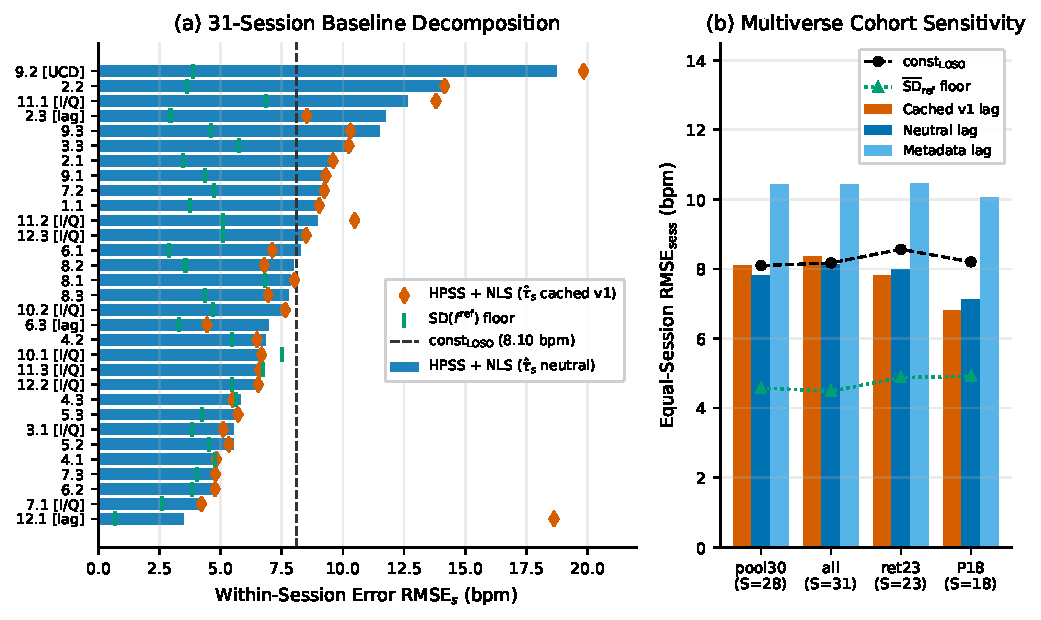
\includegraphics[width=0.92\textwidth]{exp0_session_error_decomposition}
  \caption{Session-wise error under alternative synchronization regimes and local cohort
  definitions. Variation across the panels combines cohort membership, lag, and window validity;
  it should not be read as an isolated causal effect of synchronization.}
  \label{fig:ch3_session_error}
\end{figure}

\section{Reference-channel audit and observed error patterns}
\label{sec:ch3_reference_forensics}

The local EDF contains both a one-hertz \texttt{RespRate} channel and high-rate respiratory trigger
events. These channels represent different constructions of the reference: one is a monitor rate
stream, while the other supports an event-interval estimate. Across 7,101 valid windows, the
1,024-Hz respiratory-trigger rate has a mean signed difference of +2.214 bpm and a mean absolute
difference of 5.175 bpm relative to the one-hertz \texttt{RespRate} channel. The disagreement is not
evidence that either channel is universally correct. A trigger-derived inter-breath rate and a
monitor's smoothed rate can respond differently to pauses, timing, and averaging. It does show
that agreement with the one-hertz channel alone does not fully describe respiratory-event tracking.

The same audit provides a useful channel check: for windows with \texttt{SignalIQ >= 50}, the 1,024-Hz
cardiac R-trigger rate has a 0.935-bpm mean absolute difference from the one-hertz heart-rate
channel across 7,081 windows. This supports the internal consistency of that cardiac trigger
comparison under the stated filter. It does not validate the respiratory trigger as a clinical
ground truth or transfer that validation to the radar estimate.

An inter-trigger gap greater than five seconds flags 1,584 of 7,103 valid windows in the 31-session
neutral-alignment set (22.3\%) and 1,581 of 6,640 windows in \texttt{pool30\_sync} (23.8\%). These are
pause-like intervals defined by the trigger stream. They are not diagnoses of apnea: there is no
clinical adjudication here, and the gating and reference construction affect which intervals are
counted. The distinction matters because an estimator can obtain a lower aggregate error by
rejecting or smoothing windows that contain pauses, even when those intervals may be important to
monitoring.

\begin{figure}[htbp]
  \centering
  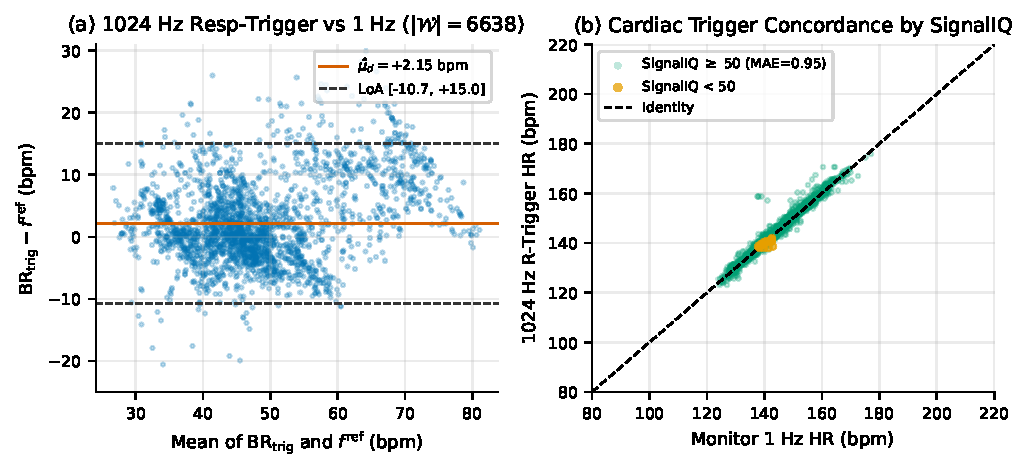
\includegraphics[width=0.92\textwidth]{exp0_edf256_reference_agreement}
  \caption{Agreement between high-rate EDF trigger-derived rates and one-hertz monitor channels.
  The trigger and monitor channels are related references, not interchangeable measurements.}
  \label{fig:ch3_reference_agreement}
\end{figure}

To characterize session error, EXP-0 relates eight telemetry and rate-collision covariates to
excess HPSS error under the shared-lag regime. Here, excess is defined as the session's HPSS RMSE
minus the within-session reference-SD oracle described above. The associations use 28 sessions
from 11 infants and are exploratory Spearman correlations; the listed p-values are nominal and
not adjusted for testing multiple covariates. They identify patterns for follow-up, not causal
effects.

\begin{table}[htbp]
  \centering
  \small
  \caption{Selected exploratory associations with excess session error on \texttt{pool30\_sync}.
  Correlations are across 28 sessions; p-values are nominal and unadjusted.}
  \label{tab:ch3_error_drivers}
  \begin{tabularx}{\textwidth}{@{}Xrrr@{}}
    \toprule
    Session covariate & Spearman $\rho$ with excess error & $p$ & $\rho$ with $\rWithin$ \\
    \midrule
    HR-collision-band window fraction & +0.696 & $<10^{-4}$ & -0.073 \\
    Minimal-movement window fraction & -0.563 & 0.0018 & +0.512 \\
    Windows within 10 bpm of HR/2 & +0.541 & 0.0030 & +0.082 \\
    Respiratory double-octave error fraction & +0.431 & 0.0220 & -0.132 \\
    UCD non-\texttt{ChildPresent} fraction & +0.335 & 0.0810 & -0.112 \\
    \bottomrule
  \end{tabularx}
\end{table}

The strongest positive association is between HR-collision-band windows and excess error. The
negative association with the minimal-movement fraction is consistent with more stable radar
windows being easier to track, but both variables are measured at the session level and can share
other causes. The HR/2 and double-octave patterns are consistent with harmonic ambiguity described
in Chapter~2. The UCD non-child fraction is weaker in this sample and its nominal p-value exceeds
0.05. None of these findings alone shows that cardiac interference, movement, or a device state
caused a specific error. The physics-error and session-decomposition figures are diagnostic
summaries, not interventions.

\begin{figure}[htbp]
  \centering
  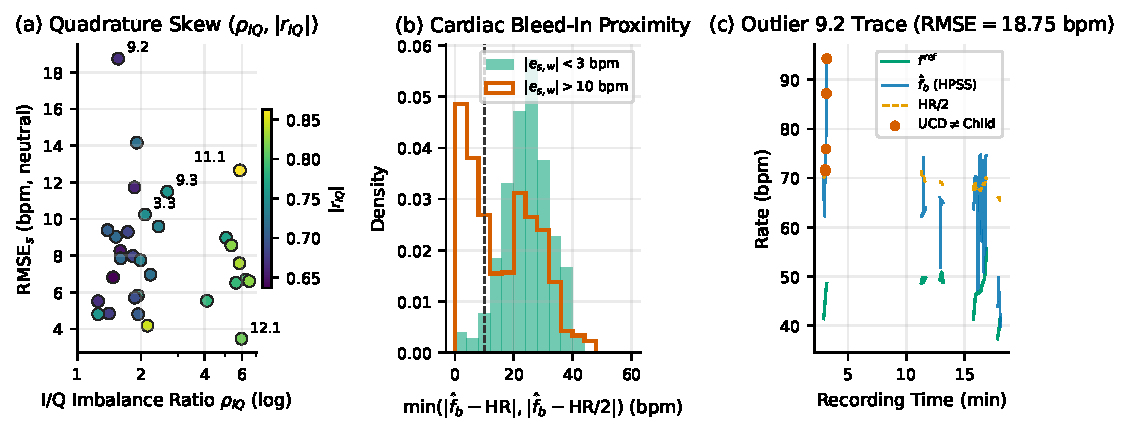
\includegraphics[width=0.92\textwidth]{exp0_physics_error_drivers}
  \caption{Exploratory session-level associations between measured telemetry or rate-collision
  covariates and error. These observational relationships do not identify causal mechanisms.}
  \label{fig:ch3_physics_error}
\end{figure}

Two individual sessions illustrate distinct failure modes that remain after synchronization is
standardized. Session~11.1 has an I/Q standard-deviation ratio of 5.86, absolute I/Q correlation
of 0.863, and clipping in 5.06\% of samples. Its HPSS $\rmseSess$ is 12.65 bpm with the shared
lag, 13.81 bpm under the cached lag, and 16.22 bpm under metadata-only timing. A large spread
imbalance, collinearity, and clipping can make a quadrature trajectory poorly conditioned, but
these measurements do not identify which receiver or motion mechanism dominates the error.

Session~9.2 has an observed mid-session UCD status dropout from \texttt{ChildPresent}. Under the shared
lag its HPSS error is 18.75 bpm; metadata-only timing gives 11.68 bpm. This contrast cautions
against treating the status flag as a sufficient quality score or assuming one lag regime corrects
every session. Telemetry and status fields are contextual indicators, not ground-truth labels for
the failure mechanism.

\section{Stage~0: reconstruction of score-based Viterbi tracking}
\label{sec:ch3_viterbi_methods}

Stage~0 asks whether sequence decoding improves the locked HPSS-NLS baseline and which ingredients
are needed for any improvement. The comparison is performed on \texttt{pool30\_sync}, using the shared
raw-NLS-derived lag and the one-hertz respiratory-rate reference. It contains 28 sessions from 11
infants and 6,640 valid windows. \texttt{A4\_HPSS\_NLS} is the frozen signal-processing anchor. DFT, raw
NLS, and NMF-NLS baselines separate the contributions of a spectral peak, harmonic scoring, and
NMF preprocessing. The B-series explores alternative spectral evidence; the C-series adds
one-dimensional or joint breathing--heart-rate states, harmonic-aware penalties, and
leave-one-patient-out (LOPO) transition selection.

For each window, the tracker receives a score over a discrete breathing-rate grid. The basic
one-dimensional model uses candidate rates from 18 to 90 bpm at 2-bpm spacing. A transition term
penalizes large adjacent rate changes with a Gaussian-shaped log score. The Viterbi recursion
maximizes the summed emission and transition scores over the complete sequence. The two-dimensional
variant adds a heart-rate state on a 90--210 bpm grid and a harmonic-quality term that penalizes
breathing candidates that collide with plausible cardiac harmonics. It is a joint latent-state
decoder; it should not be interpreted as a validated heart-rate output.

The ablations distinguish two design choices that can otherwise be confounded. Unanchored spectral
emissions use broad Welch or harmonic-NLS evidence directly. Anchored emissions use a coarse
autocorrelation estimate to weight harmonic evidence near a local candidate. The latter retains
the temporal optimizer but gives it a physiologically informed local reference. LOPO variants
select transition and emission settings on training patients while holding out the test patient.
The selected parameters are therefore not fitted to that patient's evaluation labels, although
the decoded path itself still uses the full held-out session and is offline.

The anchored harmonic-NLS peak baseline (\texttt{B5a}) reaches 7.701 bpm equal-session RMSE,
compared with 7.817 bpm for \texttt{A4\_HPSS\_NLS}. This modest difference shows that local
anchoring changes the candidate evidence even before sequence decoding. The Viterbi ablations
then test whether temporal structure improves that anchored representation.

\begin{table}[htbp]
  \centering
  \small
  \caption{Representative Stage~0 methods on \texttt{pool30\_sync} with the shared lag. $\Delta$ is
  the change in equal-session RMSE relative to \texttt{A4\_HPSS\_NLS}; negative values favor the method.}
  \label{tab:ch3_viterbi_ladder}
  \begin{tabular}{@{}lrrrrr@{}}
    \toprule
    Method & $\rmseSess$ & $\rmsePool$ & $\accTau{10}$ & $\rWithin$ & $\Delta$ \\
    & bpm & bpm & \% & & bpm \\
    \midrule
    A1 DFT & 11.878 & 11.459 & 65.1 & 0.353 & +4.061 \\
    A2 raw NLS & 8.172 & 8.021 & 77.1 & 0.466 & +0.355 \\
    A3 NMF-NLS & 8.074 & 8.146 & 79.1 & 0.377 & +0.256 \\
    A4 HPSS-NLS & 7.817 & 7.970 & 79.4 & 0.423 & 0.000 \\
    B5a anchored harmonic-NLS peak & 7.701 & 7.887 & 79.3 & 0.431 & -0.116 \\
    C1b 1D Welch Viterbi & 10.109 & 10.219 & 70.7 & 0.361 & +2.292 \\
    C2b 1D HQI Viterbi & 10.077 & 10.160 & 70.4 & 0.369 & +2.259 \\
    C3b joint BR/HR Viterbi & 9.648 & 9.923 & 72.3 & 0.359 & +1.831 \\
    C4b unanchored harmonic-NLS Viterbi & 13.030 & 14.344 & 55.9 & 0.159 & +5.213 \\
    C4c anchored 1D Viterbi & 7.182 & 7.513 & 81.6 & 0.452 & -0.636 \\
    C4d anchored joint Viterbi & 7.036 & 7.306 & 82.0 & 0.471 & -0.782 \\
    C6d LOPO wide anchored Viterbi & 6.877 & 7.205 & 83.7 & 0.456 & -0.941 \\
    \bottomrule
  \end{tabular}
\end{table}

The unanchored sequence models do not improve the baseline. The 1D Welch Viterbi has an equal-
session RMSE of 10.109 bpm, and the joint BR/HR model has 9.648 bpm, both worse than the
7.817-bpm \texttt{A4\_HPSS\_NLS} anchor. Adding unanchored harmonic-NLS evidence alone is not sufficient:
\texttt{C4b} reaches 13.030 bpm. These results oppose the simple hypothesis that a temporal prior or a
larger joint state space automatically resolves harmonic confusion. When the emission surface
places strong mass on a half-rate, double-rate, or cardiac-related candidate, sequence continuity
can preserve the wrong path over time.

Anchoring the harmonic evidence changes the result. Beyond the \texttt{B5a} anchored peak baseline,
\texttt{C4c} reduces $\rmseSess$ to 7.182 bpm, and the joint anchored \texttt{C4d} reaches 7.036
bpm. The \texttt{C6d} LOPO-wide transition variant reaches 6.877
bpm, with a paired mean difference from \texttt{A4} of $-0.941$ bpm. It wins on all 11 patient-level
aggregates; the patient-level Wilcoxon comparison remains significant after the reported Holm
correction ($p_{\mathrm{pat,Holm}}=0.0205$). This is internal evidence for the tested
branch-neutral cohort and reference, not evidence of generalization to an unseen site or bedside
benefit. \texttt{C6e}, the corresponding NMF variant, has a slightly lower point RMSE of 6.826 bpm, but
its result also depends on the incompletely specified local NMF solver and is not the primary
HPSS reconstruction.

The LOPO analysis has a further selection boundary. The wide search evaluates a finite grid of
one- and two-dimensional settings, and \texttt{C6d} selects a boundary-valued configuration in all 11
folds (none is upper-pinned; all are flagged as a boundary selection). This does not invalidate the
held-patient comparison, but it means the grid did not locate an interior optimum. The result is
best read as performance among the prespecified candidates, with transition settings that merit
further search or regularization.

\begin{figure}[htbp]
  \centering
  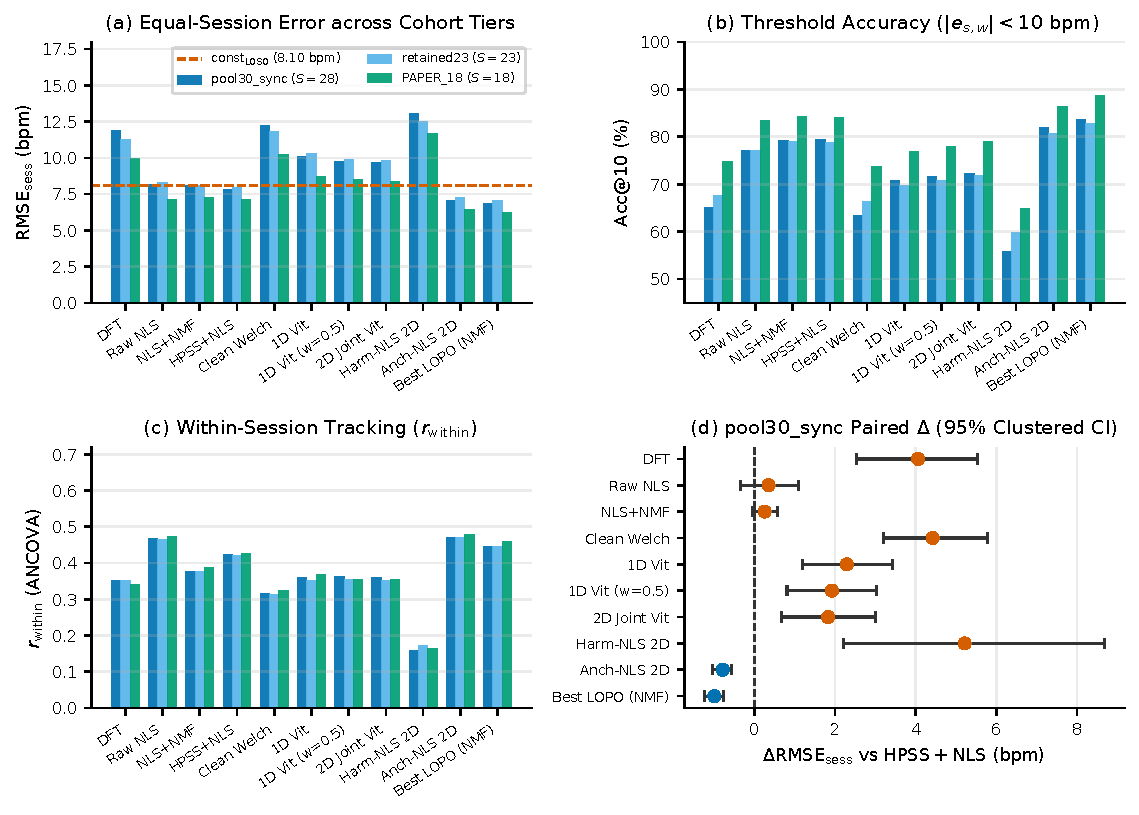
\includegraphics[width=0.92\textwidth]{viterbi_repro_ablation_ladder}
  \caption{Stage~0 ablation ladder. Unanchored sequence decoding degrades the baseline, whereas
  anchored harmonic evidence recovers lower error on the tested local cohort.}
  \label{fig:ch3_ablation_ladder}
\end{figure}

\begin{figure}[htbp]
  \centering
  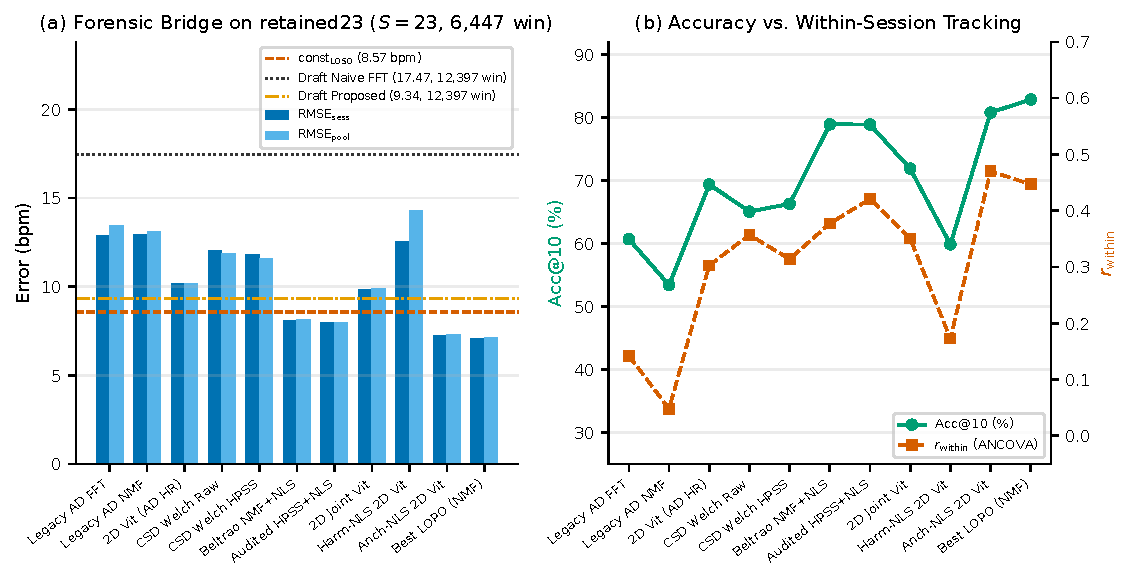
\includegraphics[width=0.92\textwidth]{viterbi_repro_forensic_bridge}
  \caption{Forensic bridge from the signal-processing baseline to Viterbi variants, including
  the role of candidate evidence and temporal structure.}
  \label{fig:ch3_forensic_bridge}
\end{figure}

\section{Agreement, negative controls, and the offline limit}
\label{sec:ch3_viterbi_controls}

RMSE is not a sufficient description of a tracker. A path can reduce average error while losing
dynamic association with the reference, and pooled-window metrics can conceal session-level
disagreement. The reconstructed analysis therefore reports equal-session and pooled RMSE,
within-session correlation, strict-threshold accuracy, and Bland--Altman summaries separately.
On \texttt{PAPER\_18}, the difference between $\rmseSess$ and $\rmsePool$ is about 0.42 bpm for the
cached HPSS baseline, illustrating why the aggregation rule must accompany a result.

The surrogate controls test whether a favorable metric can persist when the temporal or radar
structure is disrupted. In 20 time-shuffled-reference runs, within-session correlations for the
baseline and representative Viterbi methods are approximately zero. In five full-session
phase-scrambled-radar runs, the anchored joint Viterbi likewise has near-zero mean within-session
correlation (approximately $-0.001$), despite a finite aggregate RMSE. Phase scrambling preserves
the session Fourier magnitudes while randomizing phase; it is a stress test of the signal's
temporal structure, not a model of a particular clinical artifact. The near-zero association
shows why a plausible-looking rate range or aggregate error alone cannot establish that a method
is following respiratory information.

A stiff-transition control makes the same point from another direction. With the breathing-rate
transition scale forced to 0.25 bpm, an anchored 2D tracker reports $\rmseSess=6.188$ bpm, lower
than \texttt{C6d}, but its $\rWithin$ is only 0.266. A very strong temporal prior can compress changes
and improve average error on a restricted sample while tracking less of the within-session
variation. This control argues against selecting a tracker from RMSE alone.

Synthetic checks support implementation behavior under constructed conditions, with limits. The
anchored 2D tracker returns the exact 45-bpm state in the stationary 45-bpm/150-bpm-heart-rate
example. In the constructed 35-to-65-bpm chirp with movement and a 150-bpm cardiac component, its
RMSE is approximately 0.326 bpm. These results show that the tested code can resolve those
specified synthetic mixtures; they do not establish that real neonatal signals follow the same
model or that the method handles unmodeled movement and reference error.

The HR component of the joint state was also evaluated against the high-rate R-trigger reference
as a separate output. None of nine cardiac extractors passes the predefined 50\% within-10-bpm
criterion; the best session-averaged result is 39.8\%. Thus, the HR state in the joint decoder is
used as auxiliary evidence for harmonic ambiguity. The present analysis does not validate it as a
clinical heart-rate measurement.

Finally, Stage~0 Viterbi decoding is noncausal. The optimal path is recovered by backtracking from
the final frame, so each estimate can depend on future observations from the full processed
session. The LOPO split protects patient-level parameter selection, but it does not turn this
offline path into a zero-lookahead estimate. The improvements therefore motivate the constrained
causal filters in Chapter~4; they do not demonstrate real-time tracking, alarm latency, or bedside
apnea detection.

\begin{figure}[htbp]
  \centering
  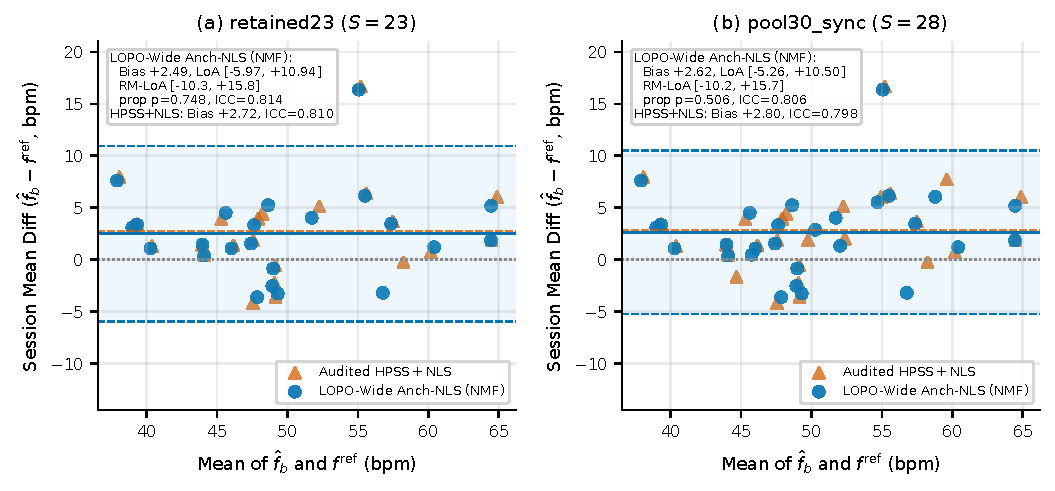
\includegraphics[width=0.92\textwidth]{viterbi_repro_bland_altman}
  \caption{Agreement summaries for representative Stage~0 methods. Limits and bias are shown
  with session structure retained; correlation alone would not characterize this agreement.}
  \label{fig:ch3_bland_altman}
\end{figure}

\begin{figure}[htbp]
  \centering
  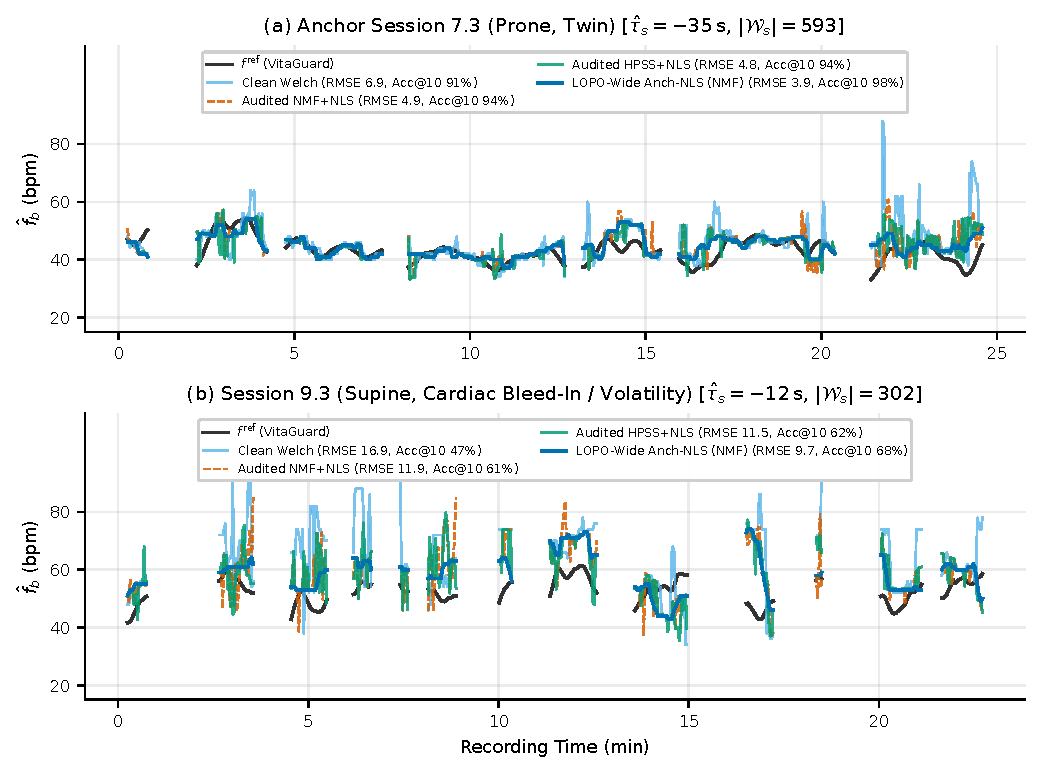
\includegraphics[width=0.92\textwidth]{viterbi_repro_tracking_examples}
  \caption{Example tracking trajectories illustrating candidate selection and temporal
  continuity. These selected sessions illustrate mechanisms and are not a substitute for the
  cohort-level summaries.}
  \label{fig:ch3_tracking_examples}
\end{figure}

\section{Chapter summary}
\label{sec:ch3_summary}

This chapter verified the local baseline caches and reconstructed the main Stage~0 comparisons,
while maintaining the distinction between internal parity and exact paper reproduction. The
reference-assisted shared lag reduces branch-specific alignment differences but does not remove
reference dependence, and lag changes also alter the valid-window denominator. Across the local
cohort variants, session-level error varies with inclusion and synchronization. Exploratory
session correlations point to cardiac-rate collisions and movement-related measures as useful
diagnostic leads, but they do not identify causes. Trigger-versus-monitor disagreement further
shows that the reference itself has a measurement definition and time scale.

The Viterbi ablation gives a more specific methodological result. Unanchored Viterbi and joint
BR/HR decoding worsen the baseline; anchored harmonic emissions recover better internal error,
with the best reported LOPO-wide HPSS model at 6.877 bpm. That result is bounded by 11 infants,
reference-assisted synchronization, boundary selections in every LOPO fold, and offline
infinite-lookahead decoding. The surrogate controls also show that low aggregate error can coexist
with almost no within-session association after signal structure is disrupted. Chapter~4 therefore
tests causal, constrained alternatives and their front-end assumptions, rather than treating the
offline Stage~0 optimum as a deployable monitor.

\chapter{Parsimony and Causal Inductive Bias Across Complexity Rungs}
\label{ch:parsimony_complexity}

The preceding chapter showed that synchronization, reference construction, and spectral
ambiguity all shape respiratory-rate error. This chapter asks how much additional model
complexity is justified once those measurement choices are made explicit. The experiments
progress from small changes to the quadrature front end, through causal and offline temporal
filters, to differentiable hidden-state models and unconstrained neural regressors. The central
comparison is not simply whether a more complex model can lower one RMSE. It is whether a
measured gain survives patient-level evaluation, a second reference definition, physical
perturbation tests, and constraints that prevent the model from relying on absolute-rate
shortcuts.

The primary internal cohort is \texttt{pool30\_sync}, comprising 28 sessions from 11 infants.
The frozen baseline and the Stage~1 and Stage~2 reconstructions use the same shared raw-NLS lag.
Stage~2 models are trained within patient-disjoint leave-one-patient-out (LOPO) folds using only
the monitor's one-hertz respiratory-rate channel. Their predictions are then evaluated against
that channel and against high-rate respiratory triggers. The lag-adjusted trigger evaluation,
called \texttt{Trig -10 s} in the project outputs, compensates for the monitor's observed
approximately ten-second group delay; it is a shared reference-alignment sensitivity, not a
per-model lag optimization. These results remain internal evaluations on one small cohort.
The full Stage~2 audit also retains the recorded-time trigger and the whole-window trigger-count
rate; the principal model table foregrounds the one-hertz and lag-adjusted interval-rate
references.

Figure~\ref{fig:ch4_rungs} summarizes the contrast between structured, rate-equivariant models
and higher-capacity regressors that can exploit absolute-rate correlations.
\begin{figure}[htbp]
\centering
\resizebox{\textwidth}{!}{%
\begin{tikzpicture}[
  x=1cm, y=1cm,
  font=\footnotesize\sffamily,
  >=Stealth,
  physbox/.style={
    draw=oiGreen!80!black, fill=oiSafeBg, rounded corners=3pt,
    thick, align=center, inner sep=6pt
  },
  shortcutbox/.style={
    draw=oiVermilion!85!black, fill=oiWarnBg, rounded corners=3pt,
    thick, align=center, inner sep=6pt
  },
  featbox/.style={
    draw=oiBlue!80!black, fill=oiLightBg, rounded corners=3pt,
    thick, align=center, inner sep=6pt
  },
  statpill/.style={
    draw=oiGray!65, fill=white, rounded corners=2pt,
    thin, align=center, inner sep=5pt, font=\scriptsize\sffamily
  }
]

% Left Input Node centered vertically at y = 3.35
\node[featbox, text width=3.65cm, minimum height=6.40cm] (input) at (1.90, 3.35)
  {\textbf{Folded Harmonic}\\ \textbf{Salience Tensor}\\$\mathbf{\Phi}_t \in \mathbb{R}^{K_q \times d}$\\[7pt]
   $6$ orthogonal channels\\across grid $q\in[18,90]$\,bpm:\\[5pt]
   \scriptsize $P_{\mathrm{clean}}(f),\; P_{\mathrm{clean}}(2f)$\\[2pt]
   $P_{\mathrm{clean}}(3f),\; P_{\mathrm{clean}}(f/2)$\\[2pt]
   $\phi_{\mathrm{anchor}},\; P_{\mathrm{raw}}(f)$\\[8pt]
   \scriptsize $SO(2)\times\mathbb{R}_{>0}$-invariant,\\zero-leakage \texttt{csd()} + HPSS};

% Top Branch: Rung 1 & Rung 2 Equivariant Path (y = 5.45 -> ~0.95 cm clear above bottom box)
\node[physbox, text width=6.35cm, minimum height=2.25cm] (r2) at (7.80, 5.45)
  {\textbf{Rung 1 (3p) \& Rung 2 FilterSafe-8 (8p):}\\
   \textbf{Shift-Equivariant Differentiable 1D-HMM}\\[5pt]
   $\eta_t(q) = \sum_m w_m \Phi_{t,m}(q)$ (zero absolute bin weights)\\
   Exact BPTT Forward--Backward ($\le\num{3.6e-9}$ grad err)\\
   Shift equivariant: $+10\,\mathrm{bpm}$ err $= \SI{1.4e-14}{\bpm}$};

\node[statpill, text width=4.20cm, minimum height=2.25cm, right=0.55cm of r2] (r2res)
  {\textbf{Dual-Reference \& \texttt{L4} Verified}\\[3pt]
   NICU 1\,Hz: $\mathbf{6.849}$ ($p_{\mathrm{Holm}}=\mathbf{0.0117}$)\\
   NICU Trig $-10\,\mathrm{s}$: $\mathbf{8.063}$ ($p_{\mathrm{Holm}}=\mathbf{0.0215}$)\\
   \texttt{gleichauf2024}: $\mathbf{0.0197}$\,bpm, slope $\mathbf{0.9994}$\\
   20\,bpm skirt: $\mathbf{0.0949}$\,bpm\\
   80\,bpm in-band: $\mathbf{0.0089}$\,bpm};

% Bottom Branch: Rung 3 Shortcut Path (y = 1.25)
\node[shortcutbox, text width=6.35cm, minimum height=2.25cm] (r3) at (7.80, 1.25)
  {\textbf{Rung 3 (439--15,817p):}\\
   \textbf{Unconstrained Absolute-Frequency Regressors}\\[5pt]
   \texttt{R3c} Ridge (439p), \texttt{R3b} MLP (15k), \texttt{R3a} TCN (16k)\\
   Break translation symmetry $\implies$ memorize VitaGuard\\
   \SI{10}{\second} trend lag \& training cohort prior ($\sim\SIrange{45}{50}{\bpm}$)};

\node[statpill, text width=4.20cm, minimum height=2.25cm, right=0.55cm of r3] (r3res)
  {\textbf{In-Band Illusion / \texttt{L4} Collapse}\\[3pt]
   NICU 1\,Hz: $5.798$--$6.584$\,bpm (variance $\times 0.52$)\\
   NICU Trig $-10\,\mathrm{s}$: $8.102$--$8.515$ ($p_{\mathrm{Holm}}=1.00$)\\
   \texttt{gleichauf2024}: $\mathbf{3.18}$--$\mathbf{3.64}$\,bpm (slope $0.709$)\\
   20\,bpm skirt: $\mathbf{11.78}$--$\mathbf{32.70}$\,bpm collapse};

% Connections
\draw[->, very thick, oiGreen!80!black] (input.east) |- (r2.west);
\draw[->, very thick, oiGreen!80!black] (r2.east) -- (r2res.west);
\draw[->, very thick, oiVermilion!85!black] (input.east) |- (r3.west);
\draw[->, very thick, oiVermilion!85!black] (r3.east) -- (r3res.west);

\end{tikzpicture}%
}
\caption[Physical Equivariance vs.\ Shortcut Complexity Architecture]{Architectural contrast across the Stage~2 Complexity Ladder (\texttt{Rung 1--3}): weight-shared zero-offset 1D-HMM operators (\texttt{R1a}, \texttt{R2e FilterSafe-8}) preserve exact translation equivariance and transfer zero-touch to \texttt{gleichauf2024}, whereas unconstrained absolute-frequency regressors (\texttt{R3c}, \texttt{R3b}, \texttt{R3a}) memorize VitaGuard \SI{1}{\hertz} smoothing and the NICU rate prior.}
\label{fig:ch4_rungs}
\end{figure}


\section{Two references and the measurement-time problem}
\label{sec:ch4_references}

The Stage~1 benchmark carries forward the distinction between the one-hertz
\texttt{RespRate} monitor stream and the high-rate respiratory trigger series. In the primary
cohort, the trigger-derived interval rate differs from the monitor rate by a mean of
$+2.15$~bpm when pooled across windows and $+1.65$~bpm when averaged equally across sessions,
with differences defined as trigger rate minus monitor rate.
Its window-level mean absolute difference is $5.03$~bpm (Table~\ref{tab:ch4_dual_reference}), and its within-session association with
the monitor is $\rWithin=0.606$ at zero offset. These are comparisons between two measurement
constructions, not an adjudication that either one is a universal ground truth.

The trigger interval rate is computed from inter-trigger gaps after excluding gaps longer than
five seconds. Consequently, windows containing pauses can report the rate of the breaths that
occurred while omitting the time spent without a breath. A whole-window count rate,
\texttt{br\_trig\_count\_bpm}, makes the opposite choice and includes the pauses in its
denominator. Relative to the one-hertz rate, the count-based estimate has a pooled difference of
$-7.08$~bpm overall and $-13.52$~bpm in windows containing a greater-than-five-second gap.
These pause-like intervals are not clinically adjudicated apnea events. The contrast shows that
the target rate depends on the reference definition, especially during quiet intervals.

\begin{table}[htbp]
  \centering
  \footnotesize
  \setlength{\tabcolsep}{4.5pt}
  \caption{One-hertz monitor and respiratory-trigger comparison under the shared Stage~1
  alignment. Differences are trigger rate minus monitor rate; the trigger interval estimator
  excludes inter-trigger gaps longer than five seconds.}
  \label{tab:ch4_dual_reference}
  \begin{tabularx}{\textwidth}{@{}>{\raggedright\arraybackslash}Xrrrrr@{}}
    \toprule
    Cohort & Sessions & Monitor win & Trigger win & Mean diff (sess / pool) & MAE (pool) \\
    \midrule
    \texttt{pool30\_sync} & 28 & 6,640 & 6,638 & $+1.65 / +2.15$ & 5.03 \\
    \texttt{retained23} & 23 & 6,447 & 6,445 & $+1.64 / +2.13$ & 5.01 \\
    \texttt{PAPER\_18} & 18 & 5,466 & 5,466 & $+1.39 / +1.69$ & 4.65 \\
    \texttt{all\_paired} & 31 & 7,103 & 7,101 & $+1.69 / +2.21$ & 5.18 \\
    \bottomrule
  \end{tabularx}
\end{table}

The two rate streams also differ in time. Across the 28 primary-cohort sessions, their
within-session correlation rises from $0.606$ at zero lag to $0.706$ at the audited ten-second
offset between the streams. This pattern is consistent with an
effective monitor group delay in these recordings. It is not an independent measurement of a
hardware specification. The causal forward estimate in Stage~1 adds its own delay: R1a's peak
association occurs at $+6$~s against the one-hertz stream and $+16$~s against the trigger stream.
The offline R1f smoother peaks at $+4$~s and $+14$~s, respectively. Results against the trigger
at zero offset therefore mix rate-estimation error with both monitor and estimator timing.

For that reason, the experiments report both the trigger at its recorded timing and the shared
\texttt{Trig -10 s} evaluation. The latter helps separate the common monitor delay from differences
between models. Neither alignment can remove the reference's pause definition or turn these
monitor-derived measurements into clinically adjudicated labels.

\section{Stage 1 front-end parsimony}
\label{sec:ch4_frontend_parsimony}

\subsection{WP1: I/Q preprocessing gate}
\label{sec:ch4_wp1}

The locked front end starts with mean-centered complex demodulation of the I/Q samples and the
frozen signal-processing chain. WP1 tested whether clipping repair or symmetric whitening could
improve that reference without adding avoidable axis dependence. The six alternatives were
channel-wise or joint interpolation at ADC rail hits, three symmetric whitening strengths, and a
combined clipping-and-whitening treatment. All were evaluated against both the monitor and the
high-rate trigger reference.

None of the six alternatives has patient-level Holm-adjusted support on either reference
(Table~\ref{tab:ch4_wp1}): all adjusted $p$-values are $1.000$. The largest point improvement
among the whitening variants on the one-hertz reference is small relative to between-session
variation and is not reproduced as a supported result on the trigger reference. The sentinel
sessions reinforce the concern. For example, the heavily clipped sentinel Session~2.3
(18.5\% ADC rail clipping) moves from 11.73~bpm under the locked method to 13.95--14.31~bpm
for standalone whitening (13.71~bpm under combined clipping-and-whitening \texttt{F3});
Session~11.1 moves from 12.65~bpm to 12.78--13.21~bpm for standalone whitening (12.98~bpm under
\texttt{F3}). In addition, channel-wise interpolation and the combined channel-wise
procedure depend on the I/Q axes and do not preserve the same unconditional rotation invariance
as the locked complex representation.

\begin{table}[htbp]
  \centering
  \footnotesize
  \setlength{\tabcolsep}{4pt}
  \caption{WP1 front-end ablation on \texttt{pool30\_sync}. Every candidate's patient-level
  Holm-adjusted comparison with the locked anchor is non-significant on both references.}
  \label{tab:ch4_wp1}
  \begin{tabularx}{\textwidth}{@{}>{\raggedright\arraybackslash}p{4.1cm}rrr>{\raggedright\arraybackslash}p{2.2cm}>{\raggedright\arraybackslash}X@{}}
    \toprule
    Method & $\rmseSess$ (1\,Hz) & $\Delta_{1\mathrm{Hz}}$ & $\rmseSess$ (Trig) & $p_{\mathrm{pat,Holm}}$ (1\,Hz / Trig) & Note \\
    \midrule
    F0 locked CSD & 7.817 & anchor & 8.968 & -- & Locked reference \\
    F1a channel clip repair & 7.832 & $+0.014$ & 8.963 & 1.000 / 1.000 & Axis-dependent mask \\
    F1b joint clip repair & 7.831 & $+0.014$ & 8.966 & 1.000 / 1.000 & Conditional shared mask \\
    F2a sym.\ whitening ($\lambda_{\mathrm{wh}}=0.05$) & 7.804 & $-0.014$ & 8.949 & 1.000 / 1.000 & No supported gain \\
    F2b sym.\ whitening ($\lambda_{\mathrm{wh}}=0.10$) & 7.833 & $+0.015$ & 8.976 & 1.000 / 1.000 & No supported gain \\
    F2c sym.\ whitening ($\lambda_{\mathrm{wh}}=0.25$) & 7.689 & $-0.128$ & 8.804 & 1.000 / 1.000 & Sentinel degradation \\
    F3 clipping + whitening & 7.812 & $-0.006$ & 8.935 & 1.000 / 1.000 & Axis-dependent clipping \\
    \bottomrule
  \end{tabularx}
\end{table}

The Gate~G1 decision is therefore \texttt{RETAIN\_F0\_CSD\_LOCKED}. This is a parsimony
decision under the registered statistical and symmetry criteria, not a claim that the current
front end is optimal for every receiver fault. A preprocessing step should be retained only when
it delivers a reproducible benefit without introducing a new failure mode.

\subsection{WP2: the HPSS lookahead--equivalence trade-off}
\label{sec:ch4_wp2}

WP2 varied the short-time Fourier transform (STFT) window, frequency restriction, and amount of
future context used by harmonic--percussive source separation (HPSS). The locked reference,
\texttt{H0}, uses the rectangular $48/16/256$ STFT configuration and the existing 64-tap
zero-phase Kaiser FIR bandpass over $[0.30,3.00]$~Hz with $\kaiserBeta=6.5$. The bandpass is the
project's locked filter throughout Stages~0--4; it is not a Butterworth alternative. The HPSS
windowing variants range from three seconds of STFT lookahead to zero seconds
(Table~\ref{tab:ch4_wp2}).

\begin{table}[htbp]
  \centering
  \footnotesize
  \setlength{\tabcolsep}{4.5pt}
  \caption{WP2 HPSS window and lookahead ablation. Runtime is HPSS milliseconds per window;
  the error columns use the monitor and the recorded-time respiratory trigger.}
  \label{tab:ch4_wp2}
  \begin{tabularx}{\textwidth}{@{}>{\raggedright\arraybackslash}Xrrrrr@{}}
    \toprule
    Method & STFT lookahead & ms/win & Speedup & $\rmseSess$ (1\,Hz) & $\rmseSess$ (Trig 0\,s) \\
    \midrule
    H0 locked rectangular, full band & 3\,s & 3.47 & 1.00$\times$ & 7.817 & 8.968 \\
    H1 Hann COLA, full band & 3\,s & 3.69 & 0.94$\times$ & 7.999 & 9.113 \\
    H2 Hann COLA, in band & 3\,s & 2.38 & 1.46$\times$ & 8.068 & 9.146 \\
    H3 causal Hann COLA, 2-hop context & 2\,s & 2.37 & 1.46$\times$ & 8.121 & 9.074 \\
    H4 causal Hann COLA, 1-hop context & 1\,s & 2.35 & 1.47$\times$ & 8.176 & 9.235 \\
    H5 causal Hann COLA, no STFT lookahead & 0\,s & 2.35 & 1.47$\times$ & 8.267 & 9.398 \\
    H6 causal rectangular, no STFT lookahead & 0\,s & 3.41 & 1.02$\times$ & 8.079 & 9.303 \\
    \bottomrule
  \end{tabularx}
\end{table}

The faster in-band variants trade some accuracy for runtime. More importantly, the zero-STFT-
lookahead candidates do not meet the prespecified $\pm0.50$~bpm equivalence criterion against
\texttt{H0} on both references and at both session and patient levels. For \texttt{H5}, the
session/patient TOST $p$-values are $0.414/0.519$ on the one-hertz reference and $0.412/0.431$
on the trigger reference. For \texttt{H6}, the corresponding values are $0.053/0.027$ and
$0.231/0.186$; equivalence fails at least one required level. The point estimate for \texttt{H5}
is only 0.449~bpm worse than the locked anchor, but a point estimate inside the margin is not
enough to establish equivalence.

Gate~G2 therefore retains \texttt{H0\_Locked\_Rect\_Full\_L3} as the primary front end and carries
\texttt{H5} as a zero-STFT-lookahead ablation. This result sets an important boundary for
subsequent use of the word causal: the Rung~1 and Rung~2 state decoders can use no future
sequence windows while still receiving features from an HPSS front end with three seconds of
STFT lookahead. For \texttt{H5}, zero lookahead refers only to HPSS/STFT frame context. The
evaluated path also uses block-level envelope normalization and a zero-phase outer bandpass, so
it does not establish a fully frame-causal, zero-latency pipeline. It does not pass the
equivalence gate.

\section{Rung 1: temporal structure and the causality frontier}
\label{sec:ch4_rung1}

Rung~1 adds a small temporal model to the locked HPSS-NLS estimates. Its three-parameter
forward-MMSE form updates a breathing-rate posterior over the $[18,90]$~bpm candidate grid using the current
window's evidence and a transition model. At each step it reports the posterior mean without
backtracking through future windows. The MAP variant reports the most probable state, while the
fixed-lag and offline variants deliberately use increasing amounts of future context. The
comparison in Table~\ref{tab:ch4_rung1} tests both whether temporal continuity is useful and how
much latency is required to obtain it.

\begin{table}[htbp]
  \centering
  \footnotesize
  \setlength{\tabcolsep}{4pt}
  \caption{Rung~1 causality frontier on \texttt{pool30\_sync}. Block lookahead describes sequence
  decoding; STFT lookahead describes HPSS frame context, not total pipeline latency. The H0-backed
  rows retain three seconds of STFT lookahead; $\accTau{10}$ reports the equal-session mean of
  per-session strict $|e_{s,w}|<10$~bpm accuracy on the one-hertz reference.}
  \label{tab:ch4_rung1}
  \begin{tabularx}{\textwidth}{@{}>{\raggedright\arraybackslash}Xrrrrrr@{}}
    \toprule
    Method & Params & Blk / STFT & $\rmseSess$ (1\,Hz) & $\accTau{10}$ (1\,Hz) & $\rWithin$ (1\,Hz) & $\rmseSess$ (Trig 0\,s) \\
    \midrule
    R0 locked HPSS-NLS & 0 & 0 / 3\,s & 7.817 & 79.4\% & 0.423 & 8.968 \\
    R1a forward MMSE & 3 & 0 / 3\,s & 6.990 & 82.6\% & 0.454 & 8.624 \\
    R1b forward MAP & 3 & 0 / 3\,s & 7.458 & 80.0\% & 0.389 & 8.987 \\
    R1c fixed-lag MMSE & 3 & 4 / 3\,s & 6.893 & 83.0\% & 0.473 & 8.402 \\
    R1d fixed-lag MMSE & 3 & 8 / 3\,s & 6.787 & 83.4\% & 0.479 & 8.246 \\
    R1e fixed-lag MMSE & 3 & 16 / 3\,s & 6.759 & 83.8\% & 0.484 & 8.083 \\
    R1f offline FB MMSE & 3 & $\infty$ / 3\,s & 6.395 & 86.2\% & 0.454 & 7.789 \\
    R1g offline Viterbi & 2 & $\infty$ / 3\,s & 6.498 & 85.2\% & 0.439 & 7.876 \\
    R1h H5 zero-STFT MMSE & 3 & 0 / 0\,s & 7.136 & 82.6\% & 0.396 & 8.864 \\
    R1i H6 zero-STFT MMSE & 3 & 0 / 0\,s & 7.119 & 82.6\% & 0.392 & 8.917 \\
    \bottomrule
  \end{tabularx}
\end{table}

The forward-MMSE estimate improves equal-session RMSE from 7.817 to 6.990~bpm against the
one-hertz reference, with $\rWithin=0.454$. Its recorded-time trigger RMSE is 8.624~bpm. Allowing
fixed lag improves the point estimates further, reaching 6.759~bpm at 16~s, while full
forward--backward smoothing reaches 6.395~bpm. These offline results are useful upper-context
comparators, not online alternatives: they use future windows and cannot be emitted at the time
of measurement. The forward filter's improvement over R0 is also not a clinical performance
claim; the trigger timing and pause definition still affect the measured error.

The R1a--R1g paired audit illustrates the uncertainty at this cohort size. R1a's RMSE is
0.493~bpm higher than offline Viterbi under the one-hertz reference; its patient-level Holm
adjusted $p$-value is $0.0957$. Against the recorded-time trigger, the difference is
$+0.748$~bpm and the adjusted patient-level $p$-value is $0.0078$. The offline advantage is
therefore clearer on the physical trigger at zero offset, where filter and monitor delays both
affect agreement. It should not be interpreted as an equal-latency comparison.

Two controls test whether the forward filter is merely producing a smooth, inertial trace. First,
the shifted-grid midpoint audit compares candidate ranges $[18,90]$ and $[18,120]$~bpm on five
sessions. The legacy wide-transition, high-floor filter (8~bpm transition width and 0.05 uniform floor) changes its bias by $+0.26$~bpm, and a memoryless naive
MMSE estimator changes by $+2.82$~bpm. The equivariant forward-MMSE and forward--backward
operators show $+0.00$~bpm shift. Second, in five radar phase-scramble runs, the R1a
within-session correlation falls from $0.454$ to $0.006$ and its RMSE rises from 6.990 to
8.513~bpm. The scrambled input retains Fourier magnitude while losing the original temporal
phase structure. These checks support the intended response to signal structure; they do not
prove that all real-world failures are represented by the surrogate.

\section{Rungs 2 and 3: structured learning versus shortcut capacity}
\label{sec:ch4_complexity}

Stage~2 compares a compact differentiable hidden Markov model (HMM) with substantially larger
regressors. The HMM assigns each candidate respiratory rate a shared emission score derived from
six salience channels: clean-signal power at the fundamental and harmonics, a subharmonic cue, a
coarse autocorrelation anchor, and raw-signal fundamental power. Rung~2 then combines those
scores with a symmetric transition matrix built from a mixture of slow and jump components.
The transition model contains no global uniform component, and the emission weights do not
depend on the absolute rate bin. This structure makes the operator translation-equivariant over
the tested interior grid and discourages a learned preference for one absolute breathing rate.
Differentiable sequence models and their use in structured prediction provide methodological
precedent for this design \citep{mensch2018differentiable,riou2023pesto}.

The primary Rung~2 model, \texttt{R2e}, has eight learned parameters. It uses only three
passband-safe channels---clean fundamental power, the autocorrelation anchor, and raw
fundamental power---along with two symmetric smoothing taps and three transition parameters.
Restricting the evidence to these channels avoids relying on harmonic bins that cross the
locked $0.30$--$3.00$~Hz filter boundaries as the candidate rate changes. \texttt{R2a} uses all
six channels with eleven parameters; \texttt{R2b} uses a 43-parameter nonlinear residual model.
The offline Rung~2 models use the same emissions with future-window smoothing.

Rung~3 consists of a 439-parameter ridge regressor, a 14,593-parameter spectral multilayer
perceptron, and a 15,817-parameter causal temporal convolutional network. These models can fit
more flexible mappings from the training salience to rate, but they have no explicit
rate-translation equivariance constraint. They are therefore informative shortcut-learning
foils: a low in-distribution error may reflect monitor smoothing, the training cohort's rate
distribution, or other stable correlations rather than a representation that transfers when the
rate itself changes \citep{geirhos2020shortcut}.

All models are trained within patient-disjoint LOPO folds using only \texttt{br\_1hz\_30s}. The
one-hertz results are therefore the training-reference evaluation; the recorded-time and
lag-adjusted trigger results are blind reference evaluations. Table~\ref{tab:ch4_complexity_ladder} reports equal-session and
window-pooled RMSE for both references, within-session association, and the equal-session mean
of the per-session prediction-to-reference standard-deviation ratio. A ratio below one means
that, on average across sessions, the predictions vary less than the reference; it can
accompany a favorable average error when the estimator compresses the dynamic range.

\begin{table}[htbp]
  \centering
  \scriptsize
  \setlength{\tabcolsep}{3.5pt}
  \caption{Stage~2 complexity ladder on \texttt{pool30\_sync}. Lookahead is block-decoder
  lookahead / HPSS STFT frame lookahead in seconds; the latter is not total pipeline latency.
  The SD-ratio column gives equal-session mean prediction-to-reference standard-deviation
  ratios for 1\,Hz and lag-adjusted trigger (\texttt{T10}).}
  \label{tab:ch4_complexity_ladder}
  \begin{tabularx}{\textwidth}{@{}>{\raggedright\arraybackslash}Xrcc rrr c rrr@{}}
    \toprule
    & & & \multicolumn{3}{c}{\textbf{1\,Hz Monitor Reference}} & & \multicolumn{3}{c}{\textbf{Trig $-10$\,s Reference}} \\
    \cmidrule(lr){4-6} \cmidrule(l){8-10}
    Model & Params & Blk/STFT & $\rmseSess$ & $\rmsePool$ & $\rWithin$ & SD (1\,Hz / T10) & $\rmseSess$ & $\rmsePool$ & $\rWithin$ \\
    \midrule
    R0 locked & 0 & 0 / 3 & 7.817 & 7.970 & 0.423 & 1.66 / 0.99 & 8.727 & 8.579 & 0.402 \\
    R1a forward MMSE & 3 & 0 / 3 & 6.990 & 7.337 & 0.454 & 1.36 / 0.82 & 8.197 & 8.299 & 0.408 \\
    R1f offline FB & 3 & $\infty$ / 3 & 6.395 & 6.745 & 0.454 & 1.16 / 0.70 & 7.597 & 7.722 & 0.430 \\
    R1g offline Viterbi & 2 & $\infty$ / 3 & 6.498 & 6.913 & 0.439 & 1.20 / 0.73 & 7.715 & 7.924 & 0.408 \\
    R2e causal FilterSafe-8 & 8 & 0 / 3 & 6.849 & 7.186 & 0.465 & 1.36 / 0.82 & 8.063 & 7.969 & 0.441 \\
    R2a causal linear & 11 & 0 / 3 & 6.870 & 7.340 & 0.496 & 1.40 / 0.84 & 8.350 & 8.672 & 0.455 \\
    R2b causal MLP & 43 & 0 / 3 & 6.991 & 7.423 & 0.477 & 1.36 / 0.82 & 8.502 & 8.829 & 0.424 \\
    R2f offline FilterSafe-8 & 8 & $\infty$ / 3 & 6.847 & 7.184 & 0.462 & 1.29 / 0.79 & 7.879 & 7.944 & 0.436 \\
    R2c offline linear & 11 & $\infty$ / 3 & 6.941 & 7.225 & 0.444 & 1.32 / 0.79 & 8.197 & 8.210 & 0.427 \\
    R2d H5 zero-STFT HMM & 11 & 0 / 0 & 7.115 & 7.320 & 0.437 & 1.50 / 0.87 & 8.578 & 8.364 & 0.409 \\
    R3c spectral ridge & 439 & 0 / 3 & 5.798 & 6.785 & 0.490 & 0.88 / 0.55 & 8.102 & 8.724 & 0.425 \\
    R3b spectral MLP & 14,593 & 0 / 3 & 6.584 & 6.863 & 0.481 & 1.35 / 0.82 & 8.515 & 8.652 & 0.412 \\
    R3a causal TCN & 15,817 & 0 / 3 & 6.075 & 6.906 & 0.466 & 0.84 / 0.52 & 8.498 & 8.829 & 0.404 \\
    \bottomrule
  \end{tabularx}
\end{table}

The unadjusted one-hertz ranking favors the more flexible Rung~3 models: R3c reaches
5.798~bpm and R3a 6.075~bpm, compared with 6.849~bpm for R2e. That ordering changes against
the lag-adjusted physical trigger. R2e reaches 8.063~bpm, R3c 8.102~bpm, R3a 8.498~bpm, and
R3b 8.515~bpm. Relative to the one-hertz results, the R3c and R3a predictions also retain only
$0.55$ and $0.52$ of the trigger-reference standard deviation. The combination of an attractive
training-reference RMSE, reduced prediction spread, and a weaker result under the second
reference is consistent with shortcut dependence; the table alone does not prove the causal
mechanism for any individual model.

The capacity comparison also reflects differences in the fitting protocol. For the LOPO scores in
Table~\ref{tab:ch4_complexity_ladder}, every outer fold excludes its test infant. R3a and R3b use
one additional, fold-specific inner-validation infant for model selection, leaving nine infants
for network fitting; the validation infant rotates across folds. R3c and the R2 models use all ten
outer-training infants. Separately, the full-cohort foils frozen for Stage~4 use Patient~12 as the
R3a/R3b validation infant, leaving ten infants for fitting, while R3c and R2 use all eleven. Those
full-cohort refits do not generate the LOPO scores in the table. The Rung~3 results are useful as
shortcut stress tests, but neither comparison isolates parameter count from training-data access.

\begin{table}[htbp]
  \centering
  \small
  \caption{Patient-level paired comparisons for the eight-parameter R2e model. Negative
  differences favor R2e. Holm adjustment is applied within the prespecified comparison family.}
  \label{tab:ch4_r2e_inference}
  \begin{tabularx}{\textwidth}{@{}lXrrr@{}}
    \toprule
    Contrast & Reference & Mean difference [95\% CI] (bpm) & Patient wins & $p_{\mathrm{pat,Holm}}$ \\
    \midrule
    R2e vs.\ R0 & 1~Hz monitor & $-0.969\;[-1.135,-0.803]$ & 11/11 & 0.0117 \\
    R2e vs.\ R0 & Trig $-10$~s & $-0.663\;[-0.883,-0.446]$ & 10/11 & 0.0215 \\
    R2e vs.\ R1a & 1~Hz monitor & $-0.142\;[-0.335,+0.035]$ & 9/11 & 0.6641 \\
    R2e vs.\ R1a & Trig $-10$~s & $-0.134\;[-0.497,+0.166]$ & 7/11 & 1.0000 \\
    \bottomrule
  \end{tabularx}
\end{table}

R2e is the only causal architecture in this comparison that passes patient-level Holm correction
against R0 on both the one-hertz and lag-adjusted trigger references
(Table~\ref{tab:ch4_r2e_inference}). Its mean paired differences
are $-0.969$~bpm and $-0.663$~bpm, respectively. This supports R2e over the zero-parameter
baseline within the stated evaluation. It does not show that eight parameters outperform the
three-parameter R1a forward filter: R2e's patient-level adjusted $p$-values against R1a are
$0.6641$ and $1.0000$. On the one-hertz reference, the prespecified $\pm0.50$~bpm TOST supports
equivalence between R2e and R1a at session and patient levels; the corresponding patient-level
equivalence test does not pass for the lag-adjusted trigger. The defensible conclusion is that
the compact structured model improves on R0 across the two references, while the local data do
not establish a reliable gain over the simpler causal R1a filter.

The patient-level Holm-adjusted comparisons of the Rung~3 foils with R0 sharpen this distinction.
On the one-hertz reference, the adjusted $p$-values are $0.0342$ for R3a, $0.0586$ for R3c, and
$0.1289$ for R3b. On the lag-adjusted trigger, all three are $1.0000$; their patient win counts
are 8/11, 8/11, and 6/11, respectively. Thus R3a's one-hertz result does not reproduce as
patient-level evidence against R0 under the second reference.

On the recorded-time trigger, R2e's $\rmseSess$ is 8.473~bpm, compared with 8.968~bpm for R0,
8.624~bpm for R1a, and 8.255~bpm for R3c. These zero-offset comparisons are affected by the
observed monitor delay and the causal filter's group delay. The adjusted trigger comparisons are
therefore reported alongside them rather than substituted for them
(Figure~\ref{fig:ch4_complexity_ladder}).

\begin{figure}[htbp]
  \centering
  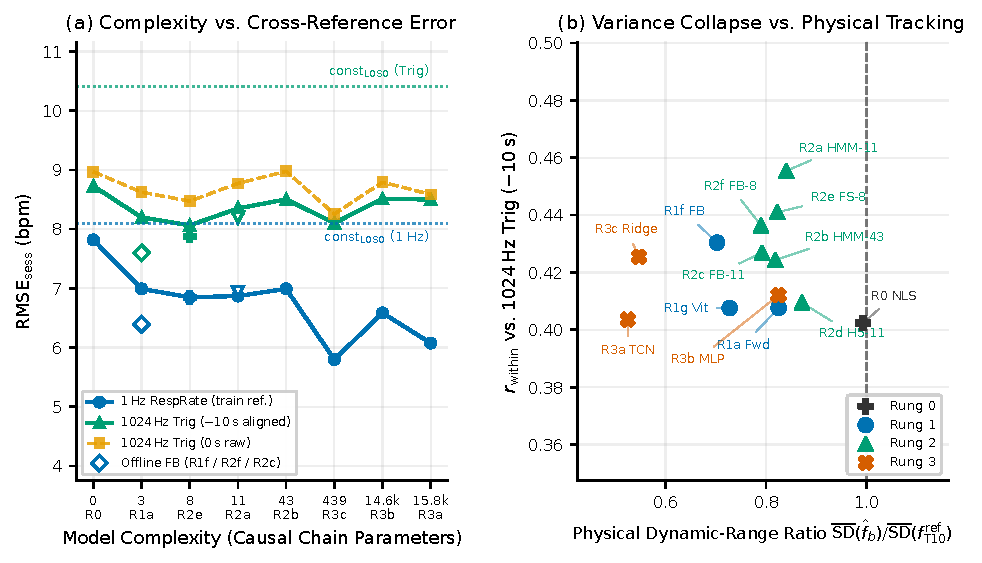
\includegraphics[width=0.94\textwidth]{stage2_complexity_ladder}
  \caption{Four-rung comparison across the training-reference and lag-adjusted trigger
  evaluations. Low one-hertz error from a higher-capacity model does not by itself establish
  transfer to the physical trigger reference.}
  \label{fig:ch4_complexity_ladder}
\end{figure}

\section{Monitor delay, shortcut controls, and physical perturbations}
\label{sec:ch4_controls}

\subsection{Lag profile and the shared trigger correction}
\label{sec:ch4_lag}

In addition to the Stage~2 $[-16,+16]$~s within-session correlation profiles, an independent
post-freeze lag sweep shifts the trigger reference from $-20$ to $+20$~s using the same offset
for each model. Five of the six unshifted models---R0, R1a, R2e, R3c, and R3b---reach their
minimum error or maximum $\rWithin$ at an offset between $+8$ and $+10$~s. For example, R2e
changes from 8.473~bpm at the recorded trigger timing to 8.063~bpm at the project-defined
\texttt{Trig -10 s} alignment, while R1a changes from 8.624 to 8.197~bpm. The common optimum
across architectures is evidence against a model-specific lag search as the explanation for the
observed shift. It is consistent with an effective delay in the monitor reference. The lag
sweep remains observational and cannot separate every source of timing error.

This timing correction is not a learned parameter and is not selected independently for each
held-out infant. It should nevertheless be read as a sensitivity analysis because the trigger and
monitor streams encode different rate definitions, particularly in pause-containing windows.

\subsection{Invariance, causality, gradients, and cache checks}
\label{sec:ch4_implementation_checks}

The structured models were checked against several implementation-level controls. On an
interior rate grid, the Rung~2 operators respond to a rigid $+10$~bpm translation with
numerical error at or below $1.42\times10^{-14}$~bpm for R2e, $7.11\times10^{-15}$~bpm for
R2a, and zero at reported precision for R2b. Under the clinical $[18,90]$~bpm grid
frequency-shift audit ($36\to46$~bpm rigid salience translation), the maximum absolute errors
are $1.20\times10^{-7}$~bpm for R2e, $3.18\times10^{-5}$~bpm for R2a, and
$4.29\times10^{-5}$~bpm for R2b, whereas the absolute-frequency R3c, R3b, and R3a foils show
errors of $3.01$, $5.66$, and $8.86$~bpm. In a separate candidate-grid expansion audit comparing
$[18,90]$ against $[18,120]$~bpm for the flexible-grid Rung~2 decoders, the mean bias shifts
by $0.0000$~bpm for R2e, $0.0188$~bpm for R2a, and $0.0163$~bpm for R2b (the fixed 73-bin
Rung~3 regressors are not defined on the expanded 103-bin grid). On the separate 24~GHz
waveform probe, which changes the input from 36 to 46~bpm, the structured R2e and R2a outputs
change by 9.987 and 10.001~bpm, close to the imposed shift of 10~bpm. The unconstrained R3c,
R3b, and R3a changes are 6.523, 15.043, and 5.465~bpm.

Random future perturbations produce zero reported output difference for the causal forward
decoders and the causal TCN. This is a sequence-level statement about future windows. For
H0-backed models, it does not remove the three-second STFT lookahead described above. The
H5-based R2d ablation removes HPSS/STFT future-frame context, but its block-level normalization
and zero-phase outer bandpass mean that the $0/0$ lookahead entry is not a claim of frame-causal,
zero-latency end-to-end processing. Its one-hertz RMSE is 7.115~bpm, compared with 6.849~bpm for
H0-backed R2e. Because the front end and model both change, this is a bundled comparison, not an
isolated causal effect of STFT lookahead.

Finite-difference checks of the differentiable training gradients found maximum absolute
discrepancies of $4.77\times10^{-9}$ for the tested HMM parameters and
$4.50\times10^{-7}$ for the tested TCN coordinates. The Stage~2 salience extraction was also
recomputed on eight stratified windows from each of 31 session caches: all 248 comparisons
matched the stored features at zero maximum absolute difference for both the H0 and H5 paths.
These audits support implementation fidelity for the tested code and inputs; they do not
validate the model's clinical use.

\subsection{Phase scrambling and synthetic rate sweeps}
\label{sec:ch4_synthetic}

The five-seed phase-scramble control tests whether models continue to follow the reference after
the temporal phase structure of the radar waveform is randomized. For R2e, the one-hertz
$\rmseSess$ rises from 6.849 to $8.361\pm0.105$~bpm, while $\rWithin$ falls from 0.465 to
$-0.006$. The R3 models also show near-zero scrambled within-session correlations. The control
therefore detects dependence on real signal structure in this test, but it is not sufficient to
rule out shortcut learning in the unperturbed recordings.

Synthetic frequency sweeps provide a different test: can the learned mapping follow rates that
were not selected from the NICU cohort's observed distribution? Across stationary 28, 35, 50,
65, and 80~bpm signals and a 30-to-75~bpm chirp (Table~\ref{tab:ch4_synthetic_sweep};
Figure~\ref{fig:ch4_synthetic_sweep}), the passband-safe R2e has low stationary MAE, from 0.01
to 0.04~bpm. The unconstrained R3 errors vary substantially with rate. R3c,
for example, has 7.51~bpm MAE at 28~bpm and 11.18~bpm at 80~bpm; the TCN has 12.45 and
11.14~bpm errors at those rates. These are controlled synthetic signals, so the results
demonstrate behavior under specified mixtures rather than a guarantee for real infants.

\begin{table}[htbp]
  \centering
  \small
  \caption{Zero-touch synthetic frequency sweep. Values are mean absolute error for stationary
  signals and RMSE for the 30-to-75~bpm chirp.}
  \label{tab:ch4_synthetic_sweep}
  \begin{tabular}{@{}lrrrrrr@{}}
    \toprule
    Method & 28~bpm & 35~bpm & 50~bpm & 65~bpm & 80~bpm & Chirp RMSE \\
    \midrule
    R2e FilterSafe-8 & 0.04 & 0.01 & 0.03 & 0.01 & 0.01 & 2.37 \\
    R2a linear HMM & 0.00 & 0.00 & 0.00 & 0.01 & 0.04 & 2.06 \\
    R3c spectral ridge & 7.51 & 5.27 & 2.01 & 3.04 & 11.18 & 2.50 \\
    R3b spectral MLP & 6.64 & 2.88 & 5.43 & 4.81 & 4.28 & 4.15 \\
    R3a causal TCN & 12.45 & 6.06 & 2.80 & 5.81 & 11.14 & 4.99 \\
    \bottomrule
  \end{tabular}
\end{table}

The separate 20~bpm filter-edge diagnostic must not be folded into the 28--80~bpm sweep.
At 20~bpm, the fundamental lies close to the low-frequency skirt of the locked double-pass
Kaiser filter, and the local synthetic test gives 20.00~bpm MAE for R2e and 20.06~bpm for R0.
This exposes a front-end limitation near the passband edge, even though the passband-safe model
performs well over the prespecified 28--80~bpm sweep. The test is not evidence that R2e can
reliably track every rate near the nominal 18~bpm cutoff. It is distinct from the external
20~bpm transfer scenario summarized in Figure~\ref{fig:ch4_rungs} and evaluated in Chapter~6:
that scenario uses a different data source and processing path, so the two results are not
directly interchangeable.

\begin{figure}[htbp]
  \centering
  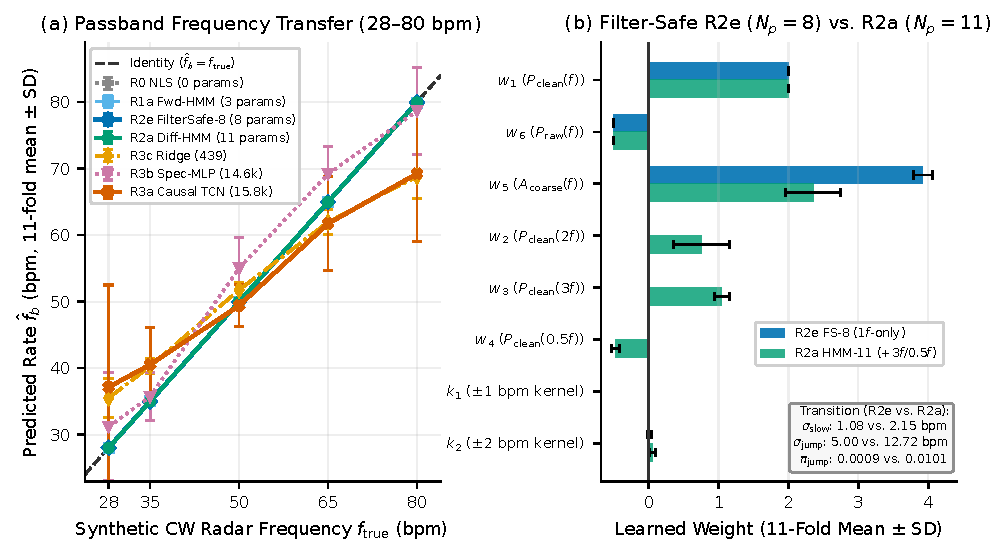
\includegraphics[width=0.94\textwidth]{stage2_synthetic_sweep_and_weights}
  \caption{Passband synthetic rate-sweep results (28--80~bpm) and interpretable Rung~2 weights.
  The frequency sweep reveals rate-dependent errors in unconstrained regressors; the separate
  20~bpm Kaiser low-edge diagnostic is reported in the text.}
  \label{fig:ch4_synthetic_sweep}
\end{figure}

\section{Chapter summary}
\label{sec:ch4_summary}

The Stage~1 gates favor retaining the existing front end: none of the six WP1 I/Q preprocessing
variants shows an adjusted patient-level gain, and the zero-STFT-lookahead HPSS variants do not
establish equivalence to the locked reference. The resulting Rung~1 forward-MMSE filter improves
the one-hertz point estimate without using future sequence windows, while the offline smoothers
show how additional future context can lower error at the cost of latency. The H0-backed causal
decoders still inherit three seconds of STFT lookahead. H5 removes that HPSS/STFT context in its
ablation, but its blockwise normalization and zero-phase filtering also rule out describing the
evaluated path as fully frame-causal and zero-latency.

Across the Stage~2 ladder, the eight-parameter R2e improves on the zero-parameter R0 baseline
with patient-level Holm support against both the one-hertz and lag-adjusted trigger references.
The comparison with the three-parameter R1a filter, however, is Holm-non-significant. Larger
Rung~3 models can rank well against the training reference but show compressed prediction spread,
weaker physical-trigger performance, and poor transfer across synthetic rates. The causal
structured model is therefore a compact, internally supported candidate, not a clinically
validated monitor. The reference delay, pause-dependent target definition, STFT lookahead, and
20~bpm filter-edge behavior remain explicit boundaries. Chapter~5 builds on this model while
examining whether its posterior uncertainty can support selective prediction without hiding
pause-like intervals.

\chapter{Selective Uncertainty, Quiet-Apnea Safety, and Finite-\texorpdfstring{$K$}{K} Conformal Audit}
\label{ch:uncertainty_conformal}

\section{Motivation and evaluation scope}

Chapter~4 established R2e as the strongest internally supported candidate in the present evaluation, while showing that its gain over simpler R1a is not sufficiently robust to support a claim of general superiority. Neither result is a clinical validation. This chapter asks whether an estimator can identify unreliable predictions, abstain selectively without disproportionately suppressing quiet-apnea windows, and produce prediction intervals whose finite-sample limits are explicit.

The Stage~3 uncertainty and conformal audit (\texttt{WP3}/\texttt{WP4}) uses the frozen \texttt{pool30\_sync} cohort: 28 synchronous sessions from 11 infants. The primary waveform reference is the 1~Hz monitor-training reference; the shared Trig~$-10$~s blind sensitivity analysis follows Chapter~4. Windows are repeated observations nested within sessions and infants. Window-level summaries are descriptive; patient-level comparisons are more relevant to consistency across infants. This small internal cohort is not an external clinical validation set.

\section{Uncertainty scores and selective prediction}
\label{sec:ch5_selective}

\subsection{Scores and operating rule}

The eight proxies are U1, posterior entropy; U2, posterior standard deviation; U3, clean-waveform spectral entropy; U4, raw-waveform spectral entropy; U5, harmonic deficit; U6a, additive signal-quality index (SQI); U6b, geometric SQI; and U6c, a five-parameter SQI calibrated under leave-one-patient-out (LOPO) evaluation. U1--U5 are parameter-free scores. U6a is a fixed additive combination of normalized posterior standard deviation, posterior entropy, and the OOD barrier (weights 0.45, 0.35, and 0.20); U6b combines the same components through an equal-exponent geometric confidence score. Specifically, with $u_1 \in [0,1]$ denoting normalized posterior Shannon entropy, $u_2 \in [0,1]$ posterior standard deviation normalized by the standard deviation of the uniform 1~bpm respiratory-rate grid and clipped to $[0,1]$, and $h_{\mathrm{mix}}$ causal temporal mixture spectral entropy, the barrier is $b_{\mathrm{ood}}=\operatorname{clip}((h_{\mathrm{mix}}-\tau_{\mathrm{ood}})/(1-\tau_{\mathrm{ood}}),0,1)$. The uncertainty scores are $u_{6a}=\operatorname{clip}(0.45u_2+0.35u_1+0.20b_{\mathrm{ood}},0,1)$ and $u_{6b}=1-\big[(1-u_2)(1-u_1)(1-b_{\mathrm{ood}})\big]^{1/3}$. The weights and exponents are not fitted, but both composites use the fixed $\tau_{\mathrm{ood}}=0.90$ and a three-hop (6~s) causal history. The cutoff and history rule are design choices, so the composites are not threshold-free. U6c fits five simplex-normalized non-negative weights over U1--U5 via regularized non-negative least squares with training-fold standardization. U2 provides a simple posterior-spread reference without fitted parameters or an additional OOD barrier cutoff.

Selective prediction ranks windows from least to most uncertain, retains the lower-uncertainty fraction, and rejects the rest. Coverage, $\covLevel$, is swept from 0.50 to 1.00. Risk is RMSE among retained windows. Excess area under the risk--coverage curve ($\eaurcMetric$) is normalized by the 0.50 coverage span and measured relative to the constant random-abstention (full-coverage) baseline rather than the oracle; a negative value therefore indicates lower average risk than full coverage in bpm under this convention. The 80\% point is reported separately as a concrete operating point.

At 1~Hz, U2 yielded E-AURC $-0.2454$ [$-0.4069,-0.1168$]. At 80\% coverage, RMSE changed from 6.8486 to 6.6890~bpm, and 10 of 11 infants had lower patient-level risk. The raw patient-level comparison was $p=0.0098$; after Holm correction it was $p=0.0781$. For Trig~$-10$~s, U2 yielded E-AURC $-0.2929$ [$-0.4555,-0.1436$], and RMSE changed from 8.0634 to 7.8798~bpm. Nine of 11 infants improved; raw $p=0.0244$ and Holm-adjusted $p=0.1953$. Point estimates favor U2, but neither comparison remains statistically significant after the reported multiplicity correction.

Across all eight proxies, session-level RMSE decreased at the 80\% operating point, but the patient-level evidence was weaker: no patient-level comparison remained significant after Holm correction. Several spectral and harmonic E-AURC intervals include zero, and U6c's 1~Hz interval includes zero as well. Table~\ref{tab:ch5_selective_results} gives the complete proxy-by-reference results, and Figure~\ref{fig:ch5_risk_coverage_safety} summarizes the selective risk--coverage and pause-safety trade-off; U6c also fails the pause-safety criterion described below.

\begin{table}[htbp]
\centering
\scriptsize
\setlength{\tabcolsep}{4pt}
\caption{Selective-prediction results for all eight R2e uncertainty proxies. RMSE is the session-macro risk at full and 80\% coverage; E-AURC is the session-level area difference in bpm with its 95\% CI in brackets. Infant counts are patient-level wins for the reference shown in that column. Patient-level $p$-values are shown as raw/Holm-adjusted across the eight proxies within each reference.}
\label{tab:ch5_selective_results}
\begin{tabularx}{\textwidth}{@{}>{\raggedright\arraybackslash}p{0.8cm}>{\raggedright\arraybackslash}p{2.35cm}>{\raggedright\arraybackslash}X >{\raggedright\arraybackslash}X@{}}
\toprule
Proxy & Score & 1~Hz monitor-training reference & Trig~$-10$~s sensitivity \\
\midrule
U1 & Posterior entropy & RMSE $6.8486 \rightarrow 6.6230$~bpm; E-AURC $-0.2194$ [$-0.4015,-0.0742$]; 9/11 improved; $p=0.0244$, Holm $=0.1709$ & RMSE $8.0634 \rightarrow 7.7841$~bpm; E-AURC $-0.2530$ [$-0.4175,-0.1152$]; 9/11 improved; $p=0.1016$, Holm $=0.6094$ \\
\addlinespace[2pt]
U2 & Posterior SD & RMSE $6.8486 \rightarrow 6.6890$~bpm; E-AURC $-0.2454$ [$-0.4069,-0.1168$]; 10/11 improved; $p=0.0098$, Holm $=0.0781$ & RMSE $8.0634 \rightarrow 7.8798$~bpm; E-AURC $-0.2929$ [$-0.4555,-0.1436$]; 9/11 improved; $p=0.0244$, Holm $=0.1953$ \\
\addlinespace[2pt]
U3 & Clean spectral entropy & RMSE $6.8486 \rightarrow 6.6782$~bpm; E-AURC $-0.1776$ [$-0.5126,+0.1624$]; 8/11 improved; $p=0.2783$, Holm $=1.0000$ & RMSE $8.0634 \rightarrow 7.7517$~bpm; E-AURC $-0.3735$ [$-0.7584,+0.0533$]; 9/11 improved; $p=0.2061$, Holm $=0.6152$ \\
\addlinespace[2pt]
U4 & Raw spectral entropy & RMSE $6.8486 \rightarrow 6.6637$~bpm; E-AURC $-0.1946$ [$-0.4495,+0.1038$]; 9/11 improved; $p=0.2783$, Holm $=1.0000$ & RMSE $8.0634 \rightarrow 7.7150$~bpm; E-AURC $-0.3604$ [$-0.7117,+0.0341$]; 7/11 improved; $p=0.2061$, Holm $=0.6152$ \\
\addlinespace[2pt]
U5 & Harmonic deficit & RMSE $6.8486 \rightarrow 6.6544$~bpm; E-AURC $-0.2284$ [$-0.5454,+0.0453$]; 8/11 improved; $p=0.2402$, Holm $=1.0000$ & RMSE $8.0634 \rightarrow 7.7899$~bpm; E-AURC $-0.3752$ [$-0.6950,-0.0570$]; 8/11 improved; $p=0.1230$, Holm $=0.6152$ \\
\addlinespace[2pt]
U6a & Additive SQI & RMSE $6.8486 \rightarrow 6.5920$~bpm; E-AURC $-0.2448$ [$-0.4842,-0.0496$]; 8/11 improved; $p=0.0830$, Holm $=0.4980$ & RMSE $8.0634 \rightarrow 7.7694$~bpm; E-AURC $-0.3009$ [$-0.5284,-0.1014$]; 9/11 improved; $p=0.0830$, Holm $=0.5811$ \\
\addlinespace[2pt]
U6b & Geometric SQI & RMSE $6.8486 \rightarrow 6.5956$~bpm; E-AURC $-0.2398$ [$-0.4982,-0.0257$]; 8/11 improved; $p=0.2402$, Holm $=1.0000$ & RMSE $8.0634 \rightarrow 7.7569$~bpm; E-AURC $-0.2932$ [$-0.5500,-0.0699$]; 8/11 improved; $p=0.1230$, Holm $=0.6152$ \\
\addlinespace[2pt]
U6c & Five-parameter SQI & RMSE $6.8486 \rightarrow 6.6145$~bpm; E-AURC $-0.2688$ [$-0.5926,+0.0266$]; 8/11 improved; $p=0.2402$, Holm $=1.0000$ & RMSE $8.0634 \rightarrow 7.6774$~bpm; E-AURC $-0.4218$ [$-0.7514,-0.0828$]; 8/11 improved; $p=0.1230$, Holm $=0.6152$ \\
\bottomrule
\end{tabularx}
\end{table}

The HQI coding audit qualifies U5. In the implemented harmonic-quality calculation, the fundamental-peak bins ($\pm 2$~bpm around the fundamental peak) are included inside both the peak-plus-harmonic numerator term and the total-passband denominator term, double-counting those bins in the denominator and compressing raw values below $0.5$. The observed HQI range was [0.0655, 0.4351], versus [0.0700, 0.7193] under non-overlapping accounting. Rank ordering was nearly identical (Spearman $\rho=0.999945$), and U5's 1~Hz E-AURC on R2e changed by only $+0.0032$~bpm (from $-0.2284$ to $-0.2253$~bpm). This sensitivity result shows little change in ranking for this cohort; it does not make the definitions interchangeable.

Sequence-level future-window perturbations produced zero output difference for all eight proxies in the tested implementation. This does not establish zero end-to-end latency: the H0 front end retains a 3~s short-time Fourier transform look-ahead, as described in Chapter~4. The result therefore does not establish a fully causal, zero-look-ahead system.

\begin{figure}[htbp]
\centering
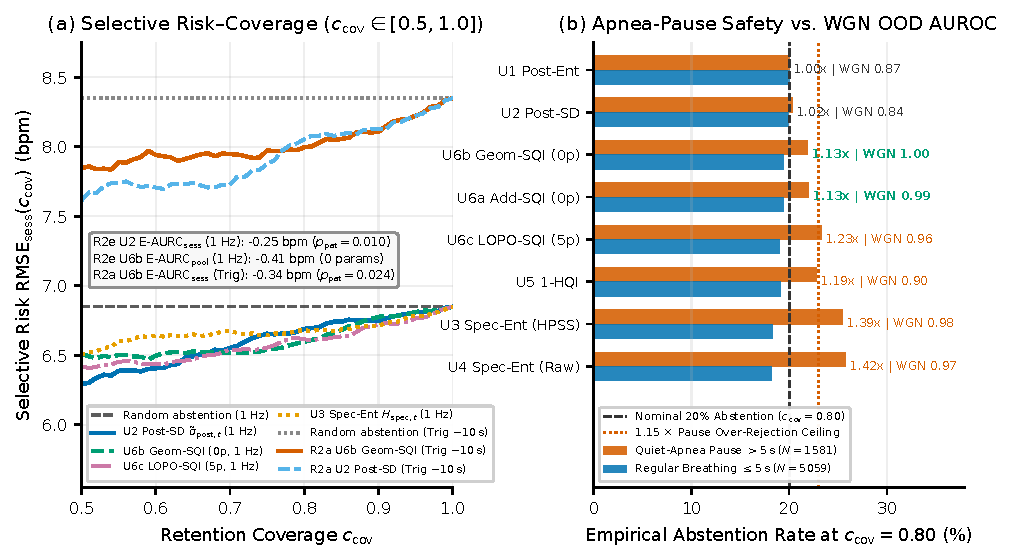
\includegraphics[width=0.95\textwidth]{stage3_risk_coverage_and_apnea_safety}
\caption{Frozen Stage~3 risk--coverage and apnea-safety summary. Panel~(a) plots equal-session selective risk $\rmseSess(\covLevel)$ for R2e on the 1~Hz reference alongside overlaid R2a curves on the lag-adjusted trigger sensitivity (\texttt{Trig~$-10$~s}); the frozen legend shorthand ``(0p)'' / ``0~params'' on U6a and U6b denotes zero fitted weights (with fixed $\tau_{\mathrm{ood}}=0.90$ and 3-hop history). Panel~(b) compares R2e pooled abstention rates at $\covLevel=0.80$ in pause ($>5$~s, $N=1{,}581$) versus regular ($\le 5$~s, $N=5{,}059$) windows alongside WGN OOD AUROC.}
\label{fig:ch5_risk_coverage_safety}
\end{figure}

\section{Quiet-apnea safety and OOD detection}
\label{sec:ch5_safety}

The pause-safety audit included 1,581 pause windows and 5,059 regular windows; pause windows were identified by an inter-breath gap greater than 5.0~s. These operational strata are not clinically adjudicated apnea events. At 80\% overall coverage, pause rejection ratio is the rejection rate among pause windows divided by the rejection rate among regular windows. The project's diagnostic limit is a ratio no greater than 1.15. This is an internal engineering criterion, not a clinical threshold.

U2 had a pause-rejection ratio of 1.0200 under global pooled 80\% thresholding and 1.0645 under within-session 80\% thresholding (pooled across sessions after per-session ranking). Its WGN OOD AUROC was 0.8406, with a false-positive rate (FPR) of 0.4515 at 95\% true-positive rate (TPR). Table~\ref{tab:ch5_pause_ood} shows the central trade-off across all eight proxies: a score can detect synthetic noise strongly while also rejecting pause windows more often.

\begin{table}[htbp]
\centering
\footnotesize
\caption{Pause-safety and synthetic WGN OOD audit for all eight R2e uncertainty proxies at 80\% overall coverage. Pause ratio reports global-threshold (pooled) / within-session-threshold rejection risk ratios (diagnostic ceiling $\le 1.15$).}
\label{tab:ch5_pause_ood}
\begin{tabularx}{\textwidth}{@{}>{\raggedright\arraybackslash}Xrrr@{}}
\toprule
Proxy & Pause rejection ratio (pool / sess) & WGN AUROC & WGN FPR at 95\% TPR \\
\midrule
U1 posterior entropy & 0.9992 / 1.0432 & 0.8698 & 0.4407 \\
U2 posterior SD & 1.0200 / 1.0645 & 0.8406 & 0.4515 \\
U3 clean spectral entropy & 1.3941 / 1.1342 & 0.9796 & 0.0926 \\
U4 raw spectral entropy & 1.4191 / 1.2292 & 0.9735 & 0.1014 \\
U5 harmonic deficit & 1.1946 / 1.1971 & 0.8982 & 0.2714 \\
U6a additive SQI & 1.1319 / 1.1122 & 0.9935 & 0.0191 \\
U6b geometric SQI & 1.1275 / 1.1209 & 0.9986 & 0.0036 \\
U6c calibrated SQI & 1.2266 / 1.1971 & 0.9635 & 0.1209 \\
\bottomrule
\end{tabularx}
\end{table}

At the selected $\tau_{\mathrm{ood}}=0.90$ with three-hop history, U6b met the project's pause-ratio limit and separated the tested WGN condition (AUROC 0.9986; FPR 0.0036 at 95\% TPR). The audit also recorded no barrier triggers for the tested synthetic shallow-breathing conditions down to 0.2~mm and 10~dB (28, 45, and 75~bpm). In auxiliary targeted non-child (UCD) audits, blind waveform-only U6b reached AUROC 0.6235 across all 261 partial-window ($>0\%$) non-child windows and AUROC 0.9055 on the 32 majority-corrupted ($\ge 50\%$) windows, whereas deterministic firmware telemetry gating yielded AUROC 1.0. The Stage~3 invariance check on H5 reported a maximum numerical difference of $8.88\times10^{-16}$ under the tested $O(2)\times\mathbb{R}_{>0}$ transformations; on the primary H0-backed R2e path, post-freeze fuzzing verified $SO(2)\times\mathbb{R}_{>0}$ invariance to $\le 2.22\times10^{-16}$ for U6b alongside an I/Q-swap Nyquist clamping residual of $\le 5.24\times10^{-6}$. These results concern specified synthetic or targeted audit conditions; they do not validate performance across external hospitals, devices, patient populations, or naturally occurring failure modes.

Table~\ref{tab:ch5_u6b_sensitivity} reports the full tested cutoff and history sensitivity for U6b. The pooled pause ratio is evaluated at 80\% coverage; patient wins and $p$-values are for the 1~Hz selective-risk comparison. These raw $p$-values are not adjusted across the cutoff and history configurations and are exploratory.

\begin{table}[htbp]
\centering
\footnotesize
\caption{U6b cutoff and history sensitivity on R2e. E-AURC is in bpm; pause ratio is pooled at 80\% coverage. WGN results are AUROC and FPR at 95\% TPR. ``None'' means no entropy cutoff ($b_{\mathrm{ood}}=h_{\mathrm{mix}}$). Patient $p$-values are raw and unadjusted across configurations.}
\label{tab:ch5_u6b_sensitivity}
\begin{tabularx}{\textwidth}{@{}cc>{\raggedright\arraybackslash}Xrr@{}}
\toprule
History hops & $\tau_{\mathrm{ood}}$ & E-AURC; wins; raw patient $p$ & Pause ratio & WGN AUROC / FPR \\
\midrule
3 & None & $-0.2396$; 8/11; 0.3203 & 1.3160 (fail) & 0.9990 / 0.0030 \\
3 & 0.75 & $-0.2365$; 8/11; 0.3203 & 1.3160 (fail) & 0.9990 / 0.0030 \\
3 & 0.80 & $-0.2307$; 8/11; 0.3203 & 1.3160 (fail) & 0.9990 / 0.0030 \\
3 & 0.85 & $-0.2308$; 8/11; 0.3203 & 1.3016 (fail) & 0.9990 / 0.0030 \\
3 & 0.88 & $-0.2424$; 8/11; 0.2783 & 1.1765 (fail) & 0.9989 / 0.0030 \\
3 & 0.90 (locked) & $-0.2398$; 8/11; 0.2402 & 1.1275 (pass) & 0.9986 / 0.0036 \\
3 & 0.92 & $-0.2282$; 9/11; 0.0322 & 1.0284 (pass) & 0.9968 / 0.0075 \\
3 & 0.95 & $-0.2194$; 9/11; 0.0244 & 1.0075 (pass) & 0.9482 / 0.2444 \\
0 & 0.90 & $-0.2329$; 9/11; 0.0420 & 1.0666 (pass) & 0.9509 / 0.1645 \\
1 & 0.90 & $-0.2376$; 8/11; 0.0830 & 1.1099 (pass) & 0.9955 / 0.0139 \\
2 & 0.90 & $-0.2403$; 8/11; 0.1230 & 1.1275 (pass) & 0.9979 / 0.0060 \\
5 & 0.90 & $-0.2240$; 8/11; 0.4131 & 1.1275 (pass) & 0.9989 / 0.0018 \\
\bottomrule
\end{tabularx}
\end{table}

Among the listed three-hop cutoff points, 0.90 and 0.92 met both the pause ratio limit and the project's WGN AUROC criterion of 0.95. At 0.95, pause rejection was lowest but WGN AUROC fell below 0.95. Cutoffs of 0.88 and below failed the pause limit despite strong WGN detection. At $\tau_{\mathrm{ood}}=0.90$, all tested histories (0, 1, 2, 3, and 5 hops) met both project criteria; the zero-hop AUROC of 0.9509 was only marginally above the threshold. This supports reporting the locked three-hop setting as a measured operating point, not as a universally optimal cutoff.

This is the pause-safety/OOD trade-off in the present evaluation. Lowering the barrier cutoff increases rejection of high-entropy windows: that strengthens WGN detection but can reject quiet breathing pauses disproportionately. A plausible signal-level explanation is that a pause weakens periodic harmonic structure and can make the normalized spectrum flatter, raising spectral entropy; this is an interpretation of the observed score behavior, not a clinical characterization of the pauses. At three-hop history, the NICU causal temporal mixture spectral-entropy 95th percentile was 0.9130, compared with 0.9498 at the WGN 5th percentile. Their proximity makes the operating point sensitive to threshold choice. U6b at 0.90 is an empirically selected, data-motivated cutoff for this cohort and these audits. It is not threshold-free or a universally safe setting. U6c's pause ratio of 1.2266 exceeds the project's 1.15 limit despite favorable risk--coverage point estimates.

\section{Finite-\texorpdfstring{$K$}{K} conformal calibration}
\label{sec:ch5_conformal}

\subsection{Calibration units and finite-rank limit}

Each LOPO fold has $K_{\mathrm{cal}}=10$ calibration patients because one of the 11 infants is held out. For a split-conformal order statistic at miscoverage level $\alpha$, the finite-sample rank is
\[
i_{\alpha}=\left\lceil (K_{\mathrm{cal}}+1)(1-\alpha)\right\rceil.
\]
At a nominal 95\% target, $\alpha=0.05$ and $i_{\alpha}=\lceil 11(0.95)\rceil=11$, which exceeds the ten available calibration patients. Thus the patient-level C4 and C5 intervals are infinite (vacuous) at this target. C1--C3 return finite intervals by using window- or session-level calibration units, but those constructions do not provide the same patient-level exchangeability basis. With ten calibration patients, the smallest nonzero attainable tail probability is $1/(K_{\mathrm{cal}}+1)=1/11\approx0.0909$. At least 19 calibration patients are needed for this rank construction to return a finite patient-level interval at a 95\% target.

This is a resolution limit imposed by the number of independent calibration units. Adding windows from the same infants does not create more independent patients. The audit compared five constructions:
\begin{itemize}
\item C1 randomly splits windows 50/50 between calibration and evaluation. Windows from the same patients may enter both partitions, creating patient-level leakage.
\item C2 uses LOPO but treats pooled windows as exchangeability units. Repeated windows from an infant are correlated, so this unit does not match the data structure.
\item C3 computes within-session quantiles and an outer session-level order statistic, using sessions as calibration units even though multiple sessions remain clustered within patients.
\item C4 first computes within-patient absolute-error quantiles and then applies an outer patient-level quantile.
\item C5 follows the same two-level structure after scaling absolute error by posterior standard deviation floored at 1~bpm, then rescales the calibrated radius.
\end{itemize}

C4 and C5 are local two-level patient-quantile procedures motivated by hierarchical conformal work. They do not automatically inherit a theorem that guarantees distribution-free coverage for this cohort. When the same nominal level is used at both levels, the simple hierarchical bound is $(1-\alpha)^2$, rather than $1-\alpha$, under the required hierarchical assumptions. In Dunn et al.'s supervised new-group setting, CDF pooling is asymptotically valid for continuous outcomes, single subsampling has finite-sample $1-\alpha$ validity, and repeated subsampling (aggregating $p$-values into a single set) has a finite-sample $1-2\alpha$ lower bound \citep{dunn2023distribution}. The head-to-head table evaluates Dunn et al.'s CDF-pooling rule and a $B=200$ Monte Carlo average of single-draw subsampling (replicating single-draw subsampling 200 times and averaging coverage and width rather than constructing a $p$-value-averaged repeated-subsampling set); empirical averages here should not be confused with a finite-sample guarantee on our cohort. Dunn's guarantees also rely on the relevant within-group and between-group exchangeability assumptions. Our 30~s windows overlap by 93.3\% and are serially dependent, so these methods are empirical comparators here; no distribution-free guarantee is claimed for their local use or for C4/C5.

\subsection{Empirical coverage across target levels}

Table~\ref{tab:ch5_conformal_all} and Figure~\ref{fig:ch5_finite_k_conformal} report frozen R2e LOPO results for the 1~Hz monitor-training reference. Mean and minimum coverage are calculated across the 11 held-out patients; undercovered counts patients below the nominal target. Pooled coverage and mean full interval width show how aggregate behavior can differ from patient-level behavior. At the 95\% target, C4 and C5 return vacuous intervals, so their empirical coverage is 1 and their mean width is infinite. The other values are empirical outcomes on this cohort, not guarantees for future infants.

\begin{table}[htbp]
\centering
\footnotesize
\setlength{\tabcolsep}{4pt}
\caption{R2e LOPO conformal audit for the 1~Hz monitor-training reference by nominal coverage target. Width is mean full interval width in bpm. C4 and C5 are vacuous at the 95\% target because the finite-sample rank is unavailable.}
\label{tab:ch5_conformal_all}
\begin{tabularx}{\textwidth}{@{}cc>{\raggedleft\arraybackslash}Xrrrr@{}}
\toprule
Method & Target & Mean patient cov & Minimum & Undercovered & Pooled cov & Mean width \\
\midrule
C1 & 0.95 & 0.933 & 0.789 & 5 & 0.947 & 29.12 \\
C2 & 0.95 & 0.934 & 0.785 & 4 & 0.946 & 29.32 \\
C3 & 0.95 & 0.995 & 0.968 & 0 & 0.995 & 50.60 \\
C4 & 0.95 & 1.000 & 1.000 & 0 & 1.000 & $\infty$ \\
C5 & 0.95 & 1.000 & 1.000 & 0 & 1.000 & $\infty$ \\
\midrule
C1 & 0.90 & 0.892 & 0.677 & 4 & 0.909 & 23.62 \\
C2 & 0.90 & 0.881 & 0.623 & 4 & 0.898 & 23.23 \\
C3 & 0.90 & 0.975 & 0.875 & 1 & 0.978 & 38.51 \\
C4 & 0.90 & 0.976 & 0.875 & 1 & 0.979 & 38.84 \\
C5 & 0.90 & 0.963 & 0.847 & 1 & 0.970 & 39.18 \\
\midrule
C1 & 0.80 & 0.798 & 0.477 & 5 & 0.812 & 17.30 \\
C2 & 0.80 & 0.772 & 0.398 & 5 & 0.795 & 17.00 \\
C3 & 0.80 & 0.885 & 0.632 & 2 & 0.904 & 23.83 \\
C4 & 0.80 & 0.895 & 0.551 & 2 & 0.919 & 25.57 \\
C5 & 0.80 & 0.864 & 0.586 & 2 & 0.881 & 24.02 \\
\midrule
C1 & 0.70 & 0.692 & 0.350 & 6 & 0.703 & 13.14 \\
C2 & 0.70 & 0.677 & 0.292 & 5 & 0.697 & 13.09 \\
C3 & 0.70 & 0.758 & 0.366 & 4 & 0.780 & 16.41 \\
C4 & 0.70 & 0.760 & 0.389 & 3 & 0.783 & 16.27 \\
C5 & 0.70 & 0.766 & 0.440 & 3 & 0.777 & 17.62 \\
\bottomrule
\end{tabularx}
\end{table}

At the 80\% target, C1 pooled coverage is 0.812 while its minimum patient coverage is 0.477; C2 pooled coverage is 0.795 and minimum patient coverage is 0.398. Pooled or cohort averages therefore do not describe how intervals behave for every infant. C3--C5 have higher mean patient coverage at this target, but minimum patient coverage remains between 0.551 and 0.632, and their intervals are wider than C1 and C2. At the 70\% target, all methods show substantial patient-to-patient variation; C5's mean coverage of 0.766 accompanies a minimum of 0.440.

For C5 at the 80\% target, mean full interval width was 17.96~bpm in the within-patient median-split low-posterior-SD half and 30.54~bpm in the high-posterior-SD half. These are full interval widths ($2\hat{q}\tilde{\sigma}$), not half-widths. Scaling adapts interval size to posterior uncertainty but does not resolve the finite-rank limit or provide nominal per-infant guarantees.

\begin{figure}[htbp]
\centering
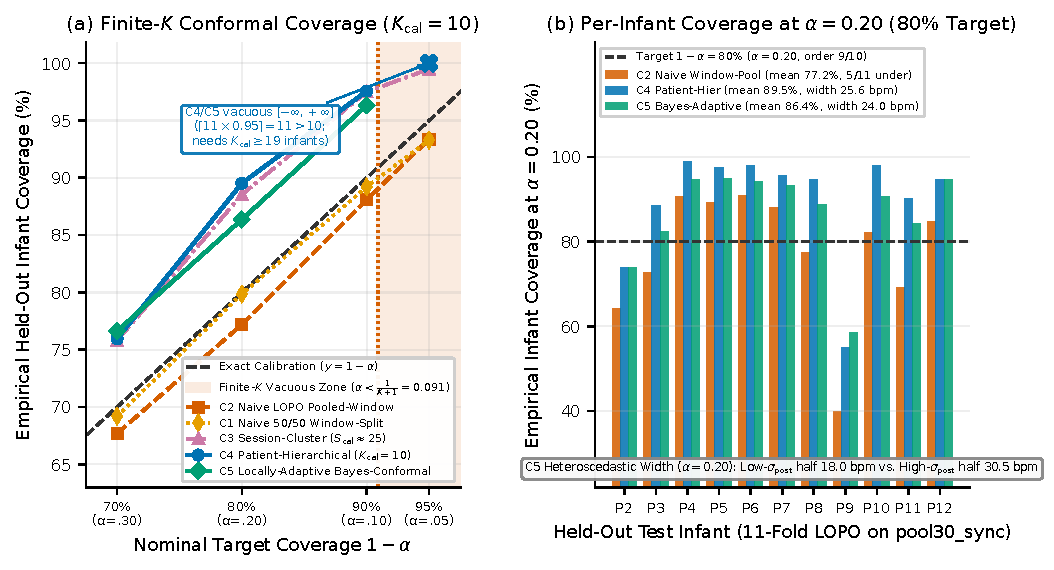
\includegraphics[width=0.95\textwidth]{stage3_finite_k_conformal_audit}
\caption{Frozen Stage~3 finite-$K$ conformal audit on R2e (1~Hz reference). Panel~(a) plots mean held-out infant coverage across nominal targets ($70\%$--$95\%$), marking the finite-$K$ vacuous zone ($\alpha < 1/(K_{\mathrm{cal}}+1)=0.091$) and vacuous 95\% C4/C5 intervals. Panel~(b) shows per-infant coverage across all 11 held-out infants at the 80\% target ($\alpha=0.20$) for C2, C4, and C5; in the embedded C5 callout, ``half'' denotes the within-patient median-split low-/high-$\sigma_{\mathrm{post}}$ window halves, and $18.0$/$30.5$~bpm are full interval widths, not half-widths.}
\label{fig:ch5_finite_k_conformal}
\end{figure}

\subsection{Head-to-head comparison with hierarchical methods}

The R2e 1~Hz head-to-head results are summarized in Table~\ref{tab:ch5_dunn_comparison}. At the 95\% target, the patient-level two-layer methods and the Dunn comparisons are all vacuous with ten calibration patients per fold. At the lower targets, CDF pooling generally has higher empirical patient coverage and larger intervals than the $B=200$ Monte Carlo single-draw subsampling average; C5 trades coverage against interval width differently. These are empirical comparisons across 11 held-out infants, not a universal ranking or a transfer of Dunn et al.'s guarantee to C4/C5.

\begin{table}[htbp]
\centering
\footnotesize
\setlength{\tabcolsep}{4pt}
\caption{R2e patient-level head-to-head conformal audit on the 1~Hz reference. Undercovered is the number of infants below target out of 11. Width is mean full interval width in bpm; bracketed values are within-patient median-split low-/high-posterior-SD full widths. The subsampling rows report the $B=200$ Monte Carlo average of single-draw subsampling. The 95\% row is vacuous for all listed methods; the 70\% block reports adaptive rows only (subgroup widths omitted).}
\label{tab:ch5_dunn_comparison}
\begin{tabularx}{\textwidth}{@{}c l >{\raggedright\arraybackslash}X r r@{}}
\toprule
Target & Form & Method & Mean / min cov; under & Mean width \\
\midrule
0.95 & All & C4, C5, Dunn CDF pooling, and single-draw subsampling ($B=200$ MC avg.) & 1.000 / 1.000; 0/11 & $\infty$ \\
\midrule
0.90 & Unweighted & C4 & 0.9756 / 0.8750; 1/11 & 38.84 \\
0.90 & Unweighted & Dunn CDF pooling & 0.9874 / 0.9144; 0/11 & 44.26 \\
0.90 & Unweighted & Dunn single-draw subsampling ($B=200$ MC avg.) & 0.9083 / 0.7020; 4/11 & 30.61 \\
0.90 & Adaptive & C5 & 0.9632 / 0.8472; 1/11 & 39.18 [29.30 / 49.82] \\
0.90 & Adaptive & Dunn CDF pooling & 0.9880 / 0.9213; 0/11 & 52.82 [39.51 / 67.17] \\
0.90 & Adaptive & Dunn single-draw subsampling ($B=200$ MC avg.) & 0.9056 / 0.7010; 4/11 & 33.83 [25.35 / 43.01] \\
\midrule
0.80 & Unweighted & C4 & 0.8952 / 0.5509; 2/11 & 25.57 \\
0.80 & Unweighted & Dunn CDF pooling & 0.8778 / 0.5926; 2/11 & 23.01 \\
0.80 & Unweighted & Dunn single-draw subsampling ($B=200$ MC avg.) & 0.8164 / 0.5003; 4/11 & 20.93 \\
0.80 & Adaptive & C5 & 0.8636 / 0.5856; 2/11 & 24.02 [17.96 / 30.54] \\
0.80 & Adaptive & Dunn CDF pooling & 0.8785 / 0.5903; 1/11 & 25.05 [18.74 / 31.86] \\
0.80 & Adaptive & Dunn single-draw subsampling ($B=200$ MC avg.) & 0.8174 / 0.5277; 4/11 & 22.64 [16.95 / 28.79] \\
\midrule
0.70 & Adaptive & C5 & 0.7661 / 0.4398; 3/11 & 17.62 \\
0.70 & Adaptive & Dunn CDF pooling & 0.7657 / 0.4213; 4/11 & 17.69 \\
0.70 & Adaptive & Dunn single-draw subsampling ($B=200$ MC avg.) & 0.7232 / 0.4010; 4/11 & 17.06 \\
\bottomrule
\end{tabularx}
\end{table}

\subsection{Audit of guarantee labels}

Structurally, C1 is unsuitable for a patient-level guarantee because random window splitting places windows from the same infant in calibration and evaluation. C2 uses patients for the outer split but still treats correlated pooled windows as exchangeable calibration units. C3 uses sessions that remain clustered within patient. Empirical mean coverage cannot repair a mismatch between the exchangeability unit and data structure.

{\sloppy The post-freeze adversarial audit found 146 conformal result entries across all stored cohorts, references, and models in \texttt{metrics\_stage3\_uncertainty.json} where \texttt{valid\_\allowbreak distribution\_\allowbreak free\_\allowbreak guarantee} was marked true for C2 or C3: eight for C2 and 138 for C3 (including 33 at vacuous $\alpha=0.05$). The flag logic depended on empirical mean coverage and did not establish a distribution-free guarantee. This field must not be used as evidence that either construction satisfies such a guarantee. C4 and C5 should likewise be described using their empirical LOPO coverage results; hierarchical assumptions and finite-$K$ rank restrictions remain explicit.\par}

\section{Interpretation and handoff}

Three conclusions follow from Stage~3. First, posterior standard deviation (U2) is the most defensible simple uncertainty score in this cohort: it is a direct posterior-spread measure without fitted parameters or an additional OOD barrier cutoff, and its selective-risk point estimates are favorable in both reference analyses. The patient-level gains do not survive Holm correction, so this is promising internal evidence rather than a confirmed improvement. Second, signal-quality rejection gives strong discrimination for the tested synthetic WGN condition, but its threshold controls a trade-off with quiet-apnea rejection. U6b at 0.90 met the project's two diagnostic limits in the tested cohort; it remains a fixed, empirically selected setting requiring broader evaluation. Third, ten calibration patients per LOPO fold make finite 95\% split-conformal intervals impossible under the stated rank rule. At lower targets, empirical coverage varies by patient, and the C4/C5 results do not establish nominal per-infant guarantees.

The Stage~3 clean-room audit passed all seven specified verification gates, including the Gate~G4 hard-freeze manifest check. The frozen Stage~4 model archive was recorded with SHA-256 \texttt{af33a83e\allowbreak 157f7d2e\allowbreak fb0f47e5\allowbreak 0c9544ee\allowbreak 19bacb7d\allowbreak a88ab0e0\allowbreak 235ccead\allowbreak 029cbcc4}. The subsequent Stage~4 benchmark evaluates the frozen models on an independent 24.2~GHz neonatal simulator without tuning on simulator data, providing controlled hardware-transfer evidence (Chapter~6). Because that benchmark uses a simulator rather than an independent patient cohort, it does not establish cross-site patient generalization or clinical performance. Exact reproduction of the original clinical cohort also remains unresolved because source identifiers and protocol details are incomplete. Further validation requires more independent calibration patients, externally collected infant data, prespecified pause-safety and OOD criteria, and prospective assessment of clinical utility.

\chapter{Zero-Touch External Hardware Transfer on a \texorpdfstring{\SI{24.2}{\giga\hertz}}{24.2 GHz} Neonatal Thorax Simulator}
\label{ch:external_transfer}

\section{Purpose and scope}

Chapter~5 examined selective uncertainty and finite-sample conformal calibration within the neonatal intensive-care-unit (NICU) reconstruction. This chapter asks a different question: do the frozen estimators retain their respiratory-rate tracking behavior when the radar hardware and signal source change? Stage~4 addresses this question with an independent 24.2~GHz radar recording of a controlled neonatal thorax simulator and a synchronized laser micrometer reference. The public dataset contains programmed sinusoidal breathing at ten rates from 5 to 80 breaths per minute (bpm), each in normal and deep excursion modes \citep{gleichauf2024time}.

This is a zero-touch hardware-transfer benchmark, not an external patient cohort. It tests whether models frozen after the NICU experiments can recover a known periodic mechanical signal on a different radar device, under a different acquisition chain, without external-data tuning. Its value is that the signal and reference are controlled and the hardware differs from the training system. Its limit is equally important: a simulator does not reproduce the variability, irregular breathing, motion, and clinical events found in infants. Results below support the bounded claim of transfer to these stationary simulator scenarios; they do not establish patient-level generalization, clinical accuracy, or bedside utility.

\section{External benchmark protocol}
\label{sec:ch6_protocol}

\subsection{Dataset, reference, and domain shift}

The external recordings are from the Gleichauf et al. neonatal thorax simulator dataset. A 24.2~GHz continuous-wave radar (InnoSenT iSYS-4001) records the simulated chest motion, while an approximately 2.5~kHz laser micrometer provides the independent displacement reference. The NICU system used in the earlier chapters operated at 24.0~GHz and 16~Hz. External radar I/Q data were acquired at approximately 2~kHz and deterministically decimated to the locked 16~Hz model input. Thus the transfer changes the radar unit and acquisition rate while retaining the frozen estimation pipeline and the independent physical reference.

The radar signal was mean-centered and passed through the locked zero-phase Kaiser FIR bandpass filter with $\firTaps=64$ taps, passband $[\bandLow,\bandHigh]=[0.30,3.00]$~Hz (18--180~bpm), and $\kaiserBeta=6.5$. The estimator's respiratory-rate grid is 18--90~bpm. Thus, 20~bpm lies within the grid but near the filter's lower transition skirt, whereas 5 and 10~bpm lie below both the passband and the estimator grid. The downsampling used two polyphase stages, first to approximately 200~Hz and then to 16~Hz; the resampling gain variation across the tested rates remained between $-0.0003$ and $+0.0023$~dB. The laser-derived steady-state rate was recomputed from the reference signal and used as the evaluation ground truth (matching the programmed rates within 0.036~bpm across all 20 scenarios). No model parameter, threshold, filter, window, scaler, or calibration quantile was adjusted using the external recordings.

The primary point estimate uses the full-cohort $K=11$ parameterization loaded from the frozen Stage~3 model archive. The archive's SHA-256 digest is \texttt{af33a83e\allowbreak 157f7d2e\allowbreak fb0f47e5\allowbreak 0c9544ee\allowbreak 19bacb7d\allowbreak a88ab0e0\allowbreak 235ccead\allowbreak 029cbcc4}. A leave-one-patient-out mean parameterization is reported as a sensitivity analysis; it was also transferred without external adaptation. The archive was frozen before this benchmark, and external data were used only for the one-shot evaluation.

\subsection{Scenario partition and evaluation window}

There are 20 programmed scenarios: rates of 5, 10, 20, 30, 40, 45, 50, 55, 60, and 80~bpm, each in normal and deep mode. For the Stage~4 report, scenarios were partitioned before scoring into an in-band set at or above 28~bpm and a sub-band set below 28~bpm. The resulting 14+6 partition is exhaustive (Table~\ref{tab:ch6_scenario_partition}). The 28~bpm boundary separates the primary operating region from the lower-frequency transition skirt and stopband; it is an operational reporting boundary, not a tested rate, since the nearest programmed conditions are 20 and 30~bpm. The analysis plan stated qualitative transfer goals, while the numeric thresholds in Gate~G5 are audit operationalizations rather than clinical decision thresholds.

\begin{table}[htbp]
\centering
\footnotesize
\caption{Exhaustive Stage~4 scenario partition. Each programmed rate was recorded in normal and deep excursion modes.}
\label{tab:ch6_scenario_partition}
\begin{tabularx}{\textwidth}{@{}>{\raggedright\arraybackslash}p{4.6cm}>{\raggedright\arraybackslash}Xr@{}}
\toprule
Stratum & Programmed rates & Scenarios \\
\midrule
In-band ($\brRef\geq28$~bpm) & 30, 40, 45, 50, 55, 60, 80~bpm & 14 \\
20~bpm FIR transition skirt & 20~bpm & 2 \\
05--10~bpm below-grid stopband & 5, 10~bpm & 4 \\
Sub-band total ($\brRef<28$~bpm) & 5, 10, 20~bpm & 6 \\
All scenarios & 5--80~bpm, ten programmed rates & 20 \\
\bottomrule
\end{tabularx}
\end{table}

The primary tracking metrics use overlapping 30~s windows advanced in 2~s steps, matching the prior stages, and retain steady-state windows only. Windows beginning before 10~s or ending within 10~s of the recording end were excluded, removing start and end synchronization steps. A separate all-window tracking sensitivity regime includes those transients, whereas the Stage~4 uncertainty risk--coverage audit evaluates steady-state windows and isolates the excluded start/end transients in a dedicated transient-detection check. In-band performance is summarized both as a scenario-macro mean, which weights the 14 conditions equally, and as a pooled-window metric. These summaries answer different questions and are not interchangeable. In total, the primary in-band evaluation contains 6,049 windows; the 5--10~bpm stopband comparison contains 1,731 windows.

\section{Zero-touch respiratory-rate transfer}
\label{sec:ch6_tracking}

\subsection{In-band accuracy and model complexity}

Within the 14 in-band conditions, the physics-constrained R0--R2 models track the simulator's stable periodic motion with very low scenario-macro error (Table~\ref{tab:ch6_model_transfer}). The primary frozen model, R2e, has a scenario-macro RMSE of 0.0197~bpm and a pooled-window $\rmsePool$ of 0.0262~bpm; its scenario-macro MAE is 0.0184~bpm. It achieves $\accTau{3}=\accTau{6}=\accTau{10}=100\%$, a calibration slope of 0.9994, and Pearson correlation $r=0.999999$ across scenario means. No steady-state R2e estimate differs from the laser reference by more than 0.5~bpm; its largest absolute error is 0.158~bpm. The LOPO-mean sensitivity gives a scenario-macro RMSE of 0.023~bpm, close to the full-cohort result.

R2e is the designated primary model because it is the frozen eight-parameter causal estimator carried forward from Stage~3, not because it wins every simulator point estimate. The 11-parameter R2a has a slightly lower scenario-macro RMSE (0.0189~bpm), and the offline R1f smoother is lower still (0.015~bpm) but is not a real-time comparator. R0 and the three-parameter causal R1a are also around 0.03~bpm. On this controlled in-band signal, adding parameters within the constrained family produces only tiny absolute differences.

\begin{table}[htbp]
\centering
\footnotesize
\setlength{\tabcolsep}{4pt}
\caption{Stage~4 steady-state tracking by model on the 14 in-band scenarios. RMSE, MAE, and bias are scenario-macro means in bpm; the 80~bpm and 20~bpm columns give RMSE for those two-scenario strata. R1f is an offline reference.}
\label{tab:ch6_model_transfer}
\begin{tabularx}{\textwidth}{@{}>{\raggedright\arraybackslash}Xrrrrrr@{}}
\toprule
Model & Params & RMSE & MAE & Bias & 80~bpm & 20~bpm \\
\midrule
R0 physical baseline & 0 & 0.028 & 0.027 & $-0.005$ & 0.063 & 0.069 \\
R1a causal forward estimator & 3 & 0.030 & 0.028 & $-0.007$ & 0.011 & 0.161 \\
R1f offline smoother & 3 & 0.015 & 0.014 & $+0.001$ & 0.010 & 0.053 \\
R2e causal, primary & 8 & 0.020 & 0.018 & $+0.001$ & 0.009 & 0.095 \\
R2a causal, 11-parameter & 11 & 0.019 & 0.017 & $+0.003$ & 0.020 & 0.024 \\
R3c spectral ridge & 439 & 3.635 & 3.607 & $+0.618$ & 10.465 & 11.778 \\
R3b spectral MLP & 14.6k & 3.502 & 3.447 & $+3.402$ & 1.065 & 32.704 \\
R3a causal TCN & 15.8k & 3.178 & 3.127 & $+0.695$ & 7.533 & 23.471 \\
\bottomrule
\end{tabularx}
\end{table}

The unconstrained rung-3 models show a different pattern. Their in-band scenario RMSEs range from 3.18 to 3.64~bpm, despite high scenario-level Pearson correlations (0.967--0.991). Correlation alone therefore hides errors in calibration and rate-dependent tracking: R3c has slope 0.709 and underestimates the 80~bpm condition, while R3b has a +3.402~bpm mean bias. Training sizes also differ: R3c and the R2 models were fit using all 11 NICU infants; R3a and R3b used 10, with one infant held out for early-stopping selection. This disclosure matters when interpreting the comparison, although all models were evaluated on the same independent simulator scenarios.

These findings support a limited inference: on the stable in-band simulator waveforms, the constrained signal-processing and state-space estimators transfer more reliably than the tested learned shortcuts. They do not show that a given model is more accurate on infants, where the reference modality, noise profile, and physiological variability differ from this controlled comparison.

\subsection{Rate-by-rate behavior and the filter boundary}

Table~\ref{tab:ch6_rate_by_rate} reports R2e for all 20 conditions, and Figure~\ref{fig:ch6_frequency_transfer} compares rate transfer and passband error across model rungs. Each cell gives scenario RMSE followed by the mean estimated rate in parentheses. From 30 through 80~bpm, the model follows the laser reference closely in both excursion modes. At 20~bpm, the fundamental lies near the lower FIR transition skirt: the fundamental is attenuated by approximately 10~dB, while its 40~bpm second harmonic remains in the passband. R2e remains close to the 20~bpm fundamental in both modes. The learned R3 models instead move toward their NICU training-rate distribution; their 20~bpm errors range from 11.78 to 32.70~bpm.

At 5 and 10~bpm, the signal is below the locked model grid and in the hardware stopband. R2e's reported mean estimates move toward higher apparent frequencies (about 40--50~bpm), consistent with tracking higher mechanical harmonics after rejection of the fundamental. This failure is a boundary of the 24~GHz CW and locked-filter setup, not evidence that the estimator can recover arbitrarily slow breathing. The sub-band is therefore reported as a diagnostic stress test, not included in the primary in-band accuracy claim.

\begin{table}[htbp]
\centering
\footnotesize
\setlength{\tabcolsep}{4.5pt}
\caption{Primary R2e results for every Stage~4 rate and excursion mode. Each mode entry is RMSE (mean estimated rate), in bpm; the laser column is the measured steady-state rate.}
\label{tab:ch6_rate_by_rate}
\begin{tabularx}{\textwidth}{@{}r>{\raggedright\arraybackslash}p{2.2cm}>{\raggedright\arraybackslash}Xrr@{}}
\toprule
Programmed rate & Laser $\brRef$ & Stratum & Normal RMSE (mean) & Deep RMSE (mean) \\
\midrule
5  & 4.98  & Stopband & 44.68 (49.3) & 42.89 (47.4) \\
10 & 10.02 & Stopband & 40.51 (49.9) & 31.28 (40.2) \\
20 & 19.98 & FIR skirt & 0.10 (20.1) & 0.09 (20.1) \\
30 & 30.00 & In-band & 0.04 (30.0) & 0.07 (30.1) \\
40 & 40.01 & In-band & 0.01 (40.0) & 0.02 (40.0) \\
45 & 44.99 & In-band & 0.00 (45.0) & 0.03 (45.0) \\
50 & 49.97 & In-band & 0.01 (50.0) & 0.02 (50.0) \\
55 & 55.01 & In-band & 0.01 (55.0) & 0.02 (55.0) \\
60 & 59.99 & In-band & 0.00 (60.0) & 0.03 (60.0) \\
80 & 79.96 & In-band & 0.01 (80.0) & 0.01 (80.0) \\
\bottomrule
\end{tabularx}
\end{table}

\begin{figure}[htbp]
\centering
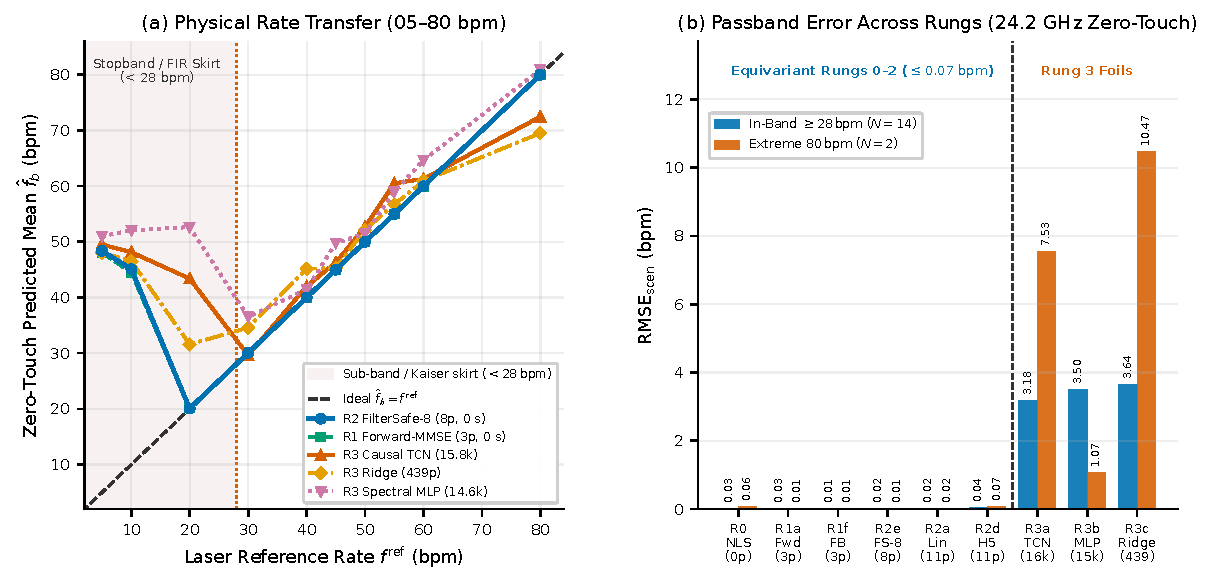
\includegraphics[width=0.95\textwidth]{stage4_external_frequency_transfer}
\caption{Zero-touch frequency transfer across the ten programmed rates and normal/deep simulator modes. Panel~(a) shows mode-averaged mean predicted rate against the laser reference relative to the locked 28~bpm reporting boundary, which separates the primary in-band results from the FIR transition skirt and below-grid stopband. Panel~(b) compares scenario-macro RMSE across Rungs~0--3 (including the R2d H5 variant) over the 14 in-band scenarios and the two 80~bpm scenarios.}
\label{fig:ch6_frequency_transfer}
\end{figure}

\section{Uncertainty and selective transfer}
\label{sec:ch6_uncertainty}

The external benchmark also tests whether Stage~3 uncertainty scores respond to simulator stopband signals and synchronization transients (Table~\ref{tab:ch6_uncertainty_transfer}). U6b retains the fixed $\tau_{\mathrm{ood}}=0.90$ cutoff and three-hop history selected in Stage~3; neither was retuned on the simulator. The stopband comparison uses steady-state windows and labels the four 5--10~bpm scenarios as out of distribution and the 14 in-band scenarios as in distribution. A separate broader comparison contrasts all six sub-band scenarios with the in-band set. These targets are deliberately distinct: success at identifying the 5--10~bpm stopband should not be read as reliable rejection across every frequency below 28~bpm.

\begin{table}[htbp]
\centering
\footnotesize
\setlength{\tabcolsep}{4pt}
\caption{Stage~4 uncertainty transfer for R2e. Risk is pooled RMSE across steady-state windows from all 20 scenarios (8,644 windows, excluding synchronization transients) at full and 80\% retention, in bpm. Stopband AUROC compares 1,731 steady-state windows at 5--10~bpm with 6,049 steady-state in-band windows; broad sub-band AUROC includes 20~bpm. Sync AUROC contrasts the 140 excluded start/end transient windows against the 6,049 steady-state in-band windows. All stopband FPR values were 0.000 at 95\% TPR.}
\label{tab:ch6_uncertainty_transfer}
\begin{tabularx}{\textwidth}{@{}>{\raggedright\arraybackslash}Xrrrr@{}}
\toprule
Proxy & RMSE ($1.0 \rightarrow 0.8$) & Stopband AUROC & Sub-band AUROC & Sync AUROC \\
\midrule
U1 posterior entropy & $17.973 \rightarrow 1.548$ & 0.9988 & 0.6679 & 0.7421 \\
U2 posterior SD & $17.973 \rightarrow 1.006$ & 0.9995 & 0.6685 & 0.7432 \\
U3 clean spectral entropy & $17.973 \rightarrow 1.014$ & 1.0000 & 0.9982 & 0.7459 \\
U4 raw spectral entropy & $17.973 \rightarrow 0.345$ & 1.0000 & 0.7484 & 0.7494 \\
U5 harmonic deficit & $17.973 \rightarrow 1.001$ & 1.0000 & 0.8552 & 0.4069 \\
U6a additive SQI & $17.973 \rightarrow 0.893$ & 1.0000 & 0.6687 & 0.7423 \\
U6b geometric SQI & $17.973 \rightarrow 0.893$ & 0.9998 & 0.6686 & 0.7422 \\
\bottomrule
\end{tabularx}
\end{table}

U6b separates the 5--10~bpm stopband from in-band simulator signals with AUROC 0.9998 and zero observed false positives at 95\% TPR; mean uncertainty is 0.0683 in-band and 0.2615 in the stopband. U2 also separates this specific stopband well (AUROC 0.9995). But discrimination falls to 0.6686 for U6b when the 20~bpm skirt is added to the out-of-band class. The composite is thus strong for the tested stopband and weak for the broader sub-band definition. It must not be described as a general frequency-boundary detector. The sync-transient AUROC is about 0.74, indicating only modest separation of those edge events.

Across steady-state windows from all 20 scenarios (8,644 windows, including stopband failures but excluding synchronization transients), the full-coverage pooled RMSE is 17.973~bpm. At 80\% retention, pooled RMSE spans 0.345~bpm for U4 to 1.548~bpm for U1, with U6a and U6b at 0.893~bpm and U2 at 1.006~bpm. This selective reduction is a descriptive result on the controlled mixture of in-band cases, stopband failures, and transients. It does not establish that a similar abstention rule would improve clinical monitoring, and the lowest-risk proxy here is not automatically appropriate for quiet-apnea handling in patient data. Figure~\ref{fig:ch6_uncertainty_conformal} summarizes this transfer and the interval results below.

\section{Conformal interval transfer}
\label{sec:ch6_conformal}

The frozen patient-calibrated C4 and C5 quantiles were applied to the primary R2e model without recalibration on simulator data. Stage~4 conformal results are reported only for R2e. The pre-freeze and post-freeze adversarial audits found that stored transfer quantiles for R1a and R2a reused the R2e quantile rather than each model's own; those fields are therefore excluded here. The full-cohort quantile uses 11 patient calibration units. At a 95\% target, its rank is $\lceil(11+1)0.95\rceil=12$, greater than the 11 available units, so the interval is vacuous; the finite-sample logic is developed in Chapter~5. The finite targets shown below are 90, 80, and 70\%.

Table~\ref{tab:ch6_conformal_transfer} reports mean full interval width, not a half-width or a value to be doubled. Coverage is summarized across simulator scenarios as the mean and minimum scenario coverage. For the 14 in-band conditions, both C4 and C5 cover every evaluated window at all three targets. The 13.27--39.08~bpm in-band widths are nevertheless broad relative to the approximately 0.02~bpm in-band RMSE; perfect observed coverage here is not evidence of a useful clinical interval or a distribution-free guarantee.

\begin{table}[htbp]
\centering
\footnotesize
\setlength{\tabcolsep}{4.5pt}
\caption{Zero-touch external conformal transfer for the frozen R2e model. Width is mean full interval width in bpm; coverage is scenario mean / minimum. The quantiles were calibrated on NICU data and not adjusted on the simulator.}
\label{tab:ch6_conformal_transfer}
\begin{tabularx}{\textwidth}{@{}>{\raggedright\arraybackslash}Xcrrrr@{}}
\toprule
Stratum & Target & C4 width & C4 coverage & C5 width & C5 coverage \\
\midrule
In-band & 90\% & 39.08 & 1.000 / 1.000 & 29.34 & 1.000 / 1.000 \\
In-band & 80\% & 26.86 & 1.000 / 1.000 & 18.02 & 1.000 / 1.000 \\
In-band & 70\% & 16.56 & 1.000 / 1.000 & 13.27 & 1.000 / 1.000 \\
\midrule
Sub-band & 90\% & 39.08 & 0.350 / 0.000 & 41.62 & 0.421 / 0.046 \\
Sub-band & 80\% & 26.86 & 0.338 / 0.000 & 25.57 & 0.360 / 0.016 \\
Sub-band & 70\% & 16.56 & 0.333 / 0.000 & 18.82 & 0.343 / 0.002 \\
\midrule
All 20 & 90\% & 39.08 & 0.805 / 0.000 & 33.03 & 0.826 / 0.046 \\
All 20 & 80\% & 26.86 & 0.801 / 0.000 & 20.29 & 0.808 / 0.016 \\
All 20 & 70\% & 16.56 & 0.800 / 0.000 & 14.93 & 0.803 / 0.002 \\
\bottomrule
\end{tabularx}
\end{table}

The high in-band coverage and low sub-band coverage reveal a strong domain boundary. At the 80\% target, C5's scenario-mean coverage is 1.000 in-band but 0.360 in the sub-band; its minimum sub-band scenario coverage is 0.016. Across all 20 scenarios, C5 reaches a scenario-mean (and pooled) coverage of 0.808, but its worst-scenario minimum is 0.016. C4 is also highly undercovered outside the in-band region. The apparently acceptable all-scenario average therefore conceals conditions in which the transferred intervals miss nearly every window. Coverage over repeated windows from a small set of simulator scenarios is descriptive and does not create independent patient-level calibration units.

\begin{figure}[htbp]
\centering
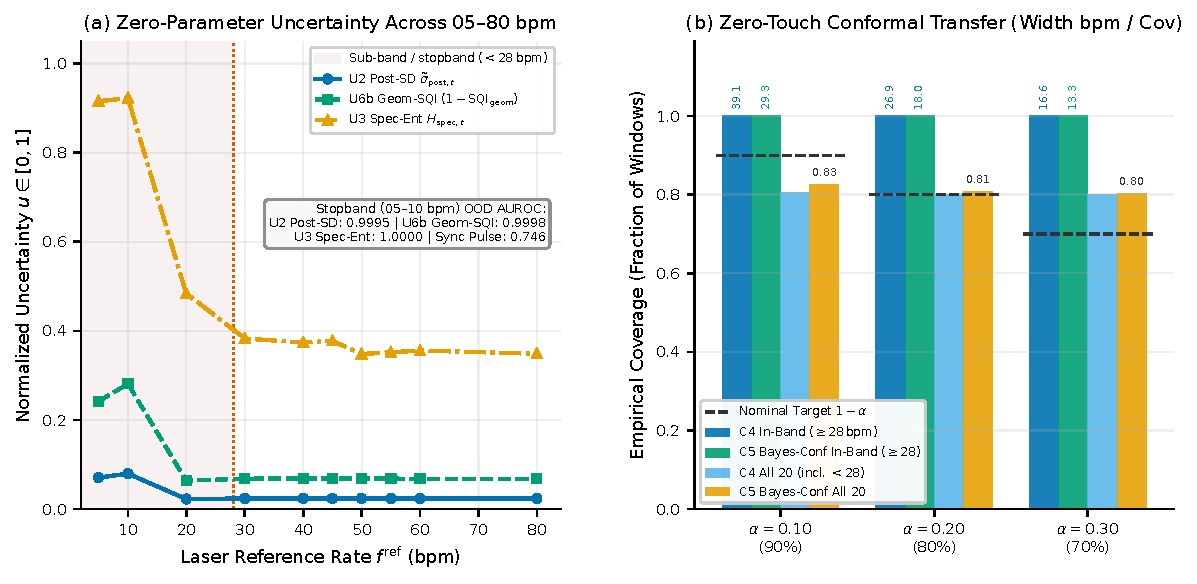
\includegraphics[width=0.95\textwidth]{stage4_external_uncertainty_and_conformal}
\caption{Stage~4 uncertainty and conformal transfer. Panel~(a) shows mode-averaged U2, U6b (zero fitted weights, locked $\tau_{\mathrm{ood}}=0.90$, and 3-hop history), and U3 scores across programmed rates, with the stopband discrimination inset and U3 synchronization-pulse AUROC (0.746). Panel~(b) compares C4 and C5 scenario-mean coverage across the 14 in-band scenarios ($\geq 28$~bpm) and all 20 scenarios, annotated with in-band mean full interval widths (sub-band breakdowns appear in Table~\ref{tab:ch6_conformal_transfer}).}
\label{fig:ch6_uncertainty_conformal}
\end{figure}

\section{Independent audit, interpretation, and limitations}

An independent clean-room audit passed all seven Stage~4 gates. It verified all 49 external source-file hashes, the disjoint 14+6 scenario partition, the laser-derived reference on independent sentinels, raw-to-16~Hz preprocessing and model outputs, stratified metrics, uncertainty and conformal results, and the serialized Gate~G5 contract. The audit confirmed the frozen archive digest given above. For the primary H0 pipeline, external $SO(2)\times\mathbb{R}_{>0}$ invariance deviations remained within $2.84\times10^{-14}$, with a quadrature-swap Nyquist residual within $2.58\times10^{-5}$~bpm; for the external H5 $O(2)\times\mathbb{R}_{>0}$ variant, the independent clean-room recomputation reported a maximum deviation of $1.42\times10^{-14}$. Sequence-level future-window perturbation tests produced exactly zero output difference for the evaluated causal sequence models and uncertainty filters (while primary H0-backed estimators still retain the fixed 3~s STFT/HPSS window lookahead). These are software and signal-processing verification results under the tested transformations, not evidence of robustness to every acquisition failure.

Taken together, Stage~4 supports three conclusions. First, the physics-constrained model family transfers with very small rate error across the simulator's in-band sinusoidal conditions, while the tested high-capacity learned models show larger calibration errors and fail at particular rate boundaries. Second, the frozen uncertainty scores identify the 5--10~bpm stopband well, but this result does not extend to the entire below-28~bpm region or to clinical artifact detection. Third, patient-derived intervals transfer empirically to the in-band simulator but under-cover substantially in the sub-band, especially at the scenario level. Each conclusion is bounded by the measured conditions and the frozen estimator pipeline.

The simulator provides controlled ground truth but only a restricted model of breathing. Its regular sinusoidal motion does not represent irregular respiratory cycles, pauses, apnea events, mixed motion, changing body position, or the noise and reference uncertainty of clinical care; the dataset authors likewise describe the simulator as covering basic functions rather than the full range of real breathing \citep{gleichauf2024time}. The study tests one external radar design at 24.2~GHz and one fixed signal-processing pipeline. Its very small in-band errors result from stable periodic signals and should not be read as expected error in an infant. The lower-frequency results show a practical limitation of the locked filter and single-channel CW measurement: below the modeled frequency range, the fundamental is attenuated or rejected and the estimate can follow a higher harmonic. The conformal results show that calibration on patient residuals does not guarantee transfer across this signal shift.

Gate~G5 therefore supports the thesis's L4 claim of zero-touch transfer to a controlled external hardware simulator. It does not authorize L5 claims of clinical superiority, bedside utility, autonomous apnea alarming, or safe use in an infant-monitoring workflow. Resolving those questions requires externally collected patient recordings, prospectively defined clinical and safety endpoints, broader hardware and site variation, and calibration cohorts large enough to support informative patient-level intervals. Chapter~7 discusses these limits and the next validation steps.

\chapter{Discussion, Clinical Readiness Gap, Limitations, and Conclusion}
\label{ch:discussion_conclusion}

This thesis examined contactless neonatal respiratory-rate estimation as a chain of
measurement, signal processing, inference, and decision-making. The results do not support a
single claim that a high-accuracy estimator is ready to replace a bedside monitor. They support a
more bounded conclusion: in the evaluated cohort, a compact model with explicit signal and
temporal structure was more robust than the tested unconstrained regressors; simple uncertainty
scores and a fixed quality barrier exposed useful failure information; and independent phantom
measurements demonstrated controlled hardware transfer. At the same time, differences between
the available respiratory references, patient-level interval widths, and the absence of a
prospective clinical evaluation leave bedside utility unresolved.

The distinction matters because the output of a radar pipeline is not determined by its estimator
alone. Synchronization changes which samples are compared. A monitor trend and a rate computed
from individual respiratory triggers encode different timing and pause conventions. Filtering
sets the range of rates the system can represent. Finally, selective rejection and interval
calibration determine what a user sees when the signal becomes ambiguous. The following
discussion interprets the thesis across these connected stages and states the resulting claim
boundary explicitly.

\section{What the results establish}
\label{sec:ch7_synthesis}

\subsection{The value and limits of physical inductive bias}

The point-estimation results favor a structured, low-capacity model over the specific
high-capacity regressors evaluated here. On the 11-infant, 28-session \texttt{pool30\_sync}
cohort, the eight-parameter causal differentiable HMM R2e reduced equal-session RMSE relative to
the memoryless R0 baseline by 0.9687~bpm on the 1~Hz monitor reference (95\% interval
[$-1.1347,-0.8034$]; patient-level Holm-adjusted $p=0.0117$) and by 0.6635~bpm on the shared
\texttt{Trig -10 s} reference ($[-0.8833,-0.4464]$; Holm-adjusted $p=0.0215$). The paired
improvement appeared in 11/11 infants on the monitor reference and 10/11 on the lag-adjusted
trigger reference. This is evidence for R2e over R0 within the frozen evaluation protocol; it is
not evidence that the radar estimates a clinically adjudicated respiratory rate without error.

The comparison with the three-parameter forward-MMSE model R1a is more restrained. R2e's
one-hertz point estimate was 0.1418~bpm lower, but the patient-level comparison was not
significant after multiplicity correction ($p_{\mathrm{pat}}=0.0830$;
$p_{\mathrm{pat,Holm}}=0.6641$). The patient-level comparison on \texttt{Trig -10 s} was also
non-significant ($p_{\mathrm{pat}}=0.5771$). Thus the evidence supports a useful gain over the
memoryless baseline, while the cohort does not resolve whether eight parameters improve on the
much smaller temporal model. This pattern is consistent with a practical saturation point: a
small amount of causal temporal structure appears valuable, but the additional complexity of
R2e has not been shown to yield a reliable patient-level gain over R1a.

The unconstrained R3 regressors illustrate why parameter count alone is not the relevant
comparison. Their apparent internal advantages varied by reference, and they showed variance
shrinkage and weaker performance on the trigger-based evaluation. On the independent Stage~4
phantom, their in-band scenario RMSEs were 3.18--3.64~bpm, while R2e's was 0.0197~bpm with a
calibration slope of 0.9994. R3a and R3b used ten training infants, with one infant reserved for
checkpoint selection; R3c and R2e used all eleven. The training difference is a fairness
limitation, although R3c also showed substantial phantom error. The results therefore support
physical and shift-equivariant constraints over these tested shortcuts in these evaluations, not
a general conclusion that neural models cannot transfer. Shortcut learning is a recognized risk
when models can exploit correlations that do not persist under shift \citep{geirhos2020shortcut}.

The independent lines of evidence are complementary rather than interchangeable. Stage~2 tests
patient-held-out estimation on NICU recordings; Stage~4 tests frozen algorithms on controlled
stationary phantom motion. The Stage~4 benchmark comprised twenty conditions, fourteen in the
filter's in-band range and six below it. R2e performed exceptionally on the stable in-band
phantom signals, but Stage~4 contained no infants, spontaneous motion, clinical care, or bedside
reference uncertainty. Its result supports the project's L4 claim of zero-touch physical
transfer under the tested protocol. It cannot be used as evidence of L5 clinical utility.

\subsection{Uncertainty is useful only when its operating limits are visible}

The uncertainty analyses do not establish a second, independently validated clinical benefit.
U2, posterior standard deviation, is attractive because it is a direct posterior-spread score
with no fitted parameters or additional cutoff. Its session-level E-AURC was
$-0.2454$~bpm (95\% interval [$-0.4069,-0.1168$]) on the monitor reference and
$-0.2929$~bpm ([$-0.4555,-0.1436$]) on the trigger reference. At 80\% retained coverage it
reduced the one-hertz session-macro RMSE from 6.8486 to 6.6890~bpm; 10/11 infants improved. The raw
patient-level $p$-value was 0.0098, but the Holm-adjusted value was 0.0781. On the trigger
reference, 9/11 infants improved and the raw $p$-value of 0.0244 became 0.1953 after Holm
correction. The negative E-AURC estimates and these patient-level patterns are promising
internal evidence, not multiplicity-adjusted confirmation that U2 improves clinical decisions.

U6b addresses a different operating need: it combines posterior and spectral information to
flag questionable signal windows while limiting rejection during quiet pause-like intervals.
Its weights are not fitted, but it uses the fixed, empirically informed
$\tau_{\mathrm{ood}}=0.90$ cutoff and a three-hop (6~s) history. At that setting the pause-rejection
ratio was 1.1275 pooled and 1.1209 session-macro, within the project's 1.15 criterion; the
synthetic white-noise AUROC was 0.9986, with a 0.0036 false-positive rate at 95\% sensitivity.
On Stage~4, U6b separated the tested 5--10~bpm stopband conditions from in-band phantom motion
with AUROC 0.9998. When the 20~bpm skirt was added to the out-of-band class, its AUROC fell to
0.6686. Accordingly, the evidence supports a useful but fixed heuristic for the tested pause
and corruption conditions. It does not establish a generally reliable OOD detector or a
threshold-free method.

The learned five-parameter U6c score provides a counterexample to treating selective-risk
performance as the only criterion: although its risk--coverage point estimates were favorable,
its pause-rejection ratio of 1.2266 exceeded the project's 1.15 limit. Conversely, U6b's safer
pause ratio does not make it universally superior. Score ranking, pause preservation, corruption
detection, and patient-level uncertainty are separate properties and should remain separately
reported. In this cohort, a safe monitor design would expose quality or uncertainty to the
operator without silently suppressing a potentially important pause.

\section{The gap between phantom transfer and clinical readiness}
\label{sec:ch7_readiness}

The clearest quantitative readiness gap is the difference between Stage~4 point accuracy and
Stage~3 patient-level uncertainty. R2e's 0.0197~bpm scenario-macro RMSE on the in-band phantom
reflects a stable periodic signal with a laser reference. In the clinical cohort, the locally
adaptive C5 interval procedure at an 80\% target had a mean full width of 24.02~bpm. Its mean
patient coverage was 0.864, but the minimum was 0.586 and two of eleven infants were below the
nominal target. The full width averaged 17.96~bpm in the lower-posterior-uncertainty group and
30.54~bpm in the higher-uncertainty group. These widths are cohort-specific empirical results;
they are not half-widths, and they do not establish a universal physical limit of 24~GHz radar.
They show that, for this model, front end, cohort, and calibration design, intervals wide enough
to cover patient-level errors can be poorly suited to narrow rate decisions.

The finite-sample rank constraint is more fundamental to the current 95\% calibration claim. In
each leave-one-patient-out fold, only ten infants are available for calibration. The patient-level
order-statistic rank at 95\% is
\[
  \left\lceil (K_{\mathrm{cal}}+1)(1-0.05)\right\rceil
  =\lceil 11\times0.95\rceil=11,
\]
which exceeds the ten observed calibration units. A finite patient-exchangeable 95\% interval
therefore cannot be returned by this rank construction; its set is vacuous. At least
$K_{\mathrm{cal}}=19$ independent calibration patients are required for a finite 95\% interval
under this rule. That is a mathematical minimum for rank resolution, not a sufficient sample
size for clinical validation, subgroup precision, or safe alarm evaluation. Repeated windows
from the same infant do not increase the number of independent calibration patients. This
distinction between window-level abundance and patient-level information is central to
interpreting conformal intervals in clustered clinical data \citep{dunn2023distribution,barber2023conformal}.

These interval results also need careful interpretation at the 80\% target. C5 is a two-level,
locally adaptive calibration procedure informed by hierarchical conformal methods. If the same
nominal level is used at both levels, the simple hierarchical coverage bound under the required
assumptions is $(1-\alpha)^2=0.64$, not 0.80; the present analysis does not establish those
assumptions or a distribution-free, per-infant 80\% guarantee \citep{dunn2023distribution}.
Its reported coverage is empirical and heterogeneous across infants. Wider calibration sets or
a different cohort could change both coverage and width. The 24.02~bpm mean full width is
therefore best treated as a readiness diagnostic for the present single-channel pipeline, not
as a sensor specification or immutable information-theoretic bound.

The NICU recordings also contain plausible sources of ambiguity that are not represented by a
stationary phantom. At the session level, the fraction of windows in the cardiac HR/2 collision
band was associated with excess respiratory-rate error (Spearman $\rho=+0.696$,
$p<10^{-4}$). This association is consistent with harmonic ambiguity but does not prove that
cardiac motion caused the error. Session~11.1 had an I/Q standard-deviation ratio of 5.86,
absolute I/Q correlation of 0.863, and clipping in 5.06\% of samples; its shared-lag RMSE was
12.65~bpm. Session~9.2 also contained intervals where the recorded UCD status was not
\texttt{ChildPresent}. Random body movement and receiver or firmware interruptions add further
variation. These examples document observed failure contexts; they do not provide a causal
decomposition of the whole cohort.

The target reference itself is a limitation. The 1~Hz monitor stream and the trigger-derived
rates do not measure exactly the same quantity. One comparison excludes inter-trigger gaps over
five seconds, while a whole-window count includes the pause duration; these pause-like windows
are not clinically adjudicated apnea diagnoses. Differences between references, monitor delay,
and synchronization can all affect measured error. A prospective evaluation will need a
prespecified reference protocol, explicit timing alignment, and a clear treatment of pauses,
missingness, and alarm events. Neither the present internal references nor the stationary
phantom can show that a radar alarm would improve outcomes or safely replace a wired monitor.

Label-dependent online conformal adaptation does not remove this gap by itself. In standard
adaptive conformal inference, the update uses the realized miss indicator
$e_t=\mathbb{1}\{y_t\notin\widehat{C}_t(\alpha_t)\}$ to modify the next miscoverage level, for example
\[
  \alpha_{t+1}=\alpha_t+\gamma(\alpha-e_t).
\]
The indicator cannot be computed until a reference respiratory rate is observed. If a bedside
system has no concurrent reference label, this feedback update is unavailable; it cannot
autonomously adapt its interval from the radar stream alone. ACI and related online methods remain
possible in a supervised shadow study, or with delayed and independently measured labels, but
their label requirement and operational delay must be part of the design \citep{gibbs2024conformal,angelopoulos2024conformal}.

\section{Limitations and claim boundaries}
\label{sec:ch7_limitations}

Several limitations qualify the conclusions. First, the internal cohort contains eleven infants
and 28 synchronized sessions. The infant, rather than the one-hertz window, is the relevant
independent unit for claims about performance across patients. This sample constrains power for
close model comparisons, subgroup analysis, and patient-level conformal calibration. In
particular, failure to detect an R2e--R1a difference is not proof of equivalence.

Second, the references are imperfect and operationally distinct. The monitor trend has temporal
smoothing and delay; respiratory-trigger rates depend on trigger timing and on whether long gaps
are omitted from the rate denominator. The chapter results consequently answer a comparison
question under defined reference constructions, not an absolute measurement-accuracy question
against a universally valid gold standard. Patient-level analyses reduce the risk of treating
correlated windows as independent evidence, but they cannot resolve uncertainty in the reference
labels themselves.

Third, the acquisition and front-end choices bound the observable rate range. The locked
64-tap zero-phase Kaiser FIR passband is 0.30--3.00~Hz. The 5--10~bpm phantom conditions lie
below its lower edge, and rates in that region cannot be inferred reliably from the current
filtered representation. Raising the low-frequency response or changing the window and
separation stages could extend the range, but those changes would alter the frozen pipeline and
require new tests of latency, motion artifacts, harmonic confusion, and patient-level safety.
The present work does not validate severe bradypnea detection.

Fourth, some uncertainty design choices remain empirical. U6b's fixed cutoff of 0.90 and
three-hop history satisfy the selected pause and white-noise criteria on this cohort, while
nearby choices reveal a trade-off. The HQI harmonic-deficit normalization also compresses its
observed range and is highly correlated with an alternative non-overlapping denominator
(Spearman $\rho=0.999945$); this is a reason to interpret its scale cautiously, even though the
ranking is similar. These engineering decisions should be frozen before external clinical
testing and assessed across receiver settings and care conditions.

Fifth, Stage~4 is deliberately narrow. It tests stationary sinusoidal phantom movement on
independent 24.2~GHz hardware and supports a zero-touch L4 transfer result for the tested
protocol. The performance does not establish transfer to infants, across institutions, or to
different radar placements and waveforms. Exact reproduction of the original Beltr\~ao et al.
clinical subset also remains unresolved because cohort identifiers, the precise denominator,
and parts of the synchronization and solver protocol are unavailable. The work therefore does
not claim exact reproduction of that study (L2), nor clinical bedside utility, autonomous apnea
alarming, or superiority to wired NICU monitoring (L5) \citep{beltrao2022contactless}.

These boundaries are consistent with broader reviews of neonatal non-contact and wireless
monitoring, which report small studies, limited evaluation of feasibility and safety, and
methodological gaps alongside technical promise \citep{senechal2026next}. Such context does not
validate or invalidate the present estimator; it reinforces the need to evaluate signal
availability, safety, reference quality, and workflow in addition to point accuracy.

\section{Next research steps}
\label{sec:ch7_future}

The next phase should address both sensing ambiguity and the lack of independent patient-level
evidence. On the engineering side, multi-antenna or wideband FMCW measurements could provide
range and spatial information that a single-channel CW system does not observe. Range-bin
isolation may help distinguish thoracic motion from other moving reflectors, while optical or
time-of-flight channels could provide complementary motion information. These are research
directions, not guaranteed fixes: additional channels introduce calibration, synchronization,
privacy, and device-integration requirements. Recent neonatal radar and multimodal studies
provide relevant starting points for controlled comparisons \citep{liao2025noncontact,hari2025contactless,gleichauf2021automated}.

The statistical work should first expand the number of independent infants. Nineteen calibration
patients is the rank-based minimum for a finite patient-level 95\% interval under the stated
order-statistic rule; a larger multicenter cohort will be needed to estimate performance across
gestational ages, body sizes, clinical support, motion states, and sites. The final sample size
should follow a prespecified precision or power calculation and account for unusable recordings
and site-level variation. Calibration and evaluation must be separated at the patient and,
where appropriate, site level. Any proposed conformal procedure should be audited for its actual
exchangeability unit, finite-sample rank, coverage by patient and subgroup, interval width, and
behavior under distribution shift rather than relying on a stored validity flag alone.

Clinical testing should proceed prospectively in shadow mode while existing monitoring remains
available. The protocol should define the intended use before data collection: respiratory-rate
trend display, quality warning, or candidate alarm support are different functions and require
different endpoints. It should measure usable-data availability, time alignment, error and
coverage by infant, false and missed alarms, alert delay, pause handling, and the burden of
non-actionable alerts. Any transition toward interventional use would require ethics review,
appropriate parent or guardian consent, privacy and data-governance protections, and a clear
clinical oversight and escalation pathway. The safety case must make abstention visible and must
not turn a rejected radar window into silence when the underlying event could be clinically
important.

\section{Ethics, reproducibility, and conclusion}
\label{sec:ch7_ethics_conclusion}

The principal ethical constraint is to avoid presenting a research estimate as a replacement for
clinical observation. In particular, a quality filter that rejects a pause-like window can hide
the very period that requires review. Future interfaces should distinguish a low-confidence
estimate from a low respiratory rate, preserve access to the underlying signal and quality
status, and defer clinical action to an approved workflow. Data use, access, storage, and any
future model update must follow the applicable institutional and clinical governance. The use
of Paper Orchestra and other AI-assisted drafting or editorial tools should be disclosed
in the required authorship declaration, including the tools and scope of assistance and the
distinction between editorial support and scientific analysis. Responsibility for the scientific
claims, analyses, and final text remains with the author.

The project records a frozen analysis basis at commit \texttt{5e458c1}, with the legacy baseline
environment identified as Python~3.9.6 and the WP1--WP5 research pipeline as Python~3.10.19.
The reproducibility appendix reports integrity checks for the archived scripts, caches,
figures, bibliography, and notation contract. Those records support review of how the reported
results were produced; they do not substitute for independent replication or release of data
that cannot ethically or legally be shared.

In conclusion, this thesis finds that a compact, physics-constrained causal estimator can
outperform a memoryless baseline across two defined NICU references and can transfer with very
low error to an independent stationary phantom. It also shows that posterior uncertainty and a
carefully selected quality barrier can help characterize when estimates may be unreliable, while
finite patient counts impose sharp limits on interval resolution. The evidence is strongest for
the value of explicit structure and disciplined evaluation within the tested system. It remains
insufficient for a claim of prospective bedside utility. The responsible next step is larger,
patient-level, multicenter validation with transparent uncertainty, preserved standard care, and
predefined safety outcomes.


% --- BIBLIOGRAPHY ---
\cleardoublepage
\bibliographystyle{unsrtnat}
\bibliography{../paper_orchestra_bundle/raw_materials/seed_references}

% --- APPENDICES ---
\appendix
\chapter{Master Notation Glossary and Code-to-Manuscript Contract}
\label{app:notation}

{\sloppy
The authoritative notation table below is loaded verbatim from the immutable contract file
\texttt{paper\_\allowbreak orchestra\_\allowbreak bundle/\allowbreak raw\_\allowbreak materials/\allowbreak notation\_\allowbreak glossary.tex}
(sealed under commit \FrozenGitCommit{}) and rendered here under A4~\SI{16.0}{\centi\meter}
geometry without altering its byte contents.
\par}

\begingroup
\singlespacing
\scriptsize
\emergencystretch=1.8em
\let\NOTATIONMACROSONLY\undefined
% =============================================================================
% notation_glossary.tex
% Single Authoritative Symbol, Macro, Python Identifier & Figure-Label Lock
% Project : Non-Contact NICU Radar Breathing Monitoring (Master's Thesis)
% Authors : Frozen across Python docstrings (paper_workspace/src/*.py),
%           PaperOrchestra (google-research/paper-orchestra) dense inputs,
%           Matplotlib/TikZ figures, and LaTeX thesis chapters.
%
% USAGE:
%   1. In thesis main.tex PREAMBLE (loads macros only):
%        \def\NOTATIONMACROSONLY{1}
%        % =============================================================================
% notation_glossary.tex
% Single Authoritative Symbol, Macro, Python Identifier & Figure-Label Lock
% Project : Non-Contact NICU Radar Breathing Monitoring (Master's Thesis)
% Authors : Frozen across Python docstrings (paper_workspace/src/*.py),
%           PaperOrchestra (google-research/paper-orchestra) dense inputs,
%           Matplotlib/TikZ figures, and LaTeX thesis chapters.
%
% USAGE:
%   1. In thesis main.tex PREAMBLE (loads macros only):
%        \def\NOTATIONMACROSONLY{1}
%        \input{paper_orchestra_bundle/raw_materials/notation_glossary.tex}
%   2. In thesis Appendix / Nomenclature chapter BODY (prints full tables):
%        \let\NOTATIONMACROSONLY\undefined
%        \input{paper_orchestra_bundle/raw_materials/notation_glossary.tex}
%   3. Requires standard LaTeX packages in parent document:
%        amsmath, amssymb, booktabs, longtable, array
% =============================================================================

% -----------------------------------------------------------------------------
% PART A: CANONICAL SEMANTIC LATEX MACROS (\providecommand avoids collisions)
% -----------------------------------------------------------------------------

% --- Physical & Radar Front-End Parameters (WP1) ---
\providecommand{\speedLight}{c}
\providecommand{\carrierFreq}{f_c}
\providecommand{\radarLambda}{\lambda}
\providecommand{\fsRadar}{f_s}
\providecommand{\fsRefRaw}{f_{s,\mathrm{ref}}}
\providecommand{\fsRefRate}{f_{s,\mathrm{rate}}}
\providecommand{\nomRange}{d_0}
\providecommand{\chestDisp}{d(t)}
\providecommand{\chestDispResp}{d_{\mathrm{resp}}(t)}
\providecommand{\chestDispCard}{d_{\mathrm{card}}(t)}
\providecommand{\chestDispRBM}{d_{\mathrm{RBM}}(t)}
\providecommand{\chestDispEst}{\hat{d}(t)}
\providecommand{\phaseSig}{\phi(t)}
\providecommand{\phaseZero}{\theta_0}
\providecommand{\modIndex}{\beta_{\mathrm{mod}}}
\providecommand{\besselJ}[2]{J_{#1}\!\left(#2\right)}
\providecommand{\iqI}{b_I(t)}
\providecommand{\iqQ}{b_Q(t)}
\providecommand{\iqComplex}{z(t)}
\providecommand{\iqGainImb}{g}
\providecommand{\iqPhaseSkew}{\psi}
\providecommand{\iqDcI}{c_I}
\providecommand{\iqDcQ}{c_Q}
\providecommand{\csdSignal}{x(t)}
\providecommand{\csdClean}{\hat{x}(t)}
\providecommand{\adPhase}{\hat{\phi}_{\mathrm{AD}}(t)}
\providecommand{\dacmPhase}{\hat{\phi}_{\mathrm{DACM}}(t)}

% --- Filtering, Windowing & STFT Decomposition (WP2) ---
\providecommand{\winSec}{W}
\providecommand{\updateSec}{\Delta_{\mathrm{upd}}}
\providecommand{\winSamples}{N_w}
\providecommand{\bandLow}{f_{\mathrm{low}}}
\providecommand{\bandHigh}{f_{\mathrm{high}}}
\providecommand{\firTaps}{M_{\mathrm{FIR}}}
\providecommand{\kaiserBeta}{\beta_{\mathrm{K}}}
\providecommand{\stftWin}{N_{\mathrm{win}}}
\providecommand{\stftHop}{H_{\mathrm{stft}}}
\providecommand{\stftNfft}{N_{\mathrm{FFT}}}
\providecommand{\stftComplex}{X[k,m]}
\providecommand{\stftMag}{\lvert X[k,m] \rvert}
\providecommand{\stftPhase}{\angle X[k,m]}
\providecommand{\stftMagFilt}{\lvert \hat{X}[k,m] \rvert}

% --- NMF/RBM Baseline vs HPSS Variants (WP2) ---
\providecommand{\nmfRank}{K_{\mathrm{NMF}}}
\providecommand{\nmfW}{\mathbf{W}}
\providecommand{\nmfH}{\mathbf{H}}
\providecommand{\hoyerSpar}{\sigma_{\mathrm{Hoyer}}}
\providecommand{\rbmAlpha}{\alpha_{\mathrm{RBM}}}
\providecommand{\rbmSparThresh}{\tau_{\mathrm{Hoyer}}}
\providecommand{\nRemoved}{n_{\mathrm{rem}}}
\providecommand{\hpssHarm}{S_H}
\providecommand{\hpssPerc}{S_P}
\providecommand{\hpssMask}{M_H}
\providecommand{\hpssMaskBand}{M_{H,\mathrm{band}}}
\providecommand{\hpssLenH}{L_H}
\providecommand{\hpssLenP}{L_P}
\providecommand{\hpssGamma}{\gamma}
\providecommand{\hpssEps}{\varepsilon}
\providecommand{\hpssMargin}{\beta_{\mathrm{sep}}}
\providecommand{\hpssKeptFrac}{\kappa_{\mathrm{kept}}}

% --- Harmonic NLS, HQI & Viterbi State-Space Tracking (WP3) ---
\providecommand{\psdFolded}{P(f)}
\providecommand{\autocorrFn}{r_{\mathrm{ac}}[\tau]}
\providecommand{\freqCoarse}{\hat{f}_{\mathrm{coarse}}}
\providecommand{\nlsOrder}{L_k}
\providecommand{\nlsRadius}{\Delta_{\mathrm{NLS}}}
\providecommand{\nlsStep}{\delta_{\mathrm{NLS}}}
\providecommand{\nlsCost}{\mathcal{J}_{\mathrm{NLS}}(f)}
\providecommand{\brEst}{\hat{f}_b}
\providecommand{\brRef}{f^{\mathrm{ref}}}
\providecommand{\hqiScore}{\mathrm{HQI}(f)}
\providecommand{\viterbiState}{q}
\providecommand{\viterbiEmit}{p_{\mathrm{emit}}}
\providecommand{\viterbiTrans}{A_{q',q}}
\providecommand{\brVit}{\hat{f}_b^{\mathrm{Vit}}}

% --- Synchronization, SQI & Selective Prediction (WP4) ---
\providecommand{\syncLag}{\hat{\tau}_s}
\providecommand{\satThresh}{\tau_{\mathrm{sat}}}
\providecommand{\validMask}{v_{s,w}}
\providecommand{\sqiScore}{\mathrm{SQI}_{s,w}}
\providecommand{\covLevel}{c_{\mathrm{cov}}}
\providecommand{\selRisk}{R(\covLevel)}
\providecommand{\aurcMetric}{\mathrm{AURC}}
\providecommand{\eaurcMetric}{\mathrm{E\text{-}AURC}}

% --- Cohort Evaluation, Clustered Agreement & Statistics (WP5) ---
\providecommand{\sessCount}{S}
\providecommand{\winSetSess}{\mathcal{W}_s}
\providecommand{\winErr}{e_{s,w}}
\providecommand{\rmseSession}[1]{\mathrm{RMSE}_{#1}}
\providecommand{\rmseSess}{\mathrm{RMSE}_{\mathrm{sess}}}
\providecommand{\rmsePool}{\mathrm{RMSE}_{\mathrm{pool}}}
\providecommand{\maeSess}{\mathrm{MAE}_{\mathrm{sess}}}
\providecommand{\accTau}[1]{\mathrm{Acc}@#1}
\providecommand{\rWithin}{r_{\mathrm{within}}}
\providecommand{\rWithinSessMean}{\bar{r}_{\mathrm{within}}^{(\mathrm{sess})}}
\providecommand{\baBias}{\hat{\mu}_d}
\providecommand{\baLoaLo}{\mathrm{LoA}_{\mathrm{lo}}}
\providecommand{\baLoaUp}{\mathrm{LoA}_{\mathrm{up}}}
\providecommand{\pairedDelta}{\Delta_s}
\providecommand{\tostMargin}{\Delta_{\mathrm{TOST}}}
\providecommand{\constGlobal}{\mathrm{const}_{\mathrm{global}}}
\providecommand{\constLoso}{\mathrm{const}_{\mathrm{LOSO}}}
\providecommand{\oracleSd}{\overline{\mathrm{SD}}_{\mathrm{ref}}}


% -----------------------------------------------------------------------------
% PART B: PRINTABLE NOMENCLATURE TABLES (suppressed if \NOTATIONMACROSONLY set)
% -----------------------------------------------------------------------------
\ifdefined\NOTATIONMACROSONLY\else

\section*{Master Notation Glossary and Code-to-Manuscript Contract}
\label{sec:notation_glossary}

{\sloppy
This glossary freezes every mathematical symbol, LaTeX macro, Python identifier
(\texttt{paper\_workspace/src/*.py}), and figure/plot axis label across the thesis
and all \texttt{PaperOrchestra} generation passes. Symbols marked \textbf{[LOCKED-v1]}
correspond to frozen provenance constants in \texttt{paper\_workspace/src/config.py}
(\texttt{SHA-256} manifest across all $15$ core modules, \texttt{pipeline\_version = main-v3-audit-fix-2});
symbols marked \textbf{[THESIS-NEW]} are introduced in work packages \texttt{WP1}--\texttt{WP5}
(denoted \texttt{[WPx TODO]} where code is not yet implemented in \texttt{paper\_workspace/src/}).
\par}

\begingroup
\footnotesize
\setlength{\tabcolsep}{3.5pt}
\begin{longtable}{@{}>{\raggedright\arraybackslash}p{0.13\textwidth} >{\raggedright\arraybackslash}p{0.19\textwidth} >{\raggedright\arraybackslash}p{0.28\textwidth} >{\raggedright\arraybackslash}p{0.20\textwidth} >{\raggedright\arraybackslash}p{0.12\textwidth}@{}}
\caption{Master Notation Contract: Physics, Demodulation, HPSS, Tracking, SQI, and Agreement Statistics.} \label{tab:master_notation} \\
\toprule
\textbf{Symbol} & \textbf{LaTeX Macro} & \textbf{Mathematical Definition \& Units} & \textbf{Python Identifier(s) \& Module} & \textbf{Figure / Prompt Label} \\
\midrule
\endfirsthead
\toprule
\textbf{Symbol} & \textbf{LaTeX Macro} & \textbf{Mathematical Definition \& Units} & \textbf{Python Identifier(s) \& Module} & \textbf{Figure / Prompt Label} \\
\midrule
\endhead
\midrule
\multicolumn{5}{r}{\textit{Continued on next page}} \\
\endfoot
\bottomrule
\endlastfoot

% --- 1. Physical Signal & CW I/Q Model ---
\multicolumn{5}{l}{\textbf{1. Radar Physics, I/Q Baseband \& Jacobi--Anger Phase Model (WP1)}} \\
$\carrierFreq, \speedLight$ & \texttt{\textbackslash carrierFreq}, \texttt{\textbackslash speedLight} & CW carrier frequency ($24\,\mathrm{GHz}$) and speed of light ($3\times 10^8\,\mathrm{m/s}$) \textbf{[LOCKED-v1]} & \texttt{FC\_HZ = 24e9} (\texttt{config.py}) & $f_c$ (GHz), $c$ \\
$\radarLambda$ & \texttt{\textbackslash radarLambda} & RF carrier wavelength $\lambda = c/f_c = 0.0125\,\mathrm{m}$ ($12.5\,\mathrm{mm}$ in \texttt{config.py}) \textbf{[LOCKED-v1]} & \texttt{LAMBDA\_M}, \texttt{LAMBDA\_MM}, \texttt{lam} (\texttt{config.py}, \texttt{demod.py}) & $\lambda$ (mm) \\
$\fsRadar$ & \texttt{\textbackslash fsRadar} & Decimated slow-time radar sampling rate ($16\,\mathrm{Hz}$) \textbf{[LOCKED-v1]} & \texttt{FS\_RADAR = 16} (\texttt{config.py}) & $f_s$ (Hz) \\
$\fsRefRaw, \fsRefRate$ & \texttt{\textbackslash fsRefRaw}, \texttt{\textbackslash fsRefRate} & Reference EDF raw respiration waveform ($256\,\mathrm{Hz}$) and rate ($1\,\mathrm{Hz}$, $1\,\mathrm{bpm}$ res.) \textbf{[LOCKED-v1]} & \texttt{FS\_REF\_RAW = 256}, \texttt{FS\_REF\_RATE = 1} (\texttt{config.py}) & $f_{s,\mathrm{ref}}, f_{s,\mathrm{rate}}$ \\
$\nomRange$ & \texttt{\textbackslash nomRange} & Static nominal antenna-to-chest standoff distance ($\mathrm{m}$) \textbf{[THESIS-NEW]} & \texttt{d\_0} (\texttt{WP1 TODO}) & $d_0$ (m) \\
$\chestDisp$ & \texttt{\textbackslash chestDisp} & Net physiological chest-wall displacement ($\mathrm{m}$ or $\mathrm{mm}$) \textbf{[THESIS-NEW]} & \texttt{d\_true} (\texttt{WP1 TODO}; dist.\ from \texttt{d\_hat}) & $d(t)$ (mm) \\
$\chestDispResp$, $\chestDispCard$, $\chestDispRBM$ & \texttt{\textbackslash chestDisp\allowbreak Resp}, \texttt{\textbackslash chestDisp\allowbreak Card}, \texttt{\textbackslash chestDisp\allowbreak RBM} & Respiratory, cardiogenic, and random-body-movement components summing to $\chestDisp$ \textbf{[THESIS-NEW]} & \texttt{WP1 TODO} synth simulator & $d_{\mathrm{resp}}$, $d_{\mathrm{card}}$, $d_{\mathrm{RBM}}$ \\
$\phaseSig, \phaseZero$ & \texttt{\textbackslash phaseSig}, \texttt{\textbackslash phaseZero} & Total RF phase $\phaseSig = \phaseZero + \frac{4\pi}{\radarLambda}\chestDisp$ ($\mathrm{rad}$) and equilibrium carrier phase $\phaseZero = \frac{4\pi\nomRange}{\radarLambda}+\phi_{\mathrm{rf}} \pmod{2\pi}$ \textbf{[THESIS-NEW]} & \texttt{theta\_0} (\texttt{WP1 TODO} Jacobi--Anger / IQ calib) & $\phi(t), \theta_0$ (rad) \\
$\iqI$, $\iqQ$, $\iqComplex$ & \texttt{\textbackslash iqI}, \texttt{\textbackslash iqQ}, \texttt{\textbackslash iqComplex} & ADC baseband channels ($\mathrm{V}$) and raw complex baseband $\iqComplex = \iqI + j\iqQ$ \textbf{[LOCKED-v1]} & \texttt{bI}, \texttt{bQ} (\texttt{demod.py}, \texttt{data\_\allowbreak loader.py}) & $b_I(t)$, $b_Q(t)$, $z(t)$ \\
$\iqDcI, \iqDcQ, \iqGainImb, \iqPhaseSkew$ & \texttt{\textbackslash iqDcI}, \texttt{\textbackslash iqDcQ}, \texttt{\textbackslash iqGainImb}, \texttt{\textbackslash iqPhaseSkew} & Receiver I/Q DC offsets, gain ratio $A_Q/A_I$, and quadrature skew error ($\mathrm{rad}$) \textbf{[THESIS-NEW]} & \texttt{dc\_i, dc\_q, iq\_gain, iq\_skew} (\texttt{WP1 TODO}) & $(c_I, c_Q, g, \psi)$ \\
$\csdSignal$ & \texttt{\textbackslash csdSignal} & Per-window mean-centered complex baseband $\csdSignal = (b_I - \bar{b}_I) + j(b_Q - \bar{b}_Q)$ via \texttt{csd()} \textbf{[LOCKED-v1]} & \texttt{x} (\texttt{demod.csd}, \texttt{run\_\allowbreak measurement.py}) & $x(t)$ (complex) \\
$\adPhase$, $\dacmPhase$ & \texttt{\textbackslash adPhase}, \texttt{\textbackslash dacmPhase} & Unwrapped arctangent $\frac{\lambda}{4\pi}\mathrm{unwrap}(\mathrm{atan2}(\Delta b_Q,\Delta b_I))$ (\texttt{demod.ad}: unused in active scoring, audit A10) vs DACM phase \textbf{[v1 / WP1]} & \texttt{ad} (\texttt{demod.py}, unused); \texttt{phase\_\allowbreak dacm} (\texttt{WP1 TODO}) & $\hat{\phi}_{\mathrm{AD}}$, $\hat{\phi}_{\mathrm{DACM}}$ \\
$\besselJ{n}{\modIndex}$ & \texttt{\textbackslash besselJ\{n\}\allowbreak\{\textbackslash modIndex\}} & $n$-th Bessel function of first kind at modulation depth $\modIndex = 4\pi A_r / \lambda$ \textbf{[THESIS-NEW]} & \texttt{scipy.\allowbreak special.jv} (\texttt{WP1 TODO} analyzer) & $J_n(\beta_{\mathrm{mod}})$ \\
$\chestDispEst$ & \texttt{\textbackslash chestDispEst} & Bandpass-filtered complex signal from \texttt{bandpass()}: upstream \texttt{d\_raw}, Branch-A \texttt{d\_hat}, Branch-B \texttt{d\_hpss} \textbf{[LOCKED-v1]} & \texttt{d\_raw, d\_hat, d\_hpss} (\texttt{filtering.py}, \texttt{run\_measurement.py}) & $\hat{d}(t)$ (a.u.) \\

% --- 2. Windowing, STFT & HPSS ---
\multicolumn{5}{l}{\textbf{2. Windowing, STFT Representation, NMF Baseline \& HPSS Variants (WP2)}} \\
$\winSec$, $\updateSec$, $\winSamples$ & \texttt{\textbackslash winSec}, \texttt{\textbackslash updateSec}, \texttt{\textbackslash winSamples} & Sliding analysis window $30\,\mathrm{s}$, hop $2\,\mathrm{s}$ ($28\,\mathrm{s}$ overlap), samples $\winSamples = 480$ \textbf{[LOCKED-v1]} & \texttt{WIN\_S, OVERLAP\_S, UPDATE\_S, WIN\_\allowbreak SAMPLES} (\texttt{config.py}) & $W=30\,\mathrm{s}$ \\
$\bandLow$, $\bandHigh$, $\firTaps$, $\kaiserBeta$ & \texttt{\textbackslash bandLow}, \texttt{\textbackslash bandHigh}, \texttt{\textbackslash firTaps}, \texttt{\textbackslash kaiserBeta} & Zero-phase Kaiser FIR passband $[0.3, 3.0]\,\mathrm{Hz}$ ($18$--$180\,\mathrm{bpm}$), $64$ taps, $\beta_{\mathrm{K}}=6.5$ \textbf{[LOCKED-v1]} & \texttt{BAND\_\allowbreak LOW\_\allowbreak HZ, BAND\_\allowbreak HIGH\_\allowbreak HZ, FIR\_\allowbreak TAPS, KAISER\_\allowbreak BETA} & $[0.3, 3.0]\,\mathrm{Hz}$ \\
$\stftWin$, $\stftHop$, $\stftNfft$ & \texttt{\textbackslash stftWin}, \texttt{\textbackslash stftHop}, \texttt{\textbackslash stftNfft} & STFT \emph{rectangular} window $48$ ($3\,\mathrm{s}$), hop $16$ ($1\,\mathrm{s}$), FFT size $256$ ($\Delta f=3.75\,\mathrm{bpm}$) \textbf{[LOCKED-v1]} & \texttt{STFT\_\allowbreak WIN, STFT\_\allowbreak HOP, STFT\_\allowbreak NFFT} (\texttt{config.py}, \texttt{rbm\_\allowbreak nmf.py}) & $48/16/256$ rect.\ STFT \\
$\stftComplex$, $\stftMag$, $\stftPhase$, $\stftMagFilt$ & \texttt{\textbackslash stftComplex}, \texttt{\textbackslash stftMag}, \texttt{\textbackslash stftPhase}, \texttt{\textbackslash stftMag\allowbreak Filt} & Two-sided complex STFT ($256 \times T_f$), magnitude, wrapped phase, and post-\texttt{env\_\allowbreak normalize} magnitude ($\times\mathrm{clip}(\mathrm{med}(M_{\mathrm{frame}})/M_{\mathrm{frame}},$ $0.5, 2.0)$) \textbf{[LOCKED-v1]} & \texttt{X, mag, phase, mag\_\allowbreak filt} (\texttt{rbm\_\allowbreak nmf.py}, \texttt{hpss.py}) & $|X[k,m]|$, $|\hat{X}[k,m]|$ \\
$\hpssLenH, \hpssLenP$ & \texttt{\textbackslash hpssLenH}, \texttt{\textbackslash hpssLenP} & Horizontal (time) and vertical (frequency) median kernel lengths ($7$ frames, $21$ bins) \textbf{[LOCKED-v1]} & \texttt{L\_HARM = 7}, \texttt{L\_PERC = 21} (\texttt{hpss.py}) & $(L_H, L_P)$ \\
$\hpssHarm$ & \texttt{\textbackslash hpssHarm} & Harmonic spectrogram estimate via time-axis median filter $\mathrm{med}_{m}(|X[k,m]|; \hpssLenH)$ \textbf{[LOCKED-v1]} & \texttt{s\_harm} (\texttt{hpss.hpss\_filter}) & $S_H[k,m]$ \\
$\hpssPerc$ & \texttt{\textbackslash hpssPerc} & Percussive/motion spectrogram estimate via freq-axis median filter $\mathrm{med}_{k}(|X[k,m]|; \hpssLenP)$ \textbf{[LOCKED-v1]} & \texttt{s\_perc} (\texttt{hpss.hpss\_filter}) & $S_P[k,m]$ \\
$\hpssGamma, \hpssEps, \hpssMargin$ & \texttt{\textbackslash hpssGamma}, \texttt{\textbackslash hpssEps}, \texttt{\textbackslash hpssMargin} & Wiener power exponent ($\gamma=2.0$), stabilizer ($\varepsilon=10^{-12}$) \textbf{[LOCKED-v1]}; Driedger separation factor $\beta_{\mathrm{sep}}$ \textbf{[THESIS-NEW]} & \texttt{GAMMA = 2.0}, \texttt{EPS = 1e-12} (\texttt{hpss.py}); \texttt{WP2 TODO} & $\gamma, \varepsilon, \beta_{\mathrm{sep}}$ \\
$\hpssMask$ & \texttt{\textbackslash hpssMask} & Harmonic soft Wiener mask $\hpssMask = \hpssHarm^\gamma / (\hpssHarm^\gamma + \hpssPerc^\gamma + \varepsilon) \in [0,1]$ on two-sided \texttt{fftshift} STFT \textbf{[LOCKED-v1]} & \texttt{mask, mask\_s} (\texttt{hpss.hpss\_filter}) & $M_H[k,m]$ \\
$\hpssMaskBand$ & \texttt{\textbackslash hpssMaskBand} & Proposed band-restricted or directional harmonic mask restricted to $|f_k| \in [\bandLow, \bandHigh]$ \textbf{[THESIS-NEW]} & \texttt{WP2 TODO} (dist.\ from \texttt{v1} \texttt{mask\_s}) & $M_{H,\mathrm{band}}$ \\
$\nmfRank, \nmfW, \nmfH$ & \texttt{\textbackslash nmfRank}, \texttt{\textbackslash nmfW}, \texttt{\textbackslash nmfH} & Baseline NMF rank ($K_{\mathrm{NMF}}=11$), basis dictionary $\nmfW \in \mathbb{R}_{\ge 0}^{F\times K}$, temporal activations $\nmfH \in \mathbb{R}_{\ge 0}^{K\times T_f}$ \textbf{[LOCKED-v1]} & \texttt{NMF\_K = 11}, \texttt{W}, \texttt{H} (\texttt{config.py}, \texttt{rbm\_nmf.py}) & $\mathbf{W}, \mathbf{H}$ \\
$\rbmAlpha$, $\hoyerSpar$, $\rbmSparThresh$, $\nRemoved$ & \texttt{\textbackslash rbmAlpha}, \texttt{\textbackslash hoyerSpar}, \texttt{\textbackslash rbmSpar\allowbreak Thresh}, \texttt{\textbackslash nRemoved} & \texttt{beltrao\_\allowbreak tuned} thresh $\alpha_{\mathrm{RBM}}=3.0$ (top-3 frac $>0.6$); \texttt{attached\_\allowbreak locked} row Hoyer sparsity $>\tau_{\mathrm{Hoyer}}=0.55$ ($\&\ \max h_k > 2\bar{H}$); removed NMF basis count $n_{\mathrm{rem}}$ ($>2\Rightarrow$ heavy move) \textbf{[LOCKED-v1]} & \texttt{RBM\_\allowbreak ALPHA}, \texttt{hoyer\_\allowbreak sparsity}, \texttt{s\_thresh=0.55}, \texttt{n\_removed} (\texttt{rbm\_\allowbreak nmf.py}) & $\sigma_{\mathrm{Hoyer}}$, $\tau_{\mathrm{Hoyer}}$, $n_{\mathrm{rem}}$ \\
$\csdClean$, $\hpssKeptFrac$ & \texttt{\textbackslash csdClean}, \texttt{\textbackslash hpssKept\allowbreak Frac} & ISTFT-reconstructed complex signal and pre-\texttt{env\_\allowbreak normalize} full-spectrum $L_1$ magnitude fraction $\sum|\hat{X}_{\mathrm{raw}}|/\sum|X|$ \textbf{[LOCKED-v1]} & \texttt{x\_hat}, \texttt{kept\_\allowbreak frac} (\texttt{hpss.\allowbreak mitigate\_\allowbreak hpss}) & $\hat{x}(t)$, $\kappa_{\mathrm{kept}}$ \\

% --- 3. Estimation, HQI & Viterbi ---
\multicolumn{5}{l}{\textbf{3. Spectral/NLS Estimation, HQI Disambiguation \& Viterbi Tracking (WP3)}} \\
$\psdFolded$, $\autocorrFn$, $\freqCoarse$ & \texttt{\textbackslash psdFolded}, \texttt{\textbackslash autocorrFn}, \texttt{\textbackslash freqCoarse} & Folded PSD ($|X(+f)|^2+|X(-f)|^2$), normalized autocorr of $\chestDispEst$, and coarse breathing peak ($\mathrm{Hz}$, prom.\ $\ge 0.10$) \textbf{[LOCKED-v1]} & \texttt{Pf}, \texttt{r}, \texttt{f\_coarse} (\texttt{estimation.py}, \texttt{filtering.py}) & $\hat{f}_{\mathrm{coarse}}$ (bpm) \\
$\nlsOrder$, $\nlsRadius$, $\nlsStep$, $\nlsCost$ & \texttt{\textbackslash nlsOrder}, \texttt{\textbackslash nlsRadius}, \texttt{\textbackslash nlsStep}, \texttt{\textbackslash nlsCost} & Harmonic NLS order ($L_k=2$), coarse radius ($\pm 5\,\mathrm{bpm}$), step ($0.1\,\mathrm{bpm}$), objective $\sum_{\ell=1}^{L_k} w_\ell P(\ell f)$ \textbf{[LOCKED-v1]} & \texttt{NLS\_\allowbreak LK = 2}, \texttt{NLS\_\allowbreak RADIUS\_\allowbreak BPM = 5.0}, \texttt{NLS\_\allowbreak GRID\_\allowbreak STEP\_\allowbreak BPM = 0.1}, \texttt{score} & $\mathcal{J}_{\mathrm{NLS}}(f)$, $L_k=2$ \\
$\brEst$ & \texttt{\textbackslash brEst} & Window-level breathing rate estimate ($\mathrm{bpm}$, $60\hat{f}_b$) from NMF/HPSS/NLS/DFT branch \textbf{[LOCKED-v1]} & \texttt{bestf} (\texttt{estimation.py}); \texttt{est, est\_\allowbreak hpss, est\_\allowbreak nls, est\_\allowbreak dft} (\texttt{cache}) & $\hat{f}_b$ (bpm) \\
$\hqiScore$ & \texttt{\textbackslash hqiScore} & Harmonic Quality Index disambiguating fundamental vs $0.5\times$/$2\times$ octave errors \textbf{[THESIS-NEW]} & \texttt{hqi} (\texttt{WP3 TODO} estimator) & $\mathrm{HQI}(f)$ \\
$\viterbiState$, $\viterbiEmit$, $\viterbiTrans$, $\brVit$ & \texttt{\textbackslash viterbiState}, \texttt{\textbackslash viterbiEmit}, \texttt{\textbackslash viterbiTrans}, \texttt{\textbackslash brVit} & HMM breathing-rate state grid, emission likelihood, transition matrix, and Viterbi path ($\mathrm{bpm}$) \textbf{[THESIS-NEW]} & \texttt{states\_\allowbreak bpm, log\_\allowbreak emit, log\_\allowbreak trans, est\_\allowbreak viterbi} (\texttt{WP3 TODO}) & $q$, $A_{q',q}$, $\hat{f}_b^{\mathrm{Vit}}$ \\

% --- 4. Sync, SQI & Selective Prediction ---
\multicolumn{5}{l}{\textbf{4. Reference Alignment, Signal Quality Indices \& Selective Prediction (WP4)}} \\
$\syncLag$ & \texttt{\textbackslash syncLag} & Metadata-anchored cross-correlation radar-vs-EDF alignment lag ($\pm 60\,\mathrm{s}$ search) \textbf{[LOCKED-v1]} & \texttt{lag}, \texttt{lag\_s} (\texttt{evaluation.\allowbreak sync\_\allowbreak arrays}, \texttt{cache}) & $\hat{\tau}_s$ (s) \\
$\satThresh$, $\validMask$, $\brRef$ & \texttt{\textbackslash satThresh}, \texttt{\textbackslash validMask}, \texttt{\textbackslash brRef} & ADC saturation cutoff ($2.99$, zero saturated seconds allowed), window validity boolean, and $30\,\mathrm{s}$ mean ref BR ($\mathrm{bpm}$) \textbf{[LOCKED-v1]} & \texttt{sat\_\allowbreak thresh=2.99}, \texttt{valid}, \texttt{vwin}, \texttt{ref} (\texttt{evaluation.py}) & $f^{\mathrm{ref}}_{s,w}$ (bpm) \\
$\sqiScore$ & \texttt{\textbackslash sqiScore} & Interpretable continuous Signal Quality Index for window $w$ in session $s$, $\sqiScore \in [0, 1]$ \textbf{[THESIS-NEW]} & \texttt{sqi} (\texttt{WP4 TODO} selective gating) & $\mathrm{SQI} \in [0, 1]$ \\
$\covLevel$, $\selRisk$, $\aurcMetric$, $\eaurcMetric$ & \texttt{\textbackslash covLevel}, \texttt{\textbackslash selRisk}, \texttt{\textbackslash aurcMetric}, \texttt{\textbackslash eaurcMetric} & Retention coverage, risk at coverage $c_{\mathrm{cov}}$ ($\mathrm{RMSE}^2$/$\mathrm{MAE}$), Area Under Risk--Coverage Curve, and Excess-AURC \textbf{[THESIS-NEW]} & \texttt{coverage, risk, aurc, e\_aurc} (\texttt{WP4 TODO}) & $\mathrm{AURC}$, $c_{\mathrm{cov}}$ \\

% --- 5. Statistical Evaluation ---
\multicolumn{5}{l}{\textbf{5. Cohort Performance, Agreement \& Hypothesis Testing Metrics (WP5)}} \\
$\sessCount$, $\winSetSess$, $\winErr$ & \texttt{\textbackslash sessCount}, \texttt{\textbackslash winSetSess}, \texttt{\textbackslash winErr} & Valid sessions in cohort, valid window index set $\winSetSess$, and signed error $\hat{f}_{b,s,w} - f^{\mathrm{ref}}_{s,w}$ ($\mathrm{bpm}$) & \texttt{len(sess)}, \texttt{v}, \texttt{err\_n / err\_h} (\texttt{final\_\allowbreak review.py}) & $e_{s,w}$ (bpm) \\
$\rmseSession{s}$ & \texttt{\textbackslash rmseSession\allowbreak \{s\}} & Within-session Root Mean Squared Error $\sqrt{\frac{1}{|\winSetSess|}\sum_{w\in\winSetSess} e_{s,w}^2}$ ($\mathrm{bpm}$) \textbf{[LOCKED-v1]} & \texttt{\_\allowbreak per\_\allowbreak session\_\allowbreak rmse(\allowbreak sess, key)} (\texttt{final\_\allowbreak review.py}) & $\mathrm{RMSE}_s$ (bpm) \\
$\rmseSess$, $\maeSess$ & \texttt{\textbackslash rmseSess}, \texttt{\textbackslash maeSess} & Equal-session macro-averages $\frac{1}{S}\sum_{s=1}^S \rmseSession{s}$ and $\mathrm{MAE}_{\mathrm{sess}}$ ($\mathrm{bpm}$; \texttt{final\_\allowbreak review.py} also reports session median) \textbf{[LOCKED-v1]} & \texttt{baselines[c][b]}, \texttt{rmse\_\allowbreak *\_\allowbreak per\_\allowbreak window}, \texttt{mae\_\allowbreak *\_\allowbreak session\_\allowbreak median} & $\mathrm{RMSE}_{\mathrm{sess}}$, $\mathrm{MAE}_{\mathrm{sess}}$ \\
$\rmsePool$ & \texttt{\textbackslash rmsePool} & Window-pooled RMSE $\sqrt{\frac{1}{\sum_s|\winSetSess|}\sum_{s,w} e_{s,w}^2}$ ($\mathrm{bpm}$; dist.\ from $\rmseSess$) \textbf{[LOCKED-v1]} & \texttt{pooled\_\allowbreak rmse\_\allowbreak nmf\_\allowbreak hpss\_\allowbreak rawnls}, \texttt{scores()['rmse']} & $\mathrm{RMSE}_{\mathrm{pool}}$ (bpm) \\
$\rWithin$ & \texttt{\textbackslash rWithin} & Bland--Altman (1995) ANCOVA pooled within-session Pearson correlation removing session means \textbf{[THESIS-NEW]} & \texttt{r\_\allowbreak within\_\allowbreak rmcorr} (\texttt{WP5 TODO} repeated-measures stats) & $r_{\mathrm{within}}$ \\
$\rWithinSessMean$ & \texttt{\textbackslash rWithin\allowbreak SessMean} & Unweighted cohort mean of per-session Pearson $r_s$ computed in \texttt{final\_\allowbreak review.py} \textbf{[LOCKED-v1]} & \texttt{within\_\allowbreak session\_\allowbreak pearson\_\allowbreak r\_\allowbreak *\_\allowbreak mean} (\texttt{final\_\allowbreak review.py:\allowbreak 290-291}) & $\bar{r}_{\mathrm{within}}^{(\mathrm{sess})}$ \\
$\accTau{\delta}$ & \texttt{\textbackslash accTau\allowbreak \{\textbackslash delta\}} & Percentage of windows with $|\winErr| < \delta\,\mathrm{bpm}$ for $\delta \in \{3, 6, 10\}$ \textbf{[LOCKED-v1]} & \texttt{acc3, acc6, acc10} (\texttt{evaluation.\allowbreak scores:193}) & $\mathrm{Acc}@\delta$ (\%) \\
$\baBias$, $\baLoaLo$, $\baLoaUp$ & \texttt{\textbackslash baBias}, \texttt{\textbackslash baLoaLo}, \texttt{\textbackslash baLoaUp} & Mean error bias and $\pm 1.96\,\mathrm{SD}$ Limits of Agreement (clustered ANOVA for final thesis) & \texttt{bias, loa\_lo, loa\_up} (\texttt{evaluation.py}); \texttt{bland\_\allowbreak altman\_\allowbreak pooled\_\allowbreak *} & Bias $\pm 1.96\,\mathrm{SD}$ \\
$\pairedDelta$, $\tostMargin$ & \texttt{\textbackslash pairedDelta}, \texttt{\textbackslash tostMargin} & Paired delta $\rmseSession{\mathrm{new},s} - \rmseSession{\mathrm{base},s}$ and pre-registered TOST bound $0.50\,\mathrm{bpm}$ \textbf{[LOCKED-v1]} & \texttt{delta}, \texttt{TOST\_\allowbreak MARGIN = 0.50} (\texttt{final\_\allowbreak review.py}) & $\Delta_s$, $\Delta_{\mathrm{TOST}}$ \\
$\constGlobal$, $\constLoso$, $\oracleSd$ & \texttt{\textbackslash constGlobal}, \texttt{\textbackslash constLoso}, \texttt{\textbackslash oracleSd} & In-sample pooled mean baseline, zero-leakage LOSO median predictor, and within-session reference SD oracle & \texttt{const\_\allowbreak global\_\allowbreak oracle, const\_\allowbreak loso, session\_\allowbreak mean\_\allowbreak oracle} & $\constLoso$, $\overline{\mathrm{SD}}_{\mathrm{ref}}$ \\
\end{longtable}
\endgroup


\section*{Notation Disambiguation \& Anti-Drift Guardrails for PaperOrchestra}
\label{sec:notation_guardrails}

All \texttt{PaperOrchestra} drafting agents, dense-input outlines, and Python
docstrings MUST obey the five disambiguation rules in
Table~\ref{tab:notation_guardrails} to eliminate collisions observed in legacy logs
and preliminary scripts.

\begin{table}[htbp]
\centering
\footnotesize
\setlength{\tabcolsep}{4pt}
\caption{Critical Symbol \& Identifier Disambiguation Rules.} \label{tab:notation_guardrails}
\begin{tabular}{@{}>{\raggedright\arraybackslash}p{0.19\textwidth} >{\raggedright\arraybackslash}p{0.34\textwidth} >{\raggedright\arraybackslash}p{0.41\textwidth}@{}}
\toprule
\textbf{Confused Pair} & \textbf{Root Cause of Ambiguity} & \textbf{Mandatory Thesis \& Code Rule} \\
\midrule
$\chestDisp$ vs $\chestDispEst$ vs $\csdSignal$ &
In \texttt{run\_\allowbreak measurement.py}, \texttt{csd()} produces mean-centered complex $\csdSignal$; downstream calls pass \texttt{d\_raw = bandpass(x)} into \texttt{mitigate} / \texttt{mitigate\_\allowbreak hpss}, yielding \texttt{d\_hat} (NMF) and \texttt{d\_hpss} (HPSS)---none are metric displacement $\chestDisp$ ($\mathrm{mm}$) unless calibrated. &
Use $\chestDisp$ solely for physical chest displacement ($\mathrm{mm}$); $\csdSignal$ for mean-centered complex baseband; $\chestDispEst$ explicitly distinguished as \texttt{d\_raw}, \texttt{d\_hat}, or \texttt{d\_hpss}. Never equate $|\mathrm{bandpass}(\csdSignal)|$ with metric displacement in $\mathrm{mm}$. \\
\addlinespace
$\rmseSess$ vs \texttt{rmse\_\allowbreak *\_\allowbreak per\_\allowbreak window} vs $\rmsePool$ &
In \texttt{paper\_\allowbreak workspace/\allowbreak src/\allowbreak final\_\allowbreak review.py:\allowbreak 255}, the JSON field \texttt{rmse\_\allowbreak hpss\_\allowbreak per\_\allowbreak window} stores the \emph{unweighted session mean} of $\rmseSession{s}$, whereas \texttt{evaluation.\allowbreak scores()['rmse']} and \texttt{pooled\_\allowbreak rmse\_\allowbreak *} aggregate squared errors across windows. &
Report $\rmseSess$ (\texttt{\textbackslash rmseSess}) as the primary equal-session KPI ($6.798\,\mathrm{bpm}$ HPSS on \texttt{PAPER\_18}); explicitly label window-pooled values as $\rmsePool$ (\texttt{\textbackslash rmsePool}; $7.217\,\mathrm{bpm}$ on \texttt{PAPER\_18}). \\
\addlinespace
$\rWithin$ vs $\rWithinSessMean$ &
Bland \& Altman (1995) $\rWithin$ uses ANCOVA residual sums of squares weighted by $|\winSetSess|-1$ across sessions, whereas \texttt{final\_\allowbreak review.py:\allowbreak 290-291} averages per-session $r_s$ unweighted ($\bar{r}_{\mathrm{within}}^{(\mathrm{sess})} = 0.465$ HPSS on \texttt{PAPER\_18}). &
Reserve $\rWithin$ (\texttt{\textbackslash rWithin}) strictly for Bland--Altman ANCOVA \texttt{rmcorr}, and denote unweighted session averages as $\rWithinSessMean$ (\texttt{\textbackslash rWithin\allowbreak SessMean}). Never compute pooled cross-session Pearson $r$. \\
\addlinespace
$\hpssMask$ vs $\hpssMaskBand$ &
In \texttt{hpss.py:42}, locked \texttt{v1} computes $\hpssMask = \frac{\hpssHarm^\gamma}{\hpssHarm^\gamma + \hpssPerc^\gamma + \varepsilon}$ (single $\varepsilon$ in denominator only) across the full two-sided \texttt{fftshift} FFT ($F=256$); the Python variable \texttt{mask\_s} is simply the \texttt{fftshift}-centered mask, NOT a band-restricted mask. &
Write the exact denominator $\hpssHarm^\gamma + \hpssPerc^\gamma + \varepsilon$ when documenting locked \texttt{v1}, note the two-sided STFT domain (\texttt{hpss.py:20-23}), and reserve $\hpssMaskBand$ strictly for the proposed \texttt{WP2} in-band/directional mask ($|f_k| \in [\bandLow, \bandHigh]$). \\
\addlinespace
$\nmfH$ / $\hpssHarm$ notation collision &
Audio papers sometimes write $H$ for harmonic spectrogram while NMF writes $\nmfH$ for temporal activation matrices ($\mathbf{W}\mathbf{H}$). &
Use bold $\nmfW$, $\nmfH$ exclusively for NMF decomposition factors, and reserve $\hpssHarm$, $\hpssPerc$ (\texttt{\textbackslash hpssHarm}, \texttt{\textbackslash hpssPerc}) for median-filtered HPSS spectrograms. \\
\bottomrule
\end{tabular}
\end{table}

\fi

%   2. In thesis Appendix / Nomenclature chapter BODY (prints full tables):
%        \let\NOTATIONMACROSONLY\undefined
%        % =============================================================================
% notation_glossary.tex
% Single Authoritative Symbol, Macro, Python Identifier & Figure-Label Lock
% Project : Non-Contact NICU Radar Breathing Monitoring (Master's Thesis)
% Authors : Frozen across Python docstrings (paper_workspace/src/*.py),
%           PaperOrchestra (google-research/paper-orchestra) dense inputs,
%           Matplotlib/TikZ figures, and LaTeX thesis chapters.
%
% USAGE:
%   1. In thesis main.tex PREAMBLE (loads macros only):
%        \def\NOTATIONMACROSONLY{1}
%        \input{paper_orchestra_bundle/raw_materials/notation_glossary.tex}
%   2. In thesis Appendix / Nomenclature chapter BODY (prints full tables):
%        \let\NOTATIONMACROSONLY\undefined
%        \input{paper_orchestra_bundle/raw_materials/notation_glossary.tex}
%   3. Requires standard LaTeX packages in parent document:
%        amsmath, amssymb, booktabs, longtable, array
% =============================================================================

% -----------------------------------------------------------------------------
% PART A: CANONICAL SEMANTIC LATEX MACROS (\providecommand avoids collisions)
% -----------------------------------------------------------------------------

% --- Physical & Radar Front-End Parameters (WP1) ---
\providecommand{\speedLight}{c}
\providecommand{\carrierFreq}{f_c}
\providecommand{\radarLambda}{\lambda}
\providecommand{\fsRadar}{f_s}
\providecommand{\fsRefRaw}{f_{s,\mathrm{ref}}}
\providecommand{\fsRefRate}{f_{s,\mathrm{rate}}}
\providecommand{\nomRange}{d_0}
\providecommand{\chestDisp}{d(t)}
\providecommand{\chestDispResp}{d_{\mathrm{resp}}(t)}
\providecommand{\chestDispCard}{d_{\mathrm{card}}(t)}
\providecommand{\chestDispRBM}{d_{\mathrm{RBM}}(t)}
\providecommand{\chestDispEst}{\hat{d}(t)}
\providecommand{\phaseSig}{\phi(t)}
\providecommand{\phaseZero}{\theta_0}
\providecommand{\modIndex}{\beta_{\mathrm{mod}}}
\providecommand{\besselJ}[2]{J_{#1}\!\left(#2\right)}
\providecommand{\iqI}{b_I(t)}
\providecommand{\iqQ}{b_Q(t)}
\providecommand{\iqComplex}{z(t)}
\providecommand{\iqGainImb}{g}
\providecommand{\iqPhaseSkew}{\psi}
\providecommand{\iqDcI}{c_I}
\providecommand{\iqDcQ}{c_Q}
\providecommand{\csdSignal}{x(t)}
\providecommand{\csdClean}{\hat{x}(t)}
\providecommand{\adPhase}{\hat{\phi}_{\mathrm{AD}}(t)}
\providecommand{\dacmPhase}{\hat{\phi}_{\mathrm{DACM}}(t)}

% --- Filtering, Windowing & STFT Decomposition (WP2) ---
\providecommand{\winSec}{W}
\providecommand{\updateSec}{\Delta_{\mathrm{upd}}}
\providecommand{\winSamples}{N_w}
\providecommand{\bandLow}{f_{\mathrm{low}}}
\providecommand{\bandHigh}{f_{\mathrm{high}}}
\providecommand{\firTaps}{M_{\mathrm{FIR}}}
\providecommand{\kaiserBeta}{\beta_{\mathrm{K}}}
\providecommand{\stftWin}{N_{\mathrm{win}}}
\providecommand{\stftHop}{H_{\mathrm{stft}}}
\providecommand{\stftNfft}{N_{\mathrm{FFT}}}
\providecommand{\stftComplex}{X[k,m]}
\providecommand{\stftMag}{\lvert X[k,m] \rvert}
\providecommand{\stftPhase}{\angle X[k,m]}
\providecommand{\stftMagFilt}{\lvert \hat{X}[k,m] \rvert}

% --- NMF/RBM Baseline vs HPSS Variants (WP2) ---
\providecommand{\nmfRank}{K_{\mathrm{NMF}}}
\providecommand{\nmfW}{\mathbf{W}}
\providecommand{\nmfH}{\mathbf{H}}
\providecommand{\hoyerSpar}{\sigma_{\mathrm{Hoyer}}}
\providecommand{\rbmAlpha}{\alpha_{\mathrm{RBM}}}
\providecommand{\rbmSparThresh}{\tau_{\mathrm{Hoyer}}}
\providecommand{\nRemoved}{n_{\mathrm{rem}}}
\providecommand{\hpssHarm}{S_H}
\providecommand{\hpssPerc}{S_P}
\providecommand{\hpssMask}{M_H}
\providecommand{\hpssMaskBand}{M_{H,\mathrm{band}}}
\providecommand{\hpssLenH}{L_H}
\providecommand{\hpssLenP}{L_P}
\providecommand{\hpssGamma}{\gamma}
\providecommand{\hpssEps}{\varepsilon}
\providecommand{\hpssMargin}{\beta_{\mathrm{sep}}}
\providecommand{\hpssKeptFrac}{\kappa_{\mathrm{kept}}}

% --- Harmonic NLS, HQI & Viterbi State-Space Tracking (WP3) ---
\providecommand{\psdFolded}{P(f)}
\providecommand{\autocorrFn}{r_{\mathrm{ac}}[\tau]}
\providecommand{\freqCoarse}{\hat{f}_{\mathrm{coarse}}}
\providecommand{\nlsOrder}{L_k}
\providecommand{\nlsRadius}{\Delta_{\mathrm{NLS}}}
\providecommand{\nlsStep}{\delta_{\mathrm{NLS}}}
\providecommand{\nlsCost}{\mathcal{J}_{\mathrm{NLS}}(f)}
\providecommand{\brEst}{\hat{f}_b}
\providecommand{\brRef}{f^{\mathrm{ref}}}
\providecommand{\hqiScore}{\mathrm{HQI}(f)}
\providecommand{\viterbiState}{q}
\providecommand{\viterbiEmit}{p_{\mathrm{emit}}}
\providecommand{\viterbiTrans}{A_{q',q}}
\providecommand{\brVit}{\hat{f}_b^{\mathrm{Vit}}}

% --- Synchronization, SQI & Selective Prediction (WP4) ---
\providecommand{\syncLag}{\hat{\tau}_s}
\providecommand{\satThresh}{\tau_{\mathrm{sat}}}
\providecommand{\validMask}{v_{s,w}}
\providecommand{\sqiScore}{\mathrm{SQI}_{s,w}}
\providecommand{\covLevel}{c_{\mathrm{cov}}}
\providecommand{\selRisk}{R(\covLevel)}
\providecommand{\aurcMetric}{\mathrm{AURC}}
\providecommand{\eaurcMetric}{\mathrm{E\text{-}AURC}}

% --- Cohort Evaluation, Clustered Agreement & Statistics (WP5) ---
\providecommand{\sessCount}{S}
\providecommand{\winSetSess}{\mathcal{W}_s}
\providecommand{\winErr}{e_{s,w}}
\providecommand{\rmseSession}[1]{\mathrm{RMSE}_{#1}}
\providecommand{\rmseSess}{\mathrm{RMSE}_{\mathrm{sess}}}
\providecommand{\rmsePool}{\mathrm{RMSE}_{\mathrm{pool}}}
\providecommand{\maeSess}{\mathrm{MAE}_{\mathrm{sess}}}
\providecommand{\accTau}[1]{\mathrm{Acc}@#1}
\providecommand{\rWithin}{r_{\mathrm{within}}}
\providecommand{\rWithinSessMean}{\bar{r}_{\mathrm{within}}^{(\mathrm{sess})}}
\providecommand{\baBias}{\hat{\mu}_d}
\providecommand{\baLoaLo}{\mathrm{LoA}_{\mathrm{lo}}}
\providecommand{\baLoaUp}{\mathrm{LoA}_{\mathrm{up}}}
\providecommand{\pairedDelta}{\Delta_s}
\providecommand{\tostMargin}{\Delta_{\mathrm{TOST}}}
\providecommand{\constGlobal}{\mathrm{const}_{\mathrm{global}}}
\providecommand{\constLoso}{\mathrm{const}_{\mathrm{LOSO}}}
\providecommand{\oracleSd}{\overline{\mathrm{SD}}_{\mathrm{ref}}}


% -----------------------------------------------------------------------------
% PART B: PRINTABLE NOMENCLATURE TABLES (suppressed if \NOTATIONMACROSONLY set)
% -----------------------------------------------------------------------------
\ifdefined\NOTATIONMACROSONLY\else

\section*{Master Notation Glossary and Code-to-Manuscript Contract}
\label{sec:notation_glossary}

{\sloppy
This glossary freezes every mathematical symbol, LaTeX macro, Python identifier
(\texttt{paper\_workspace/src/*.py}), and figure/plot axis label across the thesis
and all \texttt{PaperOrchestra} generation passes. Symbols marked \textbf{[LOCKED-v1]}
correspond to frozen provenance constants in \texttt{paper\_workspace/src/config.py}
(\texttt{SHA-256} manifest across all $15$ core modules, \texttt{pipeline\_version = main-v3-audit-fix-2});
symbols marked \textbf{[THESIS-NEW]} are introduced in work packages \texttt{WP1}--\texttt{WP5}
(denoted \texttt{[WPx TODO]} where code is not yet implemented in \texttt{paper\_workspace/src/}).
\par}

\begingroup
\footnotesize
\setlength{\tabcolsep}{3.5pt}
\begin{longtable}{@{}>{\raggedright\arraybackslash}p{0.13\textwidth} >{\raggedright\arraybackslash}p{0.19\textwidth} >{\raggedright\arraybackslash}p{0.28\textwidth} >{\raggedright\arraybackslash}p{0.20\textwidth} >{\raggedright\arraybackslash}p{0.12\textwidth}@{}}
\caption{Master Notation Contract: Physics, Demodulation, HPSS, Tracking, SQI, and Agreement Statistics.} \label{tab:master_notation} \\
\toprule
\textbf{Symbol} & \textbf{LaTeX Macro} & \textbf{Mathematical Definition \& Units} & \textbf{Python Identifier(s) \& Module} & \textbf{Figure / Prompt Label} \\
\midrule
\endfirsthead
\toprule
\textbf{Symbol} & \textbf{LaTeX Macro} & \textbf{Mathematical Definition \& Units} & \textbf{Python Identifier(s) \& Module} & \textbf{Figure / Prompt Label} \\
\midrule
\endhead
\midrule
\multicolumn{5}{r}{\textit{Continued on next page}} \\
\endfoot
\bottomrule
\endlastfoot

% --- 1. Physical Signal & CW I/Q Model ---
\multicolumn{5}{l}{\textbf{1. Radar Physics, I/Q Baseband \& Jacobi--Anger Phase Model (WP1)}} \\
$\carrierFreq, \speedLight$ & \texttt{\textbackslash carrierFreq}, \texttt{\textbackslash speedLight} & CW carrier frequency ($24\,\mathrm{GHz}$) and speed of light ($3\times 10^8\,\mathrm{m/s}$) \textbf{[LOCKED-v1]} & \texttt{FC\_HZ = 24e9} (\texttt{config.py}) & $f_c$ (GHz), $c$ \\
$\radarLambda$ & \texttt{\textbackslash radarLambda} & RF carrier wavelength $\lambda = c/f_c = 0.0125\,\mathrm{m}$ ($12.5\,\mathrm{mm}$ in \texttt{config.py}) \textbf{[LOCKED-v1]} & \texttt{LAMBDA\_M}, \texttt{LAMBDA\_MM}, \texttt{lam} (\texttt{config.py}, \texttt{demod.py}) & $\lambda$ (mm) \\
$\fsRadar$ & \texttt{\textbackslash fsRadar} & Decimated slow-time radar sampling rate ($16\,\mathrm{Hz}$) \textbf{[LOCKED-v1]} & \texttt{FS\_RADAR = 16} (\texttt{config.py}) & $f_s$ (Hz) \\
$\fsRefRaw, \fsRefRate$ & \texttt{\textbackslash fsRefRaw}, \texttt{\textbackslash fsRefRate} & Reference EDF raw respiration waveform ($256\,\mathrm{Hz}$) and rate ($1\,\mathrm{Hz}$, $1\,\mathrm{bpm}$ res.) \textbf{[LOCKED-v1]} & \texttt{FS\_REF\_RAW = 256}, \texttt{FS\_REF\_RATE = 1} (\texttt{config.py}) & $f_{s,\mathrm{ref}}, f_{s,\mathrm{rate}}$ \\
$\nomRange$ & \texttt{\textbackslash nomRange} & Static nominal antenna-to-chest standoff distance ($\mathrm{m}$) \textbf{[THESIS-NEW]} & \texttt{d\_0} (\texttt{WP1 TODO}) & $d_0$ (m) \\
$\chestDisp$ & \texttt{\textbackslash chestDisp} & Net physiological chest-wall displacement ($\mathrm{m}$ or $\mathrm{mm}$) \textbf{[THESIS-NEW]} & \texttt{d\_true} (\texttt{WP1 TODO}; dist.\ from \texttt{d\_hat}) & $d(t)$ (mm) \\
$\chestDispResp$, $\chestDispCard$, $\chestDispRBM$ & \texttt{\textbackslash chestDisp\allowbreak Resp}, \texttt{\textbackslash chestDisp\allowbreak Card}, \texttt{\textbackslash chestDisp\allowbreak RBM} & Respiratory, cardiogenic, and random-body-movement components summing to $\chestDisp$ \textbf{[THESIS-NEW]} & \texttt{WP1 TODO} synth simulator & $d_{\mathrm{resp}}$, $d_{\mathrm{card}}$, $d_{\mathrm{RBM}}$ \\
$\phaseSig, \phaseZero$ & \texttt{\textbackslash phaseSig}, \texttt{\textbackslash phaseZero} & Total RF phase $\phaseSig = \phaseZero + \frac{4\pi}{\radarLambda}\chestDisp$ ($\mathrm{rad}$) and equilibrium carrier phase $\phaseZero = \frac{4\pi\nomRange}{\radarLambda}+\phi_{\mathrm{rf}} \pmod{2\pi}$ \textbf{[THESIS-NEW]} & \texttt{theta\_0} (\texttt{WP1 TODO} Jacobi--Anger / IQ calib) & $\phi(t), \theta_0$ (rad) \\
$\iqI$, $\iqQ$, $\iqComplex$ & \texttt{\textbackslash iqI}, \texttt{\textbackslash iqQ}, \texttt{\textbackslash iqComplex} & ADC baseband channels ($\mathrm{V}$) and raw complex baseband $\iqComplex = \iqI + j\iqQ$ \textbf{[LOCKED-v1]} & \texttt{bI}, \texttt{bQ} (\texttt{demod.py}, \texttt{data\_\allowbreak loader.py}) & $b_I(t)$, $b_Q(t)$, $z(t)$ \\
$\iqDcI, \iqDcQ, \iqGainImb, \iqPhaseSkew$ & \texttt{\textbackslash iqDcI}, \texttt{\textbackslash iqDcQ}, \texttt{\textbackslash iqGainImb}, \texttt{\textbackslash iqPhaseSkew} & Receiver I/Q DC offsets, gain ratio $A_Q/A_I$, and quadrature skew error ($\mathrm{rad}$) \textbf{[THESIS-NEW]} & \texttt{dc\_i, dc\_q, iq\_gain, iq\_skew} (\texttt{WP1 TODO}) & $(c_I, c_Q, g, \psi)$ \\
$\csdSignal$ & \texttt{\textbackslash csdSignal} & Per-window mean-centered complex baseband $\csdSignal = (b_I - \bar{b}_I) + j(b_Q - \bar{b}_Q)$ via \texttt{csd()} \textbf{[LOCKED-v1]} & \texttt{x} (\texttt{demod.csd}, \texttt{run\_\allowbreak measurement.py}) & $x(t)$ (complex) \\
$\adPhase$, $\dacmPhase$ & \texttt{\textbackslash adPhase}, \texttt{\textbackslash dacmPhase} & Unwrapped arctangent $\frac{\lambda}{4\pi}\mathrm{unwrap}(\mathrm{atan2}(\Delta b_Q,\Delta b_I))$ (\texttt{demod.ad}: unused in active scoring, audit A10) vs DACM phase \textbf{[v1 / WP1]} & \texttt{ad} (\texttt{demod.py}, unused); \texttt{phase\_\allowbreak dacm} (\texttt{WP1 TODO}) & $\hat{\phi}_{\mathrm{AD}}$, $\hat{\phi}_{\mathrm{DACM}}$ \\
$\besselJ{n}{\modIndex}$ & \texttt{\textbackslash besselJ\{n\}\allowbreak\{\textbackslash modIndex\}} & $n$-th Bessel function of first kind at modulation depth $\modIndex = 4\pi A_r / \lambda$ \textbf{[THESIS-NEW]} & \texttt{scipy.\allowbreak special.jv} (\texttt{WP1 TODO} analyzer) & $J_n(\beta_{\mathrm{mod}})$ \\
$\chestDispEst$ & \texttt{\textbackslash chestDispEst} & Bandpass-filtered complex signal from \texttt{bandpass()}: upstream \texttt{d\_raw}, Branch-A \texttt{d\_hat}, Branch-B \texttt{d\_hpss} \textbf{[LOCKED-v1]} & \texttt{d\_raw, d\_hat, d\_hpss} (\texttt{filtering.py}, \texttt{run\_measurement.py}) & $\hat{d}(t)$ (a.u.) \\

% --- 2. Windowing, STFT & HPSS ---
\multicolumn{5}{l}{\textbf{2. Windowing, STFT Representation, NMF Baseline \& HPSS Variants (WP2)}} \\
$\winSec$, $\updateSec$, $\winSamples$ & \texttt{\textbackslash winSec}, \texttt{\textbackslash updateSec}, \texttt{\textbackslash winSamples} & Sliding analysis window $30\,\mathrm{s}$, hop $2\,\mathrm{s}$ ($28\,\mathrm{s}$ overlap), samples $\winSamples = 480$ \textbf{[LOCKED-v1]} & \texttt{WIN\_S, OVERLAP\_S, UPDATE\_S, WIN\_\allowbreak SAMPLES} (\texttt{config.py}) & $W=30\,\mathrm{s}$ \\
$\bandLow$, $\bandHigh$, $\firTaps$, $\kaiserBeta$ & \texttt{\textbackslash bandLow}, \texttt{\textbackslash bandHigh}, \texttt{\textbackslash firTaps}, \texttt{\textbackslash kaiserBeta} & Zero-phase Kaiser FIR passband $[0.3, 3.0]\,\mathrm{Hz}$ ($18$--$180\,\mathrm{bpm}$), $64$ taps, $\beta_{\mathrm{K}}=6.5$ \textbf{[LOCKED-v1]} & \texttt{BAND\_\allowbreak LOW\_\allowbreak HZ, BAND\_\allowbreak HIGH\_\allowbreak HZ, FIR\_\allowbreak TAPS, KAISER\_\allowbreak BETA} & $[0.3, 3.0]\,\mathrm{Hz}$ \\
$\stftWin$, $\stftHop$, $\stftNfft$ & \texttt{\textbackslash stftWin}, \texttt{\textbackslash stftHop}, \texttt{\textbackslash stftNfft} & STFT \emph{rectangular} window $48$ ($3\,\mathrm{s}$), hop $16$ ($1\,\mathrm{s}$), FFT size $256$ ($\Delta f=3.75\,\mathrm{bpm}$) \textbf{[LOCKED-v1]} & \texttt{STFT\_\allowbreak WIN, STFT\_\allowbreak HOP, STFT\_\allowbreak NFFT} (\texttt{config.py}, \texttt{rbm\_\allowbreak nmf.py}) & $48/16/256$ rect.\ STFT \\
$\stftComplex$, $\stftMag$, $\stftPhase$, $\stftMagFilt$ & \texttt{\textbackslash stftComplex}, \texttt{\textbackslash stftMag}, \texttt{\textbackslash stftPhase}, \texttt{\textbackslash stftMag\allowbreak Filt} & Two-sided complex STFT ($256 \times T_f$), magnitude, wrapped phase, and post-\texttt{env\_\allowbreak normalize} magnitude ($\times\mathrm{clip}(\mathrm{med}(M_{\mathrm{frame}})/M_{\mathrm{frame}},$ $0.5, 2.0)$) \textbf{[LOCKED-v1]} & \texttt{X, mag, phase, mag\_\allowbreak filt} (\texttt{rbm\_\allowbreak nmf.py}, \texttt{hpss.py}) & $|X[k,m]|$, $|\hat{X}[k,m]|$ \\
$\hpssLenH, \hpssLenP$ & \texttt{\textbackslash hpssLenH}, \texttt{\textbackslash hpssLenP} & Horizontal (time) and vertical (frequency) median kernel lengths ($7$ frames, $21$ bins) \textbf{[LOCKED-v1]} & \texttt{L\_HARM = 7}, \texttt{L\_PERC = 21} (\texttt{hpss.py}) & $(L_H, L_P)$ \\
$\hpssHarm$ & \texttt{\textbackslash hpssHarm} & Harmonic spectrogram estimate via time-axis median filter $\mathrm{med}_{m}(|X[k,m]|; \hpssLenH)$ \textbf{[LOCKED-v1]} & \texttt{s\_harm} (\texttt{hpss.hpss\_filter}) & $S_H[k,m]$ \\
$\hpssPerc$ & \texttt{\textbackslash hpssPerc} & Percussive/motion spectrogram estimate via freq-axis median filter $\mathrm{med}_{k}(|X[k,m]|; \hpssLenP)$ \textbf{[LOCKED-v1]} & \texttt{s\_perc} (\texttt{hpss.hpss\_filter}) & $S_P[k,m]$ \\
$\hpssGamma, \hpssEps, \hpssMargin$ & \texttt{\textbackslash hpssGamma}, \texttt{\textbackslash hpssEps}, \texttt{\textbackslash hpssMargin} & Wiener power exponent ($\gamma=2.0$), stabilizer ($\varepsilon=10^{-12}$) \textbf{[LOCKED-v1]}; Driedger separation factor $\beta_{\mathrm{sep}}$ \textbf{[THESIS-NEW]} & \texttt{GAMMA = 2.0}, \texttt{EPS = 1e-12} (\texttt{hpss.py}); \texttt{WP2 TODO} & $\gamma, \varepsilon, \beta_{\mathrm{sep}}$ \\
$\hpssMask$ & \texttt{\textbackslash hpssMask} & Harmonic soft Wiener mask $\hpssMask = \hpssHarm^\gamma / (\hpssHarm^\gamma + \hpssPerc^\gamma + \varepsilon) \in [0,1]$ on two-sided \texttt{fftshift} STFT \textbf{[LOCKED-v1]} & \texttt{mask, mask\_s} (\texttt{hpss.hpss\_filter}) & $M_H[k,m]$ \\
$\hpssMaskBand$ & \texttt{\textbackslash hpssMaskBand} & Proposed band-restricted or directional harmonic mask restricted to $|f_k| \in [\bandLow, \bandHigh]$ \textbf{[THESIS-NEW]} & \texttt{WP2 TODO} (dist.\ from \texttt{v1} \texttt{mask\_s}) & $M_{H,\mathrm{band}}$ \\
$\nmfRank, \nmfW, \nmfH$ & \texttt{\textbackslash nmfRank}, \texttt{\textbackslash nmfW}, \texttt{\textbackslash nmfH} & Baseline NMF rank ($K_{\mathrm{NMF}}=11$), basis dictionary $\nmfW \in \mathbb{R}_{\ge 0}^{F\times K}$, temporal activations $\nmfH \in \mathbb{R}_{\ge 0}^{K\times T_f}$ \textbf{[LOCKED-v1]} & \texttt{NMF\_K = 11}, \texttt{W}, \texttt{H} (\texttt{config.py}, \texttt{rbm\_nmf.py}) & $\mathbf{W}, \mathbf{H}$ \\
$\rbmAlpha$, $\hoyerSpar$, $\rbmSparThresh$, $\nRemoved$ & \texttt{\textbackslash rbmAlpha}, \texttt{\textbackslash hoyerSpar}, \texttt{\textbackslash rbmSpar\allowbreak Thresh}, \texttt{\textbackslash nRemoved} & \texttt{beltrao\_\allowbreak tuned} thresh $\alpha_{\mathrm{RBM}}=3.0$ (top-3 frac $>0.6$); \texttt{attached\_\allowbreak locked} row Hoyer sparsity $>\tau_{\mathrm{Hoyer}}=0.55$ ($\&\ \max h_k > 2\bar{H}$); removed NMF basis count $n_{\mathrm{rem}}$ ($>2\Rightarrow$ heavy move) \textbf{[LOCKED-v1]} & \texttt{RBM\_\allowbreak ALPHA}, \texttt{hoyer\_\allowbreak sparsity}, \texttt{s\_thresh=0.55}, \texttt{n\_removed} (\texttt{rbm\_\allowbreak nmf.py}) & $\sigma_{\mathrm{Hoyer}}$, $\tau_{\mathrm{Hoyer}}$, $n_{\mathrm{rem}}$ \\
$\csdClean$, $\hpssKeptFrac$ & \texttt{\textbackslash csdClean}, \texttt{\textbackslash hpssKept\allowbreak Frac} & ISTFT-reconstructed complex signal and pre-\texttt{env\_\allowbreak normalize} full-spectrum $L_1$ magnitude fraction $\sum|\hat{X}_{\mathrm{raw}}|/\sum|X|$ \textbf{[LOCKED-v1]} & \texttt{x\_hat}, \texttt{kept\_\allowbreak frac} (\texttt{hpss.\allowbreak mitigate\_\allowbreak hpss}) & $\hat{x}(t)$, $\kappa_{\mathrm{kept}}$ \\

% --- 3. Estimation, HQI & Viterbi ---
\multicolumn{5}{l}{\textbf{3. Spectral/NLS Estimation, HQI Disambiguation \& Viterbi Tracking (WP3)}} \\
$\psdFolded$, $\autocorrFn$, $\freqCoarse$ & \texttt{\textbackslash psdFolded}, \texttt{\textbackslash autocorrFn}, \texttt{\textbackslash freqCoarse} & Folded PSD ($|X(+f)|^2+|X(-f)|^2$), normalized autocorr of $\chestDispEst$, and coarse breathing peak ($\mathrm{Hz}$, prom.\ $\ge 0.10$) \textbf{[LOCKED-v1]} & \texttt{Pf}, \texttt{r}, \texttt{f\_coarse} (\texttt{estimation.py}, \texttt{filtering.py}) & $\hat{f}_{\mathrm{coarse}}$ (bpm) \\
$\nlsOrder$, $\nlsRadius$, $\nlsStep$, $\nlsCost$ & \texttt{\textbackslash nlsOrder}, \texttt{\textbackslash nlsRadius}, \texttt{\textbackslash nlsStep}, \texttt{\textbackslash nlsCost} & Harmonic NLS order ($L_k=2$), coarse radius ($\pm 5\,\mathrm{bpm}$), step ($0.1\,\mathrm{bpm}$), objective $\sum_{\ell=1}^{L_k} w_\ell P(\ell f)$ \textbf{[LOCKED-v1]} & \texttt{NLS\_\allowbreak LK = 2}, \texttt{NLS\_\allowbreak RADIUS\_\allowbreak BPM = 5.0}, \texttt{NLS\_\allowbreak GRID\_\allowbreak STEP\_\allowbreak BPM = 0.1}, \texttt{score} & $\mathcal{J}_{\mathrm{NLS}}(f)$, $L_k=2$ \\
$\brEst$ & \texttt{\textbackslash brEst} & Window-level breathing rate estimate ($\mathrm{bpm}$, $60\hat{f}_b$) from NMF/HPSS/NLS/DFT branch \textbf{[LOCKED-v1]} & \texttt{bestf} (\texttt{estimation.py}); \texttt{est, est\_\allowbreak hpss, est\_\allowbreak nls, est\_\allowbreak dft} (\texttt{cache}) & $\hat{f}_b$ (bpm) \\
$\hqiScore$ & \texttt{\textbackslash hqiScore} & Harmonic Quality Index disambiguating fundamental vs $0.5\times$/$2\times$ octave errors \textbf{[THESIS-NEW]} & \texttt{hqi} (\texttt{WP3 TODO} estimator) & $\mathrm{HQI}(f)$ \\
$\viterbiState$, $\viterbiEmit$, $\viterbiTrans$, $\brVit$ & \texttt{\textbackslash viterbiState}, \texttt{\textbackslash viterbiEmit}, \texttt{\textbackslash viterbiTrans}, \texttt{\textbackslash brVit} & HMM breathing-rate state grid, emission likelihood, transition matrix, and Viterbi path ($\mathrm{bpm}$) \textbf{[THESIS-NEW]} & \texttt{states\_\allowbreak bpm, log\_\allowbreak emit, log\_\allowbreak trans, est\_\allowbreak viterbi} (\texttt{WP3 TODO}) & $q$, $A_{q',q}$, $\hat{f}_b^{\mathrm{Vit}}$ \\

% --- 4. Sync, SQI & Selective Prediction ---
\multicolumn{5}{l}{\textbf{4. Reference Alignment, Signal Quality Indices \& Selective Prediction (WP4)}} \\
$\syncLag$ & \texttt{\textbackslash syncLag} & Metadata-anchored cross-correlation radar-vs-EDF alignment lag ($\pm 60\,\mathrm{s}$ search) \textbf{[LOCKED-v1]} & \texttt{lag}, \texttt{lag\_s} (\texttt{evaluation.\allowbreak sync\_\allowbreak arrays}, \texttt{cache}) & $\hat{\tau}_s$ (s) \\
$\satThresh$, $\validMask$, $\brRef$ & \texttt{\textbackslash satThresh}, \texttt{\textbackslash validMask}, \texttt{\textbackslash brRef} & ADC saturation cutoff ($2.99$, zero saturated seconds allowed), window validity boolean, and $30\,\mathrm{s}$ mean ref BR ($\mathrm{bpm}$) \textbf{[LOCKED-v1]} & \texttt{sat\_\allowbreak thresh=2.99}, \texttt{valid}, \texttt{vwin}, \texttt{ref} (\texttt{evaluation.py}) & $f^{\mathrm{ref}}_{s,w}$ (bpm) \\
$\sqiScore$ & \texttt{\textbackslash sqiScore} & Interpretable continuous Signal Quality Index for window $w$ in session $s$, $\sqiScore \in [0, 1]$ \textbf{[THESIS-NEW]} & \texttt{sqi} (\texttt{WP4 TODO} selective gating) & $\mathrm{SQI} \in [0, 1]$ \\
$\covLevel$, $\selRisk$, $\aurcMetric$, $\eaurcMetric$ & \texttt{\textbackslash covLevel}, \texttt{\textbackslash selRisk}, \texttt{\textbackslash aurcMetric}, \texttt{\textbackslash eaurcMetric} & Retention coverage, risk at coverage $c_{\mathrm{cov}}$ ($\mathrm{RMSE}^2$/$\mathrm{MAE}$), Area Under Risk--Coverage Curve, and Excess-AURC \textbf{[THESIS-NEW]} & \texttt{coverage, risk, aurc, e\_aurc} (\texttt{WP4 TODO}) & $\mathrm{AURC}$, $c_{\mathrm{cov}}$ \\

% --- 5. Statistical Evaluation ---
\multicolumn{5}{l}{\textbf{5. Cohort Performance, Agreement \& Hypothesis Testing Metrics (WP5)}} \\
$\sessCount$, $\winSetSess$, $\winErr$ & \texttt{\textbackslash sessCount}, \texttt{\textbackslash winSetSess}, \texttt{\textbackslash winErr} & Valid sessions in cohort, valid window index set $\winSetSess$, and signed error $\hat{f}_{b,s,w} - f^{\mathrm{ref}}_{s,w}$ ($\mathrm{bpm}$) & \texttt{len(sess)}, \texttt{v}, \texttt{err\_n / err\_h} (\texttt{final\_\allowbreak review.py}) & $e_{s,w}$ (bpm) \\
$\rmseSession{s}$ & \texttt{\textbackslash rmseSession\allowbreak \{s\}} & Within-session Root Mean Squared Error $\sqrt{\frac{1}{|\winSetSess|}\sum_{w\in\winSetSess} e_{s,w}^2}$ ($\mathrm{bpm}$) \textbf{[LOCKED-v1]} & \texttt{\_\allowbreak per\_\allowbreak session\_\allowbreak rmse(\allowbreak sess, key)} (\texttt{final\_\allowbreak review.py}) & $\mathrm{RMSE}_s$ (bpm) \\
$\rmseSess$, $\maeSess$ & \texttt{\textbackslash rmseSess}, \texttt{\textbackslash maeSess} & Equal-session macro-averages $\frac{1}{S}\sum_{s=1}^S \rmseSession{s}$ and $\mathrm{MAE}_{\mathrm{sess}}$ ($\mathrm{bpm}$; \texttt{final\_\allowbreak review.py} also reports session median) \textbf{[LOCKED-v1]} & \texttt{baselines[c][b]}, \texttt{rmse\_\allowbreak *\_\allowbreak per\_\allowbreak window}, \texttt{mae\_\allowbreak *\_\allowbreak session\_\allowbreak median} & $\mathrm{RMSE}_{\mathrm{sess}}$, $\mathrm{MAE}_{\mathrm{sess}}$ \\
$\rmsePool$ & \texttt{\textbackslash rmsePool} & Window-pooled RMSE $\sqrt{\frac{1}{\sum_s|\winSetSess|}\sum_{s,w} e_{s,w}^2}$ ($\mathrm{bpm}$; dist.\ from $\rmseSess$) \textbf{[LOCKED-v1]} & \texttt{pooled\_\allowbreak rmse\_\allowbreak nmf\_\allowbreak hpss\_\allowbreak rawnls}, \texttt{scores()['rmse']} & $\mathrm{RMSE}_{\mathrm{pool}}$ (bpm) \\
$\rWithin$ & \texttt{\textbackslash rWithin} & Bland--Altman (1995) ANCOVA pooled within-session Pearson correlation removing session means \textbf{[THESIS-NEW]} & \texttt{r\_\allowbreak within\_\allowbreak rmcorr} (\texttt{WP5 TODO} repeated-measures stats) & $r_{\mathrm{within}}$ \\
$\rWithinSessMean$ & \texttt{\textbackslash rWithin\allowbreak SessMean} & Unweighted cohort mean of per-session Pearson $r_s$ computed in \texttt{final\_\allowbreak review.py} \textbf{[LOCKED-v1]} & \texttt{within\_\allowbreak session\_\allowbreak pearson\_\allowbreak r\_\allowbreak *\_\allowbreak mean} (\texttt{final\_\allowbreak review.py:\allowbreak 290-291}) & $\bar{r}_{\mathrm{within}}^{(\mathrm{sess})}$ \\
$\accTau{\delta}$ & \texttt{\textbackslash accTau\allowbreak \{\textbackslash delta\}} & Percentage of windows with $|\winErr| < \delta\,\mathrm{bpm}$ for $\delta \in \{3, 6, 10\}$ \textbf{[LOCKED-v1]} & \texttt{acc3, acc6, acc10} (\texttt{evaluation.\allowbreak scores:193}) & $\mathrm{Acc}@\delta$ (\%) \\
$\baBias$, $\baLoaLo$, $\baLoaUp$ & \texttt{\textbackslash baBias}, \texttt{\textbackslash baLoaLo}, \texttt{\textbackslash baLoaUp} & Mean error bias and $\pm 1.96\,\mathrm{SD}$ Limits of Agreement (clustered ANOVA for final thesis) & \texttt{bias, loa\_lo, loa\_up} (\texttt{evaluation.py}); \texttt{bland\_\allowbreak altman\_\allowbreak pooled\_\allowbreak *} & Bias $\pm 1.96\,\mathrm{SD}$ \\
$\pairedDelta$, $\tostMargin$ & \texttt{\textbackslash pairedDelta}, \texttt{\textbackslash tostMargin} & Paired delta $\rmseSession{\mathrm{new},s} - \rmseSession{\mathrm{base},s}$ and pre-registered TOST bound $0.50\,\mathrm{bpm}$ \textbf{[LOCKED-v1]} & \texttt{delta}, \texttt{TOST\_\allowbreak MARGIN = 0.50} (\texttt{final\_\allowbreak review.py}) & $\Delta_s$, $\Delta_{\mathrm{TOST}}$ \\
$\constGlobal$, $\constLoso$, $\oracleSd$ & \texttt{\textbackslash constGlobal}, \texttt{\textbackslash constLoso}, \texttt{\textbackslash oracleSd} & In-sample pooled mean baseline, zero-leakage LOSO median predictor, and within-session reference SD oracle & \texttt{const\_\allowbreak global\_\allowbreak oracle, const\_\allowbreak loso, session\_\allowbreak mean\_\allowbreak oracle} & $\constLoso$, $\overline{\mathrm{SD}}_{\mathrm{ref}}$ \\
\end{longtable}
\endgroup


\section*{Notation Disambiguation \& Anti-Drift Guardrails for PaperOrchestra}
\label{sec:notation_guardrails}

All \texttt{PaperOrchestra} drafting agents, dense-input outlines, and Python
docstrings MUST obey the five disambiguation rules in
Table~\ref{tab:notation_guardrails} to eliminate collisions observed in legacy logs
and preliminary scripts.

\begin{table}[htbp]
\centering
\footnotesize
\setlength{\tabcolsep}{4pt}
\caption{Critical Symbol \& Identifier Disambiguation Rules.} \label{tab:notation_guardrails}
\begin{tabular}{@{}>{\raggedright\arraybackslash}p{0.19\textwidth} >{\raggedright\arraybackslash}p{0.34\textwidth} >{\raggedright\arraybackslash}p{0.41\textwidth}@{}}
\toprule
\textbf{Confused Pair} & \textbf{Root Cause of Ambiguity} & \textbf{Mandatory Thesis \& Code Rule} \\
\midrule
$\chestDisp$ vs $\chestDispEst$ vs $\csdSignal$ &
In \texttt{run\_\allowbreak measurement.py}, \texttt{csd()} produces mean-centered complex $\csdSignal$; downstream calls pass \texttt{d\_raw = bandpass(x)} into \texttt{mitigate} / \texttt{mitigate\_\allowbreak hpss}, yielding \texttt{d\_hat} (NMF) and \texttt{d\_hpss} (HPSS)---none are metric displacement $\chestDisp$ ($\mathrm{mm}$) unless calibrated. &
Use $\chestDisp$ solely for physical chest displacement ($\mathrm{mm}$); $\csdSignal$ for mean-centered complex baseband; $\chestDispEst$ explicitly distinguished as \texttt{d\_raw}, \texttt{d\_hat}, or \texttt{d\_hpss}. Never equate $|\mathrm{bandpass}(\csdSignal)|$ with metric displacement in $\mathrm{mm}$. \\
\addlinespace
$\rmseSess$ vs \texttt{rmse\_\allowbreak *\_\allowbreak per\_\allowbreak window} vs $\rmsePool$ &
In \texttt{paper\_\allowbreak workspace/\allowbreak src/\allowbreak final\_\allowbreak review.py:\allowbreak 255}, the JSON field \texttt{rmse\_\allowbreak hpss\_\allowbreak per\_\allowbreak window} stores the \emph{unweighted session mean} of $\rmseSession{s}$, whereas \texttt{evaluation.\allowbreak scores()['rmse']} and \texttt{pooled\_\allowbreak rmse\_\allowbreak *} aggregate squared errors across windows. &
Report $\rmseSess$ (\texttt{\textbackslash rmseSess}) as the primary equal-session KPI ($6.798\,\mathrm{bpm}$ HPSS on \texttt{PAPER\_18}); explicitly label window-pooled values as $\rmsePool$ (\texttt{\textbackslash rmsePool}; $7.217\,\mathrm{bpm}$ on \texttt{PAPER\_18}). \\
\addlinespace
$\rWithin$ vs $\rWithinSessMean$ &
Bland \& Altman (1995) $\rWithin$ uses ANCOVA residual sums of squares weighted by $|\winSetSess|-1$ across sessions, whereas \texttt{final\_\allowbreak review.py:\allowbreak 290-291} averages per-session $r_s$ unweighted ($\bar{r}_{\mathrm{within}}^{(\mathrm{sess})} = 0.465$ HPSS on \texttt{PAPER\_18}). &
Reserve $\rWithin$ (\texttt{\textbackslash rWithin}) strictly for Bland--Altman ANCOVA \texttt{rmcorr}, and denote unweighted session averages as $\rWithinSessMean$ (\texttt{\textbackslash rWithin\allowbreak SessMean}). Never compute pooled cross-session Pearson $r$. \\
\addlinespace
$\hpssMask$ vs $\hpssMaskBand$ &
In \texttt{hpss.py:42}, locked \texttt{v1} computes $\hpssMask = \frac{\hpssHarm^\gamma}{\hpssHarm^\gamma + \hpssPerc^\gamma + \varepsilon}$ (single $\varepsilon$ in denominator only) across the full two-sided \texttt{fftshift} FFT ($F=256$); the Python variable \texttt{mask\_s} is simply the \texttt{fftshift}-centered mask, NOT a band-restricted mask. &
Write the exact denominator $\hpssHarm^\gamma + \hpssPerc^\gamma + \varepsilon$ when documenting locked \texttt{v1}, note the two-sided STFT domain (\texttt{hpss.py:20-23}), and reserve $\hpssMaskBand$ strictly for the proposed \texttt{WP2} in-band/directional mask ($|f_k| \in [\bandLow, \bandHigh]$). \\
\addlinespace
$\nmfH$ / $\hpssHarm$ notation collision &
Audio papers sometimes write $H$ for harmonic spectrogram while NMF writes $\nmfH$ for temporal activation matrices ($\mathbf{W}\mathbf{H}$). &
Use bold $\nmfW$, $\nmfH$ exclusively for NMF decomposition factors, and reserve $\hpssHarm$, $\hpssPerc$ (\texttt{\textbackslash hpssHarm}, \texttt{\textbackslash hpssPerc}) for median-filtered HPSS spectrograms. \\
\bottomrule
\end{tabular}
\end{table}

\fi

%   3. Requires standard LaTeX packages in parent document:
%        amsmath, amssymb, booktabs, longtable, array
% =============================================================================

% -----------------------------------------------------------------------------
% PART A: CANONICAL SEMANTIC LATEX MACROS (\providecommand avoids collisions)
% -----------------------------------------------------------------------------

% --- Physical & Radar Front-End Parameters (WP1) ---
\providecommand{\speedLight}{c}
\providecommand{\carrierFreq}{f_c}
\providecommand{\radarLambda}{\lambda}
\providecommand{\fsRadar}{f_s}
\providecommand{\fsRefRaw}{f_{s,\mathrm{ref}}}
\providecommand{\fsRefRate}{f_{s,\mathrm{rate}}}
\providecommand{\nomRange}{d_0}
\providecommand{\chestDisp}{d(t)}
\providecommand{\chestDispResp}{d_{\mathrm{resp}}(t)}
\providecommand{\chestDispCard}{d_{\mathrm{card}}(t)}
\providecommand{\chestDispRBM}{d_{\mathrm{RBM}}(t)}
\providecommand{\chestDispEst}{\hat{d}(t)}
\providecommand{\phaseSig}{\phi(t)}
\providecommand{\phaseZero}{\theta_0}
\providecommand{\modIndex}{\beta_{\mathrm{mod}}}
\providecommand{\besselJ}[2]{J_{#1}\!\left(#2\right)}
\providecommand{\iqI}{b_I(t)}
\providecommand{\iqQ}{b_Q(t)}
\providecommand{\iqComplex}{z(t)}
\providecommand{\iqGainImb}{g}
\providecommand{\iqPhaseSkew}{\psi}
\providecommand{\iqDcI}{c_I}
\providecommand{\iqDcQ}{c_Q}
\providecommand{\csdSignal}{x(t)}
\providecommand{\csdClean}{\hat{x}(t)}
\providecommand{\adPhase}{\hat{\phi}_{\mathrm{AD}}(t)}
\providecommand{\dacmPhase}{\hat{\phi}_{\mathrm{DACM}}(t)}

% --- Filtering, Windowing & STFT Decomposition (WP2) ---
\providecommand{\winSec}{W}
\providecommand{\updateSec}{\Delta_{\mathrm{upd}}}
\providecommand{\winSamples}{N_w}
\providecommand{\bandLow}{f_{\mathrm{low}}}
\providecommand{\bandHigh}{f_{\mathrm{high}}}
\providecommand{\firTaps}{M_{\mathrm{FIR}}}
\providecommand{\kaiserBeta}{\beta_{\mathrm{K}}}
\providecommand{\stftWin}{N_{\mathrm{win}}}
\providecommand{\stftHop}{H_{\mathrm{stft}}}
\providecommand{\stftNfft}{N_{\mathrm{FFT}}}
\providecommand{\stftComplex}{X[k,m]}
\providecommand{\stftMag}{\lvert X[k,m] \rvert}
\providecommand{\stftPhase}{\angle X[k,m]}
\providecommand{\stftMagFilt}{\lvert \hat{X}[k,m] \rvert}

% --- NMF/RBM Baseline vs HPSS Variants (WP2) ---
\providecommand{\nmfRank}{K_{\mathrm{NMF}}}
\providecommand{\nmfW}{\mathbf{W}}
\providecommand{\nmfH}{\mathbf{H}}
\providecommand{\hoyerSpar}{\sigma_{\mathrm{Hoyer}}}
\providecommand{\rbmAlpha}{\alpha_{\mathrm{RBM}}}
\providecommand{\rbmSparThresh}{\tau_{\mathrm{Hoyer}}}
\providecommand{\nRemoved}{n_{\mathrm{rem}}}
\providecommand{\hpssHarm}{S_H}
\providecommand{\hpssPerc}{S_P}
\providecommand{\hpssMask}{M_H}
\providecommand{\hpssMaskBand}{M_{H,\mathrm{band}}}
\providecommand{\hpssLenH}{L_H}
\providecommand{\hpssLenP}{L_P}
\providecommand{\hpssGamma}{\gamma}
\providecommand{\hpssEps}{\varepsilon}
\providecommand{\hpssMargin}{\beta_{\mathrm{sep}}}
\providecommand{\hpssKeptFrac}{\kappa_{\mathrm{kept}}}

% --- Harmonic NLS, HQI & Viterbi State-Space Tracking (WP3) ---
\providecommand{\psdFolded}{P(f)}
\providecommand{\autocorrFn}{r_{\mathrm{ac}}[\tau]}
\providecommand{\freqCoarse}{\hat{f}_{\mathrm{coarse}}}
\providecommand{\nlsOrder}{L_k}
\providecommand{\nlsRadius}{\Delta_{\mathrm{NLS}}}
\providecommand{\nlsStep}{\delta_{\mathrm{NLS}}}
\providecommand{\nlsCost}{\mathcal{J}_{\mathrm{NLS}}(f)}
\providecommand{\brEst}{\hat{f}_b}
\providecommand{\brRef}{f^{\mathrm{ref}}}
\providecommand{\hqiScore}{\mathrm{HQI}(f)}
\providecommand{\viterbiState}{q}
\providecommand{\viterbiEmit}{p_{\mathrm{emit}}}
\providecommand{\viterbiTrans}{A_{q',q}}
\providecommand{\brVit}{\hat{f}_b^{\mathrm{Vit}}}

% --- Synchronization, SQI & Selective Prediction (WP4) ---
\providecommand{\syncLag}{\hat{\tau}_s}
\providecommand{\satThresh}{\tau_{\mathrm{sat}}}
\providecommand{\validMask}{v_{s,w}}
\providecommand{\sqiScore}{\mathrm{SQI}_{s,w}}
\providecommand{\covLevel}{c_{\mathrm{cov}}}
\providecommand{\selRisk}{R(\covLevel)}
\providecommand{\aurcMetric}{\mathrm{AURC}}
\providecommand{\eaurcMetric}{\mathrm{E\text{-}AURC}}

% --- Cohort Evaluation, Clustered Agreement & Statistics (WP5) ---
\providecommand{\sessCount}{S}
\providecommand{\winSetSess}{\mathcal{W}_s}
\providecommand{\winErr}{e_{s,w}}
\providecommand{\rmseSession}[1]{\mathrm{RMSE}_{#1}}
\providecommand{\rmseSess}{\mathrm{RMSE}_{\mathrm{sess}}}
\providecommand{\rmsePool}{\mathrm{RMSE}_{\mathrm{pool}}}
\providecommand{\maeSess}{\mathrm{MAE}_{\mathrm{sess}}}
\providecommand{\accTau}[1]{\mathrm{Acc}@#1}
\providecommand{\rWithin}{r_{\mathrm{within}}}
\providecommand{\rWithinSessMean}{\bar{r}_{\mathrm{within}}^{(\mathrm{sess})}}
\providecommand{\baBias}{\hat{\mu}_d}
\providecommand{\baLoaLo}{\mathrm{LoA}_{\mathrm{lo}}}
\providecommand{\baLoaUp}{\mathrm{LoA}_{\mathrm{up}}}
\providecommand{\pairedDelta}{\Delta_s}
\providecommand{\tostMargin}{\Delta_{\mathrm{TOST}}}
\providecommand{\constGlobal}{\mathrm{const}_{\mathrm{global}}}
\providecommand{\constLoso}{\mathrm{const}_{\mathrm{LOSO}}}
\providecommand{\oracleSd}{\overline{\mathrm{SD}}_{\mathrm{ref}}}


% -----------------------------------------------------------------------------
% PART B: PRINTABLE NOMENCLATURE TABLES (suppressed if \NOTATIONMACROSONLY set)
% -----------------------------------------------------------------------------
\ifdefined\NOTATIONMACROSONLY\else

\section*{Master Notation Glossary and Code-to-Manuscript Contract}
\label{sec:notation_glossary}

{\sloppy
This glossary freezes every mathematical symbol, LaTeX macro, Python identifier
(\texttt{paper\_workspace/src/*.py}), and figure/plot axis label across the thesis
and all \texttt{PaperOrchestra} generation passes. Symbols marked \textbf{[LOCKED-v1]}
correspond to frozen provenance constants in \texttt{paper\_workspace/src/config.py}
(\texttt{SHA-256} manifest across all $15$ core modules, \texttt{pipeline\_version = main-v3-audit-fix-2});
symbols marked \textbf{[THESIS-NEW]} are introduced in work packages \texttt{WP1}--\texttt{WP5}
(denoted \texttt{[WPx TODO]} where code is not yet implemented in \texttt{paper\_workspace/src/}).
\par}

\begingroup
\footnotesize
\setlength{\tabcolsep}{3.5pt}
\begin{longtable}{@{}>{\raggedright\arraybackslash}p{0.13\textwidth} >{\raggedright\arraybackslash}p{0.19\textwidth} >{\raggedright\arraybackslash}p{0.28\textwidth} >{\raggedright\arraybackslash}p{0.20\textwidth} >{\raggedright\arraybackslash}p{0.12\textwidth}@{}}
\caption{Master Notation Contract: Physics, Demodulation, HPSS, Tracking, SQI, and Agreement Statistics.} \label{tab:master_notation} \\
\toprule
\textbf{Symbol} & \textbf{LaTeX Macro} & \textbf{Mathematical Definition \& Units} & \textbf{Python Identifier(s) \& Module} & \textbf{Figure / Prompt Label} \\
\midrule
\endfirsthead
\toprule
\textbf{Symbol} & \textbf{LaTeX Macro} & \textbf{Mathematical Definition \& Units} & \textbf{Python Identifier(s) \& Module} & \textbf{Figure / Prompt Label} \\
\midrule
\endhead
\midrule
\multicolumn{5}{r}{\textit{Continued on next page}} \\
\endfoot
\bottomrule
\endlastfoot

% --- 1. Physical Signal & CW I/Q Model ---
\multicolumn{5}{l}{\textbf{1. Radar Physics, I/Q Baseband \& Jacobi--Anger Phase Model (WP1)}} \\
$\carrierFreq, \speedLight$ & \texttt{\textbackslash carrierFreq}, \texttt{\textbackslash speedLight} & CW carrier frequency ($24\,\mathrm{GHz}$) and speed of light ($3\times 10^8\,\mathrm{m/s}$) \textbf{[LOCKED-v1]} & \texttt{FC\_HZ = 24e9} (\texttt{config.py}) & $f_c$ (GHz), $c$ \\
$\radarLambda$ & \texttt{\textbackslash radarLambda} & RF carrier wavelength $\lambda = c/f_c = 0.0125\,\mathrm{m}$ ($12.5\,\mathrm{mm}$ in \texttt{config.py}) \textbf{[LOCKED-v1]} & \texttt{LAMBDA\_M}, \texttt{LAMBDA\_MM}, \texttt{lam} (\texttt{config.py}, \texttt{demod.py}) & $\lambda$ (mm) \\
$\fsRadar$ & \texttt{\textbackslash fsRadar} & Decimated slow-time radar sampling rate ($16\,\mathrm{Hz}$) \textbf{[LOCKED-v1]} & \texttt{FS\_RADAR = 16} (\texttt{config.py}) & $f_s$ (Hz) \\
$\fsRefRaw, \fsRefRate$ & \texttt{\textbackslash fsRefRaw}, \texttt{\textbackslash fsRefRate} & Reference EDF raw respiration waveform ($256\,\mathrm{Hz}$) and rate ($1\,\mathrm{Hz}$, $1\,\mathrm{bpm}$ res.) \textbf{[LOCKED-v1]} & \texttt{FS\_REF\_RAW = 256}, \texttt{FS\_REF\_RATE = 1} (\texttt{config.py}) & $f_{s,\mathrm{ref}}, f_{s,\mathrm{rate}}$ \\
$\nomRange$ & \texttt{\textbackslash nomRange} & Static nominal antenna-to-chest standoff distance ($\mathrm{m}$) \textbf{[THESIS-NEW]} & \texttt{d\_0} (\texttt{WP1 TODO}) & $d_0$ (m) \\
$\chestDisp$ & \texttt{\textbackslash chestDisp} & Net physiological chest-wall displacement ($\mathrm{m}$ or $\mathrm{mm}$) \textbf{[THESIS-NEW]} & \texttt{d\_true} (\texttt{WP1 TODO}; dist.\ from \texttt{d\_hat}) & $d(t)$ (mm) \\
$\chestDispResp$, $\chestDispCard$, $\chestDispRBM$ & \texttt{\textbackslash chestDisp\allowbreak Resp}, \texttt{\textbackslash chestDisp\allowbreak Card}, \texttt{\textbackslash chestDisp\allowbreak RBM} & Respiratory, cardiogenic, and random-body-movement components summing to $\chestDisp$ \textbf{[THESIS-NEW]} & \texttt{WP1 TODO} synth simulator & $d_{\mathrm{resp}}$, $d_{\mathrm{card}}$, $d_{\mathrm{RBM}}$ \\
$\phaseSig, \phaseZero$ & \texttt{\textbackslash phaseSig}, \texttt{\textbackslash phaseZero} & Total RF phase $\phaseSig = \phaseZero + \frac{4\pi}{\radarLambda}\chestDisp$ ($\mathrm{rad}$) and equilibrium carrier phase $\phaseZero = \frac{4\pi\nomRange}{\radarLambda}+\phi_{\mathrm{rf}} \pmod{2\pi}$ \textbf{[THESIS-NEW]} & \texttt{theta\_0} (\texttt{WP1 TODO} Jacobi--Anger / IQ calib) & $\phi(t), \theta_0$ (rad) \\
$\iqI$, $\iqQ$, $\iqComplex$ & \texttt{\textbackslash iqI}, \texttt{\textbackslash iqQ}, \texttt{\textbackslash iqComplex} & ADC baseband channels ($\mathrm{V}$) and raw complex baseband $\iqComplex = \iqI + j\iqQ$ \textbf{[LOCKED-v1]} & \texttt{bI}, \texttt{bQ} (\texttt{demod.py}, \texttt{data\_\allowbreak loader.py}) & $b_I(t)$, $b_Q(t)$, $z(t)$ \\
$\iqDcI, \iqDcQ, \iqGainImb, \iqPhaseSkew$ & \texttt{\textbackslash iqDcI}, \texttt{\textbackslash iqDcQ}, \texttt{\textbackslash iqGainImb}, \texttt{\textbackslash iqPhaseSkew} & Receiver I/Q DC offsets, gain ratio $A_Q/A_I$, and quadrature skew error ($\mathrm{rad}$) \textbf{[THESIS-NEW]} & \texttt{dc\_i, dc\_q, iq\_gain, iq\_skew} (\texttt{WP1 TODO}) & $(c_I, c_Q, g, \psi)$ \\
$\csdSignal$ & \texttt{\textbackslash csdSignal} & Per-window mean-centered complex baseband $\csdSignal = (b_I - \bar{b}_I) + j(b_Q - \bar{b}_Q)$ via \texttt{csd()} \textbf{[LOCKED-v1]} & \texttt{x} (\texttt{demod.csd}, \texttt{run\_\allowbreak measurement.py}) & $x(t)$ (complex) \\
$\adPhase$, $\dacmPhase$ & \texttt{\textbackslash adPhase}, \texttt{\textbackslash dacmPhase} & Unwrapped arctangent $\frac{\lambda}{4\pi}\mathrm{unwrap}(\mathrm{atan2}(\Delta b_Q,\Delta b_I))$ (\texttt{demod.ad}: unused in active scoring, audit A10) vs DACM phase \textbf{[v1 / WP1]} & \texttt{ad} (\texttt{demod.py}, unused); \texttt{phase\_\allowbreak dacm} (\texttt{WP1 TODO}) & $\hat{\phi}_{\mathrm{AD}}$, $\hat{\phi}_{\mathrm{DACM}}$ \\
$\besselJ{n}{\modIndex}$ & \texttt{\textbackslash besselJ\{n\}\allowbreak\{\textbackslash modIndex\}} & $n$-th Bessel function of first kind at modulation depth $\modIndex = 4\pi A_r / \lambda$ \textbf{[THESIS-NEW]} & \texttt{scipy.\allowbreak special.jv} (\texttt{WP1 TODO} analyzer) & $J_n(\beta_{\mathrm{mod}})$ \\
$\chestDispEst$ & \texttt{\textbackslash chestDispEst} & Bandpass-filtered complex signal from \texttt{bandpass()}: upstream \texttt{d\_raw}, Branch-A \texttt{d\_hat}, Branch-B \texttt{d\_hpss} \textbf{[LOCKED-v1]} & \texttt{d\_raw, d\_hat, d\_hpss} (\texttt{filtering.py}, \texttt{run\_measurement.py}) & $\hat{d}(t)$ (a.u.) \\

% --- 2. Windowing, STFT & HPSS ---
\multicolumn{5}{l}{\textbf{2. Windowing, STFT Representation, NMF Baseline \& HPSS Variants (WP2)}} \\
$\winSec$, $\updateSec$, $\winSamples$ & \texttt{\textbackslash winSec}, \texttt{\textbackslash updateSec}, \texttt{\textbackslash winSamples} & Sliding analysis window $30\,\mathrm{s}$, hop $2\,\mathrm{s}$ ($28\,\mathrm{s}$ overlap), samples $\winSamples = 480$ \textbf{[LOCKED-v1]} & \texttt{WIN\_S, OVERLAP\_S, UPDATE\_S, WIN\_\allowbreak SAMPLES} (\texttt{config.py}) & $W=30\,\mathrm{s}$ \\
$\bandLow$, $\bandHigh$, $\firTaps$, $\kaiserBeta$ & \texttt{\textbackslash bandLow}, \texttt{\textbackslash bandHigh}, \texttt{\textbackslash firTaps}, \texttt{\textbackslash kaiserBeta} & Zero-phase Kaiser FIR passband $[0.3, 3.0]\,\mathrm{Hz}$ ($18$--$180\,\mathrm{bpm}$), $64$ taps, $\beta_{\mathrm{K}}=6.5$ \textbf{[LOCKED-v1]} & \texttt{BAND\_\allowbreak LOW\_\allowbreak HZ, BAND\_\allowbreak HIGH\_\allowbreak HZ, FIR\_\allowbreak TAPS, KAISER\_\allowbreak BETA} & $[0.3, 3.0]\,\mathrm{Hz}$ \\
$\stftWin$, $\stftHop$, $\stftNfft$ & \texttt{\textbackslash stftWin}, \texttt{\textbackslash stftHop}, \texttt{\textbackslash stftNfft} & STFT \emph{rectangular} window $48$ ($3\,\mathrm{s}$), hop $16$ ($1\,\mathrm{s}$), FFT size $256$ ($\Delta f=3.75\,\mathrm{bpm}$) \textbf{[LOCKED-v1]} & \texttt{STFT\_\allowbreak WIN, STFT\_\allowbreak HOP, STFT\_\allowbreak NFFT} (\texttt{config.py}, \texttt{rbm\_\allowbreak nmf.py}) & $48/16/256$ rect.\ STFT \\
$\stftComplex$, $\stftMag$, $\stftPhase$, $\stftMagFilt$ & \texttt{\textbackslash stftComplex}, \texttt{\textbackslash stftMag}, \texttt{\textbackslash stftPhase}, \texttt{\textbackslash stftMag\allowbreak Filt} & Two-sided complex STFT ($256 \times T_f$), magnitude, wrapped phase, and post-\texttt{env\_\allowbreak normalize} magnitude ($\times\mathrm{clip}(\mathrm{med}(M_{\mathrm{frame}})/M_{\mathrm{frame}},$ $0.5, 2.0)$) \textbf{[LOCKED-v1]} & \texttt{X, mag, phase, mag\_\allowbreak filt} (\texttt{rbm\_\allowbreak nmf.py}, \texttt{hpss.py}) & $|X[k,m]|$, $|\hat{X}[k,m]|$ \\
$\hpssLenH, \hpssLenP$ & \texttt{\textbackslash hpssLenH}, \texttt{\textbackslash hpssLenP} & Horizontal (time) and vertical (frequency) median kernel lengths ($7$ frames, $21$ bins) \textbf{[LOCKED-v1]} & \texttt{L\_HARM = 7}, \texttt{L\_PERC = 21} (\texttt{hpss.py}) & $(L_H, L_P)$ \\
$\hpssHarm$ & \texttt{\textbackslash hpssHarm} & Harmonic spectrogram estimate via time-axis median filter $\mathrm{med}_{m}(|X[k,m]|; \hpssLenH)$ \textbf{[LOCKED-v1]} & \texttt{s\_harm} (\texttt{hpss.hpss\_filter}) & $S_H[k,m]$ \\
$\hpssPerc$ & \texttt{\textbackslash hpssPerc} & Percussive/motion spectrogram estimate via freq-axis median filter $\mathrm{med}_{k}(|X[k,m]|; \hpssLenP)$ \textbf{[LOCKED-v1]} & \texttt{s\_perc} (\texttt{hpss.hpss\_filter}) & $S_P[k,m]$ \\
$\hpssGamma, \hpssEps, \hpssMargin$ & \texttt{\textbackslash hpssGamma}, \texttt{\textbackslash hpssEps}, \texttt{\textbackslash hpssMargin} & Wiener power exponent ($\gamma=2.0$), stabilizer ($\varepsilon=10^{-12}$) \textbf{[LOCKED-v1]}; Driedger separation factor $\beta_{\mathrm{sep}}$ \textbf{[THESIS-NEW]} & \texttt{GAMMA = 2.0}, \texttt{EPS = 1e-12} (\texttt{hpss.py}); \texttt{WP2 TODO} & $\gamma, \varepsilon, \beta_{\mathrm{sep}}$ \\
$\hpssMask$ & \texttt{\textbackslash hpssMask} & Harmonic soft Wiener mask $\hpssMask = \hpssHarm^\gamma / (\hpssHarm^\gamma + \hpssPerc^\gamma + \varepsilon) \in [0,1]$ on two-sided \texttt{fftshift} STFT \textbf{[LOCKED-v1]} & \texttt{mask, mask\_s} (\texttt{hpss.hpss\_filter}) & $M_H[k,m]$ \\
$\hpssMaskBand$ & \texttt{\textbackslash hpssMaskBand} & Proposed band-restricted or directional harmonic mask restricted to $|f_k| \in [\bandLow, \bandHigh]$ \textbf{[THESIS-NEW]} & \texttt{WP2 TODO} (dist.\ from \texttt{v1} \texttt{mask\_s}) & $M_{H,\mathrm{band}}$ \\
$\nmfRank, \nmfW, \nmfH$ & \texttt{\textbackslash nmfRank}, \texttt{\textbackslash nmfW}, \texttt{\textbackslash nmfH} & Baseline NMF rank ($K_{\mathrm{NMF}}=11$), basis dictionary $\nmfW \in \mathbb{R}_{\ge 0}^{F\times K}$, temporal activations $\nmfH \in \mathbb{R}_{\ge 0}^{K\times T_f}$ \textbf{[LOCKED-v1]} & \texttt{NMF\_K = 11}, \texttt{W}, \texttt{H} (\texttt{config.py}, \texttt{rbm\_nmf.py}) & $\mathbf{W}, \mathbf{H}$ \\
$\rbmAlpha$, $\hoyerSpar$, $\rbmSparThresh$, $\nRemoved$ & \texttt{\textbackslash rbmAlpha}, \texttt{\textbackslash hoyerSpar}, \texttt{\textbackslash rbmSpar\allowbreak Thresh}, \texttt{\textbackslash nRemoved} & \texttt{beltrao\_\allowbreak tuned} thresh $\alpha_{\mathrm{RBM}}=3.0$ (top-3 frac $>0.6$); \texttt{attached\_\allowbreak locked} row Hoyer sparsity $>\tau_{\mathrm{Hoyer}}=0.55$ ($\&\ \max h_k > 2\bar{H}$); removed NMF basis count $n_{\mathrm{rem}}$ ($>2\Rightarrow$ heavy move) \textbf{[LOCKED-v1]} & \texttt{RBM\_\allowbreak ALPHA}, \texttt{hoyer\_\allowbreak sparsity}, \texttt{s\_thresh=0.55}, \texttt{n\_removed} (\texttt{rbm\_\allowbreak nmf.py}) & $\sigma_{\mathrm{Hoyer}}$, $\tau_{\mathrm{Hoyer}}$, $n_{\mathrm{rem}}$ \\
$\csdClean$, $\hpssKeptFrac$ & \texttt{\textbackslash csdClean}, \texttt{\textbackslash hpssKept\allowbreak Frac} & ISTFT-reconstructed complex signal and pre-\texttt{env\_\allowbreak normalize} full-spectrum $L_1$ magnitude fraction $\sum|\hat{X}_{\mathrm{raw}}|/\sum|X|$ \textbf{[LOCKED-v1]} & \texttt{x\_hat}, \texttt{kept\_\allowbreak frac} (\texttt{hpss.\allowbreak mitigate\_\allowbreak hpss}) & $\hat{x}(t)$, $\kappa_{\mathrm{kept}}$ \\

% --- 3. Estimation, HQI & Viterbi ---
\multicolumn{5}{l}{\textbf{3. Spectral/NLS Estimation, HQI Disambiguation \& Viterbi Tracking (WP3)}} \\
$\psdFolded$, $\autocorrFn$, $\freqCoarse$ & \texttt{\textbackslash psdFolded}, \texttt{\textbackslash autocorrFn}, \texttt{\textbackslash freqCoarse} & Folded PSD ($|X(+f)|^2+|X(-f)|^2$), normalized autocorr of $\chestDispEst$, and coarse breathing peak ($\mathrm{Hz}$, prom.\ $\ge 0.10$) \textbf{[LOCKED-v1]} & \texttt{Pf}, \texttt{r}, \texttt{f\_coarse} (\texttt{estimation.py}, \texttt{filtering.py}) & $\hat{f}_{\mathrm{coarse}}$ (bpm) \\
$\nlsOrder$, $\nlsRadius$, $\nlsStep$, $\nlsCost$ & \texttt{\textbackslash nlsOrder}, \texttt{\textbackslash nlsRadius}, \texttt{\textbackslash nlsStep}, \texttt{\textbackslash nlsCost} & Harmonic NLS order ($L_k=2$), coarse radius ($\pm 5\,\mathrm{bpm}$), step ($0.1\,\mathrm{bpm}$), objective $\sum_{\ell=1}^{L_k} w_\ell P(\ell f)$ \textbf{[LOCKED-v1]} & \texttt{NLS\_\allowbreak LK = 2}, \texttt{NLS\_\allowbreak RADIUS\_\allowbreak BPM = 5.0}, \texttt{NLS\_\allowbreak GRID\_\allowbreak STEP\_\allowbreak BPM = 0.1}, \texttt{score} & $\mathcal{J}_{\mathrm{NLS}}(f)$, $L_k=2$ \\
$\brEst$ & \texttt{\textbackslash brEst} & Window-level breathing rate estimate ($\mathrm{bpm}$, $60\hat{f}_b$) from NMF/HPSS/NLS/DFT branch \textbf{[LOCKED-v1]} & \texttt{bestf} (\texttt{estimation.py}); \texttt{est, est\_\allowbreak hpss, est\_\allowbreak nls, est\_\allowbreak dft} (\texttt{cache}) & $\hat{f}_b$ (bpm) \\
$\hqiScore$ & \texttt{\textbackslash hqiScore} & Harmonic Quality Index disambiguating fundamental vs $0.5\times$/$2\times$ octave errors \textbf{[THESIS-NEW]} & \texttt{hqi} (\texttt{WP3 TODO} estimator) & $\mathrm{HQI}(f)$ \\
$\viterbiState$, $\viterbiEmit$, $\viterbiTrans$, $\brVit$ & \texttt{\textbackslash viterbiState}, \texttt{\textbackslash viterbiEmit}, \texttt{\textbackslash viterbiTrans}, \texttt{\textbackslash brVit} & HMM breathing-rate state grid, emission likelihood, transition matrix, and Viterbi path ($\mathrm{bpm}$) \textbf{[THESIS-NEW]} & \texttt{states\_\allowbreak bpm, log\_\allowbreak emit, log\_\allowbreak trans, est\_\allowbreak viterbi} (\texttt{WP3 TODO}) & $q$, $A_{q',q}$, $\hat{f}_b^{\mathrm{Vit}}$ \\

% --- 4. Sync, SQI & Selective Prediction ---
\multicolumn{5}{l}{\textbf{4. Reference Alignment, Signal Quality Indices \& Selective Prediction (WP4)}} \\
$\syncLag$ & \texttt{\textbackslash syncLag} & Metadata-anchored cross-correlation radar-vs-EDF alignment lag ($\pm 60\,\mathrm{s}$ search) \textbf{[LOCKED-v1]} & \texttt{lag}, \texttt{lag\_s} (\texttt{evaluation.\allowbreak sync\_\allowbreak arrays}, \texttt{cache}) & $\hat{\tau}_s$ (s) \\
$\satThresh$, $\validMask$, $\brRef$ & \texttt{\textbackslash satThresh}, \texttt{\textbackslash validMask}, \texttt{\textbackslash brRef} & ADC saturation cutoff ($2.99$, zero saturated seconds allowed), window validity boolean, and $30\,\mathrm{s}$ mean ref BR ($\mathrm{bpm}$) \textbf{[LOCKED-v1]} & \texttt{sat\_\allowbreak thresh=2.99}, \texttt{valid}, \texttt{vwin}, \texttt{ref} (\texttt{evaluation.py}) & $f^{\mathrm{ref}}_{s,w}$ (bpm) \\
$\sqiScore$ & \texttt{\textbackslash sqiScore} & Interpretable continuous Signal Quality Index for window $w$ in session $s$, $\sqiScore \in [0, 1]$ \textbf{[THESIS-NEW]} & \texttt{sqi} (\texttt{WP4 TODO} selective gating) & $\mathrm{SQI} \in [0, 1]$ \\
$\covLevel$, $\selRisk$, $\aurcMetric$, $\eaurcMetric$ & \texttt{\textbackslash covLevel}, \texttt{\textbackslash selRisk}, \texttt{\textbackslash aurcMetric}, \texttt{\textbackslash eaurcMetric} & Retention coverage, risk at coverage $c_{\mathrm{cov}}$ ($\mathrm{RMSE}^2$/$\mathrm{MAE}$), Area Under Risk--Coverage Curve, and Excess-AURC \textbf{[THESIS-NEW]} & \texttt{coverage, risk, aurc, e\_aurc} (\texttt{WP4 TODO}) & $\mathrm{AURC}$, $c_{\mathrm{cov}}$ \\

% --- 5. Statistical Evaluation ---
\multicolumn{5}{l}{\textbf{5. Cohort Performance, Agreement \& Hypothesis Testing Metrics (WP5)}} \\
$\sessCount$, $\winSetSess$, $\winErr$ & \texttt{\textbackslash sessCount}, \texttt{\textbackslash winSetSess}, \texttt{\textbackslash winErr} & Valid sessions in cohort, valid window index set $\winSetSess$, and signed error $\hat{f}_{b,s,w} - f^{\mathrm{ref}}_{s,w}$ ($\mathrm{bpm}$) & \texttt{len(sess)}, \texttt{v}, \texttt{err\_n / err\_h} (\texttt{final\_\allowbreak review.py}) & $e_{s,w}$ (bpm) \\
$\rmseSession{s}$ & \texttt{\textbackslash rmseSession\allowbreak \{s\}} & Within-session Root Mean Squared Error $\sqrt{\frac{1}{|\winSetSess|}\sum_{w\in\winSetSess} e_{s,w}^2}$ ($\mathrm{bpm}$) \textbf{[LOCKED-v1]} & \texttt{\_\allowbreak per\_\allowbreak session\_\allowbreak rmse(\allowbreak sess, key)} (\texttt{final\_\allowbreak review.py}) & $\mathrm{RMSE}_s$ (bpm) \\
$\rmseSess$, $\maeSess$ & \texttt{\textbackslash rmseSess}, \texttt{\textbackslash maeSess} & Equal-session macro-averages $\frac{1}{S}\sum_{s=1}^S \rmseSession{s}$ and $\mathrm{MAE}_{\mathrm{sess}}$ ($\mathrm{bpm}$; \texttt{final\_\allowbreak review.py} also reports session median) \textbf{[LOCKED-v1]} & \texttt{baselines[c][b]}, \texttt{rmse\_\allowbreak *\_\allowbreak per\_\allowbreak window}, \texttt{mae\_\allowbreak *\_\allowbreak session\_\allowbreak median} & $\mathrm{RMSE}_{\mathrm{sess}}$, $\mathrm{MAE}_{\mathrm{sess}}$ \\
$\rmsePool$ & \texttt{\textbackslash rmsePool} & Window-pooled RMSE $\sqrt{\frac{1}{\sum_s|\winSetSess|}\sum_{s,w} e_{s,w}^2}$ ($\mathrm{bpm}$; dist.\ from $\rmseSess$) \textbf{[LOCKED-v1]} & \texttt{pooled\_\allowbreak rmse\_\allowbreak nmf\_\allowbreak hpss\_\allowbreak rawnls}, \texttt{scores()['rmse']} & $\mathrm{RMSE}_{\mathrm{pool}}$ (bpm) \\
$\rWithin$ & \texttt{\textbackslash rWithin} & Bland--Altman (1995) ANCOVA pooled within-session Pearson correlation removing session means \textbf{[THESIS-NEW]} & \texttt{r\_\allowbreak within\_\allowbreak rmcorr} (\texttt{WP5 TODO} repeated-measures stats) & $r_{\mathrm{within}}$ \\
$\rWithinSessMean$ & \texttt{\textbackslash rWithin\allowbreak SessMean} & Unweighted cohort mean of per-session Pearson $r_s$ computed in \texttt{final\_\allowbreak review.py} \textbf{[LOCKED-v1]} & \texttt{within\_\allowbreak session\_\allowbreak pearson\_\allowbreak r\_\allowbreak *\_\allowbreak mean} (\texttt{final\_\allowbreak review.py:\allowbreak 290-291}) & $\bar{r}_{\mathrm{within}}^{(\mathrm{sess})}$ \\
$\accTau{\delta}$ & \texttt{\textbackslash accTau\allowbreak \{\textbackslash delta\}} & Percentage of windows with $|\winErr| < \delta\,\mathrm{bpm}$ for $\delta \in \{3, 6, 10\}$ \textbf{[LOCKED-v1]} & \texttt{acc3, acc6, acc10} (\texttt{evaluation.\allowbreak scores:193}) & $\mathrm{Acc}@\delta$ (\%) \\
$\baBias$, $\baLoaLo$, $\baLoaUp$ & \texttt{\textbackslash baBias}, \texttt{\textbackslash baLoaLo}, \texttt{\textbackslash baLoaUp} & Mean error bias and $\pm 1.96\,\mathrm{SD}$ Limits of Agreement (clustered ANOVA for final thesis) & \texttt{bias, loa\_lo, loa\_up} (\texttt{evaluation.py}); \texttt{bland\_\allowbreak altman\_\allowbreak pooled\_\allowbreak *} & Bias $\pm 1.96\,\mathrm{SD}$ \\
$\pairedDelta$, $\tostMargin$ & \texttt{\textbackslash pairedDelta}, \texttt{\textbackslash tostMargin} & Paired delta $\rmseSession{\mathrm{new},s} - \rmseSession{\mathrm{base},s}$ and pre-registered TOST bound $0.50\,\mathrm{bpm}$ \textbf{[LOCKED-v1]} & \texttt{delta}, \texttt{TOST\_\allowbreak MARGIN = 0.50} (\texttt{final\_\allowbreak review.py}) & $\Delta_s$, $\Delta_{\mathrm{TOST}}$ \\
$\constGlobal$, $\constLoso$, $\oracleSd$ & \texttt{\textbackslash constGlobal}, \texttt{\textbackslash constLoso}, \texttt{\textbackslash oracleSd} & In-sample pooled mean baseline, zero-leakage LOSO median predictor, and within-session reference SD oracle & \texttt{const\_\allowbreak global\_\allowbreak oracle, const\_\allowbreak loso, session\_\allowbreak mean\_\allowbreak oracle} & $\constLoso$, $\overline{\mathrm{SD}}_{\mathrm{ref}}$ \\
\end{longtable}
\endgroup


\section*{Notation Disambiguation \& Anti-Drift Guardrails for PaperOrchestra}
\label{sec:notation_guardrails}

All \texttt{PaperOrchestra} drafting agents, dense-input outlines, and Python
docstrings MUST obey the five disambiguation rules in
Table~\ref{tab:notation_guardrails} to eliminate collisions observed in legacy logs
and preliminary scripts.

\begin{table}[htbp]
\centering
\footnotesize
\setlength{\tabcolsep}{4pt}
\caption{Critical Symbol \& Identifier Disambiguation Rules.} \label{tab:notation_guardrails}
\begin{tabular}{@{}>{\raggedright\arraybackslash}p{0.19\textwidth} >{\raggedright\arraybackslash}p{0.34\textwidth} >{\raggedright\arraybackslash}p{0.41\textwidth}@{}}
\toprule
\textbf{Confused Pair} & \textbf{Root Cause of Ambiguity} & \textbf{Mandatory Thesis \& Code Rule} \\
\midrule
$\chestDisp$ vs $\chestDispEst$ vs $\csdSignal$ &
In \texttt{run\_\allowbreak measurement.py}, \texttt{csd()} produces mean-centered complex $\csdSignal$; downstream calls pass \texttt{d\_raw = bandpass(x)} into \texttt{mitigate} / \texttt{mitigate\_\allowbreak hpss}, yielding \texttt{d\_hat} (NMF) and \texttt{d\_hpss} (HPSS)---none are metric displacement $\chestDisp$ ($\mathrm{mm}$) unless calibrated. &
Use $\chestDisp$ solely for physical chest displacement ($\mathrm{mm}$); $\csdSignal$ for mean-centered complex baseband; $\chestDispEst$ explicitly distinguished as \texttt{d\_raw}, \texttt{d\_hat}, or \texttt{d\_hpss}. Never equate $|\mathrm{bandpass}(\csdSignal)|$ with metric displacement in $\mathrm{mm}$. \\
\addlinespace
$\rmseSess$ vs \texttt{rmse\_\allowbreak *\_\allowbreak per\_\allowbreak window} vs $\rmsePool$ &
In \texttt{paper\_\allowbreak workspace/\allowbreak src/\allowbreak final\_\allowbreak review.py:\allowbreak 255}, the JSON field \texttt{rmse\_\allowbreak hpss\_\allowbreak per\_\allowbreak window} stores the \emph{unweighted session mean} of $\rmseSession{s}$, whereas \texttt{evaluation.\allowbreak scores()['rmse']} and \texttt{pooled\_\allowbreak rmse\_\allowbreak *} aggregate squared errors across windows. &
Report $\rmseSess$ (\texttt{\textbackslash rmseSess}) as the primary equal-session KPI ($6.798\,\mathrm{bpm}$ HPSS on \texttt{PAPER\_18}); explicitly label window-pooled values as $\rmsePool$ (\texttt{\textbackslash rmsePool}; $7.217\,\mathrm{bpm}$ on \texttt{PAPER\_18}). \\
\addlinespace
$\rWithin$ vs $\rWithinSessMean$ &
Bland \& Altman (1995) $\rWithin$ uses ANCOVA residual sums of squares weighted by $|\winSetSess|-1$ across sessions, whereas \texttt{final\_\allowbreak review.py:\allowbreak 290-291} averages per-session $r_s$ unweighted ($\bar{r}_{\mathrm{within}}^{(\mathrm{sess})} = 0.465$ HPSS on \texttt{PAPER\_18}). &
Reserve $\rWithin$ (\texttt{\textbackslash rWithin}) strictly for Bland--Altman ANCOVA \texttt{rmcorr}, and denote unweighted session averages as $\rWithinSessMean$ (\texttt{\textbackslash rWithin\allowbreak SessMean}). Never compute pooled cross-session Pearson $r$. \\
\addlinespace
$\hpssMask$ vs $\hpssMaskBand$ &
In \texttt{hpss.py:42}, locked \texttt{v1} computes $\hpssMask = \frac{\hpssHarm^\gamma}{\hpssHarm^\gamma + \hpssPerc^\gamma + \varepsilon}$ (single $\varepsilon$ in denominator only) across the full two-sided \texttt{fftshift} FFT ($F=256$); the Python variable \texttt{mask\_s} is simply the \texttt{fftshift}-centered mask, NOT a band-restricted mask. &
Write the exact denominator $\hpssHarm^\gamma + \hpssPerc^\gamma + \varepsilon$ when documenting locked \texttt{v1}, note the two-sided STFT domain (\texttt{hpss.py:20-23}), and reserve $\hpssMaskBand$ strictly for the proposed \texttt{WP2} in-band/directional mask ($|f_k| \in [\bandLow, \bandHigh]$). \\
\addlinespace
$\nmfH$ / $\hpssHarm$ notation collision &
Audio papers sometimes write $H$ for harmonic spectrogram while NMF writes $\nmfH$ for temporal activation matrices ($\mathbf{W}\mathbf{H}$). &
Use bold $\nmfW$, $\nmfH$ exclusively for NMF decomposition factors, and reserve $\hpssHarm$, $\hpssPerc$ (\texttt{\textbackslash hpssHarm}, \texttt{\textbackslash hpssPerc}) for median-filtered HPSS spectrograms. \\
\bottomrule
\end{tabular}
\end{table}

\fi

\endgroup

\chapter{Extended Statistical, Holm--Bonferroni, and Lag-Sweep Tables}
\label{app:tables}

This appendix records four complete supplementary quantitative tables verifying the internal
statistical multiplicity controls, monitor hardware-delay characterization, learned parameter
interpretability, and cross-cohort stability underlying Chapters~\ref{ch:parsimony_complexity}
and~\ref{ch:uncertainty_conformal}. Every entry is transcribed directly from the sealed Stage~1--3
JSON outputs and independent verification logs at commit \FrozenGitCommit{}.

\section{Audited Stage~1 Paired Family Versus Offline Viterbi (\texttt{R1g})}
\label{app:sec_r1g_holm}

Table~\ref{tab:app_r1g_holm} reports the complete $n=8$ Holm--Bonferroni family comparing all Stage~1
Rung~1 estimators against the noncausal offline Viterbi decoder (\texttt{R1g}, $\rmseSess =
\SI{6.498}{\bpm}$ on \SI{1}{\hertz} trends and \SI{7.876}{\bpm} on recorded-time triggers) over
\texttt{pool30\_sync} ($S=28$, $K=11$ infants). Positive $\Delta$ values denote higher error than
offline Viterbi.

\begin{table}[htbp]
  \centering
  \footnotesize
  \setlength{\tabcolsep}{3.5pt}
  \caption{Audited Stage~1 paired comparison against noncausal offline Viterbi (\texttt{R1g}, $n=8$
  Holm--Bonferroni family, \texttt{pool30\_sync}). Parentheses show raw / Holm-adjusted $p$-values.}
  \label{tab:app_r1g_holm}
  \begin{tabularx}{\textwidth}{@{}>{\raggedright\arraybackslash}X rc rrr@{}}
    \toprule
    & \multicolumn{2}{c}{\textbf{1\,Hz Monitor Reference}} & \multicolumn{3}{c}{\textbf{Recorded-Time Trigger (0\,s)}} \\
    \cmidrule(lr){2-3} \cmidrule(l){4-6}
    Model (Lookahead Blk / STFT) & $\Delta_{\mathrm{R1g}}$ & $p_{\mathrm{pat}}$ (raw / Holm) & $\Delta_{\mathrm{R1g}}$ & Wins & $p_{\mathrm{pat}}$ (raw / Holm) \\
    \midrule
    \texttt{R1a} Online Fwd MMSE (0 / 3\,s) & $+0.493$ & 0.0137 / 0.0957 & $+0.748$ & 0/11 & 0.0010 / 0.0078 \\
    \texttt{R1b} Online Fwd MAP (0 / 3\,s) & $+0.960$ & 0.0010 / 0.0078 & $+1.110$ & 0/11 & 0.0010 / 0.0078 \\
    \texttt{R1c} Fixed-Lag MMSE (4 / 3\,s) & $+0.395$ & 0.0420 / 0.1680 & $+0.525$ & 1/11 & 0.0049 / 0.0195 \\
    \texttt{R1d} Fixed-Lag MMSE (8 / 3\,s) & $+0.289$ & 0.1016 / 0.2031 & $+0.370$ & 1/11 & 0.0420 / 0.1260 \\
    \texttt{R1e} Fixed-Lag MMSE (16 / 3\,s) & $+0.261$ & 0.3203 / 0.3203 & $+0.207$ & 5/11 & 0.5195 / 0.5195 \\
    \texttt{R1f} Offline FB MMSE ($\infty$ / 3\,s) & $-0.103$ & 0.0674 / 0.2021 & $-0.087$ & 9/11 & 0.1016 / 0.2031 \\
    \texttt{R1h} H5 Zero-STFT Fwd (0 / 0\,s) & $+0.639$ & 0.0244 / 0.1465 & $+0.988$ & 0/11 & 0.0010 / 0.0078 \\
    \texttt{R1i} H6 Zero-STFT Fwd (0 / 0\,s) & $+0.621$ & 0.0322 / 0.1611 & $+1.040$ & 0/11 & 0.0010 / 0.0078 \\
    \bottomrule
  \end{tabularx}
\end{table}

\section{VitaGuard Reference Group-Delay Sweep (\SIrange{-20}{+20}{\second})}
\label{app:sec_lag_sweep}

Table~\ref{tab:app_lag_sweep} details equal-session $\rmseSess$ across shared reference time shifts
applied uniformly to \SI{1024}{\hertz} physical respiratory triggers (\texttt{pool30\_sync}, $S=28$).
Five of six unshifted architectures attain minimum error (bold) or peak correlation at
$+\SI{8}{\second}$ to $+\SI{10}{\second}$ (\texttt{Trig $-10$\,s}), confirming hardware monitor lag.

\begin{table}[htbp]
  \centering
  \footnotesize
  \setlength{\tabcolsep}{4pt}
  \caption{Uniform EDF trigger lag sweep across \SIrange{-20}{+20}{\second} (\texttt{pool30\_sync},
  $\rmseSess$ in \si{\bpm}). Note that $\Delta\tau = +\SI{10}{\second}$ defines the shared
  \texttt{Trig $-10$\,s} evaluation regime.}
  \label{tab:app_lag_sweep}
  \begin{tabular*}{\textwidth}{@{\extracolsep{\fill}}r rrrrrr rr@{}}
    \toprule
    Offset & \texttt{R0} (0p) & \texttt{R1a} (3p) & \texttt{R2e} (8p) & \texttt{R3c} (439p) & \texttt{R3b} (15k) & \texttt{R3a} (16k) & \texttt{R2e} $\rWithin$ & \texttt{U2} $\eaurcMetric$ \\
    \midrule
    $-20\,\mathrm{s}$ & 10.688 & 9.970 & 10.073 & 9.062 & 9.599 & 9.170 & 0.198 & $-0.242$ \\
    $-16\,\mathrm{s}$ & 10.318 & 9.665 &  9.759 & 8.742 & 9.294 & 8.859 & 0.222 & $-0.231$ \\
    $-12\,\mathrm{s}$ &  9.895 & 9.396 &  9.404 & 8.488 & 9.047 & 8.660 & 0.247 & $-0.150$ \\
    $-10\,\mathrm{s}$ &  9.767 & 9.306 &  9.270 & 8.421 & 8.976 & 8.641 & 0.258 & $-0.155$ \\
    $-8\,\mathrm{s}$  &  9.571 & 9.167 &  9.109 & 8.388 & 8.944 & 8.623 & 0.273 & $-0.165$ \\
    $-4\,\mathrm{s}$  &  9.294 & 8.897 &  8.797 & 8.372 & 8.908 & 8.643 & 0.310 & $-0.245$ \\
    $0\,\mathrm{s}$   &  8.968 & 8.624 &  8.473 & 8.255 & 8.791 & 8.586 & 0.352 & $-0.277$ \\
    $+4\,\mathrm{s}$  &  8.773 & 8.365 &  8.231 & 8.130 & 8.610 & \textbf{8.438} & 0.397 & $-0.228$ \\
    $+8\,\mathrm{s}$  &  \textbf{8.706} & 8.221 & 8.071 & 8.108 & 8.555 & 8.463 & 0.430 & $-0.252$ \\
    \textbf{$+10\,\mathrm{s}$} & 8.727 & \textbf{8.197} & \textbf{8.063} & \textbf{8.102} & \textbf{8.515} & 8.498 & 0.441 & $-0.293$ \\
    $+12\,\mathrm{s}$ &  8.852 & 8.230 &  8.149 & 8.157 & 8.570 & 8.555 & \textbf{0.446} & $-0.290$ \\
    $+16\,\mathrm{s}$ &  9.253 & 8.452 &  8.509 & 8.291 & 8.700 & 8.651 & 0.435 & \textbf{$-0.338$} \\
    $+20\,\mathrm{s}$ &  9.751 & 8.811 &  9.001 & 8.531 & 8.897 & 8.886 & 0.405 & $-0.295$ \\
    \bottomrule
  \end{tabular*}
\end{table}

\section{Interpretable Rung~2 Parameters Across LOPO Folds and Frozen Full Refit}
\label{app:sec_rung2_weights}

Table~\ref{tab:app_rung2_weights} contrasts the $11$-fold LOPO parameter means and standard
deviations with the frozen Stage~4 full-cohort ($K=11$) refit values for \texttt{R2e}, \texttt{R2a},
and \texttt{R2d}. For \texttt{FilterSafe-8} (\texttt{R2e}), harmonic/subharmonic weights $w_2, w_3,
w_4$ are structurally clamped to zero to preserve filter-edge equivariance.

\begin{table}[htbp]
  \centering
  \scriptsize
  \setlength{\tabcolsep}{3.5pt}
  \caption{Interpretable Stage~2 Rung~2 learned parameters across $11$ LOPO folds (mean $\pm$ SD) and
  frozen full-cohort ($K=11$) Stage~4 refits.}
  \label{tab:app_rung2_weights}
  \begin{tabularx}{\textwidth}{@{}>{\raggedright\arraybackslash}X rr rr rr@{}}
    \toprule
    & \multicolumn{2}{c}{\texttt{R2e FilterSafe-8}} & \multicolumn{2}{c}{\texttt{R2a Linear11}} & \multicolumn{2}{c}{\texttt{R2d H5 Linear11}} \\
    \cmidrule(lr){2-3} \cmidrule(lr){4-5} \cmidrule(l){6-7}
    Parameter & LOPO Mean $\pm$ SD & Full $K=11$ & LOPO Mean $\pm$ SD & Full $K=11$ & LOPO Mean $\pm$ SD & Full $K=11$ \\
    \midrule
    $w_1$ ($P_{\mathrm{clean}}(f)$) & $+2.000 \pm 0.000$ & $+2.000$ & $+2.000 \pm 0.000$ & $+2.000$ & $+2.000 \pm 0.000$ & $+2.000$ \\
    $w_2$ ($P_{\mathrm{clean}}(2f)$) & $0.000$ (fixed) & $0.000$ & $+0.760 \pm 0.401$ & $+0.909$ & $+0.422 \pm 0.288$ & $+0.202$ \\
    $w_3$ ($P_{\mathrm{clean}}(3f)$) & $0.000$ (fixed) & $0.000$ & $+1.046 \pm 0.107$ & $+0.968$ & $+0.803 \pm 0.212$ & $+0.582$ \\
    $w_4$ ($P_{\mathrm{clean}}(f/2)$) & $0.000$ (fixed) & $0.000$ & $-0.476 \pm 0.060$ & $-0.500$ & $-0.359 \pm 0.227$ & $-0.500$ \\
    $w_5$ ($\phi_{\mathrm{anchor}}$) & $+3.925 \pm 0.133$ & $+3.995$ & $+2.351 \pm 0.391$ & $+2.240$ & $+1.772 \pm 0.369$ & $+1.274$ \\
    $w_6$ ($P_{\mathrm{raw}}(f)$) & $-0.500 \pm 0.000$ & $-0.500$ & $-0.500 \pm 0.000$ & $-0.500$ & $-0.500 \pm 0.000$ & $-0.500$ \\
    $\sigma_{\mathrm{slow}}$ (bpm) & $1.081 \pm 0.143$ & $1.000$ & $2.153 \pm 0.621$ & $2.421$ & $2.338 \pm 1.900$ & $1.462$ \\
    $\sigma_{\mathrm{jump}}$ (bpm) & $5.000 \pm 0.000$ & $5.000$ & $12.723 \pm 2.932$ & $14.247$ & $12.919 \pm 1.930$ & $10.764$ \\
    $\pi_{\mathrm{jump}}$ & $0.0009 \pm 0.000$ & $0.0009$ & $0.0101 \pm 0.0019$ & $0.0110$ & $0.0072 \pm 0.0047$ & $0.0110$ \\
    $\kappa_1$ (context) & $0.000 \pm 0.000$ & $0.000$ & $0.000 \pm 0.000$ & $0.000$ & $0.000 \pm 0.000$ & $0.000$ \\
    $\kappa_2$ (context) & $0.012 \pm 0.026$ & $0.000$ & $0.051 \pm 0.043$ & $0.081$ & $0.026 \pm 0.048$ & $0.000$ \\
    \bottomrule
  \end{tabularx}
\end{table}

\section{Cross-Cohort Stage~2 Sensitivity Matrix}
\label{app:sec_cohort_matrix}

Table~\ref{tab:app_cohort_matrix} verifies that the Stage~2 ordering between causal structured
operators (\texttt{R1a}, \texttt{R2e}) and unconstrained Rung~3 regressors persists across the
confirmatory \texttt{pool30\_sync} ($S=28$), named-exclusion \texttt{retained23} ($S=23$), and
historical \texttt{PAPER\_18} ($S=18$) cohort definitions on both evaluation references.

\begin{table}[htbp]
  \centering
  \scriptsize
  \setlength{\tabcolsep}{4pt}
  \caption{Stage~2 $\rmseSess$ (\si{\bpm}) and $\rWithin$ sensitivity across the three local LOPO
  cohorts and both clinical references.}
  \label{tab:app_cohort_matrix}
  \begin{tabularx}{\textwidth}{@{}>{\raggedright\arraybackslash}X rr rr rr@{}}
    \toprule
    & \multicolumn{2}{c}{\texttt{pool30\_sync} ($S=28$)} & \multicolumn{2}{c}{\texttt{retained23} ($S=23$)} & \multicolumn{2}{c}{\texttt{PAPER\_18} ($S=18$)} \\
    \cmidrule(lr){2-3} \cmidrule(lr){4-5} \cmidrule(l){6-7}
    Model & 1\,Hz ($\rWithin$) & Trig $-10$\,s ($\rWithin$) & 1\,Hz ($\rWithin$) & Trig $-10$\,s ($\rWithin$) & 1\,Hz ($\rWithin$) & Trig $-10$\,s ($\rWithin$) \\
    \midrule
    \texttt{R0} locked (0p) & 7.817 (0.423) & 8.727 (0.402) & 7.973 (0.421) & 8.856 (0.400) & 7.135 (0.426) & 7.731 (0.416) \\
    \texttt{R1a} Fwd MMSE (3p) & 6.990 (0.454) & 8.197 (0.408) & 7.349 (0.452) & 8.374 (0.406) & 6.437 (0.466) & 7.134 (0.447) \\
    \texttt{R1f} Offline FB (3p) & 6.395 (0.454) & 7.597 (0.430) & 6.560 (0.456) & 7.717 (0.432) & 5.953 (0.463) & 6.806 (0.441) \\
    \texttt{R2e} FilterSafe-8 (8p) & 6.849 (0.465) & 8.063 (0.441) & 7.152 (0.464) & 8.186 (0.438) & 6.368 (0.469) & 7.105 (0.456) \\
    \texttt{R2a} Linear HMM (11p) & 6.870 (0.496) & 8.350 (0.455) & 7.244 (0.503) & 8.500 (0.449) & 6.693 (0.490) & 7.690 (0.447) \\
    \texttt{R3c} Ridge (439p) & 5.798 (0.490) & 8.102 (0.425) & 6.449 (0.493) & 8.255 (0.431) & 5.583 (0.527) & 7.118 (0.486) \\
    \texttt{R3b} MLP (14.6k) & 6.584 (0.481) & 8.515 (0.412) & 6.894 (0.478) & 8.500 (0.413) & 6.381 (0.492) & 7.684 (0.438) \\
    \texttt{R3a} TCN (15.8k) & 6.075 (0.466) & 8.498 (0.404) & 6.855 (0.423) & 8.772 (0.354) & 5.999 (0.417) & 7.842 (0.360) \\
    \bottomrule
  \end{tabularx}
\end{table}

\chapter{Reproducibility Manifests and Dual-Interpreter Verification}
\label{app:reproducibility}

All empirical results, statistical hypothesis tests, and vector figures in this thesis are backed
by an immutable dual-interpreter execution contract sealed prior to manuscript drafting on branch
\texttt{thesis/main} at commit \FrozenGitCommit{}:

\begin{itemize}\raggedright
  \item \textbf{Locked \texttt{v1} Baseline Verification (\texttt{Python 3.9.6}):}
    \texttt{DEVELOPER\_\allowbreak DIR=\allowbreak /Library/\allowbreak Developer/\allowbreak CommandLineTools}
    \texttt{PYTHONDONTWRITEBYTECODE=1}
    \texttt{/usr/\allowbreak bin/\allowbreak python3 -m paper\_\allowbreak workspace.\allowbreak src.\allowbreak test\_\allowbreak pipeline}
    verifies \texttt{19/19} baseline unit tests and \texttt{154/154} SHA-256 baseline manifest files
    plus \texttt{33/33} locked caches (\texttt{main-v3-audit-fix-2}).
  \item \textbf{Research Experiment \& Adversarial Control Suite (\texttt{Python 3.10.19}):}
    \texttt{PYTHONDONTWRITEBYTECODE=1} \texttt{MPLCONFIGDIR=/tmp/mpl} \texttt{OMP\_\allowbreak NUM\_\allowbreak THREADS=1}
    \texttt{/opt/\allowbreak homebrew/\allowbreak bin/\allowbreak python3.10 -m pytest --rootdir=. -v}
    verifies \texttt{35/35} causal, $O(2)\times\mathbb{R}_{>0}$-invariance, finite-difference BPTT gradient,
    and external transfer tests.
  \item \textbf{Artifact Integrity:}
    \texttt{shasum -a 256 -c audit/\allowbreak thesis\_\allowbreak freeze\_\allowbreak manifest.sha256}
    verifies \texttt{113/113} frozen scripts, JSON caches, figures, bibliography, and notation contract
    files, with frozen Stage~4 model archive SHA-256
    \texttt{af33a83e\allowbreak 157f7d2e\allowbreak fb0f47e5\allowbreak 0c9544ee\allowbreak 19bacb7d\allowbreak a88ab0e0\allowbreak 235ccead\allowbreak 029cbcc4}.
\end{itemize}


\end{document}
